\documentclass{amsart}

\usepackage[T1]{fontenc}
\usepackage{enumerate, amsmath, amsfonts, amssymb, amsthm, mathrsfs, wasysym, graphics, graphicx, xcolor, url, hyperref, hypcap, shuffle, xargs, multicol, overpic, pdflscape, multirow, hvfloat, minibox, accents, array, multido, xifthen, a4wide, ae, aecompl, blkarray, pifont, mathtools, etoolbox, dsfont, verbatim, stackrel, stmaryrd}
\usepackage{marginnote}
\hypersetup{colorlinks=true, citecolor=darkblue, linkcolor=darkblue}
\usepackage[all]{xy}
\usepackage[bottom]{footmisc}
\usepackage{tikz}
%\usepackage{tkz-graph}
%\usepackage{tikz-qtree}
\usetikzlibrary{trees, decorations, decorations.markings, shapes, arrows, matrix, calc, fit, intersections, patterns, angles, cd}
\usepackage[external]{forest}
%\tikzexternalize
\graphicspath{{figures/}{figures/nodes/}}
\makeatletter\def\input@path{{figures/}}\makeatother
\usepackage{caption}
\captionsetup{width=\textwidth}
\renewcommand{\topfraction}{1} % possibility to have one page of pictures
\renewcommand{\bottomfraction}{1} % possibility to have one page of pictures
\usepackage[noabbrev,capitalise]{cleveref}
\usepackage[export]{adjustbox}
\usepackage{ulem}\normalem
\usepackage{picins/picins}

%%%%%%%%%%%%%%%%%%%%%%%%%%%%%%%%%%%%%%

% theorems
\newtheorem{theorem}{Theorem}%[section]
\newtheorem{corollary}[theorem]{Corollary}
\newtheorem{proposition}[theorem]{Proposition}
\newtheorem{lemma}[theorem]{Lemma}
\newtheorem{conjecture}[theorem]{Conjecture}
\newtheorem*{theorem*}{Theorem}%[section]

\theoremstyle{definition}
\newtheorem{definition}[theorem]{Definition}
\newtheorem{example}[theorem]{Example}
\newtheorem{remark}[theorem]{Remark}
\newtheorem{question}[theorem]{Question}
\newtheorem{problem}[theorem]{Problem}
\newtheorem{notation}[theorem]{Notation}
\newtheorem{assumption}[theorem]{Assumption}
\crefname{notation}{Notation}{Notations}
\crefname{problem}{Problem}{Problems}

% math special letters
\newcommand{\R}{\mathbb{R}} % reals
\newcommand{\N}{\mathbb{N}} % naturals
\newcommand{\Z}{\mathbb{Z}} % integers
\newcommand{\C}{\mathbb{C}} % complex
\newcommand{\I}{\mathbb{I}} % set of integers
\newcommand{\HH}{\mathbb{H}} % hyperplane
\newcommand{\K}{\mathbb{K}} % field
\newcommand{\fA}{\mathfrak{A}} % alternating group
\newcommand{\fB}{\mathfrak{S}^\textsc{b}} % signed symmetric group
\newcommand{\cA}{\mathcal{A}} % algebra
\newcommand{\cC}{\mathcal{C}} % collection
\newcommand{\cS}{\mathcal{S}} % ground set
\newcommand{\uR}{\underline{R}} % underline set
\newcommand{\uS}{\underline{S}} % underline set
\newcommand{\uT}{\underline{T}} % underline set
\newcommand{\oS}{\overline{S}} % overline set
\newcommand{\ucS}{\underline{\cS}} % underline ground set
\renewcommand{\c}[1]{\mathcal{#1}} % caligraphic letters
\renewcommand{\b}[1]{{\boldsymbol{#1}}} % bold letters
\newcommand{\bb}[1]{\mathbb{#1}} % bb letters
\newcommand{\f}[1]{\mathfrak{#1}} % frak letters
\newcommand{\h}{\widehat} % hat letters

% math commands
\newcommand{\set}[2]{\left\{ #1 \;\middle|\; #2 \right\}} % set notation
\newcommand{\bigset}[2]{\big\{ #1 \;\big|\; #2 \big\}} % big set notation
\newcommand{\Bigset}[2]{\Big\{ #1 \;\Big|\; #2 \Big\}} % Big set notation
\newcommand{\setangle}[2]{\left\langle #1 \;\middle|\; #2 \right\rangle} % set notation
\newcommand{\ssm}{\smallsetminus} % small set minus
\newcommand{\dotprod}[2]{\left\langle \, #1 \; \middle| \; #2 \, \right\rangle} % dot product
\newcommand{\symdif}{\,\triangle\,} % symmetric difference
\newcommand{\one}{\b{1}} % the all one vector
\newcommand{\eqdef}{\mbox{\,\raisebox{0.2ex}{\scriptsize\ensuremath{\mathrm:}}\ensuremath{=}\,}} % \eqdef
\newcommand{\defeq}{\mbox{~\ensuremath{=}\raisebox{0.2ex}{\scriptsize\ensuremath{\mathrm:}} }} % =:
\newcommand{\simplex}{\b{\triangle}} % simplex
\renewcommand{\implies}{\Rightarrow} % imply sign
\newcommand{\transpose}[1]{{#1}^t} % transpose matrix

% operators
\DeclareMathOperator{\conv}{conv} % convex hull
\DeclareMathOperator{\vect}{vect} % linear span
\DeclareMathOperator{\cone}{cone} % cone hull
\DeclareMathOperator{\inv}{inv} % inversions
\DeclareMathOperator{\ninv}{ninv} % inversions
\DeclareMathOperator{\Ima}{Im} % image
\DeclareMathOperator{\Vol}{Vol} % (mixed) volume

% others
\newcommand{\ie}{\textit{i.e.}~} % id est
\newcommand{\eg}{\textit{e.g.}~} % exempli gratia
\newcommand{\Eg}{\textit{E.g.}~} % exempli gratia
\newcommand{\apriori}{\textit{a priori}} % a priori
\newcommand{\viceversa}{\textit{vice versa}} % vice versa
\newcommand{\versus}{\textit{vs.}~} % versus
\newcommand{\aka}{\textit{a.k.a.}~} % also known as
\newcommand{\perse}{\textit{per se}} % per se
\newcommand{\ordinal}{\textsuperscript{th}} % th for ordinals
\newcommand{\ordinalst}{\textsuperscript{st}} % st for ordinals
\definecolor{darkblue}{rgb}{0,0,0.7} % darkblue color
\definecolor{green}{RGB}{57,181,74} % darkblue color
\definecolor{violet}{RGB}{147,39,143} % darkblue color
\newcommand{\darkblue}{\color{darkblue}} % darkblue command
\newcommand{\defn}[1]{\textsl{\darkblue #1}} % emphasis of a definition
\newcommand{\para}[1]{\smallskip\noindent\uline{#1.}} % paragraph
\renewcommand{\topfraction}{1} % possibility to have one page of pictures
\renewcommand{\bottomfraction}{1} % possibility to have one page of pictures
%\renewcommand\labelitemi{$\diamond$} % redefine itemize default symbol

% marginal comments
\usepackage{todonotes}
\newcommand{\vincent}[1]{\todo[size=\scriptsize, color=blue!30]{\rm #1 \\ \hfill --- V.}}
\newcommand{\Vincent}[1]{\todo[inline, size=\scriptsize, color=blue!30]{\rm #1 \\ \hfill --- V.}}
\newcommand{\jean}[2][]{\todo[size=\scriptsize, color=orange!30,#1]{\rm #2 \\ \hfill --- J.}}
\newcommand{\Jean}[2][]{\todo[inline, size=\scriptsize, color=orange!30,#1]{\rm #2 \\ \hfill --- J.}}

% lattices
\newcommand{\meet}{\wedge} % meet
\newcommand{\join}{\vee} % join
\newcommand{\bigMeet}{\bigwedge} % meet
\newcommand{\bigJoin}{\bigvee} % join
\newcommandx{\projDown}[1][1={}]{\smash{\pi_\downarrow^{#1}}} % down projection map
\newcommandx{\projUp}[1][1={}]{\smash{\pi^\uparrow_{#1}}} % up projection map
\newcommand{\con}{\mathrm{con}} % congruence

% geometry
\newcommandx{\Fan}[1][1=D]{\mathcal{F}_{#1}} % fan
\newcommand{\polytope}[1]{\mathds{#1}} % font polytope

% polytopes
\newcommand{\Perm}{\polytope{P}} % permutahedron
\newcommand{\Asso}{\polytope{A}} % associahedron
% rectangulotopes
\newcommand{\WRP}{\polytope{WR}} % weak rectangulotope
\newcommand{\SRP}{\polytope{SR}} % strong rectangulotope
% shard polytopes
\newcommand{\SP}{\polytope{SP}}

% horizontal pattern
\newcommand{\horizontalPattern}{\smash{\raisebox{-.15cm}{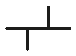
\includegraphics[scale=.5]{horizontalPattern}}}} 
% vertical pattern
\newcommand{\verticalPattern}{\smash{\raisebox{-.25cm}{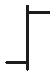
\includegraphics[scale=.5]{verticalPattern}}}} 

% Loday and anti-Loday accents (?)
\makeatletter
\newcommand{\oset}[3][0ex]{%
  \mathrel{\mathop{#3}\limits^{
    \vbox to#1{\kern-2\ex@
    \hbox{$\scriptstyle#2$}\vss}}}}
%
\newcommand{\uset}[3][0ex]{%
  \mathrel{\mathop{#3}\limits_{
    \vbox to#1{\kern-7\ex@
    \hbox{$\scriptstyle#2$}\vss}}}}
\makeatother
%
\newcommand{\loday}[1]{\smash{\overset{\frown}{#1}}}
\newcommand{\antiloday}[1]{\smash{\overset{\smile}{#1}}}
\newcommand{\upArc}[1]{\smash{\raisebox{.05cm}{$\uset[0ex]{#1}{\frown}$}}}
\newcommand{\downArc}[1]{\smash{\raisebox{-.05cm}{$\oset[.2ex]{#1}{\smile}$}}}
% yin and yang accents (?)
\newcommand{\yin}[1]{\smash{\overset{\sim}{#1}}}
\newcommand{\yang}[1]{\smash{\overset{\backsim}{#1}}}
\newcommand{\yinArc}[2]{\smash{\raisebox{.05cm}{$\uset[0ex]{#1}{\frown}$}\hspace{-.3ex}\raisebox{-.03cm}{$\oset[.2ex]{#2}{\smile}$}}}
\newcommand{\yangArc}[2]{\smash{\raisebox{-.03cm}{$\oset[.2ex]{#1}{\smile}$}\hspace{-.3ex}\raisebox{.05cm}{$\uset[0ex]{#2}{\frown}$}}}
% weak and strong equivalence on S_n
\newcommand{\weakeq}{\asymp}
\newcommand{\strongeq}{\mathbin{\smash{\begin{smallmatrix} \backsim \\[-.3cm] \sim \end{smallmatrix}}}}% % J: I would like to stack \backsim and \sim instead

% formating the table of contents
\setcounter{tocdepth}{4}
\makeatletter
\def\l@part{\@tocline{1}{8pt}{0pc}{}{}}
\def\l@section{\@tocline{1}{4pt}{0pc}{}{}}
\makeatother
\let\oldtocpart=\tocpart
\renewcommand{\tocpart}[2]{\sc\large\oldtocpart{#1}{#2}}
\let\oldtocsection=\tocsection
\renewcommand{\tocsection}[2]{\bf\oldtocsection{#1}{#2}}
\let\oldtocsubsubsection=\tocsubsubsection
\renewcommand{\tocsubsubsection}[2]{\quad\oldtocsubsubsection{#1}{#2}}

%%%%%%%%%%%%%%%%%%%%%%%%%%%%%%%%%%%%%%
%%%%%%%%%%%%%%%%%%%%%%%%%%%%%%%%%%%%%%

%\title{Rectangulation polytopes}
\title{Rectangulotopes}

\thanks{VP was partially supported by the Spanish grant PID2022-137283NB-C21 of MCIN/AEI/10.13039/501100011033 / FEDER, UE, by Departament de Recerca i Universitats de la Generalitat de Catalunya (2021 SGR 00697), by the French grant CHARMS (ANR-19-CE40-0017), and by the French--Austrian projects PAGCAP (ANR-21-CE48-0020 \& FWF I 5788).}

\author{Jean Cardinal}
\address{Université libre de Bruxelles (ULB)}
\email{jean.cardinal@ulb.be}
\urladdr{\url{https://jean.cardinal.web.ulb.be}}

\author{Vincent Pilaud}
\address{Universitat de Barcelona}
\email{vincent.pilaud@ub.edu}
\urladdr{\url{https://www.ub.edu/comb/vincentpilaud/}}

%%%%%%%%%%%%%%%%%%%%%%%%%%%%%%%%%%%%%%
%%%%%%%%%%%%%%%%%%%%%%%%%%%%%%%%%%%%%%

\begin{document}

\begin{abstract}
  Rectangulations are decompositions of a square into finitely many axis-aligned rectangles.
  We describe realizations of $(n-1)$-dimensional polytopes associated with two families of rectangulations composed of $n$ rectangles.
  They are defined as quotientopes of natural congruence relations on the weak Bruhat order on permutations in $\f{S}_n$, and their skeleta are flip graphs on rectangulations.
  We give simple vertex and facet descriptions of these polytopes, in particular elementary formulas for computing the coordinates of the vertex corresponding to each rectangulation, in the spirit of J.-L.~Loday's realization of the associahedron.
\end{abstract}

\maketitle

\tableofcontents

%%%%%%%%%%%%%%%%%%%%%%%%%%%%%%%%%%%%%%
%%%%%%%%%%%%%%%%%%%%%%%%%%%%%%%%%%%%%%

\section{Introduction}
\label{sec:intro}

%%%%%%%%%%%%%

\subsection{Polytopes of permutations, triangulations, and rectangulations}
\label{subsec:permTrianRect}

The encoding of combinatorial objects in the form of a polyhedral structure is a recurrent theme in geometric and algebraic combinatorics.
An elementary yet striking example of this idea is the \defn{permutahedron} $\Perm (n)$, defined as the convex hull of the points $\sum_{i\in [n]} \sigma^{-1}(i)\cdot \b{e}_i$, for all permutations $\sigma \in \f{S}_n$.
It is an $(n-1)$-dimensional polytope, whose facets are indexed by the proper nonempty subsets of $[n]$, and whose skeleton is the Cayley graph of the symmetric group for the generators consisting of adjacent transpositions.
See \cref{fig:quotientopes}\,(left) for an illustration when~$n = 4$.
The many generalizations and extensions of the permutahedra gave rise to a flourishing theory of \defn{deformed permutahedra}~\cite{MR2520477,Postnikov,MR4064768,MR4651496} (also call \defn{generalized permutahedra}, or \defn{polymatroids}).

Among those, the \defn{associahedron} is a classical, ubiquitous polytope, first defined by D.~Tamari~\cite{T51} and by J.~Stasheff~\cite{S63} in a topological context.
It has since then been identified as a fundamental object in many other areas of mathematics, including operads, cluster algebras, combinatorial Hopf algebras, and physics (see for instance the recent survey from V. Pilaud, F. Santos and G. Ziegler~\cite{PilaudSantosZiegler} and references therein).
It was first thought of as a purely combinatorial object, before various families of geometric realizations were shown to exist~\cite{MR1022776,MR1941227,MR2108555,MR3437894,MR2321739}.
The face lattice of the $(n-1)$-dimensional associahedron is the reverse inclusion poset of nonintersecting diagonals of a convex $(n+3)$-gon.
In particular, its skeleton is the \defn{flip graph} on \defn{triangulations} of the $(n+3)$-gon, or equivalently -- via a standard Catalan bijection -- the \defn{rotation graph} on \defn{binary trees} with $n$ internal nodes, the structure of which has been the subject of many investigations, with applications in computer science~\cite{MR928904,MR3197650}.
In 2004, J.-L.~Loday published the following elegant description of the associahedron~\cite{MR2108555}, giving a recipe for computing the coordinates of a vertex given the corresponding binary tree.
We note that the inequality description of the same polytope was actually provided in 1993 by S.~Shnider and S.~Sternberg~\cite{ShniderSternberg}, but Loday's vertex description largely popularized this realization.
See \cref{fig:quotientopes}\,(right) for an illustration when~$n = 4$.

\begin{theorem}
  \label{thm:loday}
  The associahedron is realized by the polytope~$\Asso (n) \subset \R^n$ defined equivalently as
  \begin{enumerate}[(i)]
  \item the convex hull of the points~$\sum_{i\in [n]} \ell^T_i\cdot r^T_i \cdot \b{e}_i$ for all binary trees~$T$ with $n$ internal nodes, where $\ell^T_i$ and $r^T_i$ denote the number of leaves in the left and right subtrees of $i$ in $T$, see~\cite{MR2108555},
  \item the intersection of the hyperplane defined by~$\sum_{i \in [n]} x_i = \binom{n+1}{2}$ with the halfspaces defined by~$\sum_{i \in I} x_i \le \#\set{J \text{ interval of } [n]}{I \cap J \ne \varnothing}$ for all intervals~$\varnothing \ne I \subsetneq [n]$, see~\cite{ShniderSternberg}.
  \end{enumerate}
\end{theorem}

A natural object associated with the associahedron is the \defn{Tamari lattice}, the cover graph of which is isomorphic to the skeleton of the associahedron~\cite{MR0146227,MR3235205}.
The Tamari lattice is known to be the quotient of the weak Bruhat order by a \defn{lattice congruence} relation called the \defn{sylvester congruence}~\cite{MR1654173,MR2142078}.
Answering a question of N.~Reading~\cite{MR2142177}, V.~Pilaud and F.~Santos~\cite{MR3964495} proved that with \emph{every} lattice congruence of the weak Bruhat order, one can associate a polytope whose skeleton is the cover graph of the lattice quotient, and more precisely whose normal fan is the \defn{quotient fan} defined by gluing the cones of the \defn{braid fan} (the type $A$ Coxeter arrangement) that belong to the same congruence class.
Those polytopes are deformed permutahedra that they called \defn{quotientopes}.
Associahedra are therefore the quotientopes of the sylvester congruence of the weak Bruhat order whose classes are in bijection with triangulations.

The goal of this paper is to describe the geometry of the quotientopes for two particular congruences of the weak Bruhat order whose classes are in bijection with equivalence classes of rectangulations, defined as decompositions of a square into rectangles.

\subsection{Weak and strong rectangulations}

The combinatorics of rectangulations has been studied for nearly two decades~\cite{MR2233287,MR2763051,MR2871762,MR2864445,MR3084577,MR3192492,MR3878132,MR4598046}.
Interestingly, several combinatorial results were initially motivated by applications to the design of \defn{floorplans} for very large scale integrated circuits, and published in electrical engineering journals, see for instance R. Fujimaki, Y. Inoue, and T. Takahashi~\cite{FT07,TF08,ITF09,FIT09}.

We define a \defn{rectangulation} of size $n$ as a decomposition of the square into $n$ axis-parallel rectangles with disjoint interiors.
The \defn{segments} of a rectangulation are the inclusionwise maximal line segments composed of edges of the rectangles, excluding the edges of the decomposed square.
We suppose throughout that no four rectangles have a common vertex, hence that the rectangulations are \defn{generic} in that sense.

In order to focus on the combinatorial structure of a rectangulation, we introduce two equivalence relations between rectangulations.
We say that a rectangle $r$ is \defn{above} another rectangle $s$ (and $s$ is \defn{below} $r$) if either the bottom edge of $r$ lies in the same segment as the top edge of $s$, or if $r$ is above another rectangle $t$ that is above $s$.
Similarly, a rectangle $r$ is \defn{on the left of} another rectangle $s$ (and $s$ is \defn{on the right of} $r$) if either the right edge of $r$ lies in the same segment as the left edge of $s$, or if $r$ is on the left of another rectangle $t$ that is on the left of $s$.
Two rectangulations are said to be \defn{weakly equivalent} if there exists a bijection between their rectangles that preserves the above-below and left-right relations between the rectangles.
Weak equivalence classes of rectangulations will be referred to as \defn{weak rectangulations}.
(Note that this is a slight, yet convenient abuse of terminology, as weak rectangulations are really sets of rectangulations.)
On the other hand, two rectangulations are said to be \defn{strongly equivalent} when there exists a bijection between their rectangles that not only preserves the above-below and left-right relations, but also the adjacency relation between rectangles.
We will naturally refer to strong equivalence classes of rectangulations as \defn{strong rectangulations}.

In order to make sense of these definitions, it is useful to consider \defn{wall slides} in a rectangulation: the local changes consisting of shifting a horizontal segment vertically, or a vertical segment horizontally, while extending or shortening the incident segments accordingly.
Performing a wall slide in a rectangulation $R$ leads to a rectangulation that is always weakly equivalent to $R$.
However, if the wall slide changes the adjacency relation between the rectangles, then the resulting rectangulation is not strongly equivalent to $R$ anymore.
This is illustrated in Figure~\ref{fig:rectequiv}.
A \defn{diagonal rectangulation} is a rectangulation in which every rectangle intersects the top-left to bottom-right diagonal of the square, see Figure~\ref{fig:weakRectangulation}.
It is simple to check that every weak rectangulation has a diagonal representative, hence weak rectangulations can also be thought of as diagonal rectangulations.

\begin{figure}
	\caption{Weak and strong equivalence between rectangulations.}
	\label{fig:rectequiv}
\end{figure}

\subsection{Weak and strong rectangulotopes}

Weak and strong rectangulations of size $n$ have been shown to define congruences of the weak Bruhat order on $\f{S}_n$.

The \defn{weak rectangulation congruence} (or \defn{Baxter congruence}) was first explicitly studied by S.~Law and N.~Reading~\cite{MR2871762} and revisited in~\cite[Thm.~1.1 \& Exm.~4.10]{Reading-arcDiagrams}.
Its classes are in bijection with with weak rectangulations, but also with \defn{Baxter permutations}~\cite{MR0491652,MR0555815}, \defn{twin binary trees}~\cite{MR1417289,MR2914637}, and many other combinatorial families~\cite{MR2763051}. 
The corresponding quotientopes will be referred to as the \defn{weak rectangulotopes} and denoted by $\WRP(n)$.

The \defn{strong rectangulation congruence} was introduced by N.~Reading~\cite{MR2864445}, revisited in~\cite[Thm.~1.2 \& Exm.~4.11]{Reading-arcDiagrams}, and studied more recently by E.~Meehan~\cite{MR3697823}, and A.~Asinowski, J.~Cardinal, S.~Felsner, and É.~Fusy~\cite{ACFF24}.
Its classes are in bijection with strong rectangulations.
The corresponding quotientopes will be referred to as the \defn{strong rectangulotopes} and denoted by~$\SRP(n)$.

An important motivation for studying these quotientopes is the informative structure of their skeleta, which are \defn{flip graphs} on the rectangulations.
A flip is a local, reversible change in the structure of the rectangulation.
Flips in rectangulations come in three flavors:
\begin{description}
\item[Simple flips] replace a vertical segment incident to exactly two rectangles by a horizontal segment, and vice-versa.
\item[Pivoting] operations transform a pair of adjacent rectangles whose union is not a rectangle, changing a left-right pair into an above-below pair, and vice-versa.
\item[Wall slide] flips are wall slides that modify the adjacency of the rectangles, removing exactly one adjacency and adding exactly one. These flips are only relevant in strong rectangulations.
\end{description}

The various types of flips are illustrated in Figure~\ref{fig:flips}.
We refer to S.~Law and N.~Reading~\cite{MR2871762}, J.~Cardinal, V.~Sacrist\'an, and R.~Silveira~\cite{MR3878132}, E.~Meehan~\cite{MR3697823}, and A.~Asinowski, J.~Cardinal, S.~Felsner, and \'E.~Fusy~\cite{ACFF24} for detailed descriptions of the flip graphs on both weak and strong rectangulations.
Just like associahedra encode the rotation graphs on binary trees, the rectangulotopes directly yield flip graphs on rectangulations.

\begin{figure}
	\caption{Three types of flips between rectangulations.}
	\label{fig:flip}
\end{figure}

\begin{lemma}
  The skeleton of $\WRP(n)$ (resp.~of $\SRP(n)$) is isomorphic to the flip graph on weak (resp.~strong) rectangulations of size~$n$.
  \vincent{I would leave that in the text, not in a proper thm environment...}
\end{lemma}

Rectangulotopes enrich the family of natural quotientopes, alongside associahedra, permutreehedra~\cite{MR3856522}, certain brick polytopes~\cite{PilaudSantos-brickPolytopes, PilaudStump-brickPolytopes, Pilaud-brickAlgebra}, and certain graphical zonotopes~\cite{Pilaud-brickAlgebra, Pilaud-acyclicReorientationLattices}, providing instructive examples of application of the theory of lattice congruences to concrete combinatorial objects.
Our main results are elementary vertex and facet descriptions of both families of quotientopes.
For vertices, we describe the coordinates of the vertex corresponding to a weak or strong rectangulation with simple product formulas in the spirit of J.-L.~Loday's realization in~\cref{thm:loday}.
As mentioned in~\cite{PilaudSantosZiegler}, there is no such formula for arbitrary quotientopes, which makes rectangulotopes join the restricted club of Loday type quotientopes, jointly with associahedra and permutreehedra~\cite{MR3856522}.
For facets, we show that both weak and strong rectangulotopes have $2^n-2$ facets (the maximal possible number of facets of a deformed permutahedron), and provide simple formulas for the right hand side of the inequality corresponding to a given proper nonempty subset of~$[n]$.

We now give the necessary definitions for precisely stating these vertex and facet descriptions of the weak and strong rectangulotopes.

\subsection{Source and target trees of a rectangulation}
\label{subsec:sourceTargetTrees}

% jean:{Here only give the definitions allowing to state the results.}

\begin{figure}
	\centerline{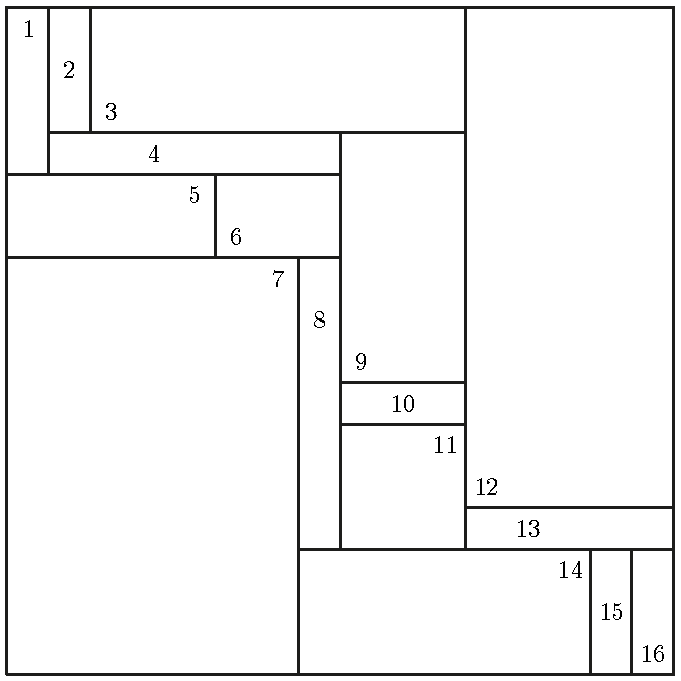
\includegraphics[width=.5\textwidth]{weakRectangulation} \qquad 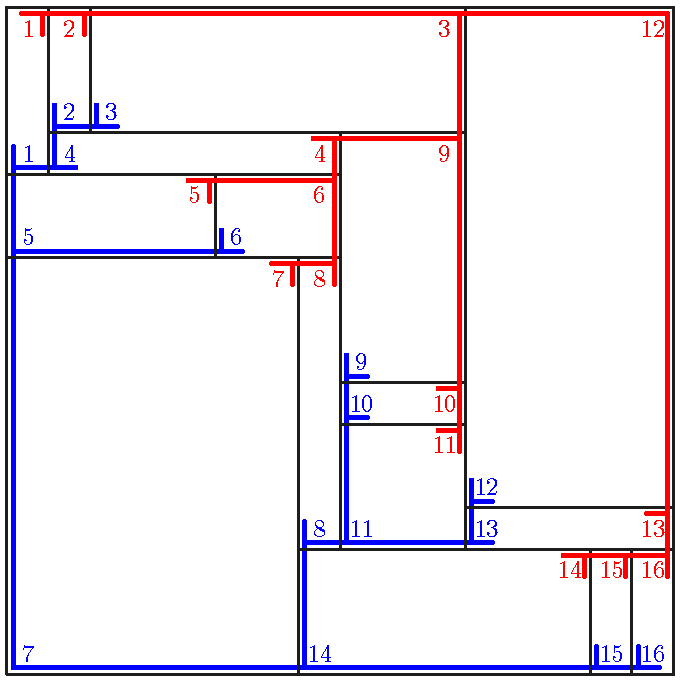
\includegraphics[width=.5\textwidth]{weakRectangulationTrees}}
	\caption{A diagonal rectangulation (left) and its pair of twin binary trees (right). Example from \cite{ACFF24}.}
	% The corresponding twisted Baxter permutation is $[7, 5, 1, 14, 8, 6, 4, 2, 11, 10, 9, 3, 15, 16, 13, 12]$ and its inverse is $[3, 8, 12, 7, 2, 6, 1, 5, 11, 10, 9, 16, 15, 4, 13, 14]$.
	\label{fig:weakRectangulation}
\end{figure}

\begin{figure}
	\centerline{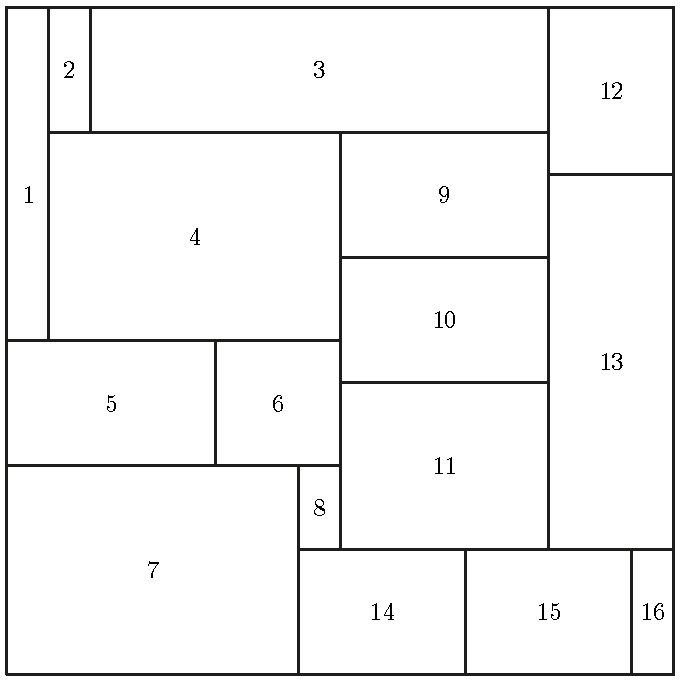
\includegraphics[width=.5\textwidth]{strongRectangulation} \qquad 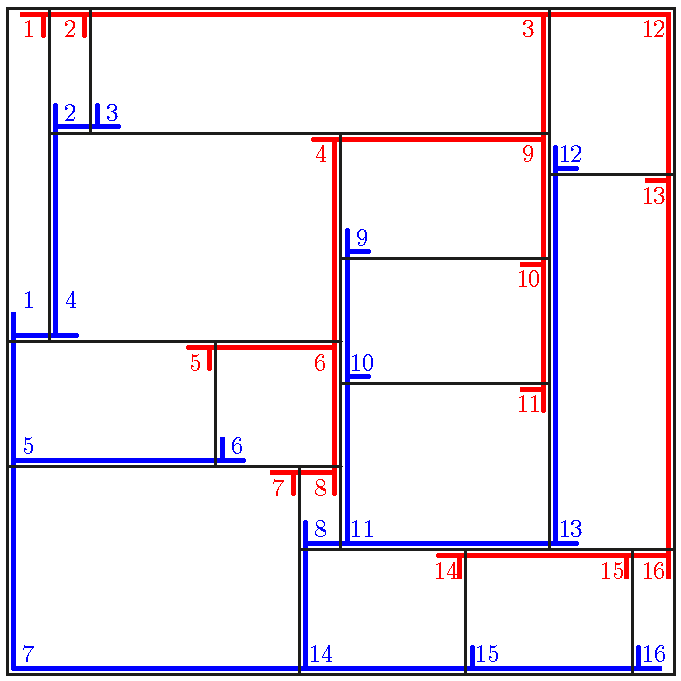
\includegraphics[width=.5\textwidth]{strongRectangulationTrees}}
	\caption{A (non-diagonal) rectangulation (left) and its pair of intertwining binary trees (right). Example from \cite{ACFF24}.}
        % The corresponding $2$-clumped permutation is $[7,5,14,8,1,6,15,11,4,10,16,2,9,13,3,12]$ and its inverse is $[5, 12, 15, 9, 2, 6, 1, 4, 13, 10, 8, 16, 14, 3, 7, 11]$.
        \label{fig:strongRectangulation}
\end{figure}

Fix a rectangulation~$R$ of size~$n$, and consider the directed graph~$D(R)$ whose vertex set is the set of all vertices of~$R$, and whose edges are obtained as follows.
For each rectangle~$r$ of~$R$, we include in~$D(R)$ four edges joining the vertices of~$r$, where the horizontal edges are oriented from left to right, and the vertical edges are oriented from bottom to top.
Hence, the bottom left corner of~$r$ is its source~$s(r)$, while its top right corner is its target~$t(r)$.
Note that since~$R$ is generic, the sources~$\set{s(r)}{r \in [n]}$ and the targets~$\set{t(r)}{r \in [n]}$ are disjoint.
The \defn{source tree}~$S(R)$ (resp.~\defn{target tree}~$T(R)$) is the subgraph of~$D(R)$ induced by the sources~$\set{s(r)}{r \in [n]}$ (resp.~by the targets~$\set{t(r)}{r \in [n]}$).
See \cref{fig:strongRectangulation}.

\begin{lemma}
The source tree~$S(R)$ (resp.~target tree~$T(R)$) is a binary tree, rooted at the bottom left (resp.~top right) corner of~$R$, and oriented from (resp.~towards) its root.
\end{lemma}

\begin{comment}
\begin{proof}
By symmetry, we only prove the statement for the source tree~$S(R)$.
As the rectangulation is generic, each source~$s(r)$ distinct from the bottom left corner of~$R$ is either on the top edge of a rectangle~$r'$ or on the right edge of a rectangle~$r'$ (but not both).
This shows that~$r$ distinct from the bottom left rectangle of~$R$ has a unique parent~$r'$ in~$S(R)$, so that~$S(R)$ is indeed a tree on~$[n]$.
This tree is binary as each node has at most one vertical child and one horizontal child, and no other children.
\end{proof}
\end{comment}

We complete each node of~$S(R)$ and~$T(R)$ with a vertical (resp.~horizontal) leaf if it has no vertical (resp.~horizontal) child, see \cref{fig:strongRectangulation}.
If the rectangulation $R$ is diagonal, we retrieve the well-studied pair of twin binary trees~\cite{MR1417289,MR2914637}.
Recall that the \defn{inorder labeling} of a binary tree~$T$ is the labeling of the nodes of~$T$ such that the label of each node~$t$ of~$T$ is larger than all labels in the left subtree of~$t$ and larger than all labels in the right subtree of~$t$.

\begin{lemma}
For any rectangle~$r$ of~$R$, the inorder label of the source~$s(r)$ in~$S(R)$ coincides with the inorder label of the target~$t(r)$ in~$T(R)$.
\end{lemma}

This enables to unambiguously label the rectangles of~$R$ by the inorder.
The resulting labeling coincides with the NW--SE labeling of~\cite{ACFF24}.
From now on, the labels of the rectangles in a rectangulations are the inorder labels, and the two trees $T(R)$ and $S(R)$ are defined on the vertex set $[n]$ accordingly.
For each $i\in [n]$, we refer to its two subtrees in $T(R)$ as the \defn{horizontal} and \defn{vertical subtrees}, and similarly for $S(R)$.

%%%%%%%%%%%%%

\subsection{Weak rectangulotopes}
\label{subsec:weakRectangulotopes}

Our first results are simple vertex and facet descriptions of the weak rectangulotopes~$\WRP(n)$.
For the vertices, we provide a concise formula for the coordinates, that consists of applying J.-L.~Loday's formula on each of the source and target trees of the rectangulation.
For the facets, we combine the right hand sides of two opposite associahedra to obtain those of the weak rectangulotopes.
This materializes the result of Law and Reading that the weak rectangulotopes are Minkowski sums of two opposite associahedra~\cite{MR2871762}.

\Jean{We need to make it clear whether $\WRP (n)$ is the proposed realization or just the combinatorial type. I was thinking the latter. Then we can change the sentence ``The weak rectangulotope is realized by the polytope~$\WRP (n)$...'' by ``The weak rectangulotope $\WRP (n)$ is realized by:~''. Otherwise, refrain from using $\WRP (n)$ before here.}

\begin{theorem}
  The weak rectangulotope is realized by the polytope~$\WRP (n) \subset \R^n\!$ defined equivalently~as
  \begin{enumerate}[(i)]
  \item the convex hull of the points
  $\sum_{i\in [n]} (\loday{w}^R_i - \antiloday{w}^R_i)\cdot \b{e}_i$ for all weak rectangulations $R$ of size~$n$,
  with
  \[
%  \begin{split}
%    \loday{w}^R_i \eqdef & h(T, i)\cdot v(T,i) \\
%    \antiloday{w}^R_i \eqdef & h(S, i)\cdot v(S,i),
%  \end{split}
    \loday{w}^R_i \eqdef h^T_i\cdot v^T_i
    \qquad\text{and}\qquad
    \antiloday{w}^R_i \eqdef h^S_i\cdot v^S_i,
  \]
  where~$S$ and~$T$ are the source and target trees of the rectangulation~$R$, and $h^T_i$ and $v^T_i$ denote the number of leaves in the horizontal and vertical subtrees of $i$ in~$T$,
  \item the intersection of the hyperplane defined by~$\sum_{i \in [n]} x_i = \binom{n+1}{2}$ with the halfspaces defined by~$\sum_{i \in S} x_i \le \#\set{I \text{ interval of } [n]}{I \not\subseteq S \text{ and } I \not\subseteq [n] \ssm S}$ for all subsets~$\varnothing \ne S \subsetneq [n]$.
  \end{enumerate}
\end{theorem}

\begin{example}
  The vertex of~$\WRP (16)$ corresponding to the weak rectangulation of \cref{fig:weakRectangulation} is
  \[
  (-3, 0, 26, 2, -9, 5, -69, -4, 17, 0, -8, 59, 2, -20, 0, 2).
  \]
  For instance, the $4$th coordinate is $h^T_4 \cdot v^T_4 - h^S_4 \cdot v^S_4 = 1 \cdot 5 - 1 \cdot 3 = 2$.
  \vincent{give also a relevant example of facet...}
\end{example}

%%%%%%%%%%%%%

\subsection{Strong rectangulotopes}
\label{subsec:strongRectangulotopes}

In order to exhibit a similar realization for the strong rectangulotopes, we need to count subsets of leaves that lie in some subtrees of both the source and target trees of a rectangulation.
Two leaves of the trees $T(R)$ and $S(R)$ are said to be \defn{common leaves} if the edges to their parents lie on the same segment of $R$.
We denote by $i \, \backslash \, j$ the situation where the rectangle labeled $i$ touches the rectangle labeled $j$ either from the left or from below in $R$.
We also use the Iverson bracket $\llbracket \varphi\rrbracket$, which is equal to 1 if $\varphi$ holds, and 0 otherwise.

\begin{theorem}
  The $(n-1)$-dimensional strong rectangulotope is realized by the polytope~$\SRP (n)$ defined equivalently as
  \begin{enumerate}[(i)]
  \item convex hull of the points
  \[
  \sum_{i,j\in [n], i< j} (\yin{w}^R_{i,j} - \yang{w}^R_{i,j})\cdot (\b{e}_i - \b{e}_j),
  \]
   for all strong rectangulations $R$ of size~$n$, with
  \[
%  \begin{split}
%    \yin{w}_{i,j} \eqdef & h(T, i) \cdot cv (T, S, i, j)\cdot h(S, j)\cdot \llbracket \neg i\backslash j \rrbracket \\% \text { if not } i\backslash j, \text{and } 0\text{ otherwise.} \\ % \neg i|j \text{ and } \neg \frac{\ j\ }i ] \\
%    \yang{w}_{i,j} \eqdef & v(S, i) \cdot ch (S, T, i, j)\cdot v(T, j) \cdot \llbracket \neg j\backslash i \rrbracket,
%  \end{split}
    \yin{w}^R_{i,j} \eqdef h^T_i \cdot cv^{T,S}_{i,j}\cdot h^S_ j\cdot \llbracket \neg \, i \, \backslash \, j \rrbracket
    \qquad\text{and}\qquad
    \yang{w}^R_{i,j} \eqdef v^S_i \cdot ch^{S,T}_{i,j}\cdot v^T_j \cdot \llbracket \neg \, j \, \backslash \, i \rrbracket,
  \]
 where:
  \begin{itemize}
  \item $S$ and $T$ are the source and target trees of the rectangulation~$R$,
  \item $h^T_i$ and $v^T_i$ denote the number of leaves in the horizontal and vertical subtrees of $i$ in~$T$,
  \item $ch^{T,S}_{i,j}$ (resp.~$cv^{T,S}_{i,j}$) denote the number of common leaves of the horizontal (resp.~vertical) subtree of $i$ in $T$ and the horizontal (resp.~vertical) subtree of $j$ in $S$.
  \end{itemize}
  \item the intersection of the hyperplane defined by~$\sum_{i \in [n]} x_i = \binom{n+1}{2}$ with the halfspaces defined by~$\sum_{i \in S} x_i \le \#\set{I,J}{I \not\subseteq S \text{ and } J \not\subseteq [n] \ssm S} + \#\set{I,J}{I \not\subseteq [n] \ssm S \text{ and } J \not\subseteq S}$ for all subsets~$\varnothing \ne S \subsetneq [n]$, where~$I,J$ in the sets denote nonempty and consecutive intervals of~$[n]$.
  \end{enumerate}
\end{theorem}

% jean:{Is there better way to write this down/compute? Here we do not take advantage of the fact that at most one of the two factors $\yin{w}_{i,j}$ and $\yang{w}_{i,j}$ is nonzero.}

\begin{example}
  The vertex of~$\SRP (16)$ corresponding to the strong rectangulation of \cref{fig:strongRectangulation} is
  \[
  ???
  \]
  For instance, the $4$th coordinate is $???$.
  \vincent{give also a relevant example of facet...}
\end{example}

%%%%%%%%%%%%%

\subsection{Plan of the paper}
\label{subsec:plan}

\cref{sec:quotientopes} is dedicated to the background on quotientopes and their realizations as Minkowski sums of \defn{shard polytopes}, due to A.~Padrol, V.~Pilaud, and J.~Ritter~\cite{MR4584712}, which will be our main tool throughout. \cref{sec:weakRectangulotopes} details the case of weak rectangulations, while \cref{sec:strongRectangulotopes} deals with strong rectangulations. In both cases, in addition to the vertex coordinates, we also give the submodular functions defining the polytopes.

%%%%%%%%%%%%%%%%%%%%%%%%%%%%%%%%%%%%%%

\subsection*{Acknowledgments}

This work was initiated at the Workshop on Combinatorics, Algorithms, and Geometry held on March 4-8, 2024 in Dresden, Germany.
The authors thank Namrata and Torsten M\"utze for the organization and the other participants of the workshop for the stimulating interactions, notably on other combinatorial aspects of rectangulations.

%%%%%%%%%%%%%%%%%%%%%%%%%%%%%%%%%%%%%%
%%%%%%%%%%%%%%%%%%%%%%%%%%%%%%%%%%%%%%

\section{Quotientopes}
\label{sec:quotientopes}

We now briefly recall some results on the weak Bruhat order and its quotients, both from a lattice and geometric perspectives.
We refer to \cite{Reading-arcDiagrams, MR3645055, MR3645056, MR4584712} for details.
% J: Reading-Chapters: which one is this ?

\begin{figure}
	\capstart
	\centerline{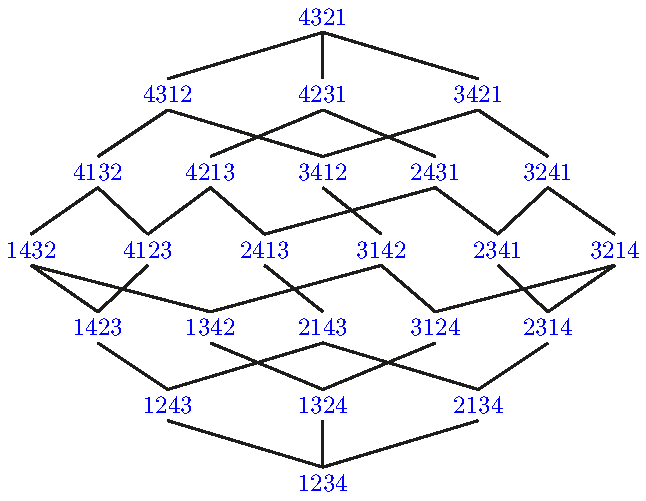
\includegraphics[scale=.6]{weakOrderLeft4} \; 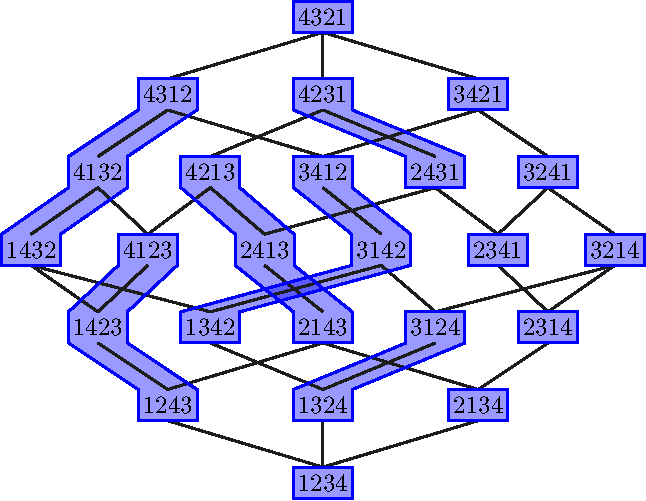
\includegraphics[scale=.6]{weakOrderCongruence4} \; 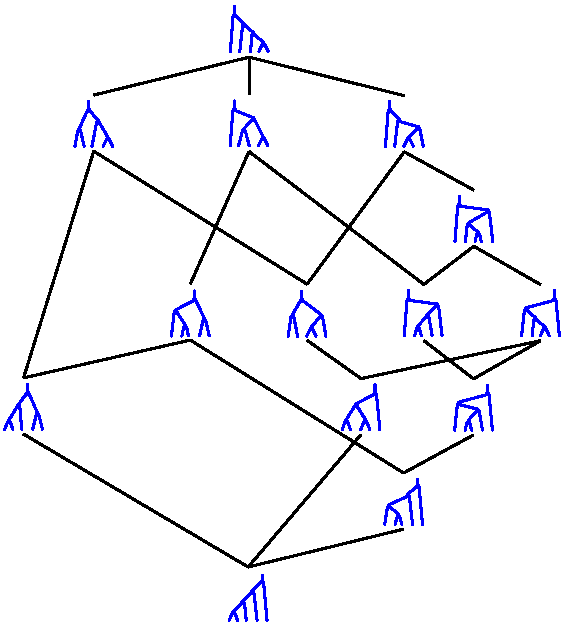
\includegraphics[scale=.48]{TamariLattice4}}
	\caption{The weak Bruhat order on~$\f{S}_4$ (left), the sylvester congruence~$\equiv_\textrm{sylv}$~(middle), and the Tamari lattice (right). \cite[Fig.~1 \& 2]{MR3964495}}
	\label{fig:sylvesterCongruence}
\end{figure}

%%%%%%%%%%%%%

\subsection{Weak order and noncrossing arc diagrams}
\label{subsec:noncrossingArcDiagrams}

Denote by~$\f{S}_n$ the set of permutations of~$[n]$.
The \defn{inversion set} of~$\sigma \in \f{S}_n$ is~$\inv(\sigma) \eqdef \set{(\sigma_i, \sigma_j)}{1 \le i < j \le n \text{ and } \sigma_i > \sigma_j}$.
The \defn{weak Bruhat order}\footnote{The weak Bruhat order is usually just referred to as the weak order. In this paper, we prefer to use weak Bruhat order to avoid any confusion with the weak poset defined on weak rectangulations.} is the lattice on the permutations of~$\f{S}_n$ defined by the inclusion of their inversion sets.
See \cref{fig:sylvesterCongruence}\,(left).
Note that the cover relations in the weak Bruhat order are given by the transpositions of two adjacent letters.
%The weak Bruhat order is known to be a congruence uniform lattice~\cite{}.
%In particular, it is join semidistributive, so that any permutation admits a canonical join representation.

An \defn{arc} on~$[n]$ is a quadruple~$(a, b, A, B)$ where~$1 \le a < b \le n$ and~$A \sqcup B$ forms a partition of the interval~${]a,b[} \eqdef \{a+1, \dots, b-1\}$.
We represent an arc by an abscissa monotone curve wiggling around the horizontal axis, starting at point~$a$ and ending at point~$b$, and passing above the points of~$A$ and below the points of~$B$.
A \defn{noncrossing arc diagram} on~$[n]$ is a collection of arcs on~$[n]$ where any two arcs do not cross in their interior and have distinct left endpoints and distinct right endpoints (but the right endpoint of an arc can be the left endpoint of another arc).

\vspace{-.1cm}
\parpic(4cm,2.5cm)(10pt, 150pt)[r][b]{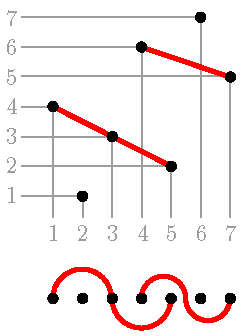
\includegraphics[scale=.9]{arcDiagram}}{
In~\cite{Reading-arcDiagrams}, N.~Reading defined an elegant bijection between permutations of~$[n]$ and noncrossing arc diagrams on~$[n]$.
It sends a permutation~$\sigma$ to the noncrossing arc diagram with an arc~$(\sigma_{j+1}, \sigma_j, A_j, B_j)$ for each descent~$j \in [n-1]$ of~$\sigma$ (\ie with~$\sigma_j > \sigma_{j+1}$), where

\vspace{-.2cm}
\begin{minipage}{10cm}
\begin{align*}
A_j & \eqdef \set{\sigma_i}{1 \le i < j \text{ and } \sigma_{j+1} < \sigma_i < \sigma_j} \\
\text{and} \qquad
B_j & \eqdef \set{\sigma_k}{j+1 < k \le n \text{ and } \sigma_{j+1} < \sigma_k < \sigma_j}.
\end{align*}
\end{minipage}

\vspace{.2cm}
\noindent
As illustrated on the right, this can also been visualized by representing the table~$(\sigma_j,j)$ of the permutation~$\sigma$, drawing the segments corresponding to the descents of~$\sigma$, and letting all points fall on the horizontal axis, allowing the segments to bend but not to cross each other nor to pass through a point.
The single arcs correspond to permutations with a single descent, that is, to join irreducible permutations of the weak Bruhat order.
In general, the noncrossing arc diagram of a permutation~$\sigma$ actually encodes the canonical join representation of~$\sigma$ in the weak Bruhat order (which was known to exist, as the weak Bruhat order is join semidistributive).
See~\cite{Reading-arcDiagrams} for details.
}

%%%%%%%%%%%%%

\subsection{Quotients and arc ideals}
\label{subsec:arcIdeals}

A \defn{lattice congruence} of the weak Bruhat order is an equivalence relation~$\equiv$ on~$\f{S}_n$ that respects the meet and join operations, \ie such that $x \equiv x'$ and~$y \equiv y'$ implies $x \meet y \, \equiv \, x' \meet y'$ and~$x \join y \, \equiv \, x' \join y'$.
The \defn{lattice quotient}~$\f{S}_n/{\equiv}$ is the lattice on the congruence classes of~$\equiv$ where~$X \le Y$ if and only if there exist~$x \in X$ and~$y \in Y$ such that~$x \le y$, and~$X \meet Y$ (resp.~$X \join Y$) is the congruence class of~$x \meet y$ (resp.~$x \join y$) for any~$x \in X$~and~$y \in Y$.

For instance, the sets of linear extensions of binary trees (labeled in inorder and oriented toward their roots) are the classes of the \defn{sylvester congruence}~\cite{HivertNovelliThibon-binarySearchTrees}.
See \cref{fig:sylvesterCongruence}\,(middle).
The quotient of the weak Bruhat order by the sylvester congruence is the classical \defn{Tamari lattice}.
See \cref{fig:sylvesterCongruence}\,(right).

Respecting the meet and join operation is a strong condition that imposes additional structure on~$\equiv$.
In fact, all the congruence classes of~$\equiv$ are intervals of the weak Bruhat order, and the quotient~$\f{S}_n/{\equiv}$ is isomorphic (as a poset) to the subposet of the weak Bruhat order induced by permutations which are minimal in their class.
Moreover, the latter are precisely the permutations whose noncrossing arc diagrams only use arcs corresponding to join irreducible permutations which are minimal in their class, and we denote by~$\c{A}_\equiv$ this set of arcs.
In other words, the classes of~$\equiv$ are in bijection with noncrossing arc diagrams using only arcs in~$\c{A}_\equiv$.
This bijection actually translates the fact that canonical join representations behave properly under lattice quotients.

%Moreover, the sets of arcs of the form~$\c{A}_\equiv$ are easily described.
\vspace{-.15cm}
\parpic(5cm,2.8cm)(10pt, 90pt)[r][b]{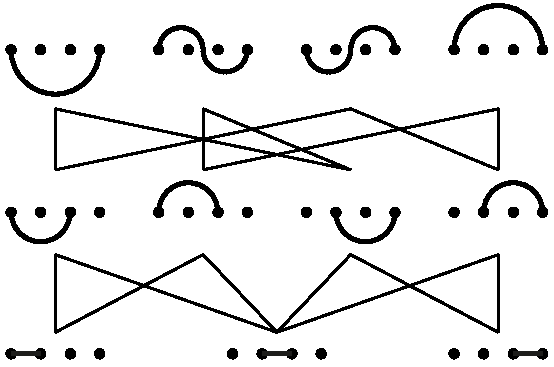
\includegraphics[scale=.5]{subarcOrder}}{
An arc~$(a, b, A, B)$ is a \defn{subarc} of an arc~$(a', b', A', B')$ if \linebreak $a' \le a < b \le b$ and~$A \subseteq A'$ while~$B \subseteq B'$.
An \defn{arc ideal} is a subset of arcs closed by subarcs.
The map~${\equiv} \mapsto \c{A}_\equiv$ is a bijection between the lattice congruences of the weak Bruhat order and the arc ideals.
In other words, the lattice of congruences of the weak Bruhat order is distributive, and its poset of join irreducibles is isomorphic to the subarc order, illustrated on the right for~$n = 4$.
}

%%%%%%%%%%%%%

\subsection{Quotient fans and shards}
\label{subsec:quotientFans}

\begin{figure}[b]
	\capstart
	\centerline{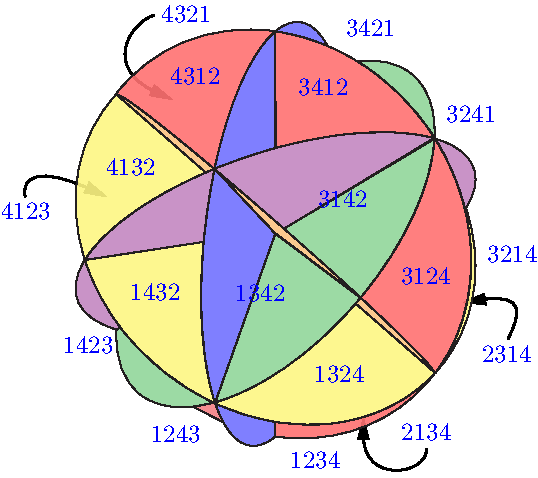
\includegraphics[scale=.6]{braidFanLeft4} \qquad \raisebox{-.3cm}{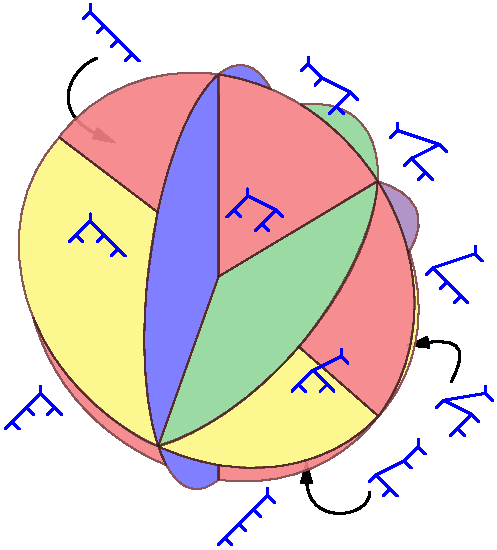
\includegraphics[scale=.6]{sylvesterFan4}}}
	\caption{The braid fan (left) and the sylvester fan (right). \cite[Fig.~1]{MR3964495} \&~\cite[Fig.~5]{MR4584712}}
	\label{fig:fans}
\end{figure}

The \defn{braid arrangement} is the hyperplane arrangement consisting of the hyperplanes~$\set{\b{x} \in \R^n}{x_a = x_b}$ for all~$1 \le a < b \le n$.
It has a chamber for each permutation~$\sigma$ of~$[n]$, given by the set of vectors whose coordinates are ordered as~$\sigma$.
See \cref{fig:fans}\,(left).

The \defn{shard} of an arc~$(a, b, A, B)$ is the piece of the braid hyperplane~${x_a = x_b}$ defined by the inequalities~$x_{a'} < x_a$ for all~$a' \in A$ and~$x_b < x_{b'}$ for all~$b' \in B$.
%$\Sigma(a, b, A, B) \eqdef \set{\b{x} \in \R^n}{x_a = x_b \text{ and } x_{a'} < x_a \text{ for all } a' \in A \text{ and }  x_b < x_{b'} \text{ for all } b' \in B}$.
In other words, the shards decompose each hyperplane~$x_a = x_b$ of the braid arrangement into~$2^{b-a-1}$ cones.

The \defn{quotient fan} of a congruence~$\equiv$ of the weak Bruhat order is the polyhedral fan~$\c{F}_\equiv$~where
\begin{itemize}
\item the maximal cones are obtained by glueing together the chambers of the braid arrangement corresponding to permutations in the same congruence class of~$\equiv$,
\item the union of the codimension~$1$ cones is the union of the shards of the arcs of~$\c{A}_\equiv$.
\end{itemize}
(These two descriptions are equivalent.)
By construction, the braid fan refines the quotient fan~$\c{F}_\equiv$, and the dual graph of the quotient fan~$\c{F}_\equiv$ is isomorphic to the cover graph of the quotient~$\f{S}_n/{\equiv}$.
For instance, \cref{fig:fans}\,(right) represents the \defn{sylvester fan} (the quotient fan of the sylvester congruence of \cref{fig:sylvesterCongruence}\,(middle)) for~$n = 4$, whose dual graph is the cover graph of the Tamari lattice of \cref{fig:sylvesterCongruence}\,(right).

%%%%%%%%%%%%%

\subsection{Quotientopes and shard polytopes}
\label{subsec:quotientopes}

\begin{figure}
	\capstart
	\centerline{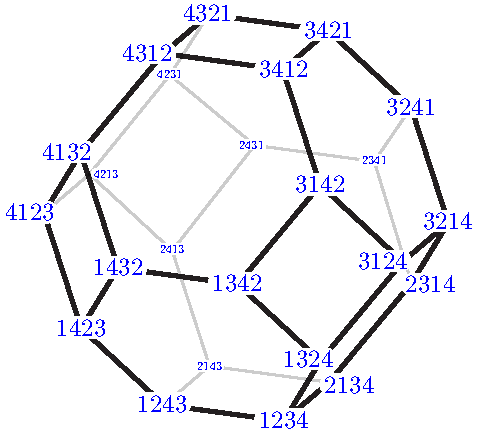
\includegraphics[scale=.6]{permutahedronLeft4} \qquad \raisebox{-.4cm}{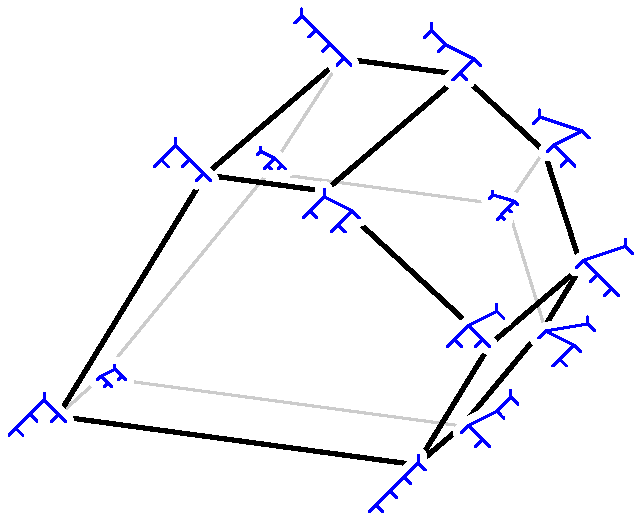
\includegraphics[scale=.6]{associahedron4}}}
	\caption{The permutahedron~$\Perm(4)$ (left) and the associahedron~$\Asso(4)$. \cite[Fig.~1]{MR3964495} \&~\cite[Fig.~5]{MR4584712}}
	\label{fig:quotientopes}
\end{figure}

A \defn{quotientope} for a lattice congruence~$\equiv$ of the weak Bruhat order is a polytope whose normal fan is the quotient fan~$\c{F}_\equiv$.
In particular, the skeleton of a quotientope is isomorphic to the cover graph of the quotient~$\f{S}_n/{\equiv}$.
For instance, the associahedron~$\Asso(n)$ (\cref{fig:quotientopes}\,(right) when~$n = 4$)  is a quotientope for the sylvester congruence (\cref{fig:sylvesterCongruence}\,(middle) when~$n = 4$), its normal fan is the sylvester fan (\cref{fig:fans}\,(right) when~$n = 4$), and its skeleton is the cover graph of the Tamari lattice (\cref{fig:sylvesterCongruence}\,(right) when~$n = 4$).
The existence of quotientopes was first proved in \cite{MR3964495} and later better understood in~\cite{MR4584712} using Minkowski sums of shard polytopes.

The \defn{Minkowski sum} of two polytopes~$\polytope{P}$ and~$\polytope{Q}$ is~$\polytope{P} + \polytope{Q} \eqdef \set{\b{p} + \b{q}}{\b{p} \in \polytope{P} \text{ and } \b{q} \in \polytope{Q}}$.
Recall that for any vector~$\b{v} \ne \b{0}$, the face of~$\polytope{P} + \polytope{Q}$ maximizing the scalar product with~$\b{v}$ is the Minkowski sum of the faces of~$\polytope{P}$ and~$\polytope{Q}$ maximizing the scalar product with~$\b{v}$.
In particular, if~$\b{v}$ is a generic direction, the vertex of~$\polytope{P} + \polytope{Q}$ extremal in direction~$\b{v}$ is just the sum of the vertices of~$\polytope{P}$ and~$\polytope{Q}$ that are extremal in direction~$\b{v}$.
Moreover, the normal fan of the Minkowski sum~$\polytope{P} + \polytope{Q}$ is the common refinement of the normal fans of~$\polytope{P}$ and~$\polytope{Q}$.

Consider an arc~$\alpha \eqdef (a, b, A, B)$ on~$[n]$.
An \defn{$\alpha$-alternating matching} is a sequence~$a \le i_1 < j_1 < i_2 < j_2 < \dots < i_q < j_q \le b$ such that~$i_p \in \{a\} \cup A$ and~$j_p \in \{b\} \cup B$ for all~$p \in [q]$.
Its \defn{characteristic vector} is~$\sum_{p \in [q]} \b{e}_{i_p} - \b{e}_{j_p}$.
The \defn{shard polytope} of~$\alpha$ is the convex hull~$\SP(\alpha)$ of the characteristic vectors of all $\alpha$-alternating matchings.
It was shown in~\cite{MR4584712} that any Minkowski sum of positive scalings of the shard polytopes~$\SP(\alpha)$ for all arcs~$\alpha$ in the arc ideal~$\c{A}_\equiv$ is a quotientope for~$\equiv$.

\begin{figure}
	\capstart
	\centerline{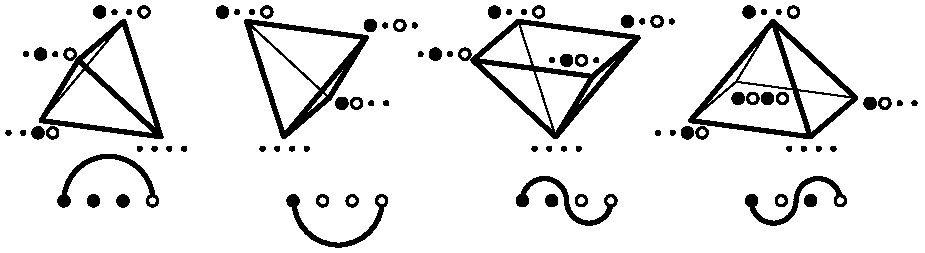
\includegraphics[scale=1]{shardPolytopes}}
	\caption{The shard polytopes of the up arc~$(1, 4, \{2, 3\}, \varnothing)$, down arc~$(1, 4, \varnothing, \{2, 3\})$, yin arc~$(1, 4, \{2\}, \{3\})$, and yang arc~$(1, 4, \{3\}, \{2\})$. The vertices of the shard polytope of an arc~$\alpha \eqdef (a, b, A, B)$ are labeled by the corresponding $\alpha$-alternating matchings, where we use solid dots~$\bullet$ for elements in~$\{a\} \cup A$ and hollow dots~$\circ$ for elements in~$B \cup \{b\}$. The corresponding vertex coordinates are directly read replacing~$\bullet$ by~$1$ and~$\circ$ by~$-1$. For instance, the vertex labeled~${\bullet \cdot \cdot \,\circ}$ has coordinates~$(1,0,0,-1)$. Adapted from~\cite[Fig.~10]{MR4584712}.}
	\label{fig:shardPolytiopes}
\end{figure}

By definition, any quotientope is a deformed permutahedron, and can thus be written as
  \[
  \Bigset{x \in \R^n}{ \sum_{i \in [n]} x_i = f([n]) \text{ and } \sum_{i \in S} x_i \le f(S) \text{ for all } \varnothing \ne S \subseteq [n]},
  \]
where~$f$ is a \defn{submodular} set function $f:2^{[n]}\mapsto \R$ (\ie such that~$f(X \cup Y) + f(X \cap Y) \le f(X) + f(Y)$ for any~$X, Y \subseteq [n]$).
Recall that the submodular function of a Minkowski sum of deformed permutahedra is just the sum of the submodular functions of the Minkowski summands.

\begin{lemma}
  \label{lem:submodsum}
  \vincent{I would not make this one so visible in a proper thm environment.}
  Consider a collection $\polytope{P}_1, \polytope{P}_2,\ldots ,\polytope{P}_k$ of deformed permutahedra defined by the submodular functions $f_1,f_2,\ldots ,f_k$. Then the Minkowski sum $\sum_i \polytope{P}_i$ is defined by the submodular function $f \eqdef \sum_i f_i$.
\end{lemma}

%%%%%%%%%%%%%%%%%%%%%%%%%%%%%%%%%%%%%%
%%%%%%%%%%%%%%%%%%%%%%%%%%%%%%%%%%%%%%

\section{Weak rectangulotopes}
\label{sec:weakRectangulotopes}

%%%%%%%%%%%%%

\subsection{The weak rectangulation congruence}
\label{subsec:weakRectangulationCongruence}

Given a rectangulation~$R$, the source and target trees~$S(R)$ and~$T(R)$ define two partial orders on $[n]$ (the horizontal edges are oriented from left to right and the vertical edges are oriented from bottom to top).
The \defn{weak poset}~$P_w(R)=([n],\prec_w)$ of the rectangulation~$R$ is the transitive closure of the union of the two partial orders defined by the intertwining binary trees~$S(R)$ and~$T(R)$.
These posets were characterized (and called Baxter posets) by E.~Meehan~\cite{MR4014603}.
The weak poset is a two-dimensional lattice, whose minimum is the root of~$S(R)$ and whose maximum is the root of~$T(R)$.
We define the set~$\mathcal{L}(P_w(R))$ as the linear extensions of the weak poset:
\[
\mathcal{L}(P_w(R)) \eqdef \bigset{\pi\in\f{S}_n }{ i\prec_w j\implies \pi^{-1}(i) < \pi^{-1}(j)}.
\]

\begin{theorem}[\cite{MR2871762}]
  The subsets $\mathcal{L}(P_w(R))$ of $\f{S}_n$, for all rectangulations $R$ of size~$n$, 
  are equivalence classes of a congruence relation $\weakeq$ on the weak Bruhat order on $\f{S}_n$.
  Furthermore:
  \begin{itemize}
  \item the congruence classes are one-to-one with weak rectangulations,  
  \item the minimal elements of each congruence class are the twisted Baxter permutations,
  \item the maximal elements are the co-twisted Baxter permutations,
  \item the congruence classes each contain a single Baxter permutation, and are one-to-one with Baxter permutations.
  \end{itemize}
\end{theorem}

We call this congruence the \defn{weak rectangulation congruence} (it is sometimes referred to as the \defn{Baxter congruence}).
The \defn{weak rectangulotope} $\WRP(n)$ is the quotientope of the weak rectangulation congruence $
\weakeq$ on the weak Bruhat order on $\f{S}_n$.

\subsection{Up and down arcs}
\label{subsec:upDownArcs}

\begin{lemma}
The weak rectangulation congruence $
\weakeq$ on $\f{S}_n$ is defined by the arc ideal composed of arcs that do not cross the horizontal line.
\end{lemma}

These arcs can be classified into two families of arcs: the up arcs and the down arcs.
For an interval $I$ of $[n]$ of size at least~$2$, the \defn{up arc}~$\upArc{I}$ (resp.~\defn{down arc}~$\downArc{I}$) is the arc that starts at~$\min(I)$ and ends at~$\max(I)$, and passes above (resp.~below) all remaining elements of~$I$, that is
\begin{align*}
\upArc{I} & \eqdef \big( \min(I), \max(I), I \ssm \{\min(I), \max(I)\}, \varnothing \big) \\
\qquad\text{and}\qquad
\downArc{I} & \eqdef \big( \min(I), \max(I), \varnothing, I \ssm \{\min(I), \max(I)\} \big).
\end{align*}
Note that the basic arc~$(i, i+1, \varnothing, \varnothing)$ is both an up and down arc.

\subsection{Shard polytopes of up and down arcs}
\label{subsec:upDownShardPolytopes}

Therefore, the quotientope is realized by a Minkowski sum of the shard polytopes of the up arcs and the down arcs.
These quotientopes are very basic ones.

\begin{lemma}
  \label{lem:lodaysp}
%  Given an up arc~$\alpha$ defined by an interval $I$, the up shard polytope $\SP(\alpha)$ is a translate of the standard simplex~$\conv \set{ \b{e}_i }{ i\in I }$.
  The up shard polytope $\SP(\upArc{I})$ is a translate of the simplex~$\conv \set{ \b{e}_i }{ i\in I }$.
\end{lemma}

\begin{lemma}
  \label{lem:antilodaysp}
  The down shard polytope $\SP(\downArc{I})$ is a translate of the negative simplex~$\conv \set{ - \b{e}_i }{ i\in I }$.
\end{lemma}

\begin{lemma}
  \label{lem:weakMinkowski}
  The weak rectangulotope $\WRP(n)$ is realized by the Minkowski sum of all up and down shard polytopes.
  In particular, it is the Minkowski sum of two opposite associahedra of J.-L.~Loday~\cite{MR2871762}.
\end{lemma}

%%%%%%%%%%%%%

\subsection{Submodular functions of weak rectangulotopes}
\label{subsec:submodularWeakRectangulotopes}

The description of the weak rectangulotope~$\WRP(n)$ as a Minkowski sum in \cref{lem:weakMinkowski} allows us to easily compute the corresponding submodular function.
\vincent{Say here that all rays are preserved}

\begin{lemma}
  The weak rectangulotope $\WRP(n)$ is realized by the following submodular function:
  \[
  f_{\weakeq}(S) \eqdef \#\bigset{ I\text{ interval of } [n] }{ I \not\subseteq S \text{ and } I \not\subseteq [n]\ssm S }.
  \]
  %that maps $S$ to the number of intervals $I$ of $[n]$ such that $I\cap S\not=\emptyset$ and $I\not\subseteq S$. 
\end{lemma}

\begin{proof}
  The submodular function defining the realization of $\WRP(n)$ is the sum of the submodular functions defining the up and down shard polytope in \cref{lem:lodaysp,lem:antilodaysp}.
  The shard polytope~$\SP(\upArc{I})$ of an up arc~$\upArc{I}$ is given by the submodular function
  \[
  f_{\upArc{I}}(S) \eqdef \llbracket S\cap I\not=\emptyset \rrbracket .
  \]
  (Recall that $\llbracket \varphi\rrbracket$ is equal to 1 if $\varphi$ holds, and 0 otherwise.)
  Similarly, the shard polytope~$\SP(\downArc{I})$ of a down arc~$\downArc{I}$ is given by the submodular function
  \[
  f_{\downArc{I}}(S) \eqdef - \llbracket I\subseteq S \rrbracket .
  \]
  Their sum
  \[
  f_{\weakeq}(S) = \sum_{I\text{ interval of }[n]} f_{\upArc{I}}(S) + f_{\downArc{I}}(S)
  \]
  is therefore exactly the number of intervals of $I$ that intersect $S$ but are not contained in $S$, hence the number of intervals contained neither in~$S$ nor in its complement.
\end{proof}

%%%%%%%%%%%%%

\subsection{Loday coordinates of weak rectangulotopes}
\label{subsec:LodayWeakRectangulotopes}

For every weak rectangulation $R$, we wish to give the coordinates of a point $\b{p}(R)\in\R^n$ such that $\WRP(n)$ is the convex hull of the points~$\b{p}(R)$ for all weak rectangulations~$R$.
Recall that in a Minkowski sum of polytopes, the vertex that is extremal in a generic direction is the sum of the vertices of the summands that are extremal in this direction.
We therefore need to understand which vertices of the translates of the shard polytopes defined in \cref{lem:lodaysp,lem:antilodaysp} are extremal for a direction given by a permutation.

\begin{lemma}
  \label{lem:lodaymax}
  Let $\pi \in \f{S}_n$ and $I$ be an interval of~$[n]$ of size at least~$2$.
  The unique vertex of the up shard polytope~$\SP(\upArc{I})$ (resp.~of the translated down shard polytope~$\SP(\downArc{I})$) that is extreme with respect to the direction $\pi^{-1}$ is $\b{e}_i$, where $i \eqdef \arg\max_{j\in I} \pi^{-1}(j)$ (resp.~where~$i \eqdef \arg\min_{j\in I} \pi^{-1}(j)$).
\end{lemma}

Note that this extremal vertex should only depend on the weak rectangulation congruence class of $\pi$.
This, in passing, gives us an alternative characterization of the weak rectangulation congruence:
$\pi
\weakeq\sigma$ if and only if for any interval $I$ of $[n]$,
%the maximum and the minimum of $\pi^{-1}$ and $\sigma^{-1}$ on $I$ have the same index.
$\arg\max_{j\in I} \pi^{-1}(j)=\arg\max_{j\in I} \sigma^{-1}(j)$, and
$\arg\min_{j\in I} \pi^{-1}(j)=\arg\min_{j\in I} \sigma^{-1}(j)$.

\begin{lemma}
  Let $R$ be a rectangulation of size~$n$, with source and target trees~$S$ and~$T$, and let $\b{p}(R)$ the vertex of $\WRP(n)$ associated with $R$.
  Given $i\in [n]$, the number of up arcs~$\upArc{I}$ such that $\b{e}_i$ is the extremal vertex of $\SP(\upArc{I})$ contributing to~$\b{p}(R)$ is
  \[
  \loday{w}_i =  h^{T}_i\cdot v^{T}_i,
  \]
   where $h^T_i$ and $v^T_i$ denote respectively the number of leaves in the horizontal and vertical subtrees of $i$ in the tree $T$.
\end{lemma}

%%%%%%%%%%%%%%%%%%%%%%%%%%%%%%%%%%%%%%
%%%%%%%%%%%%%%%%%%%%%%%%%%%%%%%%%%%%%%

\section{Strong rectangulotopes}
\label{sec:strongRectangulotopes}

%%%%%%%%%%%%%

\subsection{The strong rectangulation congruence}
\label{subsec:strongRectangulationCongruence}

We define the \defn{strong poset} $P_s(R)=([n],\prec_s)$ of a rectangulation $R$, and $\mathcal{L}(P_s)$ as the set of permutations of $\f{S}_n$ corresponding to linear extensions of $P_s$:
\[
\mathcal{L}(P_s(R)) \eqdef \bigset{\pi\in\f{S}_n }{ i\prec_s j\implies \pi^{-1}(i) < \pi^{-1}(j)}.
\]

\begin{theorem}[\cite{MR2864445,ACFF24}]
  The subsets $\mathcal{L}(P_s(R))$ of $\f{S}_n$, for all rectangulations $R$ of size~$n$, 
  are equivalence classes of a congruence relation $\strongeq$ on the weak Bruhat order on $\f{S}_n$.
    Furthermore:
  \begin{itemize}
  \item the congruence classes are one-to-one with strong rectangulations,  
  \item the minimal elements of each congruence class are the 2-clumped permutations,
  \item the maximal elements are the co-2-clumped permutations.
  \end{itemize}
\end{theorem}

We call the congruence $\strongeq$ the \defn{strong rectangulation congruence}.
The \defn{strong rectangulotope} $\SRP(n)$ is the quotientope of the strong rectangulation congruence~${\strongeq}$.

%%%%%%%%%%%%%

\subsection{Yin and yang arcs}
\label{subsec:yinYangArcs}

\begin{lemma}
  The strong rectangulation congruence $\strongeq$ on $\f{S}_n$ is defined by the arc ideal composed of arcs that cross the horizontal line at most once.
\end{lemma}

We classify the arcs into two families, depending on whether the arcs cross from above or below.
For two consecutive intervals~$I$ and~$J$ of~$[n]$, the \defn{yin arc}~$\yinArc{I}{J}$ (resp.~\defn{yang arc}~$\yangArc{I}{J}$) is the arc starts at~$\min(I)$ and ends at~$\max(J)$, and goes above (resp.~below) the remaining elements of $I$ and below (resp.~above) the remaining elements of $J$, that is,
\begin{align*}
\yinArc{I}{J} & \eqdef \big( \min(I), \max(J), I \ssm \{\min(I)\}, J \ssm \{\max(J)\} \big) \\
\qquad\text{and}\qquad
\yangArc{I}{J} & \eqdef \big( \min(I), \max(J), J \ssm \{\max(J)\}, I \ssm \{\min(I)\} \big).
\end{align*}
Note that all up arcs and down arcs are both yin arcs and yang arcs.

%%%%%%%%%%%%%

\subsection{Shard polytopes of yin and yang arcs}
\label{subsec:yinYangShardPolytopes}

\begin{lemma}
  \label{lem:yinsp}
  The yin shard polytope $\SP(\yinArc{I}{J})$ is $\conv \{\b{0}\} \cup \set{\b{e}_i - \b{e}_j}{i \in I, \; j \in J}$.
\end{lemma}

\begin{lemma}
  \label{lem:yangsp}
  The yang shard polytope $\SP(\yangArc{I}{J})$ is a translate of~$\conv \{\b{0}\} \cup \set{\b{e}_j - \b{e}_i}{i \in I,\; j \in J}$.
\end{lemma}

%Note that yin shard polytopes are translates of the up shard polytopes when $|J|=1$, and of the down shard polytopes when $|I|=1$.
%Similarly, up and down shard polytopes are translates of some yang shard polytopes.

The following is a direct application of the main result of A.~Padrol, V.~Pilaud, and J.~Ritter~\cite{MR4584712}.

\begin{lemma}
  \label{lem:strongMinkowski}
  The strong rectangulotope $\SRP(n)$ is realized by the Minkowski sum of all yin and yang shard polytopes.
\end{lemma}

Since the combinatorial type of a Minkowski sum is invariant to translation of the summands, we can use the polytopes defined in \cref{lem:yinsp,lem:yangsp} as a definition of the yin and yang shard polytopes.
Also note that since the up and down shard polytopes are, up to a translation, both yin and yang, each up and down shard polytope is summed twice in the proposed realization.
This, again, does not change the combinatorial type of the polytope.

\cref{lem:strongMinkowski} gives us an alternative description of $\SRP(n)$ as the sum of two opposite quotientopes defined by the \defn{yin} and \defn{yang congruences} respectively, where the yin congruence is defined by the arc ideal consisting of all yin arcs, and the yang congruence is defined by the yang arcs.

%%%%%%%%%%%%%

\subsection{Submodular functions of strong rectangulotopes}
\label{subsec:submodularStrongRectangulotopes}

The submodular function corresponding to our realization of $\SRP(n)$ can be obtained as before by summing the functions defining the yin and yang shard polytopes in \cref{lem:yinsp,lem:yangsp}.

\begin{lemma}
  The strong rectangulotope $\SRP(n)$ is realized by the following submodular function:
  \[
  f(S) \eqdef \# \bigset{ I, J }{ I \not\subseteq [n] \ssm S \text{ and } J \not\subseteq S } +
  \#\bigset{ I, J }{ I \not\subseteq S \text{ and } J \not\subseteq [n] \ssm S },
  \]
  where $I, J$ are pairs of nonempty consecutive intervals of~$[n]$.
\end{lemma}

\begin{proof}
  The submodular function defining the realization of $\WRP(n)$ is the sum of the submodular functions defining the yin and yang shard polytopes in \cref{lem:yinsp,lem:yangsp}.
  The shard polytope~$\SP(\yinArc{I}{J})$ of a yin arc $\yinArc{I}{J}$ is given by the submodular function
  \[
  f_{\yinArc{I}{J}}(S) \eqdef \llbracket I \not\subseteq [n] \ssm S \text{ and } J \not\subseteq S \rrbracket .
  \]
  (Recall that $\llbracket \varphi\rrbracket$ is equal to 1 if $\varphi$ holds, and 0 otherwise.)
  Similarly, the shard polytope~$\SP(\yangArc{I}{J})$ of a yang arc~$\yangArc{I}{J}$ is given by the submodular function
  \[
  f_{\yangArc{I}{J}}(S) \eqdef \llbracket I \not\subseteq S \text{ and } J \not\subseteq [n] \ssm S \rrbracket .
  \]
  Their sum
  \[
  f_{\strongeq}(S) \eqdef \sum_{I,J} f_{\yinArc{I}{J}}(S) + f_{\yangArc{I}{J}}(S)
  \]
  is therefore as claimed.
\end{proof}

%%%%%%%%%%%%%

\subsection{Loday coordinates of strong rectangulotopes}
\label{subsec:LodayStrongRectangulotopes}

As in \cref{subsec:LodayWeakRectangulotopes}, we need to understand which vertices of the translates of the yin and yang shard polytopes defined in \cref{lem:yinsp,lem:yangsp} are extremal for a direction given by a permutation.

\begin{lemma}
  \label{lem:yinminmax}
  Let $\pi\in\f{S}_n$, let~$I$ and~$J$ be two consecutive intervals of~$[n]$, and let $i \eqdef \arg\max_{k\in I} \pi^{-1}(k)$ and $j \eqdef \arg\min_{k\in J} \pi^{-1}(k)$.
  The unique vertex of the yin shard polytope~$\SP(\yinArc{I}{J})$ that is extreme with respect to the direction $\pi^{-1}$ is $\b{e}_i-\b{e}_j$ if $\pi^{-1}(i)>\pi^{-1}(j)$, and $\b{0}$ otherwise.
\end{lemma}

Note again that by definition, this extremal vertex should only depend on the strong congruence class of $\pi$.

\begin{lemma}
  Let $R$ be a strong rectangulation of size~$n$, let~$S$ and $T$ be its source and target trees, let~$([n],\prec_s)$ be its strong order, and let~$\b{p}(R)$ be the vertex of $\SRP(n)$ corresponding to $R$.
  Given a pair $i,j\in [n]$ with $i<j$, the number of yin arcs $A$ such that $\b{e}_i-\b{e}_j$ is the extremal vertex of $\SP(A)$ contributing to $p(R)$ is
  \[
    h^T_i \cdot cv^{T,S}_{i,j}\cdot h^S_j 
  \]
  if $i\succ_s j$, and $0$ otherwise.
\end{lemma}
\begin{proof}
  \vincent{I still need to work out this proof...}
  Let $\pi$ be the 2-clumped permutation corresponding to $R$, hence the minimal element of $\mathcal{L}(P_s(R))$ in the weak Bruhat order.
  From \cref{lem:yinminmax}, for a pair $i<j \in [n]$, there exists a yin arc $A$ whose shard polytope $\SP(A)$ contributes to $\b{e}_i-\b{e}_j$ only if
  $\pi^{-1}(i)>\pi^{-1}(j)$, hence if $i\succ_s j$.
  Provided this holds, the set of yin arcs $A$ such that $\SP(A)$ contributes to $\b{e}_i-\b{e}_j$ are defined by pairs of contiguous intervals $I,J$ of $[n]$ with $i\in I$, $j\in J$, such that $i$ is the index of the maximum of $\pi^{-1}$ in $I$, and $j$ is the index of the maximum of $\pi^{-1}$ in $J$.
  %$i = \arg\max_{k\in I} \pi^{-1}(k)$ and $j = \arg\min_{k\in J} \pi^{-1}(k)$.
  We claim that the number of choices of the three endpoints defining such a pair of intervals $I$ and $J$ is the product of the
  number of leaves of the subtree of $T(R)$ rooted at $i$, the number of common leaves to the vertical subtrees of $T(R)$ and $S(R)$ rooted
  at $i$ and $j$, respectively, and the number of leaves of the subtree of $S(R)$ rooted at $j$.
\end{proof}

It remains to observe that the only case where this product is nonzero and $i,j$ is not an inversion in $\pi$ is when $i \, \backslash \, j$.

\begin{lemma}
  Let $R$ be a rectangulation of size~$n$, let $S$ and $T$ be its source and target trees, and let~$([n],\prec_s)$ be the associated strong order.
  Given a pair $i,j\in [n]$ such that $i<j$ and $i\prec_s j$, we have
  \[
    cv^{T,S}_{i,j} > 0 \quad \Longrightarrow \quad i \, \backslash \, j.
  \]
\end{lemma}


%%%%%%%%%%%%%%%%%%%%%%%%%%%%%%%%%%%%%%

%\clearpage
\addtocontents{toc}{ \vspace{.1cm} }
\bibliographystyle{alpha}
\bibliography{rectangulotopes}
\label{sec:biblio}

%%%%%%%%%%%%%%%%%%%%%%%%%%%%%%%%%%%%%%
%%%%%%%%%%%%%%%%%%%%%%%%%%%%%%%%%%%%%%

\newpage
\appendix
\section{Material}

Properties/results we may need along the way.

%%%%%%%%%%%%%

\subsection{Twin binary trees.}

\begin{lemma}
The source tree~$S(R)$ and target tree~$T(R)$ are \defn{twin binary trees}, meaning that they satisfy the following equivalent conditions:
\begin{enumerate}[(i)]
\item $S$ and~$T$ admit a common linear extension,
\item for any~$i \in [n-1]$, the node~$i$ is in the left subtree of the node~$i+1$ in~$S$ if and only if the node~$i+1$ is in the right subtree of the node~$i$ in~$R$,
\item for any~$i \in [n-1]$, the $(i+1)$th leaf of~$S$ is a left leaf if and only if the $(i+1)$th leaf of~$R$ is a right leaf.
\end{enumerate}
\end{lemma}

%%%%%%%%%%%%%

\subsection{Properties of diagonal rectangulations.}

We call \defn{diagonal} the segment joining the top left corner to the bottom right corner.
A rectangulation~$R$ is \defn{diagonal} if it satisfies the following equivalent conditions:
\begin{enumerate}[(i)]
\item all rectangles of~$R$ meet the diagonal,
\item the source~$s(r)$ (resp.~target~$t(r)$) of each rectangle~$r$ of~$R$ is below (resp.~above) the diagonal,
\item the source tree~$S(R)$ (resp.~target tree~$T(R)$) remains below (resp.~above) the diagonal,
\item the source tree~$S(R)$ and the target tree~$T(R)$ do not overlap along a segment of~$R$,
\item $R$ avoids the patterns \horizontalPattern{} and \verticalPattern{},
\item the $2$-clumped permutation~$\projDown(R)$ avoids the patterns~$2413$ and~$3412$,
\item the co-$2$-clumped permutation~$\projDown(R)$ avoids the patterns~$2143$ and~$3142$,
\end{enumerate}


\begin{proposition}
The weak rectangulation insertion of any permutation~$\sigma$ of~$[n]$ is given by the rectangles~$[w\ell(i, \sigma), wr(i, \sigma)-1] \times [n-wd(i, \sigma)+1, n-wu(i, \sigma)]$ for~$i \in [n]$ where
\begin{align*}
w\ell(i, \sigma) & \eqdef \max \; \{0\} \cup \set{j}{j < i \text{ and } \sigma^{-1}(j) < \sigma^{-1}(i)} \\
wr(i, \sigma) & \eqdef \min \; \{n+1\} \cup \set{j}{i < j \text{ and } \sigma^{-1}(i) < \sigma^{-1}(j)} \\
wd(i, \sigma) & \eqdef \min \; \{n+1\} \cup \set{j}{i < j \text{ and } \sigma^{-1}(j) < \sigma^{-1}(i)} \\
\text{and} \qquad
wu(i, \sigma) & \eqdef \max \; \{0\} \cup \set{j}{j < i \text{ and } \sigma^{-1}(i) < \sigma^{-1}(j)}.
\end{align*}
\end{proposition}


\Vincent{
Note that there seem to be a canonical integer drawing of~$R$ described as follows.
For vertical segment~$v$ of~$R$, consider the path~$p$ passing through~$v$ with maximal slope.
The abscissa of~$v$ is then the number of rectangle on the left of~$p$ plus the number of \horizontalPattern{} patterns along~$p$ before~$v$ minus the number of \horizontalPattern{} patterns along~$p$ after~$v$.
The ordinate of an horizontal segment~$h$ of~$R$ is defined symmetrically.
}

\begin{comment}
\newpage
\noindent
\begin{tikzpicture}[very thick, scale=.5]
    \draw (0,0) rectangle (1,2);
    \draw (1,0) rectangle (2,2);
    \node at (1,-.5) {12};
\end{tikzpicture}
\quad
\begin{tikzpicture}[very thick, scale=.5]
    \draw (0,1) rectangle (2,2);
    \draw (0,0) rectangle (2,1);
    \node at (1,-.5) {21};
\end{tikzpicture}
\quad

\vspace{1cm}
\noindent
\begin{tikzpicture}[very thick, scale=.5]
    \draw (0,0) rectangle (1,3);
    \draw (1,0) rectangle (2,3);
    \draw (2,0) rectangle (3,3);
    \node at (1.50000000000000,-.5) {123};
\end{tikzpicture}
\quad
\begin{tikzpicture}[very thick, scale=.5]
    \draw (0,0) rectangle (1,3);
    \draw (1,1) rectangle (3,3);
    \draw (1,0) rectangle (3,1);
    \node at (1.50000000000000,-.5) {132};
\end{tikzpicture}
\quad
\begin{tikzpicture}[very thick, scale=.5]
    \draw (0,1) rectangle (1,3);
    \draw (1,1) rectangle (3,3);
    \draw (0,0) rectangle (3,1);
    \node at (1.50000000000000,-.5) {312};
\end{tikzpicture}
\quad
\begin{tikzpicture}[very thick, scale=.5]
    \draw (0,2) rectangle (2,3);
    \draw (0,0) rectangle (2,2);
    \draw (2,0) rectangle (3,3);
    \node at (1.50000000000000,-.5) {213};
\end{tikzpicture}
\quad
\begin{tikzpicture}[very thick, scale=.5]
    \draw (0,2) rectangle (3,3);
    \draw (0,0) rectangle (2,2);
    \draw (2,0) rectangle (3,2);
    \node at (1.50000000000000,-.5) {231};
\end{tikzpicture}
\quad
\begin{tikzpicture}[very thick, scale=.5]
    \draw (0,2) rectangle (3,3);
    \draw (0,1) rectangle (3,2);
    \draw (0,0) rectangle (3,1);
    \node at (1.50000000000000,-.5) {321};
\end{tikzpicture}
\quad

\vspace{1cm}
\noindent
\begin{tikzpicture}[very thick, scale=.5]
    \draw (0,0) rectangle (1,4);
    \draw (1,0) rectangle (2,4);
    \draw (2,0) rectangle (3,4);
    \draw (3,0) rectangle (4,4);
    \node at (2.00000000000000,-.5) {1234};
\end{tikzpicture}
\quad
\begin{tikzpicture}[very thick, scale=.5]
    \draw (0,0) rectangle (1,4);
    \draw (1,0) rectangle (2,4);
    \draw (2,1) rectangle (4,4);
    \draw (2,0) rectangle (4,1);
    \node at (2.00000000000000,-.5) {1243};
\end{tikzpicture}
\quad
\begin{tikzpicture}[very thick, scale=.5]
    \draw (0,0) rectangle (1,4);
    \draw (1,1) rectangle (2,4);
    \draw (2,1) rectangle (4,4);
    \draw (1,0) rectangle (4,1);
    \node at (2.00000000000000,-.5) {1423};
\end{tikzpicture}
\quad
\begin{tikzpicture}[very thick, scale=.5]
    \draw (0,1) rectangle (1,4);
    \draw (1,1) rectangle (2,4);
    \draw (2,1) rectangle (4,4);
    \draw (0,0) rectangle (4,1);
    \node at (2.00000000000000,-.5) {4123};
\end{tikzpicture}
\quad
\begin{tikzpicture}[very thick, scale=.5]
    \draw (0,0) rectangle (1,4);
    \draw (1,2) rectangle (3,4);
    \draw (1,0) rectangle (3,2);
    \draw (3,0) rectangle (4,4);
    \node at (2.00000000000000,-.5) {1324};
\end{tikzpicture}
\quad
\begin{tikzpicture}[very thick, scale=.5]
    \draw (0,0) rectangle (1,4);
    \draw (1,2) rectangle (4,4);
    \draw (1,0) rectangle (3,2);
    \draw (3,0) rectangle (4,2);
    \node at (2.00000000000000,-.5) {1342};
\end{tikzpicture}
\\[.3cm]
\begin{tikzpicture}[very thick, scale=.5]
    \draw (0,0) rectangle (1,4);
    \draw (1,2) rectangle (4,4);
    \draw (1,1) rectangle (4,2);
    \draw (1,0) rectangle (4,1);
    \node at (2.00000000000000,-.5) {1432};
\end{tikzpicture}
\quad
\begin{tikzpicture}[very thick, scale=.5]
    \draw (0,1) rectangle (1,4);
    \draw (1,2) rectangle (4,4);
    \draw (1,1) rectangle (4,2);
    \draw (0,0) rectangle (4,1);
    \node at (2.00000000000000,-.5) {4132};
\end{tikzpicture}
\quad
\begin{tikzpicture}[very thick, scale=.5]
    \draw (0,2) rectangle (1,4);
    \draw (1,2) rectangle (3,4);
    \draw (0,0) rectangle (3,2);
    \draw (3,0) rectangle (4,4);
    \node at (2.00000000000000,-.5) {3124};
\end{tikzpicture}
\quad
\begin{tikzpicture}[very thick, scale=.5]
    \draw (0,2) rectangle (1,4);
    \draw (1,2) rectangle (4,4);
    \draw (0,0) rectangle (3,2);
    \draw (3,0) rectangle (4,2);
    \node at (2.00000000000000,-.5) {3142};
\end{tikzpicture}
\quad
\begin{tikzpicture}[very thick, scale=.5]
    \draw (0,2) rectangle (5/2,4);
    \draw (5/2,2) rectangle (4,4);
    \draw (0,0) rectangle (3/2,2);
    \draw (3/2,0) rectangle (4,2);
    \node at (2.00000000000000,-.5) {3412};
\end{tikzpicture}
\quad
\begin{tikzpicture}[very thick, scale=.5]
    \draw (0,2) rectangle (1,4);
    \draw (1,2) rectangle (4,4);
    \draw (0,1) rectangle (4,2);
    \draw (0,0) rectangle (4,1);
    \node at (2.00000000000000,-.5) {4312};
\end{tikzpicture}
\\[.3cm]
\begin{tikzpicture}[very thick, scale=.5]
    \draw (0,3) rectangle (2,4);
    \draw (0,0) rectangle (2,3);
    \draw (2,0) rectangle (3,4);
    \draw (3,0) rectangle (4,4);
    \node at (2.00000000000000,-.5) {2134};
\end{tikzpicture}
\quad
\begin{tikzpicture}[very thick, scale=.5]
    \draw (0,3/2) rectangle (2,4);
    \draw (0,0) rectangle (2,3/2);
    \draw (2,5/2) rectangle (4,4);
    \draw (2,0) rectangle (4,5/2);
    \node at (2.00000000000000,-.5) {2143};
\end{tikzpicture}
\quad
\begin{tikzpicture}[very thick, scale=.5]
    \draw (0,3) rectangle (2,4);
    \draw (0,0) rectangle (2,3);
    \draw (2,1) rectangle (4,4);
    \draw (2,0) rectangle (4,1);
    \node at (2.00000000000000,-.5) {2413};
\end{tikzpicture}
\quad
\begin{tikzpicture}[very thick, scale=.5]
    \draw (0,3) rectangle (2,4);
    \draw (0,1) rectangle (2,3);
    \draw (2,1) rectangle (4,4);
    \draw (0,0) rectangle (4,1);
    \node at (2.00000000000000,-.5) {4213};
\end{tikzpicture}
\quad
\begin{tikzpicture}[very thick, scale=.5]
    \draw (0,3) rectangle (3,4);
    \draw (0,0) rectangle (2,3);
    \draw (2,0) rectangle (3,3);
    \draw (3,0) rectangle (4,4);
    \node at (2.00000000000000,-.5) {2314};
\end{tikzpicture}
\quad
\begin{tikzpicture}[very thick, scale=.5]
    \draw (0,3) rectangle (4,4);
    \draw (0,0) rectangle (2,3);
    \draw (2,0) rectangle (3,3);
    \draw (3,0) rectangle (4,3);
    \node at (2.00000000000000,-.5) {2341};
\end{tikzpicture}
\\[.3cm]
\begin{tikzpicture}[very thick, scale=.5]
    \draw (0,3) rectangle (4,4);
    \draw (0,0) rectangle (2,3);
    \draw (2,1) rectangle (4,3);
    \draw (2,0) rectangle (4,1);
    \node at (2.00000000000000,-.5) {2431};
\end{tikzpicture}
\quad
\begin{tikzpicture}[very thick, scale=.5]
    \draw (0,3) rectangle (4,4);
    \draw (0,1) rectangle (2,3);
    \draw (2,1) rectangle (4,3);
    \draw (0,0) rectangle (4,1);
    \node at (2.00000000000000,-.5) {4231};
\end{tikzpicture}
\quad
\begin{tikzpicture}[very thick, scale=.5]
    \draw (0,3) rectangle (3,4);
    \draw (0,2) rectangle (3,3);
    \draw (0,0) rectangle (3,2);
    \draw (3,0) rectangle (4,4);
    \node at (2.00000000000000,-.5) {3214};
\end{tikzpicture}
\quad
\begin{tikzpicture}[very thick, scale=.5]
    \draw (0,3) rectangle (4,4);
    \draw (0,2) rectangle (3,3);
    \draw (0,0) rectangle (3,2);
    \draw (3,0) rectangle (4,3);
    \node at (2.00000000000000,-.5) {3241};
\end{tikzpicture}
\quad
\begin{tikzpicture}[very thick, scale=.5]
    \draw (0,3) rectangle (4,4);
    \draw (0,2) rectangle (4,3);
    \draw (0,0) rectangle (3,2);
    \draw (3,0) rectangle (4,2);
    \node at (2.00000000000000,-.5) {3421};
\end{tikzpicture}
\quad
\begin{tikzpicture}[very thick, scale=.5]
    \draw (0,3) rectangle (4,4);
    \draw (0,2) rectangle (4,3);
    \draw (0,1) rectangle (4,2);
    \draw (0,0) rectangle (4,1);
    \node at (2.00000000000000,-.5) {4321};
\end{tikzpicture}
\\[.3cm]

\newpage
\noindent
\begin{tikzpicture}[very thick, scale=.5]
    \draw (0,0) rectangle (1,5);
    \draw (1,0) rectangle (2,5);
    \draw (2,0) rectangle (3,5);
    \draw (3,0) rectangle (4,5);
    \draw (4,0) rectangle (5,5);
    \node at (2.50000000000000,-.5) {12345};
\end{tikzpicture}
\quad
\begin{tikzpicture}[very thick, scale=.5]
    \draw (0,0) rectangle (1,5);
    \draw (1,0) rectangle (2,5);
    \draw (2,0) rectangle (3,5);
    \draw (3,1) rectangle (5,5);
    \draw (3,0) rectangle (5,1);
    \node at (2.50000000000000,-.5) {12354};
\end{tikzpicture}
\quad
\begin{tikzpicture}[very thick, scale=.5]
    \draw (0,0) rectangle (1,5);
    \draw (1,0) rectangle (2,5);
    \draw (2,1) rectangle (3,5);
    \draw (3,1) rectangle (5,5);
    \draw (2,0) rectangle (5,1);
    \node at (2.50000000000000,-.5) {12534};
\end{tikzpicture}
\quad
\begin{tikzpicture}[very thick, scale=.5]
    \draw (0,0) rectangle (1,5);
    \draw (1,1) rectangle (2,5);
    \draw (2,1) rectangle (3,5);
    \draw (3,1) rectangle (5,5);
    \draw (1,0) rectangle (5,1);
    \node at (2.50000000000000,-.5) {15234};
\end{tikzpicture}
\quad
\begin{tikzpicture}[very thick, scale=.5]
    \draw (0,1) rectangle (1,5);
    \draw (1,1) rectangle (2,5);
    \draw (2,1) rectangle (3,5);
    \draw (3,1) rectangle (5,5);
    \draw (0,0) rectangle (5,1);
    \node at (2.50000000000000,-.5) {51234};
\end{tikzpicture}
\quad
\begin{tikzpicture}[very thick, scale=.5]
    \draw (0,0) rectangle (1,5);
    \draw (1,0) rectangle (2,5);
    \draw (2,2) rectangle (4,5);
    \draw (2,0) rectangle (4,2);
    \draw (4,0) rectangle (5,5);
    \node at (2.50000000000000,-.5) {12435};
\end{tikzpicture}
\\[.3cm]
\begin{tikzpicture}[very thick, scale=.5]
    \draw (0,0) rectangle (1,5);
    \draw (1,0) rectangle (2,5);
    \draw (2,2) rectangle (5,5);
    \draw (2,0) rectangle (4,2);
    \draw (4,0) rectangle (5,2);
    \node at (2.50000000000000,-.5) {12453};
\end{tikzpicture}
\quad
\begin{tikzpicture}[very thick, scale=.5]
    \draw (0,0) rectangle (1,5);
    \draw (1,0) rectangle (2,5);
    \draw (2,2) rectangle (5,5);
    \draw (2,1) rectangle (5,2);
    \draw (2,0) rectangle (5,1);
    \node at (2.50000000000000,-.5) {12543};
\end{tikzpicture}
\quad
\begin{tikzpicture}[very thick, scale=.5]
    \draw (0,0) rectangle (1,5);
    \draw (1,1) rectangle (2,5);
    \draw (2,2) rectangle (5,5);
    \draw (2,1) rectangle (5,2);
    \draw (1,0) rectangle (5,1);
    \node at (2.50000000000000,-.5) {15243};
\end{tikzpicture}
\quad
\begin{tikzpicture}[very thick, scale=.5]
    \draw (0,1) rectangle (1,5);
    \draw (1,1) rectangle (2,5);
    \draw (2,2) rectangle (5,5);
    \draw (2,1) rectangle (5,2);
    \draw (0,0) rectangle (5,1);
    \node at (2.50000000000000,-.5) {51243};
\end{tikzpicture}
\quad
\begin{tikzpicture}[very thick, scale=.5]
    \draw (0,0) rectangle (1,5);
    \draw (1,2) rectangle (2,5);
    \draw (2,2) rectangle (4,5);
    \draw (1,0) rectangle (4,2);
    \draw (4,0) rectangle (5,5);
    \node at (2.50000000000000,-.5) {14235};
\end{tikzpicture}
\quad
\begin{tikzpicture}[very thick, scale=.5]
    \draw (0,0) rectangle (1,5);
    \draw (1,2) rectangle (2,5);
    \draw (2,2) rectangle (5,5);
    \draw (1,0) rectangle (4,2);
    \draw (4,0) rectangle (5,2);
    \node at (2.50000000000000,-.5) {14253};
\end{tikzpicture}
\\[.3cm]
\begin{tikzpicture}[very thick, scale=.5]
    \draw (0,0) rectangle (1,5);
    \draw (1,2) rectangle (7/2,5);
    \draw (7/2,2) rectangle (5,5);
    \draw (1,0) rectangle (5/2,2);
    \draw (5/2,0) rectangle (5,2);
    \node at (2.50000000000000,-.5) {14523};
\end{tikzpicture}
\quad
\begin{tikzpicture}[very thick, scale=.5]
    \draw (0,0) rectangle (1,5);
    \draw (1,2) rectangle (2,5);
    \draw (2,2) rectangle (5,5);
    \draw (1,1) rectangle (5,2);
    \draw (1,0) rectangle (5,1);
    \node at (2.50000000000000,-.5) {15423};
\end{tikzpicture}
\quad
\begin{tikzpicture}[very thick, scale=.5]
    \draw (0,1) rectangle (1,5);
    \draw (1,2) rectangle (2,5);
    \draw (2,2) rectangle (5,5);
    \draw (1,1) rectangle (5,2);
    \draw (0,0) rectangle (5,1);
    \node at (2.50000000000000,-.5) {51423};
\end{tikzpicture}
\quad
\begin{tikzpicture}[very thick, scale=.5]
    \draw (0,2) rectangle (1,5);
    \draw (1,2) rectangle (2,5);
    \draw (2,2) rectangle (4,5);
    \draw (0,0) rectangle (4,2);
    \draw (4,0) rectangle (5,5);
    \node at (2.50000000000000,-.5) {41235};
\end{tikzpicture}
\quad
\begin{tikzpicture}[very thick, scale=.5]
    \draw (0,2) rectangle (1,5);
    \draw (1,2) rectangle (2,5);
    \draw (2,2) rectangle (5,5);
    \draw (0,0) rectangle (4,2);
    \draw (4,0) rectangle (5,2);
    \node at (2.50000000000000,-.5) {41253};
\end{tikzpicture}
\quad
\begin{tikzpicture}[very thick, scale=.5]
    \draw (0,2) rectangle (1,5);
    \draw (1,2) rectangle (7/2,5);
    \draw (7/2,2) rectangle (5,5);
    \draw (0,0) rectangle (5/2,2);
    \draw (5/2,0) rectangle (5,2);
    \node at (2.50000000000000,-.5) {41523};
\end{tikzpicture}
\\[.3cm]
\begin{tikzpicture}[very thick, scale=.5]
    \draw (0,2) rectangle (5/2,5);
    \draw (5/2,2) rectangle (7/2,5);
    \draw (7/2,2) rectangle (5,5);
    \draw (0,0) rectangle (3/2,2);
    \draw (3/2,0) rectangle (5,2);
    \node at (2.50000000000000,-.5) {45123};
\end{tikzpicture}
\quad
\begin{tikzpicture}[very thick, scale=.5]
    \draw (0,2) rectangle (1,5);
    \draw (1,2) rectangle (2,5);
    \draw (2,2) rectangle (5,5);
    \draw (0,1) rectangle (5,2);
    \draw (0,0) rectangle (5,1);
    \node at (2.50000000000000,-.5) {54123};
\end{tikzpicture}
\quad
\begin{tikzpicture}[very thick, scale=.5]
    \draw (0,0) rectangle (1,5);
    \draw (1,3) rectangle (3,5);
    \draw (1,0) rectangle (3,3);
    \draw (3,0) rectangle (4,5);
    \draw (4,0) rectangle (5,5);
    \node at (2.50000000000000,-.5) {13245};
\end{tikzpicture}
\quad
\begin{tikzpicture}[very thick, scale=.5]
    \draw (0,0) rectangle (1,5);
    \draw (1,3/2) rectangle (3,5);
    \draw (1,0) rectangle (3,3/2);
    \draw (3,5/2) rectangle (5,5);
    \draw (3,0) rectangle (5,5/2);
    \node at (2.50000000000000,-.5) {13254};
\end{tikzpicture}
\quad
\begin{tikzpicture}[very thick, scale=.5]
    \draw (0,0) rectangle (1,5);
    \draw (1,3) rectangle (3,5);
    \draw (1,0) rectangle (3,3);
    \draw (3,1) rectangle (5,5);
    \draw (3,0) rectangle (5,1);
    \node at (2.50000000000000,-.5) {13524};
\end{tikzpicture}
\quad
\begin{tikzpicture}[very thick, scale=.5]
    \draw (0,0) rectangle (1,5);
    \draw (1,3) rectangle (3,5);
    \draw (1,1) rectangle (3,3);
    \draw (3,1) rectangle (5,5);
    \draw (1,0) rectangle (5,1);
    \node at (2.50000000000000,-.5) {15324};
\end{tikzpicture}
\\[.3cm]
\begin{tikzpicture}[very thick, scale=.5]
    \draw (0,1) rectangle (1,5);
    \draw (1,3) rectangle (3,5);
    \draw (1,1) rectangle (3,3);
    \draw (3,1) rectangle (5,5);
    \draw (0,0) rectangle (5,1);
    \node at (2.50000000000000,-.5) {51324};
\end{tikzpicture}
\quad
\begin{tikzpicture}[very thick, scale=.5]
    \draw (0,0) rectangle (1,5);
    \draw (1,3) rectangle (4,5);
    \draw (1,0) rectangle (3,3);
    \draw (3,0) rectangle (4,3);
    \draw (4,0) rectangle (5,5);
    \node at (2.50000000000000,-.5) {13425};
\end{tikzpicture}
\quad
\begin{tikzpicture}[very thick, scale=.5]
    \draw (0,0) rectangle (1,5);
    \draw (1,3) rectangle (5,5);
    \draw (1,0) rectangle (3,3);
    \draw (3,0) rectangle (4,3);
    \draw (4,0) rectangle (5,3);
    \node at (2.50000000000000,-.5) {13452};
\end{tikzpicture}
\quad
\begin{tikzpicture}[very thick, scale=.5]
    \draw (0,0) rectangle (1,5);
    \draw (1,3) rectangle (5,5);
    \draw (1,0) rectangle (3,3);
    \draw (3,1) rectangle (5,3);
    \draw (3,0) rectangle (5,1);
    \node at (2.50000000000000,-.5) {13542};
\end{tikzpicture}
\quad
\begin{tikzpicture}[very thick, scale=.5]
    \draw (0,0) rectangle (1,5);
    \draw (1,3) rectangle (5,5);
    \draw (1,1) rectangle (3,3);
    \draw (3,1) rectangle (5,3);
    \draw (1,0) rectangle (5,1);
    \node at (2.50000000000000,-.5) {15342};
\end{tikzpicture}
\quad
\begin{tikzpicture}[very thick, scale=.5]
    \draw (0,1) rectangle (1,5);
    \draw (1,3) rectangle (5,5);
    \draw (1,1) rectangle (3,3);
    \draw (3,1) rectangle (5,3);
    \draw (0,0) rectangle (5,1);
    \node at (2.50000000000000,-.5) {51342};
\end{tikzpicture}
\\[.3cm]
\begin{tikzpicture}[very thick, scale=.5]
    \draw (0,0) rectangle (1,5);
    \draw (1,3) rectangle (4,5);
    \draw (1,2) rectangle (4,3);
    \draw (1,0) rectangle (4,2);
    \draw (4,0) rectangle (5,5);
    \node at (2.50000000000000,-.5) {14325};
\end{tikzpicture}
\quad
\begin{tikzpicture}[very thick, scale=.5]
    \draw (0,0) rectangle (1,5);
    \draw (1,3) rectangle (5,5);
    \draw (1,2) rectangle (4,3);
    \draw (1,0) rectangle (4,2);
    \draw (4,0) rectangle (5,3);
    \node at (2.50000000000000,-.5) {14352};
\end{tikzpicture}
\quad
\begin{tikzpicture}[very thick, scale=.5]
    \draw (0,0) rectangle (1,5);
    \draw (1,3) rectangle (5,5);
    \draw (1,2) rectangle (5,3);
    \draw (1,0) rectangle (4,2);
    \draw (4,0) rectangle (5,2);
    \node at (2.50000000000000,-.5) {14532};
\end{tikzpicture}
\quad
\begin{tikzpicture}[very thick, scale=.5]
    \draw (0,0) rectangle (1,5);
    \draw (1,3) rectangle (5,5);
    \draw (1,2) rectangle (5,3);
    \draw (1,1) rectangle (5,2);
    \draw (1,0) rectangle (5,1);
    \node at (2.50000000000000,-.5) {15432};
\end{tikzpicture}
\quad
\begin{tikzpicture}[very thick, scale=.5]
    \draw (0,1) rectangle (1,5);
    \draw (1,3) rectangle (5,5);
    \draw (1,2) rectangle (5,3);
    \draw (1,1) rectangle (5,2);
    \draw (0,0) rectangle (5,1);
    \node at (2.50000000000000,-.5) {51432};
\end{tikzpicture}
\quad
\begin{tikzpicture}[very thick, scale=.5]
    \draw (0,2) rectangle (1,5);
    \draw (1,3) rectangle (4,5);
    \draw (1,2) rectangle (4,3);
    \draw (0,0) rectangle (4,2);
    \draw (4,0) rectangle (5,5);
    \node at (2.50000000000000,-.5) {41325};
\end{tikzpicture}
\\[.3cm]
\begin{tikzpicture}[very thick, scale=.5]
    \draw (0,2) rectangle (1,5);
    \draw (1,3) rectangle (5,5);
    \draw (1,2) rectangle (4,3);
    \draw (0,0) rectangle (4,2);
    \draw (4,0) rectangle (5,3);
    \node at (2.50000000000000,-.5) {41352};
\end{tikzpicture}
\quad
\begin{tikzpicture}[very thick, scale=.5]
    \draw (0,2) rectangle (1,5);
    \draw (1,3) rectangle (5,5);
    \draw (1,2) rectangle (5,3);
    \draw (0,0) rectangle (4,2);
    \draw (4,0) rectangle (5,2);
    \node at (2.50000000000000,-.5) {41532};
\end{tikzpicture}
\quad
\begin{tikzpicture}[very thick, scale=.5]
    \draw (0,2) rectangle (5/2,5);
    \draw (5/2,3) rectangle (5,5);
    \draw (5/2,2) rectangle (5,3);
    \draw (0,0) rectangle (3/2,2);
    \draw (3/2,0) rectangle (5,2);
    \node at (2.50000000000000,-.5) {45132};
\end{tikzpicture}
\quad
\begin{tikzpicture}[very thick, scale=.5]
    \draw (0,2) rectangle (1,5);
    \draw (1,3) rectangle (5,5);
    \draw (1,2) rectangle (5,3);
    \draw (0,1) rectangle (5,2);
    \draw (0,0) rectangle (5,1);
    \node at (2.50000000000000,-.5) {54132};
\end{tikzpicture}
\quad
\begin{tikzpicture}[very thick, scale=.5]
    \draw (0,3) rectangle (1,5);
    \draw (1,3) rectangle (3,5);
    \draw (0,0) rectangle (3,3);
    \draw (3,0) rectangle (4,5);
    \draw (4,0) rectangle (5,5);
    \node at (2.50000000000000,-.5) {31245};
\end{tikzpicture}
\quad
\begin{tikzpicture}[very thick, scale=.5]
    \draw (0,3/2) rectangle (1,5);
    \draw (1,3/2) rectangle (3,5);
    \draw (0,0) rectangle (3,3/2);
    \draw (3,5/2) rectangle (5,5);
    \draw (3,0) rectangle (5,5/2);
    \node at (2.50000000000000,-.5) {31254};
\end{tikzpicture}
\\[.3cm]
\begin{tikzpicture}[very thick, scale=.5]
    \draw (0,3) rectangle (1,5);
    \draw (1,3) rectangle (3,5);
    \draw (0,0) rectangle (3,3);
    \draw (3,1) rectangle (5,5);
    \draw (3,0) rectangle (5,1);
    \node at (2.50000000000000,-.5) {31524};
\end{tikzpicture}
\quad
\begin{tikzpicture}[very thick, scale=.5]
    \draw (0,3) rectangle (1,5);
    \draw (1,3) rectangle (3,5);
    \draw (0,1) rectangle (3,3);
    \draw (3,1) rectangle (5,5);
    \draw (0,0) rectangle (5,1);
    \node at (2.50000000000000,-.5) {53124};
\end{tikzpicture}
\quad
\begin{tikzpicture}[very thick, scale=.5]
    \draw (0,3) rectangle (1,5);
    \draw (1,3) rectangle (4,5);
    \draw (0,0) rectangle (3,3);
    \draw (3,0) rectangle (4,3);
    \draw (4,0) rectangle (5,5);
    \node at (2.50000000000000,-.5) {31425};
\end{tikzpicture}
\quad
\begin{tikzpicture}[very thick, scale=.5]
    \draw (0,3) rectangle (1,5);
    \draw (1,3) rectangle (5,5);
    \draw (0,0) rectangle (3,3);
    \draw (3,0) rectangle (4,3);
    \draw (4,0) rectangle (5,3);
    \node at (2.50000000000000,-.5) {31452};
\end{tikzpicture}
\quad
\begin{tikzpicture}[very thick, scale=.5]
    \draw (0,3) rectangle (1,5);
    \draw (1,3) rectangle (5,5);
    \draw (0,0) rectangle (3,3);
    \draw (3,1) rectangle (5,3);
    \draw (3,0) rectangle (5,1);
    \node at (2.50000000000000,-.5) {31542};
\end{tikzpicture}
\quad
\begin{tikzpicture}[very thick, scale=.5]
    \draw (0,3) rectangle (1,5);
    \draw (1,3) rectangle (5,5);
    \draw (0,1) rectangle (3,3);
    \draw (3,1) rectangle (5,3);
    \draw (0,0) rectangle (5,1);
    \node at (2.50000000000000,-.5) {53142};
\end{tikzpicture}
\\[.3cm]
\begin{tikzpicture}[very thick, scale=.5]
    \draw (0,3) rectangle (5/2,5);
    \draw (5/2,3) rectangle (4,5);
    \draw (0,0) rectangle (3/2,3);
    \draw (3/2,0) rectangle (4,3);
    \draw (4,0) rectangle (5,5);
    \node at (2.50000000000000,-.5) {34125};
\end{tikzpicture}
\quad
\begin{tikzpicture}[very thick, scale=.5]
    \draw (0,3) rectangle (5/2,5);
    \draw (5/2,3) rectangle (5,5);
    \draw (0,0) rectangle (3/2,3);
    \draw (3/2,0) rectangle (4,3);
    \draw (4,0) rectangle (5,3);
    \node at (2.50000000000000,-.5) {34152};
\end{tikzpicture}
\quad
\begin{tikzpicture}[very thick, scale=.5]
    \draw (0,3) rectangle (7/2,5);
    \draw (7/2,3) rectangle (5,5);
    \draw (0,0) rectangle (3/2,3);
    \draw (3/2,0) rectangle (5/2,3);
    \draw (5/2,0) rectangle (5,3);
    \node at (2.50000000000000,-.5) {34512};
\end{tikzpicture}
\quad
\begin{tikzpicture}[very thick, scale=.5]
    \draw (0,3) rectangle (5/2,5);
    \draw (5/2,3) rectangle (5,5);
    \draw (0,0) rectangle (3/2,3);
    \draw (3/2,1) rectangle (5,3);
    \draw (3/2,0) rectangle (5,1);
    \node at (2.50000000000000,-.5) {35412};
\end{tikzpicture}
\quad
\begin{tikzpicture}[very thick, scale=.5]
    \draw (0,3) rectangle (5/2,5);
    \draw (5/2,3) rectangle (5,5);
    \draw (0,1) rectangle (3/2,3);
    \draw (3/2,1) rectangle (5,3);
    \draw (0,0) rectangle (5,1);
    \node at (2.50000000000000,-.5) {53412};
\end{tikzpicture}
\quad
\begin{tikzpicture}[very thick, scale=.5]
    \draw (0,3) rectangle (1,5);
    \draw (1,3) rectangle (4,5);
    \draw (0,2) rectangle (4,3);
    \draw (0,0) rectangle (4,2);
    \draw (4,0) rectangle (5,5);
    \node at (2.50000000000000,-.5) {43125};
\end{tikzpicture}
\\[.3cm]
\begin{tikzpicture}[very thick, scale=.5]
    \draw (0,3) rectangle (1,5);
    \draw (1,3) rectangle (5,5);
    \draw (0,2) rectangle (4,3);
    \draw (0,0) rectangle (4,2);
    \draw (4,0) rectangle (5,3);
    \node at (2.50000000000000,-.5) {43152};
\end{tikzpicture}
\quad
\begin{tikzpicture}[very thick, scale=.5]
    \draw (0,3) rectangle (7/2,5);
    \draw (7/2,3) rectangle (5,5);
    \draw (0,2) rectangle (5/2,3);
    \draw (0,0) rectangle (5/2,2);
    \draw (5/2,0) rectangle (5,3);
    \node at (2.50000000000000,-.5) {43512};
\end{tikzpicture}
\quad
\begin{tikzpicture}[very thick, scale=.5]
    \draw (0,3) rectangle (1,5);
    \draw (1,3) rectangle (5,5);
    \draw (0,2) rectangle (5,3);
    \draw (0,0) rectangle (4,2);
    \draw (4,0) rectangle (5,2);
    \node at (2.50000000000000,-.5) {45312};
\end{tikzpicture}
\quad
\begin{tikzpicture}[very thick, scale=.5]
    \draw (0,3) rectangle (1,5);
    \draw (1,3) rectangle (5,5);
    \draw (0,2) rectangle (5,3);
    \draw (0,1) rectangle (5,2);
    \draw (0,0) rectangle (5,1);
    \node at (2.50000000000000,-.5) {54312};
\end{tikzpicture}
\quad
\begin{tikzpicture}[very thick, scale=.5]
    \draw (0,4) rectangle (2,5);
    \draw (0,0) rectangle (2,4);
    \draw (2,0) rectangle (3,5);
    \draw (3,0) rectangle (4,5);
    \draw (4,0) rectangle (5,5);
    \node at (2.50000000000000,-.5) {21345};
\end{tikzpicture}
\quad
\begin{tikzpicture}[very thick, scale=.5]
    \draw (0,4) rectangle (2,5);
    \draw (0,0) rectangle (2,4);
    \draw (2,0) rectangle (3,5);
    \draw (3,1) rectangle (5,5);
    \draw (3,0) rectangle (5,1);
    \node at (2.50000000000000,-.5) {21354};
\end{tikzpicture}
\\[.3cm]
\begin{tikzpicture}[very thick, scale=.5]
    \draw (0,3/2) rectangle (2,5);
    \draw (0,0) rectangle (2,3/2);
    \draw (2,5/2) rectangle (3,5);
    \draw (3,5/2) rectangle (5,5);
    \draw (2,0) rectangle (5,5/2);
    \node at (2.50000000000000,-.5) {21534};
\end{tikzpicture}
\quad
\begin{tikzpicture}[very thick, scale=.5]
    \draw (0,4) rectangle (2,5);
    \draw (0,0) rectangle (2,4);
    \draw (2,1) rectangle (3,5);
    \draw (3,1) rectangle (5,5);
    \draw (2,0) rectangle (5,1);
    \node at (2.50000000000000,-.5) {25134};
\end{tikzpicture}
\quad
\begin{tikzpicture}[very thick, scale=.5]
    \draw (0,4) rectangle (2,5);
    \draw (0,1) rectangle (2,4);
    \draw (2,1) rectangle (3,5);
    \draw (3,1) rectangle (5,5);
    \draw (0,0) rectangle (5,1);
    \node at (2.50000000000000,-.5) {52134};
\end{tikzpicture}
\quad
\begin{tikzpicture}[very thick, scale=.5]
    \draw (0,5/2) rectangle (2,5);
    \draw (0,0) rectangle (2,5/2);
    \draw (2,7/2) rectangle (4,5);
    \draw (2,0) rectangle (4,7/2);
    \draw (4,0) rectangle (5,5);
    \node at (2.50000000000000,-.5) {21435};
\end{tikzpicture}
\quad
\begin{tikzpicture}[very thick, scale=.5]
    \draw (0,5/2) rectangle (2,5);
    \draw (0,0) rectangle (2,5/2);
    \draw (2,7/2) rectangle (5,5);
    \draw (2,0) rectangle (4,7/2);
    \draw (4,0) rectangle (5,7/2);
    \node at (2.50000000000000,-.5) {21453};
\end{tikzpicture}
\quad
\begin{tikzpicture}[very thick, scale=.5]
    \draw (0,3/2) rectangle (2,5);
    \draw (0,0) rectangle (2,3/2);
    \draw (2,7/2) rectangle (5,5);
    \draw (2,5/2) rectangle (5,7/2);
    \draw (2,0) rectangle (5,5/2);
    \node at (2.50000000000000,-.5) {21543};
\end{tikzpicture}
\\[.3cm]
\begin{tikzpicture}[very thick, scale=.5]
    \draw (0,5/2) rectangle (2,5);
    \draw (0,0) rectangle (2,5/2);
    \draw (2,7/2) rectangle (5,5);
    \draw (2,1) rectangle (5,7/2);
    \draw (2,0) rectangle (5,1);
    \node at (2.50000000000000,-.5) {25143};
\end{tikzpicture}
\quad
\begin{tikzpicture}[very thick, scale=.5]
    \draw (0,5/2) rectangle (2,5);
    \draw (0,1) rectangle (2,5/2);
    \draw (2,7/2) rectangle (5,5);
    \draw (2,1) rectangle (5,7/2);
    \draw (0,0) rectangle (5,1);
    \node at (2.50000000000000,-.5) {52143};
\end{tikzpicture}
\quad
\begin{tikzpicture}[very thick, scale=.5]
    \draw (0,4) rectangle (2,5);
    \draw (0,0) rectangle (2,4);
    \draw (2,2) rectangle (4,5);
    \draw (2,0) rectangle (4,2);
    \draw (4,0) rectangle (5,5);
    \node at (2.50000000000000,-.5) {24135};
\end{tikzpicture}
\quad
\begin{tikzpicture}[very thick, scale=.5]
    \draw (0,4) rectangle (2,5);
    \draw (0,0) rectangle (2,4);
    \draw (2,2) rectangle (5,5);
    \draw (2,0) rectangle (4,2);
    \draw (4,0) rectangle (5,2);
    \node at (2.50000000000000,-.5) {24153};
\end{tikzpicture}
\quad
\begin{tikzpicture}[very thick, scale=.5]
    \draw (0,4) rectangle (2,5);
    \draw (0,0) rectangle (2,4);
    \draw (2,2) rectangle (5,5);
    \draw (2,1) rectangle (5,2);
    \draw (2,0) rectangle (5,1);
    \node at (2.50000000000000,-.5) {25413};
\end{tikzpicture}
\quad
\begin{tikzpicture}[very thick, scale=.5]
    \draw (0,4) rectangle (2,5);
    \draw (0,1) rectangle (2,4);
    \draw (2,2) rectangle (5,5);
    \draw (2,1) rectangle (5,2);
    \draw (0,0) rectangle (5,1);
    \node at (2.50000000000000,-.5) {52413};
\end{tikzpicture}
\\[.3cm]
\begin{tikzpicture}[very thick, scale=.5]
    \draw (0,4) rectangle (2,5);
    \draw (0,2) rectangle (2,4);
    \draw (2,2) rectangle (4,5);
    \draw (0,0) rectangle (4,2);
    \draw (4,0) rectangle (5,5);
    \node at (2.50000000000000,-.5) {42135};
\end{tikzpicture}
\quad
\begin{tikzpicture}[very thick, scale=.5]
    \draw (0,4) rectangle (2,5);
    \draw (0,2) rectangle (2,4);
    \draw (2,2) rectangle (5,5);
    \draw (0,0) rectangle (4,2);
    \draw (4,0) rectangle (5,2);
    \node at (2.50000000000000,-.5) {42153};
\end{tikzpicture}
\quad
\begin{tikzpicture}[very thick, scale=.5]
    \draw (0,4) rectangle (7/2,5);
    \draw (0,2) rectangle (7/2,4);
    \draw (7/2,2) rectangle (5,5);
    \draw (0,0) rectangle (5/2,2);
    \draw (5/2,0) rectangle (5,2);
    \node at (2.50000000000000,-.5) {45213};
\end{tikzpicture}
\quad
\begin{tikzpicture}[very thick, scale=.5]
    \draw (0,4) rectangle (2,5);
    \draw (0,2) rectangle (2,4);
    \draw (2,2) rectangle (5,5);
    \draw (0,1) rectangle (5,2);
    \draw (0,0) rectangle (5,1);
    \node at (2.50000000000000,-.5) {54213};
\end{tikzpicture}
\quad
\begin{tikzpicture}[very thick, scale=.5]
    \draw (0,4) rectangle (3,5);
    \draw (0,0) rectangle (2,4);
    \draw (2,0) rectangle (3,4);
    \draw (3,0) rectangle (4,5);
    \draw (4,0) rectangle (5,5);
    \node at (2.50000000000000,-.5) {23145};
\end{tikzpicture}
\quad
\begin{tikzpicture}[very thick, scale=.5]
    \draw (0,5/2) rectangle (3,5);
    \draw (0,0) rectangle (2,5/2);
    \draw (2,0) rectangle (3,5/2);
    \draw (3,7/2) rectangle (5,5);
    \draw (3,0) rectangle (5,7/2);
    \node at (2.50000000000000,-.5) {23154};
\end{tikzpicture}
\\[.3cm]
\begin{tikzpicture}[very thick, scale=.5]
    \draw (0,4) rectangle (3,5);
    \draw (0,0) rectangle (2,4);
    \draw (2,0) rectangle (3,4);
    \draw (3,1) rectangle (5,5);
    \draw (3,0) rectangle (5,1);
    \node at (2.50000000000000,-.5) {23514};
\end{tikzpicture}
\quad
\begin{tikzpicture}[very thick, scale=.5]
    \draw (0,4) rectangle (3,5);
    \draw (0,0) rectangle (2,4);
    \draw (2,1) rectangle (3,4);
    \draw (3,1) rectangle (5,5);
    \draw (2,0) rectangle (5,1);
    \node at (2.50000000000000,-.5) {25314};
\end{tikzpicture}
\quad
\begin{tikzpicture}[very thick, scale=.5]
    \draw (0,4) rectangle (3,5);
    \draw (0,1) rectangle (2,4);
    \draw (2,1) rectangle (3,4);
    \draw (3,1) rectangle (5,5);
    \draw (0,0) rectangle (5,1);
    \node at (2.50000000000000,-.5) {52314};
\end{tikzpicture}
\quad
\begin{tikzpicture}[very thick, scale=.5]
    \draw (0,4) rectangle (4,5);
    \draw (0,0) rectangle (2,4);
    \draw (2,0) rectangle (3,4);
    \draw (3,0) rectangle (4,4);
    \draw (4,0) rectangle (5,5);
    \node at (2.50000000000000,-.5) {23415};
\end{tikzpicture}
\quad
\begin{tikzpicture}[very thick, scale=.5]
    \draw (0,4) rectangle (5,5);
    \draw (0,0) rectangle (2,4);
    \draw (2,0) rectangle (3,4);
    \draw (3,0) rectangle (4,4);
    \draw (4,0) rectangle (5,4);
    \node at (2.50000000000000,-.5) {23451};
\end{tikzpicture}
\quad
\begin{tikzpicture}[very thick, scale=.5]
    \draw (0,4) rectangle (5,5);
    \draw (0,0) rectangle (2,4);
    \draw (2,0) rectangle (3,4);
    \draw (3,1) rectangle (5,4);
    \draw (3,0) rectangle (5,1);
    \node at (2.50000000000000,-.5) {23541};
\end{tikzpicture}
\\[.3cm]
\begin{tikzpicture}[very thick, scale=.5]
    \draw (0,4) rectangle (5,5);
    \draw (0,0) rectangle (2,4);
    \draw (2,1) rectangle (3,4);
    \draw (3,1) rectangle (5,4);
    \draw (2,0) rectangle (5,1);
    \node at (2.50000000000000,-.5) {25341};
\end{tikzpicture}
\quad
\begin{tikzpicture}[very thick, scale=.5]
    \draw (0,4) rectangle (5,5);
    \draw (0,1) rectangle (2,4);
    \draw (2,1) rectangle (3,4);
    \draw (3,1) rectangle (5,4);
    \draw (0,0) rectangle (5,1);
    \node at (2.50000000000000,-.5) {52341};
\end{tikzpicture}
\quad
\begin{tikzpicture}[very thick, scale=.5]
    \draw (0,4) rectangle (4,5);
    \draw (0,0) rectangle (2,4);
    \draw (2,2) rectangle (4,4);
    \draw (2,0) rectangle (4,2);
    \draw (4,0) rectangle (5,5);
    \node at (2.50000000000000,-.5) {24315};
\end{tikzpicture}
\quad
\begin{tikzpicture}[very thick, scale=.5]
    \draw (0,4) rectangle (5,5);
    \draw (0,0) rectangle (2,4);
    \draw (2,2) rectangle (4,4);
    \draw (2,0) rectangle (4,2);
    \draw (4,0) rectangle (5,4);
    \node at (2.50000000000000,-.5) {24351};
\end{tikzpicture}
\quad
\begin{tikzpicture}[very thick, scale=.5]
    \draw (0,4) rectangle (5,5);
    \draw (0,0) rectangle (2,4);
    \draw (2,2) rectangle (5,4);
    \draw (2,0) rectangle (4,2);
    \draw (4,0) rectangle (5,2);
    \node at (2.50000000000000,-.5) {24531};
\end{tikzpicture}
\quad
\begin{tikzpicture}[very thick, scale=.5]
    \draw (0,4) rectangle (5,5);
    \draw (0,0) rectangle (2,4);
    \draw (2,2) rectangle (5,4);
    \draw (2,1) rectangle (5,2);
    \draw (2,0) rectangle (5,1);
    \node at (2.50000000000000,-.5) {25431};
\end{tikzpicture}
\\[.3cm]
\begin{tikzpicture}[very thick, scale=.5]
    \draw (0,4) rectangle (5,5);
    \draw (0,1) rectangle (2,4);
    \draw (2,2) rectangle (5,4);
    \draw (2,1) rectangle (5,2);
    \draw (0,0) rectangle (5,1);
    \node at (2.50000000000000,-.5) {52431};
\end{tikzpicture}
\quad
\begin{tikzpicture}[very thick, scale=.5]
    \draw (0,4) rectangle (4,5);
    \draw (0,2) rectangle (2,4);
    \draw (2,2) rectangle (4,4);
    \draw (0,0) rectangle (4,2);
    \draw (4,0) rectangle (5,5);
    \node at (2.50000000000000,-.5) {42315};
\end{tikzpicture}
\quad
\begin{tikzpicture}[very thick, scale=.5]
    \draw (0,4) rectangle (5,5);
    \draw (0,2) rectangle (2,4);
    \draw (2,2) rectangle (4,4);
    \draw (0,0) rectangle (4,2);
    \draw (4,0) rectangle (5,4);
    \node at (2.50000000000000,-.5) {42351};
\end{tikzpicture}
\quad
\begin{tikzpicture}[very thick, scale=.5]
    \draw (0,4) rectangle (5,5);
    \draw (0,2) rectangle (2,4);
    \draw (2,2) rectangle (5,4);
    \draw (0,0) rectangle (4,2);
    \draw (4,0) rectangle (5,2);
    \node at (2.50000000000000,-.5) {42531};
\end{tikzpicture}
\quad
\begin{tikzpicture}[very thick, scale=.5]
    \draw (0,4) rectangle (5,5);
    \draw (0,2) rectangle (7/2,4);
    \draw (7/2,2) rectangle (5,4);
    \draw (0,0) rectangle (5/2,2);
    \draw (5/2,0) rectangle (5,2);
    \node at (2.50000000000000,-.5) {45231};
\end{tikzpicture}
\quad
\begin{tikzpicture}[very thick, scale=.5]
    \draw (0,4) rectangle (5,5);
    \draw (0,2) rectangle (2,4);
    \draw (2,2) rectangle (5,4);
    \draw (0,1) rectangle (5,2);
    \draw (0,0) rectangle (5,1);
    \node at (2.50000000000000,-.5) {54231};
\end{tikzpicture}
\\[.3cm]
\begin{tikzpicture}[very thick, scale=.5]
    \draw (0,4) rectangle (3,5);
    \draw (0,3) rectangle (3,4);
    \draw (0,0) rectangle (3,3);
    \draw (3,0) rectangle (4,5);
    \draw (4,0) rectangle (5,5);
    \node at (2.50000000000000,-.5) {32145};
\end{tikzpicture}
\quad
\begin{tikzpicture}[very thick, scale=.5]
    \draw (0,5/2) rectangle (3,5);
    \draw (0,3/2) rectangle (3,5/2);
    \draw (0,0) rectangle (3,3/2);
    \draw (3,7/2) rectangle (5,5);
    \draw (3,0) rectangle (5,7/2);
    \node at (2.50000000000000,-.5) {32154};
\end{tikzpicture}
\quad
\begin{tikzpicture}[very thick, scale=.5]
    \draw (0,4) rectangle (3,5);
    \draw (0,3/2) rectangle (3,4);
    \draw (0,0) rectangle (3,3/2);
    \draw (3,5/2) rectangle (5,5);
    \draw (3,0) rectangle (5,5/2);
    \node at (2.50000000000000,-.5) {32514};
\end{tikzpicture}
\quad
\begin{tikzpicture}[very thick, scale=.5]
    \draw (0,4) rectangle (3,5);
    \draw (0,3) rectangle (3,4);
    \draw (0,0) rectangle (3,3);
    \draw (3,1) rectangle (5,5);
    \draw (3,0) rectangle (5,1);
    \node at (2.50000000000000,-.5) {35214};
\end{tikzpicture}
\quad
\begin{tikzpicture}[very thick, scale=.5]
    \draw (0,4) rectangle (3,5);
    \draw (0,3) rectangle (3,4);
    \draw (0,1) rectangle (3,3);
    \draw (3,1) rectangle (5,5);
    \draw (0,0) rectangle (5,1);
    \node at (2.50000000000000,-.5) {53214};
\end{tikzpicture}
\quad
\begin{tikzpicture}[very thick, scale=.5]
    \draw (0,4) rectangle (4,5);
    \draw (0,3) rectangle (3,4);
    \draw (0,0) rectangle (3,3);
    \draw (3,0) rectangle (4,4);
    \draw (4,0) rectangle (5,5);
    \node at (2.50000000000000,-.5) {32415};
\end{tikzpicture}
\\[.3cm]
\begin{tikzpicture}[very thick, scale=.5]
    \draw (0,4) rectangle (5,5);
    \draw (0,3) rectangle (3,4);
    \draw (0,0) rectangle (3,3);
    \draw (3,0) rectangle (4,4);
    \draw (4,0) rectangle (5,4);
    \node at (2.50000000000000,-.5) {32451};
\end{tikzpicture}
\quad
\begin{tikzpicture}[very thick, scale=.5]
    \draw (0,4) rectangle (5,5);
    \draw (0,3/2) rectangle (3,4);
    \draw (0,0) rectangle (3,3/2);
    \draw (3,5/2) rectangle (5,4);
    \draw (3,0) rectangle (5,5/2);
    \node at (2.50000000000000,-.5) {32541};
\end{tikzpicture}
\quad
\begin{tikzpicture}[very thick, scale=.5]
    \draw (0,4) rectangle (5,5);
    \draw (0,3) rectangle (3,4);
    \draw (0,0) rectangle (3,3);
    \draw (3,1) rectangle (5,4);
    \draw (3,0) rectangle (5,1);
    \node at (2.50000000000000,-.5) {35241};
\end{tikzpicture}
\quad
\begin{tikzpicture}[very thick, scale=.5]
    \draw (0,4) rectangle (5,5);
    \draw (0,3) rectangle (3,4);
    \draw (0,1) rectangle (3,3);
    \draw (3,1) rectangle (5,4);
    \draw (0,0) rectangle (5,1);
    \node at (2.50000000000000,-.5) {53241};
\end{tikzpicture}
\quad
\begin{tikzpicture}[very thick, scale=.5]
    \draw (0,4) rectangle (4,5);
    \draw (0,3) rectangle (4,4);
    \draw (0,0) rectangle (3,3);
    \draw (3,0) rectangle (4,3);
    \draw (4,0) rectangle (5,5);
    \node at (2.50000000000000,-.5) {34215};
\end{tikzpicture}
\quad
\begin{tikzpicture}[very thick, scale=.5]
    \draw (0,4) rectangle (5,5);
    \draw (0,3) rectangle (4,4);
    \draw (0,0) rectangle (3,3);
    \draw (3,0) rectangle (4,3);
    \draw (4,0) rectangle (5,4);
    \node at (2.50000000000000,-.5) {34251};
\end{tikzpicture}
\\[.3cm]
\begin{tikzpicture}[very thick, scale=.5]
    \draw (0,4) rectangle (5,5);
    \draw (0,3) rectangle (5,4);
    \draw (0,0) rectangle (3,3);
    \draw (3,0) rectangle (4,3);
    \draw (4,0) rectangle (5,3);
    \node at (2.50000000000000,-.5) {34521};
\end{tikzpicture}
\quad
\begin{tikzpicture}[very thick, scale=.5]
    \draw (0,4) rectangle (5,5);
    \draw (0,3) rectangle (5,4);
    \draw (0,0) rectangle (3,3);
    \draw (3,1) rectangle (5,3);
    \draw (3,0) rectangle (5,1);
    \node at (2.50000000000000,-.5) {35421};
\end{tikzpicture}
\quad
\begin{tikzpicture}[very thick, scale=.5]
    \draw (0,4) rectangle (5,5);
    \draw (0,3) rectangle (5,4);
    \draw (0,1) rectangle (3,3);
    \draw (3,1) rectangle (5,3);
    \draw (0,0) rectangle (5,1);
    \node at (2.50000000000000,-.5) {53421};
\end{tikzpicture}
\quad
\begin{tikzpicture}[very thick, scale=.5]
    \draw (0,4) rectangle (4,5);
    \draw (0,3) rectangle (4,4);
    \draw (0,2) rectangle (4,3);
    \draw (0,0) rectangle (4,2);
    \draw (4,0) rectangle (5,5);
    \node at (2.50000000000000,-.5) {43215};
\end{tikzpicture}
\quad
\begin{tikzpicture}[very thick, scale=.5]
    \draw (0,4) rectangle (5,5);
    \draw (0,3) rectangle (4,4);
    \draw (0,2) rectangle (4,3);
    \draw (0,0) rectangle (4,2);
    \draw (4,0) rectangle (5,4);
    \node at (2.50000000000000,-.5) {43251};
\end{tikzpicture}
\quad
\begin{tikzpicture}[very thick, scale=.5]
    \draw (0,4) rectangle (5,5);
    \draw (0,3) rectangle (5,4);
    \draw (0,2) rectangle (4,3);
    \draw (0,0) rectangle (4,2);
    \draw (4,0) rectangle (5,3);
    \node at (2.50000000000000,-.5) {43521};
\end{tikzpicture}
\\[.3cm]
\begin{tikzpicture}[very thick, scale=.5]
    \draw (0,4) rectangle (5,5);
    \draw (0,3) rectangle (5,4);
    \draw (0,2) rectangle (5,3);
    \draw (0,0) rectangle (4,2);
    \draw (4,0) rectangle (5,2);
    \node at (2.50000000000000,-.5) {45321};
\end{tikzpicture}
\quad
\begin{tikzpicture}[very thick, scale=.5]
    \draw (0,4) rectangle (5,5);
    \draw (0,3) rectangle (5,4);
    \draw (0,2) rectangle (5,3);
    \draw (0,1) rectangle (5,2);
    \draw (0,0) rectangle (5,1);
    \node at (2.50000000000000,-.5) {54321};
\end{tikzpicture}
\quad

\newpage
\noindent
\begin{tikzpicture}[very thick, scale=.5]
    \draw (0,0) rectangle (1,6);
    \draw (1,0) rectangle (2,6);
    \draw (2,0) rectangle (3,6);
    \draw (3,0) rectangle (4,6);
    \draw (4,0) rectangle (5,6);
    \draw (5,0) rectangle (6,6);
    \node at (3.00000000000000,-.5) {123456};
\end{tikzpicture}
\quad
\begin{tikzpicture}[very thick, scale=.5]
    \draw (0,0) rectangle (1,6);
    \draw (1,0) rectangle (2,6);
    \draw (2,0) rectangle (3,6);
    \draw (3,0) rectangle (4,6);
    \draw (4,1) rectangle (6,6);
    \draw (4,0) rectangle (6,1);
    \node at (3.00000000000000,-.5) {123465};
\end{tikzpicture}
\quad
\begin{tikzpicture}[very thick, scale=.5]
    \draw (0,0) rectangle (1,6);
    \draw (1,0) rectangle (2,6);
    \draw (2,0) rectangle (3,6);
    \draw (3,1) rectangle (4,6);
    \draw (4,1) rectangle (6,6);
    \draw (3,0) rectangle (6,1);
    \node at (3.00000000000000,-.5) {123645};
\end{tikzpicture}
\quad
\begin{tikzpicture}[very thick, scale=.5]
    \draw (0,0) rectangle (1,6);
    \draw (1,0) rectangle (2,6);
    \draw (2,1) rectangle (3,6);
    \draw (3,1) rectangle (4,6);
    \draw (4,1) rectangle (6,6);
    \draw (2,0) rectangle (6,1);
    \node at (3.00000000000000,-.5) {126345};
\end{tikzpicture}
\quad
\begin{tikzpicture}[very thick, scale=.5]
    \draw (0,0) rectangle (1,6);
    \draw (1,1) rectangle (2,6);
    \draw (2,1) rectangle (3,6);
    \draw (3,1) rectangle (4,6);
    \draw (4,1) rectangle (6,6);
    \draw (1,0) rectangle (6,1);
    \node at (3.00000000000000,-.5) {162345};
\end{tikzpicture}
\\[.3cm]
\begin{tikzpicture}[very thick, scale=.5]
    \draw (0,1) rectangle (1,6);
    \draw (1,1) rectangle (2,6);
    \draw (2,1) rectangle (3,6);
    \draw (3,1) rectangle (4,6);
    \draw (4,1) rectangle (6,6);
    \draw (0,0) rectangle (6,1);
    \node at (3.00000000000000,-.5) {612345};
\end{tikzpicture}
\quad
\begin{tikzpicture}[very thick, scale=.5]
    \draw (0,0) rectangle (1,6);
    \draw (1,0) rectangle (2,6);
    \draw (2,0) rectangle (3,6);
    \draw (3,2) rectangle (5,6);
    \draw (3,0) rectangle (5,2);
    \draw (5,0) rectangle (6,6);
    \node at (3.00000000000000,-.5) {123546};
\end{tikzpicture}
\quad
\begin{tikzpicture}[very thick, scale=.5]
    \draw (0,0) rectangle (1,6);
    \draw (1,0) rectangle (2,6);
    \draw (2,0) rectangle (3,6);
    \draw (3,2) rectangle (6,6);
    \draw (3,0) rectangle (5,2);
    \draw (5,0) rectangle (6,2);
    \node at (3.00000000000000,-.5) {123564};
\end{tikzpicture}
\quad
\begin{tikzpicture}[very thick, scale=.5]
    \draw (0,0) rectangle (1,6);
    \draw (1,0) rectangle (2,6);
    \draw (2,0) rectangle (3,6);
    \draw (3,2) rectangle (6,6);
    \draw (3,1) rectangle (6,2);
    \draw (3,0) rectangle (6,1);
    \node at (3.00000000000000,-.5) {123654};
\end{tikzpicture}
\quad
\begin{tikzpicture}[very thick, scale=.5]
    \draw (0,0) rectangle (1,6);
    \draw (1,0) rectangle (2,6);
    \draw (2,1) rectangle (3,6);
    \draw (3,2) rectangle (6,6);
    \draw (3,1) rectangle (6,2);
    \draw (2,0) rectangle (6,1);
    \node at (3.00000000000000,-.5) {126354};
\end{tikzpicture}
\\[.3cm]
\begin{tikzpicture}[very thick, scale=.5]
    \draw (0,0) rectangle (1,6);
    \draw (1,1) rectangle (2,6);
    \draw (2,1) rectangle (3,6);
    \draw (3,2) rectangle (6,6);
    \draw (3,1) rectangle (6,2);
    \draw (1,0) rectangle (6,1);
    \node at (3.00000000000000,-.5) {162354};
\end{tikzpicture}
\quad
\begin{tikzpicture}[very thick, scale=.5]
    \draw (0,1) rectangle (1,6);
    \draw (1,1) rectangle (2,6);
    \draw (2,1) rectangle (3,6);
    \draw (3,2) rectangle (6,6);
    \draw (3,1) rectangle (6,2);
    \draw (0,0) rectangle (6,1);
    \node at (3.00000000000000,-.5) {612354};
\end{tikzpicture}
\quad
\begin{tikzpicture}[very thick, scale=.5]
    \draw (0,0) rectangle (1,6);
    \draw (1,0) rectangle (2,6);
    \draw (2,2) rectangle (3,6);
    \draw (3,2) rectangle (5,6);
    \draw (2,0) rectangle (5,2);
    \draw (5,0) rectangle (6,6);
    \node at (3.00000000000000,-.5) {125346};
\end{tikzpicture}
\quad
\begin{tikzpicture}[very thick, scale=.5]
    \draw (0,0) rectangle (1,6);
    \draw (1,0) rectangle (2,6);
    \draw (2,2) rectangle (3,6);
    \draw (3,2) rectangle (6,6);
    \draw (2,0) rectangle (5,2);
    \draw (5,0) rectangle (6,2);
    \node at (3.00000000000000,-.5) {125364};
\end{tikzpicture}
\quad
\begin{tikzpicture}[very thick, scale=.5]
    \draw (0,0) rectangle (1,6);
    \draw (1,0) rectangle (2,6);
    \draw (2,2) rectangle (9/2,6);
    \draw (9/2,2) rectangle (6,6);
    \draw (2,0) rectangle (7/2,2);
    \draw (7/2,0) rectangle (6,2);
    \node at (3.00000000000000,-.5) {125634};
\end{tikzpicture}
\\[.3cm]
\begin{tikzpicture}[very thick, scale=.5]
    \draw (0,0) rectangle (1,6);
    \draw (1,0) rectangle (2,6);
    \draw (2,2) rectangle (3,6);
    \draw (3,2) rectangle (6,6);
    \draw (2,1) rectangle (6,2);
    \draw (2,0) rectangle (6,1);
    \node at (3.00000000000000,-.5) {126534};
\end{tikzpicture}
\quad
\begin{tikzpicture}[very thick, scale=.5]
    \draw (0,0) rectangle (1,6);
    \draw (1,1) rectangle (2,6);
    \draw (2,2) rectangle (3,6);
    \draw (3,2) rectangle (6,6);
    \draw (2,1) rectangle (6,2);
    \draw (1,0) rectangle (6,1);
    \node at (3.00000000000000,-.5) {162534};
\end{tikzpicture}
\quad
\begin{tikzpicture}[very thick, scale=.5]
    \draw (0,1) rectangle (1,6);
    \draw (1,1) rectangle (2,6);
    \draw (2,2) rectangle (3,6);
    \draw (3,2) rectangle (6,6);
    \draw (2,1) rectangle (6,2);
    \draw (0,0) rectangle (6,1);
    \node at (3.00000000000000,-.5) {612534};
\end{tikzpicture}
\quad
\begin{tikzpicture}[very thick, scale=.5]
    \draw (0,0) rectangle (1,6);
    \draw (1,2) rectangle (2,6);
    \draw (2,2) rectangle (3,6);
    \draw (3,2) rectangle (5,6);
    \draw (1,0) rectangle (5,2);
    \draw (5,0) rectangle (6,6);
    \node at (3.00000000000000,-.5) {152346};
\end{tikzpicture}
\quad
\begin{tikzpicture}[very thick, scale=.5]
    \draw (0,0) rectangle (1,6);
    \draw (1,2) rectangle (2,6);
    \draw (2,2) rectangle (3,6);
    \draw (3,2) rectangle (6,6);
    \draw (1,0) rectangle (5,2);
    \draw (5,0) rectangle (6,2);
    \node at (3.00000000000000,-.5) {152364};
\end{tikzpicture}
\\[.3cm]
\begin{tikzpicture}[very thick, scale=.5]
    \draw (0,0) rectangle (1,6);
    \draw (1,2) rectangle (2,6);
    \draw (2,2) rectangle (9/2,6);
    \draw (9/2,2) rectangle (6,6);
    \draw (1,0) rectangle (7/2,2);
    \draw (7/2,0) rectangle (6,2);
    \node at (3.00000000000000,-.5) {152634};
\end{tikzpicture}
\quad
\begin{tikzpicture}[very thick, scale=.5]
    \draw (0,0) rectangle (1,6);
    \draw (1,2) rectangle (7/2,6);
    \draw (7/2,2) rectangle (9/2,6);
    \draw (9/2,2) rectangle (6,6);
    \draw (1,0) rectangle (5/2,2);
    \draw (5/2,0) rectangle (6,2);
    \node at (3.00000000000000,-.5) {156234};
\end{tikzpicture}
\quad
\begin{tikzpicture}[very thick, scale=.5]
    \draw (0,0) rectangle (1,6);
    \draw (1,2) rectangle (2,6);
    \draw (2,2) rectangle (3,6);
    \draw (3,2) rectangle (6,6);
    \draw (1,1) rectangle (6,2);
    \draw (1,0) rectangle (6,1);
    \node at (3.00000000000000,-.5) {165234};
\end{tikzpicture}
\quad
\begin{tikzpicture}[very thick, scale=.5]
    \draw (0,1) rectangle (1,6);
    \draw (1,2) rectangle (2,6);
    \draw (2,2) rectangle (3,6);
    \draw (3,2) rectangle (6,6);
    \draw (1,1) rectangle (6,2);
    \draw (0,0) rectangle (6,1);
    \node at (3.00000000000000,-.5) {615234};
\end{tikzpicture}
\quad
\begin{tikzpicture}[very thick, scale=.5]
    \draw (0,2) rectangle (1,6);
    \draw (1,2) rectangle (2,6);
    \draw (2,2) rectangle (3,6);
    \draw (3,2) rectangle (5,6);
    \draw (0,0) rectangle (5,2);
    \draw (5,0) rectangle (6,6);
    \node at (3.00000000000000,-.5) {512346};
\end{tikzpicture}
\\[.3cm]
\begin{tikzpicture}[very thick, scale=.5]
    \draw (0,2) rectangle (1,6);
    \draw (1,2) rectangle (2,6);
    \draw (2,2) rectangle (3,6);
    \draw (3,2) rectangle (6,6);
    \draw (0,0) rectangle (5,2);
    \draw (5,0) rectangle (6,2);
    \node at (3.00000000000000,-.5) {512364};
\end{tikzpicture}
\quad
\begin{tikzpicture}[very thick, scale=.5]
    \draw (0,2) rectangle (1,6);
    \draw (1,2) rectangle (2,6);
    \draw (2,2) rectangle (9/2,6);
    \draw (9/2,2) rectangle (6,6);
    \draw (0,0) rectangle (7/2,2);
    \draw (7/2,0) rectangle (6,2);
    \node at (3.00000000000000,-.5) {512634};
\end{tikzpicture}
\quad
\begin{tikzpicture}[very thick, scale=.5]
    \draw (0,2) rectangle (1,6);
    \draw (1,2) rectangle (7/2,6);
    \draw (7/2,2) rectangle (9/2,6);
    \draw (9/2,2) rectangle (6,6);
    \draw (0,0) rectangle (5/2,2);
    \draw (5/2,0) rectangle (6,2);
    \node at (3.00000000000000,-.5) {516234};
\end{tikzpicture}
\quad
\begin{tikzpicture}[very thick, scale=.5]
    \draw (0,2) rectangle (5/2,6);
    \draw (5/2,2) rectangle (7/2,6);
    \draw (7/2,2) rectangle (9/2,6);
    \draw (9/2,2) rectangle (6,6);
    \draw (0,0) rectangle (3/2,2);
    \draw (3/2,0) rectangle (6,2);
    \node at (3.00000000000000,-.5) {561234};
\end{tikzpicture}
\quad
\begin{tikzpicture}[very thick, scale=.5]
    \draw (0,2) rectangle (1,6);
    \draw (1,2) rectangle (2,6);
    \draw (2,2) rectangle (3,6);
    \draw (3,2) rectangle (6,6);
    \draw (0,1) rectangle (6,2);
    \draw (0,0) rectangle (6,1);
    \node at (3.00000000000000,-.5) {651234};
\end{tikzpicture}
\\[.3cm]
\begin{tikzpicture}[very thick, scale=.5]
    \draw (0,0) rectangle (1,6);
    \draw (1,0) rectangle (2,6);
    \draw (2,3) rectangle (4,6);
    \draw (2,0) rectangle (4,3);
    \draw (4,0) rectangle (5,6);
    \draw (5,0) rectangle (6,6);
    \node at (3.00000000000000,-.5) {124356};
\end{tikzpicture}
\quad
\begin{tikzpicture}[very thick, scale=.5]
    \draw (0,0) rectangle (1,6);
    \draw (1,0) rectangle (2,6);
    \draw (2,3/2) rectangle (4,6);
    \draw (2,0) rectangle (4,3/2);
    \draw (4,5/2) rectangle (6,6);
    \draw (4,0) rectangle (6,5/2);
    \node at (3.00000000000000,-.5) {124365};
\end{tikzpicture}
\quad
\begin{tikzpicture}[very thick, scale=.5]
    \draw (0,0) rectangle (1,6);
    \draw (1,0) rectangle (2,6);
    \draw (2,3) rectangle (4,6);
    \draw (2,0) rectangle (4,3);
    \draw (4,1) rectangle (6,6);
    \draw (4,0) rectangle (6,1);
    \node at (3.00000000000000,-.5) {124635};
\end{tikzpicture}
\quad
\begin{tikzpicture}[very thick, scale=.5]
    \draw (0,0) rectangle (1,6);
    \draw (1,0) rectangle (2,6);
    \draw (2,3) rectangle (4,6);
    \draw (2,1) rectangle (4,3);
    \draw (4,1) rectangle (6,6);
    \draw (2,0) rectangle (6,1);
    \node at (3.00000000000000,-.5) {126435};
\end{tikzpicture}
\quad
\begin{tikzpicture}[very thick, scale=.5]
    \draw (0,0) rectangle (1,6);
    \draw (1,1) rectangle (2,6);
    \draw (2,3) rectangle (4,6);
    \draw (2,1) rectangle (4,3);
    \draw (4,1) rectangle (6,6);
    \draw (1,0) rectangle (6,1);
    \node at (3.00000000000000,-.5) {162435};
\end{tikzpicture}
\\[.3cm]
\begin{tikzpicture}[very thick, scale=.5]
    \draw (0,1) rectangle (1,6);
    \draw (1,1) rectangle (2,6);
    \draw (2,3) rectangle (4,6);
    \draw (2,1) rectangle (4,3);
    \draw (4,1) rectangle (6,6);
    \draw (0,0) rectangle (6,1);
    \node at (3.00000000000000,-.5) {612435};
\end{tikzpicture}
\quad
\begin{tikzpicture}[very thick, scale=.5]
    \draw (0,0) rectangle (1,6);
    \draw (1,0) rectangle (2,6);
    \draw (2,3) rectangle (5,6);
    \draw (2,0) rectangle (4,3);
    \draw (4,0) rectangle (5,3);
    \draw (5,0) rectangle (6,6);
    \node at (3.00000000000000,-.5) {124536};
\end{tikzpicture}
\quad
\begin{tikzpicture}[very thick, scale=.5]
    \draw (0,0) rectangle (1,6);
    \draw (1,0) rectangle (2,6);
    \draw (2,3) rectangle (6,6);
    \draw (2,0) rectangle (4,3);
    \draw (4,0) rectangle (5,3);
    \draw (5,0) rectangle (6,3);
    \node at (3.00000000000000,-.5) {124563};
\end{tikzpicture}
\quad
\begin{tikzpicture}[very thick, scale=.5]
    \draw (0,0) rectangle (1,6);
    \draw (1,0) rectangle (2,6);
    \draw (2,3) rectangle (6,6);
    \draw (2,0) rectangle (4,3);
    \draw (4,1) rectangle (6,3);
    \draw (4,0) rectangle (6,1);
    \node at (3.00000000000000,-.5) {124653};
\end{tikzpicture}
\quad
\begin{tikzpicture}[very thick, scale=.5]
    \draw (0,0) rectangle (1,6);
    \draw (1,0) rectangle (2,6);
    \draw (2,3) rectangle (6,6);
    \draw (2,1) rectangle (4,3);
    \draw (4,1) rectangle (6,3);
    \draw (2,0) rectangle (6,1);
    \node at (3.00000000000000,-.5) {126453};
\end{tikzpicture}
\\[.3cm]
\begin{tikzpicture}[very thick, scale=.5]
    \draw (0,0) rectangle (1,6);
    \draw (1,1) rectangle (2,6);
    \draw (2,3) rectangle (6,6);
    \draw (2,1) rectangle (4,3);
    \draw (4,1) rectangle (6,3);
    \draw (1,0) rectangle (6,1);
    \node at (3.00000000000000,-.5) {162453};
\end{tikzpicture}
\quad
\begin{tikzpicture}[very thick, scale=.5]
    \draw (0,1) rectangle (1,6);
    \draw (1,1) rectangle (2,6);
    \draw (2,3) rectangle (6,6);
    \draw (2,1) rectangle (4,3);
    \draw (4,1) rectangle (6,3);
    \draw (0,0) rectangle (6,1);
    \node at (3.00000000000000,-.5) {612453};
\end{tikzpicture}
\quad
\begin{tikzpicture}[very thick, scale=.5]
    \draw (0,0) rectangle (1,6);
    \draw (1,0) rectangle (2,6);
    \draw (2,3) rectangle (5,6);
    \draw (2,2) rectangle (5,3);
    \draw (2,0) rectangle (5,2);
    \draw (5,0) rectangle (6,6);
    \node at (3.00000000000000,-.5) {125436};
\end{tikzpicture}
\quad
\begin{tikzpicture}[very thick, scale=.5]
    \draw (0,0) rectangle (1,6);
    \draw (1,0) rectangle (2,6);
    \draw (2,3) rectangle (6,6);
    \draw (2,2) rectangle (5,3);
    \draw (2,0) rectangle (5,2);
    \draw (5,0) rectangle (6,3);
    \node at (3.00000000000000,-.5) {125463};
\end{tikzpicture}
\quad
\begin{tikzpicture}[very thick, scale=.5]
    \draw (0,0) rectangle (1,6);
    \draw (1,0) rectangle (2,6);
    \draw (2,3) rectangle (6,6);
    \draw (2,2) rectangle (6,3);
    \draw (2,0) rectangle (5,2);
    \draw (5,0) rectangle (6,2);
    \node at (3.00000000000000,-.5) {125643};
\end{tikzpicture}
\\[.3cm]
\begin{tikzpicture}[very thick, scale=.5]
    \draw (0,0) rectangle (1,6);
    \draw (1,0) rectangle (2,6);
    \draw (2,3) rectangle (6,6);
    \draw (2,2) rectangle (6,3);
    \draw (2,1) rectangle (6,2);
    \draw (2,0) rectangle (6,1);
    \node at (3.00000000000000,-.5) {126543};
\end{tikzpicture}
\quad
\begin{tikzpicture}[very thick, scale=.5]
    \draw (0,0) rectangle (1,6);
    \draw (1,1) rectangle (2,6);
    \draw (2,3) rectangle (6,6);
    \draw (2,2) rectangle (6,3);
    \draw (2,1) rectangle (6,2);
    \draw (1,0) rectangle (6,1);
    \node at (3.00000000000000,-.5) {162543};
\end{tikzpicture}
\quad
\begin{tikzpicture}[very thick, scale=.5]
    \draw (0,1) rectangle (1,6);
    \draw (1,1) rectangle (2,6);
    \draw (2,3) rectangle (6,6);
    \draw (2,2) rectangle (6,3);
    \draw (2,1) rectangle (6,2);
    \draw (0,0) rectangle (6,1);
    \node at (3.00000000000000,-.5) {612543};
\end{tikzpicture}
\quad
\begin{tikzpicture}[very thick, scale=.5]
    \draw (0,0) rectangle (1,6);
    \draw (1,2) rectangle (2,6);
    \draw (2,3) rectangle (5,6);
    \draw (2,2) rectangle (5,3);
    \draw (1,0) rectangle (5,2);
    \draw (5,0) rectangle (6,6);
    \node at (3.00000000000000,-.5) {152436};
\end{tikzpicture}
\quad
\begin{tikzpicture}[very thick, scale=.5]
    \draw (0,0) rectangle (1,6);
    \draw (1,2) rectangle (2,6);
    \draw (2,3) rectangle (6,6);
    \draw (2,2) rectangle (5,3);
    \draw (1,0) rectangle (5,2);
    \draw (5,0) rectangle (6,3);
    \node at (3.00000000000000,-.5) {152463};
\end{tikzpicture}
\\[.3cm]
\begin{tikzpicture}[very thick, scale=.5]
    \draw (0,0) rectangle (1,6);
    \draw (1,2) rectangle (2,6);
    \draw (2,3) rectangle (6,6);
    \draw (2,2) rectangle (6,3);
    \draw (1,0) rectangle (5,2);
    \draw (5,0) rectangle (6,2);
    \node at (3.00000000000000,-.5) {152643};
\end{tikzpicture}
\quad
\begin{tikzpicture}[very thick, scale=.5]
    \draw (0,0) rectangle (1,6);
    \draw (1,2) rectangle (7/2,6);
    \draw (7/2,3) rectangle (6,6);
    \draw (7/2,2) rectangle (6,3);
    \draw (1,0) rectangle (5/2,2);
    \draw (5/2,0) rectangle (6,2);
    \node at (3.00000000000000,-.5) {156243};
\end{tikzpicture}
\quad
\begin{tikzpicture}[very thick, scale=.5]
    \draw (0,0) rectangle (1,6);
    \draw (1,2) rectangle (2,6);
    \draw (2,3) rectangle (6,6);
    \draw (2,2) rectangle (6,3);
    \draw (1,1) rectangle (6,2);
    \draw (1,0) rectangle (6,1);
    \node at (3.00000000000000,-.5) {165243};
\end{tikzpicture}
\quad
\begin{tikzpicture}[very thick, scale=.5]
    \draw (0,1) rectangle (1,6);
    \draw (1,2) rectangle (2,6);
    \draw (2,3) rectangle (6,6);
    \draw (2,2) rectangle (6,3);
    \draw (1,1) rectangle (6,2);
    \draw (0,0) rectangle (6,1);
    \node at (3.00000000000000,-.5) {615243};
\end{tikzpicture}
\quad
\begin{tikzpicture}[very thick, scale=.5]
    \draw (0,2) rectangle (1,6);
    \draw (1,2) rectangle (2,6);
    \draw (2,3) rectangle (5,6);
    \draw (2,2) rectangle (5,3);
    \draw (0,0) rectangle (5,2);
    \draw (5,0) rectangle (6,6);
    \node at (3.00000000000000,-.5) {512436};
\end{tikzpicture}
\\[.3cm]
\begin{tikzpicture}[very thick, scale=.5]
    \draw (0,2) rectangle (1,6);
    \draw (1,2) rectangle (2,6);
    \draw (2,3) rectangle (6,6);
    \draw (2,2) rectangle (5,3);
    \draw (0,0) rectangle (5,2);
    \draw (5,0) rectangle (6,3);
    \node at (3.00000000000000,-.5) {512463};
\end{tikzpicture}
\quad
\begin{tikzpicture}[very thick, scale=.5]
    \draw (0,2) rectangle (1,6);
    \draw (1,2) rectangle (2,6);
    \draw (2,3) rectangle (6,6);
    \draw (2,2) rectangle (6,3);
    \draw (0,0) rectangle (5,2);
    \draw (5,0) rectangle (6,2);
    \node at (3.00000000000000,-.5) {512643};
\end{tikzpicture}
\quad
\begin{tikzpicture}[very thick, scale=.5]
    \draw (0,2) rectangle (1,6);
    \draw (1,2) rectangle (7/2,6);
    \draw (7/2,3) rectangle (6,6);
    \draw (7/2,2) rectangle (6,3);
    \draw (0,0) rectangle (5/2,2);
    \draw (5/2,0) rectangle (6,2);
    \node at (3.00000000000000,-.5) {516243};
\end{tikzpicture}
\quad
\begin{tikzpicture}[very thick, scale=.5]
    \draw (0,2) rectangle (5/2,6);
    \draw (5/2,2) rectangle (7/2,6);
    \draw (7/2,3) rectangle (6,6);
    \draw (7/2,2) rectangle (6,3);
    \draw (0,0) rectangle (3/2,2);
    \draw (3/2,0) rectangle (6,2);
    \node at (3.00000000000000,-.5) {561243};
\end{tikzpicture}
\quad
\begin{tikzpicture}[very thick, scale=.5]
    \draw (0,2) rectangle (1,6);
    \draw (1,2) rectangle (2,6);
    \draw (2,3) rectangle (6,6);
    \draw (2,2) rectangle (6,3);
    \draw (0,1) rectangle (6,2);
    \draw (0,0) rectangle (6,1);
    \node at (3.00000000000000,-.5) {651243};
\end{tikzpicture}
\\[.3cm]
\begin{tikzpicture}[very thick, scale=.5]
    \draw (0,0) rectangle (1,6);
    \draw (1,3) rectangle (2,6);
    \draw (2,3) rectangle (4,6);
    \draw (1,0) rectangle (4,3);
    \draw (4,0) rectangle (5,6);
    \draw (5,0) rectangle (6,6);
    \node at (3.00000000000000,-.5) {142356};
\end{tikzpicture}
\quad
\begin{tikzpicture}[very thick, scale=.5]
    \draw (0,0) rectangle (1,6);
    \draw (1,3/2) rectangle (2,6);
    \draw (2,3/2) rectangle (4,6);
    \draw (1,0) rectangle (4,3/2);
    \draw (4,5/2) rectangle (6,6);
    \draw (4,0) rectangle (6,5/2);
    \node at (3.00000000000000,-.5) {142365};
\end{tikzpicture}
\quad
\begin{tikzpicture}[very thick, scale=.5]
    \draw (0,0) rectangle (1,6);
    \draw (1,3) rectangle (2,6);
    \draw (2,3) rectangle (4,6);
    \draw (1,0) rectangle (4,3);
    \draw (4,1) rectangle (6,6);
    \draw (4,0) rectangle (6,1);
    \node at (3.00000000000000,-.5) {142635};
\end{tikzpicture}
\quad
\begin{tikzpicture}[very thick, scale=.5]
    \draw (0,0) rectangle (1,6);
    \draw (1,3) rectangle (2,6);
    \draw (2,3) rectangle (4,6);
    \draw (1,1) rectangle (4,3);
    \draw (4,1) rectangle (6,6);
    \draw (1,0) rectangle (6,1);
    \node at (3.00000000000000,-.5) {164235};
\end{tikzpicture}
\quad
\begin{tikzpicture}[very thick, scale=.5]
    \draw (0,1) rectangle (1,6);
    \draw (1,3) rectangle (2,6);
    \draw (2,3) rectangle (4,6);
    \draw (1,1) rectangle (4,3);
    \draw (4,1) rectangle (6,6);
    \draw (0,0) rectangle (6,1);
    \node at (3.00000000000000,-.5) {614235};
\end{tikzpicture}
\\[.3cm]
\begin{tikzpicture}[very thick, scale=.5]
    \draw (0,0) rectangle (1,6);
    \draw (1,3) rectangle (2,6);
    \draw (2,3) rectangle (5,6);
    \draw (1,0) rectangle (4,3);
    \draw (4,0) rectangle (5,3);
    \draw (5,0) rectangle (6,6);
    \node at (3.00000000000000,-.5) {142536};
\end{tikzpicture}
\quad
\begin{tikzpicture}[very thick, scale=.5]
    \draw (0,0) rectangle (1,6);
    \draw (1,3) rectangle (2,6);
    \draw (2,3) rectangle (6,6);
    \draw (1,0) rectangle (4,3);
    \draw (4,0) rectangle (5,3);
    \draw (5,0) rectangle (6,3);
    \node at (3.00000000000000,-.5) {142563};
\end{tikzpicture}
\quad
\begin{tikzpicture}[very thick, scale=.5]
    \draw (0,0) rectangle (1,6);
    \draw (1,3) rectangle (2,6);
    \draw (2,3) rectangle (6,6);
    \draw (1,0) rectangle (4,3);
    \draw (4,1) rectangle (6,3);
    \draw (4,0) rectangle (6,1);
    \node at (3.00000000000000,-.5) {142653};
\end{tikzpicture}
\quad
\begin{tikzpicture}[very thick, scale=.5]
    \draw (0,0) rectangle (1,6);
    \draw (1,3) rectangle (2,6);
    \draw (2,3) rectangle (6,6);
    \draw (1,1) rectangle (4,3);
    \draw (4,1) rectangle (6,3);
    \draw (1,0) rectangle (6,1);
    \node at (3.00000000000000,-.5) {164253};
\end{tikzpicture}
\quad
\begin{tikzpicture}[very thick, scale=.5]
    \draw (0,1) rectangle (1,6);
    \draw (1,3) rectangle (2,6);
    \draw (2,3) rectangle (6,6);
    \draw (1,1) rectangle (4,3);
    \draw (4,1) rectangle (6,3);
    \draw (0,0) rectangle (6,1);
    \node at (3.00000000000000,-.5) {614253};
\end{tikzpicture}
\\[.3cm]
\begin{tikzpicture}[very thick, scale=.5]
    \draw (0,0) rectangle (1,6);
    \draw (1,3) rectangle (7/2,6);
    \draw (7/2,3) rectangle (5,6);
    \draw (1,0) rectangle (5/2,3);
    \draw (5/2,0) rectangle (5,3);
    \draw (5,0) rectangle (6,6);
    \node at (3.00000000000000,-.5) {145236};
\end{tikzpicture}
\quad
\begin{tikzpicture}[very thick, scale=.5]
    \draw (0,0) rectangle (1,6);
    \draw (1,3) rectangle (7/2,6);
    \draw (7/2,3) rectangle (6,6);
    \draw (1,0) rectangle (5/2,3);
    \draw (5/2,0) rectangle (5,3);
    \draw (5,0) rectangle (6,3);
    \node at (3.00000000000000,-.5) {145263};
\end{tikzpicture}
\quad
\begin{tikzpicture}[very thick, scale=.5]
    \draw (0,0) rectangle (1,6);
    \draw (1,3) rectangle (9/2,6);
    \draw (9/2,3) rectangle (6,6);
    \draw (1,0) rectangle (5/2,3);
    \draw (5/2,0) rectangle (7/2,3);
    \draw (7/2,0) rectangle (6,3);
    \node at (3.00000000000000,-.5) {145623};
\end{tikzpicture}
\quad
\begin{tikzpicture}[very thick, scale=.5]
    \draw (0,0) rectangle (1,6);
    \draw (1,3) rectangle (7/2,6);
    \draw (7/2,3) rectangle (6,6);
    \draw (1,0) rectangle (5/2,3);
    \draw (5/2,1) rectangle (6,3);
    \draw (5/2,0) rectangle (6,1);
    \node at (3.00000000000000,-.5) {146523};
\end{tikzpicture}
\quad
\begin{tikzpicture}[very thick, scale=.5]
    \draw (0,0) rectangle (1,6);
    \draw (1,3) rectangle (7/2,6);
    \draw (7/2,3) rectangle (6,6);
    \draw (1,1) rectangle (5/2,3);
    \draw (5/2,1) rectangle (6,3);
    \draw (1,0) rectangle (6,1);
    \node at (3.00000000000000,-.5) {164523};
\end{tikzpicture}
\\[.3cm]
\begin{tikzpicture}[very thick, scale=.5]
    \draw (0,1) rectangle (1,6);
    \draw (1,3) rectangle (7/2,6);
    \draw (7/2,3) rectangle (6,6);
    \draw (1,1) rectangle (5/2,3);
    \draw (5/2,1) rectangle (6,3);
    \draw (0,0) rectangle (6,1);
    \node at (3.00000000000000,-.5) {614523};
\end{tikzpicture}
\quad
\begin{tikzpicture}[very thick, scale=.5]
    \draw (0,0) rectangle (1,6);
    \draw (1,3) rectangle (2,6);
    \draw (2,3) rectangle (5,6);
    \draw (1,2) rectangle (5,3);
    \draw (1,0) rectangle (5,2);
    \draw (5,0) rectangle (6,6);
    \node at (3.00000000000000,-.5) {154236};
\end{tikzpicture}
\quad
\begin{tikzpicture}[very thick, scale=.5]
    \draw (0,0) rectangle (1,6);
    \draw (1,3) rectangle (2,6);
    \draw (2,3) rectangle (6,6);
    \draw (1,2) rectangle (5,3);
    \draw (1,0) rectangle (5,2);
    \draw (5,0) rectangle (6,3);
    \node at (3.00000000000000,-.5) {154263};
\end{tikzpicture}
\quad
\begin{tikzpicture}[very thick, scale=.5]
    \draw (0,0) rectangle (1,6);
    \draw (1,3) rectangle (9/2,6);
    \draw (9/2,3) rectangle (6,6);
    \draw (1,2) rectangle (7/2,3);
    \draw (1,0) rectangle (7/2,2);
    \draw (7/2,0) rectangle (6,3);
    \node at (3.00000000000000,-.5) {154623};
\end{tikzpicture}
\quad
\begin{tikzpicture}[very thick, scale=.5]
    \draw (0,0) rectangle (1,6);
    \draw (1,3) rectangle (2,6);
    \draw (2,3) rectangle (6,6);
    \draw (1,2) rectangle (6,3);
    \draw (1,0) rectangle (5,2);
    \draw (5,0) rectangle (6,2);
    \node at (3.00000000000000,-.5) {156423};
\end{tikzpicture}
\\[.3cm]
\begin{tikzpicture}[very thick, scale=.5]
    \draw (0,0) rectangle (1,6);
    \draw (1,3) rectangle (2,6);
    \draw (2,3) rectangle (6,6);
    \draw (1,2) rectangle (6,3);
    \draw (1,1) rectangle (6,2);
    \draw (1,0) rectangle (6,1);
    \node at (3.00000000000000,-.5) {165423};
\end{tikzpicture}
\quad
\begin{tikzpicture}[very thick, scale=.5]
    \draw (0,1) rectangle (1,6);
    \draw (1,3) rectangle (2,6);
    \draw (2,3) rectangle (6,6);
    \draw (1,2) rectangle (6,3);
    \draw (1,1) rectangle (6,2);
    \draw (0,0) rectangle (6,1);
    \node at (3.00000000000000,-.5) {615423};
\end{tikzpicture}
\quad
\begin{tikzpicture}[very thick, scale=.5]
    \draw (0,2) rectangle (1,6);
    \draw (1,3) rectangle (2,6);
    \draw (2,3) rectangle (5,6);
    \draw (1,2) rectangle (5,3);
    \draw (0,0) rectangle (5,2);
    \draw (5,0) rectangle (6,6);
    \node at (3.00000000000000,-.5) {514236};
\end{tikzpicture}
\quad
\begin{tikzpicture}[very thick, scale=.5]
    \draw (0,2) rectangle (1,6);
    \draw (1,3) rectangle (2,6);
    \draw (2,3) rectangle (6,6);
    \draw (1,2) rectangle (5,3);
    \draw (0,0) rectangle (5,2);
    \draw (5,0) rectangle (6,3);
    \node at (3.00000000000000,-.5) {514263};
\end{tikzpicture}
\quad
\begin{tikzpicture}[very thick, scale=.5]
    \draw (0,2) rectangle (1,6);
    \draw (1,3) rectangle (9/2,6);
    \draw (9/2,3) rectangle (6,6);
    \draw (1,2) rectangle (7/2,3);
    \draw (0,0) rectangle (7/2,2);
    \draw (7/2,0) rectangle (6,3);
    \node at (3.00000000000000,-.5) {514623};
\end{tikzpicture}
\\[.3cm]
\begin{tikzpicture}[very thick, scale=.5]
    \draw (0,2) rectangle (1,6);
    \draw (1,3) rectangle (2,6);
    \draw (2,3) rectangle (6,6);
    \draw (1,2) rectangle (6,3);
    \draw (0,0) rectangle (5,2);
    \draw (5,0) rectangle (6,2);
    \node at (3.00000000000000,-.5) {516423};
\end{tikzpicture}
\quad
\begin{tikzpicture}[very thick, scale=.5]
    \draw (0,2) rectangle (5/2,6);
    \draw (5/2,3) rectangle (7/2,6);
    \draw (7/2,3) rectangle (6,6);
    \draw (5/2,2) rectangle (6,3);
    \draw (0,0) rectangle (3/2,2);
    \draw (3/2,0) rectangle (6,2);
    \node at (3.00000000000000,-.5) {561423};
\end{tikzpicture}
\quad
\begin{tikzpicture}[very thick, scale=.5]
    \draw (0,2) rectangle (1,6);
    \draw (1,3) rectangle (2,6);
    \draw (2,3) rectangle (6,6);
    \draw (1,2) rectangle (6,3);
    \draw (0,1) rectangle (6,2);
    \draw (0,0) rectangle (6,1);
    \node at (3.00000000000000,-.5) {651423};
\end{tikzpicture}
\quad
\begin{tikzpicture}[very thick, scale=.5]
    \draw (0,3) rectangle (1,6);
    \draw (1,3) rectangle (2,6);
    \draw (2,3) rectangle (4,6);
    \draw (0,0) rectangle (4,3);
    \draw (4,0) rectangle (5,6);
    \draw (5,0) rectangle (6,6);
    \node at (3.00000000000000,-.5) {412356};
\end{tikzpicture}
\quad
\begin{tikzpicture}[very thick, scale=.5]
    \draw (0,3/2) rectangle (1,6);
    \draw (1,3/2) rectangle (2,6);
    \draw (2,3/2) rectangle (4,6);
    \draw (0,0) rectangle (4,3/2);
    \draw (4,5/2) rectangle (6,6);
    \draw (4,0) rectangle (6,5/2);
    \node at (3.00000000000000,-.5) {412365};
\end{tikzpicture}
\\[.3cm]
\begin{tikzpicture}[very thick, scale=.5]
    \draw (0,3) rectangle (1,6);
    \draw (1,3) rectangle (2,6);
    \draw (2,3) rectangle (4,6);
    \draw (0,0) rectangle (4,3);
    \draw (4,1) rectangle (6,6);
    \draw (4,0) rectangle (6,1);
    \node at (3.00000000000000,-.5) {412635};
\end{tikzpicture}
\quad
\begin{tikzpicture}[very thick, scale=.5]
    \draw (0,3) rectangle (1,6);
    \draw (1,3) rectangle (2,6);
    \draw (2,3) rectangle (4,6);
    \draw (0,1) rectangle (4,3);
    \draw (4,1) rectangle (6,6);
    \draw (0,0) rectangle (6,1);
    \node at (3.00000000000000,-.5) {641235};
\end{tikzpicture}
\quad
\begin{tikzpicture}[very thick, scale=.5]
    \draw (0,3) rectangle (1,6);
    \draw (1,3) rectangle (2,6);
    \draw (2,3) rectangle (5,6);
    \draw (0,0) rectangle (4,3);
    \draw (4,0) rectangle (5,3);
    \draw (5,0) rectangle (6,6);
    \node at (3.00000000000000,-.5) {412536};
\end{tikzpicture}
\quad
\begin{tikzpicture}[very thick, scale=.5]
    \draw (0,3) rectangle (1,6);
    \draw (1,3) rectangle (2,6);
    \draw (2,3) rectangle (6,6);
    \draw (0,0) rectangle (4,3);
    \draw (4,0) rectangle (5,3);
    \draw (5,0) rectangle (6,3);
    \node at (3.00000000000000,-.5) {412563};
\end{tikzpicture}
\quad
\begin{tikzpicture}[very thick, scale=.5]
    \draw (0,3) rectangle (1,6);
    \draw (1,3) rectangle (2,6);
    \draw (2,3) rectangle (6,6);
    \draw (0,0) rectangle (4,3);
    \draw (4,1) rectangle (6,3);
    \draw (4,0) rectangle (6,1);
    \node at (3.00000000000000,-.5) {412653};
\end{tikzpicture}
\\[.3cm]
\begin{tikzpicture}[very thick, scale=.5]
    \draw (0,3) rectangle (1,6);
    \draw (1,3) rectangle (2,6);
    \draw (2,3) rectangle (6,6);
    \draw (0,1) rectangle (4,3);
    \draw (4,1) rectangle (6,3);
    \draw (0,0) rectangle (6,1);
    \node at (3.00000000000000,-.5) {641253};
\end{tikzpicture}
\quad
\begin{tikzpicture}[very thick, scale=.5]
    \draw (0,3) rectangle (1,6);
    \draw (1,3) rectangle (7/2,6);
    \draw (7/2,3) rectangle (5,6);
    \draw (0,0) rectangle (5/2,3);
    \draw (5/2,0) rectangle (5,3);
    \draw (5,0) rectangle (6,6);
    \node at (3.00000000000000,-.5) {415236};
\end{tikzpicture}
\quad
\begin{tikzpicture}[very thick, scale=.5]
    \draw (0,3) rectangle (1,6);
    \draw (1,3) rectangle (7/2,6);
    \draw (7/2,3) rectangle (6,6);
    \draw (0,0) rectangle (5/2,3);
    \draw (5/2,0) rectangle (5,3);
    \draw (5,0) rectangle (6,3);
    \node at (3.00000000000000,-.5) {415263};
\end{tikzpicture}
\quad
\begin{tikzpicture}[very thick, scale=.5]
    \draw (0,3) rectangle (1,6);
    \draw (1,3) rectangle (9/2,6);
    \draw (9/2,3) rectangle (6,6);
    \draw (0,0) rectangle (5/2,3);
    \draw (5/2,0) rectangle (7/2,3);
    \draw (7/2,0) rectangle (6,3);
    \node at (3.00000000000000,-.5) {415623};
\end{tikzpicture}
\quad
\begin{tikzpicture}[very thick, scale=.5]
    \draw (0,3) rectangle (1,6);
    \draw (1,3) rectangle (7/2,6);
    \draw (7/2,3) rectangle (6,6);
    \draw (0,0) rectangle (5/2,3);
    \draw (5/2,1) rectangle (6,3);
    \draw (5/2,0) rectangle (6,1);
    \node at (3.00000000000000,-.5) {416523};
\end{tikzpicture}
\\[.3cm]
\begin{tikzpicture}[very thick, scale=.5]
    \draw (0,3) rectangle (1,6);
    \draw (1,3) rectangle (7/2,6);
    \draw (7/2,3) rectangle (6,6);
    \draw (0,1) rectangle (5/2,3);
    \draw (5/2,1) rectangle (6,3);
    \draw (0,0) rectangle (6,1);
    \node at (3.00000000000000,-.5) {641523};
\end{tikzpicture}
\quad
\begin{tikzpicture}[very thick, scale=.5]
    \draw (0,3) rectangle (5/2,6);
    \draw (5/2,3) rectangle (7/2,6);
    \draw (7/2,3) rectangle (5,6);
    \draw (0,0) rectangle (3/2,3);
    \draw (3/2,0) rectangle (5,3);
    \draw (5,0) rectangle (6,6);
    \node at (3.00000000000000,-.5) {451236};
\end{tikzpicture}
\quad
\begin{tikzpicture}[very thick, scale=.5]
    \draw (0,3) rectangle (5/2,6);
    \draw (5/2,3) rectangle (7/2,6);
    \draw (7/2,3) rectangle (6,6);
    \draw (0,0) rectangle (3/2,3);
    \draw (3/2,0) rectangle (5,3);
    \draw (5,0) rectangle (6,3);
    \node at (3.00000000000000,-.5) {451263};
\end{tikzpicture}
\quad
\begin{tikzpicture}[very thick, scale=.5]
    \draw (0,3) rectangle (5/2,6);
    \draw (5/2,3) rectangle (9/2,6);
    \draw (9/2,3) rectangle (6,6);
    \draw (0,0) rectangle (3/2,3);
    \draw (3/2,0) rectangle (7/2,3);
    \draw (7/2,0) rectangle (6,3);
    \node at (3.00000000000000,-.5) {451623};
\end{tikzpicture}
\quad
\begin{tikzpicture}[very thick, scale=.5]
    \draw (0,3) rectangle (7/2,6);
    \draw (7/2,3) rectangle (9/2,6);
    \draw (9/2,3) rectangle (6,6);
    \draw (0,0) rectangle (3/2,3);
    \draw (3/2,0) rectangle (5/2,3);
    \draw (5/2,0) rectangle (6,3);
    \node at (3.00000000000000,-.5) {456123};
\end{tikzpicture}
\\[.3cm]
\begin{tikzpicture}[very thick, scale=.5]
    \draw (0,3) rectangle (5/2,6);
    \draw (5/2,3) rectangle (7/2,6);
    \draw (7/2,3) rectangle (6,6);
    \draw (0,0) rectangle (3/2,3);
    \draw (3/2,1) rectangle (6,3);
    \draw (3/2,0) rectangle (6,1);
    \node at (3.00000000000000,-.5) {465123};
\end{tikzpicture}
\quad
\begin{tikzpicture}[very thick, scale=.5]
    \draw (0,3) rectangle (5/2,6);
    \draw (5/2,3) rectangle (7/2,6);
    \draw (7/2,3) rectangle (6,6);
    \draw (0,1) rectangle (3/2,3);
    \draw (3/2,1) rectangle (6,3);
    \draw (0,0) rectangle (6,1);
    \node at (3.00000000000000,-.5) {645123};
\end{tikzpicture}
\quad
\begin{tikzpicture}[very thick, scale=.5]
    \draw (0,3) rectangle (1,6);
    \draw (1,3) rectangle (2,6);
    \draw (2,3) rectangle (5,6);
    \draw (0,2) rectangle (5,3);
    \draw (0,0) rectangle (5,2);
    \draw (5,0) rectangle (6,6);
    \node at (3.00000000000000,-.5) {541236};
\end{tikzpicture}
\quad
\begin{tikzpicture}[very thick, scale=.5]
    \draw (0,3) rectangle (1,6);
    \draw (1,3) rectangle (2,6);
    \draw (2,3) rectangle (6,6);
    \draw (0,2) rectangle (5,3);
    \draw (0,0) rectangle (5,2);
    \draw (5,0) rectangle (6,3);
    \node at (3.00000000000000,-.5) {541263};
\end{tikzpicture}
\quad
\begin{tikzpicture}[very thick, scale=.5]
    \draw (0,3) rectangle (1,6);
    \draw (1,3) rectangle (9/2,6);
    \draw (9/2,3) rectangle (6,6);
    \draw (0,2) rectangle (7/2,3);
    \draw (0,0) rectangle (7/2,2);
    \draw (7/2,0) rectangle (6,3);
    \node at (3.00000000000000,-.5) {541623};
\end{tikzpicture}
\\[.3cm]
\begin{tikzpicture}[very thick, scale=.5]
    \draw (0,3) rectangle (7/2,6);
    \draw (7/2,3) rectangle (9/2,6);
    \draw (9/2,3) rectangle (6,6);
    \draw (0,2) rectangle (5/2,3);
    \draw (0,0) rectangle (5/2,2);
    \draw (5/2,0) rectangle (6,3);
    \node at (3.00000000000000,-.5) {546123};
\end{tikzpicture}
\quad
\begin{tikzpicture}[very thick, scale=.5]
    \draw (0,3) rectangle (1,6);
    \draw (1,3) rectangle (2,6);
    \draw (2,3) rectangle (6,6);
    \draw (0,2) rectangle (6,3);
    \draw (0,0) rectangle (5,2);
    \draw (5,0) rectangle (6,2);
    \node at (3.00000000000000,-.5) {564123};
\end{tikzpicture}
\quad
\begin{tikzpicture}[very thick, scale=.5]
    \draw (0,3) rectangle (1,6);
    \draw (1,3) rectangle (2,6);
    \draw (2,3) rectangle (6,6);
    \draw (0,2) rectangle (6,3);
    \draw (0,1) rectangle (6,2);
    \draw (0,0) rectangle (6,1);
    \node at (3.00000000000000,-.5) {654123};
\end{tikzpicture}
\quad
\begin{tikzpicture}[very thick, scale=.5]
    \draw (0,0) rectangle (1,6);
    \draw (1,4) rectangle (3,6);
    \draw (1,0) rectangle (3,4);
    \draw (3,0) rectangle (4,6);
    \draw (4,0) rectangle (5,6);
    \draw (5,0) rectangle (6,6);
    \node at (3.00000000000000,-.5) {132456};
\end{tikzpicture}
\quad
\begin{tikzpicture}[very thick, scale=.5]
    \draw (0,0) rectangle (1,6);
    \draw (1,4) rectangle (3,6);
    \draw (1,0) rectangle (3,4);
    \draw (3,0) rectangle (4,6);
    \draw (4,1) rectangle (6,6);
    \draw (4,0) rectangle (6,1);
    \node at (3.00000000000000,-.5) {132465};
\end{tikzpicture}
\\[.3cm]
\begin{tikzpicture}[very thick, scale=.5]
    \draw (0,0) rectangle (1,6);
    \draw (1,3/2) rectangle (3,6);
    \draw (1,0) rectangle (3,3/2);
    \draw (3,5/2) rectangle (4,6);
    \draw (4,5/2) rectangle (6,6);
    \draw (3,0) rectangle (6,5/2);
    \node at (3.00000000000000,-.5) {132645};
\end{tikzpicture}
\quad
\begin{tikzpicture}[very thick, scale=.5]
    \draw (0,0) rectangle (1,6);
    \draw (1,4) rectangle (3,6);
    \draw (1,0) rectangle (3,4);
    \draw (3,1) rectangle (4,6);
    \draw (4,1) rectangle (6,6);
    \draw (3,0) rectangle (6,1);
    \node at (3.00000000000000,-.5) {136245};
\end{tikzpicture}
\quad
\begin{tikzpicture}[very thick, scale=.5]
    \draw (0,0) rectangle (1,6);
    \draw (1,4) rectangle (3,6);
    \draw (1,1) rectangle (3,4);
    \draw (3,1) rectangle (4,6);
    \draw (4,1) rectangle (6,6);
    \draw (1,0) rectangle (6,1);
    \node at (3.00000000000000,-.5) {163245};
\end{tikzpicture}
\quad
\begin{tikzpicture}[very thick, scale=.5]
    \draw (0,1) rectangle (1,6);
    \draw (1,4) rectangle (3,6);
    \draw (1,1) rectangle (3,4);
    \draw (3,1) rectangle (4,6);
    \draw (4,1) rectangle (6,6);
    \draw (0,0) rectangle (6,1);
    \node at (3.00000000000000,-.5) {613245};
\end{tikzpicture}
\quad
\begin{tikzpicture}[very thick, scale=.5]
    \draw (0,0) rectangle (1,6);
    \draw (1,5/2) rectangle (3,6);
    \draw (1,0) rectangle (3,5/2);
    \draw (3,7/2) rectangle (5,6);
    \draw (3,0) rectangle (5,7/2);
    \draw (5,0) rectangle (6,6);
    \node at (3.00000000000000,-.5) {132546};
\end{tikzpicture}
\\[.3cm]
\begin{tikzpicture}[very thick, scale=.5]
    \draw (0,0) rectangle (1,6);
    \draw (1,5/2) rectangle (3,6);
    \draw (1,0) rectangle (3,5/2);
    \draw (3,7/2) rectangle (6,6);
    \draw (3,0) rectangle (5,7/2);
    \draw (5,0) rectangle (6,7/2);
    \node at (3.00000000000000,-.5) {132564};
\end{tikzpicture}
\quad
\begin{tikzpicture}[very thick, scale=.5]
    \draw (0,0) rectangle (1,6);
    \draw (1,3/2) rectangle (3,6);
    \draw (1,0) rectangle (3,3/2);
    \draw (3,7/2) rectangle (6,6);
    \draw (3,5/2) rectangle (6,7/2);
    \draw (3,0) rectangle (6,5/2);
    \node at (3.00000000000000,-.5) {132654};
\end{tikzpicture}
\quad
\begin{tikzpicture}[very thick, scale=.5]
    \draw (0,0) rectangle (1,6);
    \draw (1,5/2) rectangle (3,6);
    \draw (1,0) rectangle (3,5/2);
    \draw (3,7/2) rectangle (6,6);
    \draw (3,1) rectangle (6,7/2);
    \draw (3,0) rectangle (6,1);
    \node at (3.00000000000000,-.5) {136254};
\end{tikzpicture}
\quad
\begin{tikzpicture}[very thick, scale=.5]
    \draw (0,0) rectangle (1,6);
    \draw (1,5/2) rectangle (3,6);
    \draw (1,1) rectangle (3,5/2);
    \draw (3,7/2) rectangle (6,6);
    \draw (3,1) rectangle (6,7/2);
    \draw (1,0) rectangle (6,1);
    \node at (3.00000000000000,-.5) {163254};
\end{tikzpicture}
\quad
\begin{tikzpicture}[very thick, scale=.5]
    \draw (0,1) rectangle (1,6);
    \draw (1,5/2) rectangle (3,6);
    \draw (1,1) rectangle (3,5/2);
    \draw (3,7/2) rectangle (6,6);
    \draw (3,1) rectangle (6,7/2);
    \draw (0,0) rectangle (6,1);
    \node at (3.00000000000000,-.5) {613254};
\end{tikzpicture}
\\[.3cm]
\begin{tikzpicture}[very thick, scale=.5]
    \draw (0,0) rectangle (1,6);
    \draw (1,4) rectangle (3,6);
    \draw (1,0) rectangle (3,4);
    \draw (3,2) rectangle (5,6);
    \draw (3,0) rectangle (5,2);
    \draw (5,0) rectangle (6,6);
    \node at (3.00000000000000,-.5) {135246};
\end{tikzpicture}
\quad
\begin{tikzpicture}[very thick, scale=.5]
    \draw (0,0) rectangle (1,6);
    \draw (1,4) rectangle (3,6);
    \draw (1,0) rectangle (3,4);
    \draw (3,2) rectangle (6,6);
    \draw (3,0) rectangle (5,2);
    \draw (5,0) rectangle (6,2);
    \node at (3.00000000000000,-.5) {135264};
\end{tikzpicture}
\quad
\begin{tikzpicture}[very thick, scale=.5]
    \draw (0,0) rectangle (1,6);
    \draw (1,4) rectangle (3,6);
    \draw (1,0) rectangle (3,4);
    \draw (3,2) rectangle (6,6);
    \draw (3,1) rectangle (6,2);
    \draw (3,0) rectangle (6,1);
    \node at (3.00000000000000,-.5) {136524};
\end{tikzpicture}
\quad
\begin{tikzpicture}[very thick, scale=.5]
    \draw (0,0) rectangle (1,6);
    \draw (1,4) rectangle (3,6);
    \draw (1,1) rectangle (3,4);
    \draw (3,2) rectangle (6,6);
    \draw (3,1) rectangle (6,2);
    \draw (1,0) rectangle (6,1);
    \node at (3.00000000000000,-.5) {163524};
\end{tikzpicture}
\quad
\begin{tikzpicture}[very thick, scale=.5]
    \draw (0,1) rectangle (1,6);
    \draw (1,4) rectangle (3,6);
    \draw (1,1) rectangle (3,4);
    \draw (3,2) rectangle (6,6);
    \draw (3,1) rectangle (6,2);
    \draw (0,0) rectangle (6,1);
    \node at (3.00000000000000,-.5) {613524};
\end{tikzpicture}
\\[.3cm]
\begin{tikzpicture}[very thick, scale=.5]
    \draw (0,0) rectangle (1,6);
    \draw (1,4) rectangle (3,6);
    \draw (1,2) rectangle (3,4);
    \draw (3,2) rectangle (5,6);
    \draw (1,0) rectangle (5,2);
    \draw (5,0) rectangle (6,6);
    \node at (3.00000000000000,-.5) {153246};
\end{tikzpicture}
\quad
\begin{tikzpicture}[very thick, scale=.5]
    \draw (0,0) rectangle (1,6);
    \draw (1,4) rectangle (3,6);
    \draw (1,2) rectangle (3,4);
    \draw (3,2) rectangle (6,6);
    \draw (1,0) rectangle (5,2);
    \draw (5,0) rectangle (6,2);
    \node at (3.00000000000000,-.5) {153264};
\end{tikzpicture}
\quad
\begin{tikzpicture}[very thick, scale=.5]
    \draw (0,0) rectangle (1,6);
    \draw (1,4) rectangle (9/2,6);
    \draw (1,2) rectangle (9/2,4);
    \draw (9/2,2) rectangle (6,6);
    \draw (1,0) rectangle (7/2,2);
    \draw (7/2,0) rectangle (6,2);
    \node at (3.00000000000000,-.5) {156324};
\end{tikzpicture}
\quad
\begin{tikzpicture}[very thick, scale=.5]
    \draw (0,0) rectangle (1,6);
    \draw (1,4) rectangle (3,6);
    \draw (1,2) rectangle (3,4);
    \draw (3,2) rectangle (6,6);
    \draw (1,1) rectangle (6,2);
    \draw (1,0) rectangle (6,1);
    \node at (3.00000000000000,-.5) {165324};
\end{tikzpicture}
\quad
\begin{tikzpicture}[very thick, scale=.5]
    \draw (0,1) rectangle (1,6);
    \draw (1,4) rectangle (3,6);
    \draw (1,2) rectangle (3,4);
    \draw (3,2) rectangle (6,6);
    \draw (1,1) rectangle (6,2);
    \draw (0,0) rectangle (6,1);
    \node at (3.00000000000000,-.5) {615324};
\end{tikzpicture}
\\[.3cm]
\begin{tikzpicture}[very thick, scale=.5]
    \draw (0,2) rectangle (1,6);
    \draw (1,4) rectangle (3,6);
    \draw (1,2) rectangle (3,4);
    \draw (3,2) rectangle (5,6);
    \draw (0,0) rectangle (5,2);
    \draw (5,0) rectangle (6,6);
    \node at (3.00000000000000,-.5) {513246};
\end{tikzpicture}
\quad
\begin{tikzpicture}[very thick, scale=.5]
    \draw (0,2) rectangle (1,6);
    \draw (1,4) rectangle (3,6);
    \draw (1,2) rectangle (3,4);
    \draw (3,2) rectangle (6,6);
    \draw (0,0) rectangle (5,2);
    \draw (5,0) rectangle (6,2);
    \node at (3.00000000000000,-.5) {513264};
\end{tikzpicture}
\quad
\begin{tikzpicture}[very thick, scale=.5]
    \draw (0,2) rectangle (1,6);
    \draw (1,4) rectangle (9/2,6);
    \draw (1,2) rectangle (9/2,4);
    \draw (9/2,2) rectangle (6,6);
    \draw (0,0) rectangle (7/2,2);
    \draw (7/2,0) rectangle (6,2);
    \node at (3.00000000000000,-.5) {516324};
\end{tikzpicture}
\quad
\begin{tikzpicture}[very thick, scale=.5]
    \draw (0,2) rectangle (5/2,6);
    \draw (5/2,4) rectangle (9/2,6);
    \draw (5/2,2) rectangle (9/2,4);
    \draw (9/2,2) rectangle (6,6);
    \draw (0,0) rectangle (3/2,2);
    \draw (3/2,0) rectangle (6,2);
    \node at (3.00000000000000,-.5) {561324};
\end{tikzpicture}
\quad
\begin{tikzpicture}[very thick, scale=.5]
    \draw (0,2) rectangle (1,6);
    \draw (1,4) rectangle (3,6);
    \draw (1,2) rectangle (3,4);
    \draw (3,2) rectangle (6,6);
    \draw (0,1) rectangle (6,2);
    \draw (0,0) rectangle (6,1);
    \node at (3.00000000000000,-.5) {651324};
\end{tikzpicture}
\\[.3cm]
\begin{tikzpicture}[very thick, scale=.5]
    \draw (0,0) rectangle (1,6);
    \draw (1,4) rectangle (4,6);
    \draw (1,0) rectangle (3,4);
    \draw (3,0) rectangle (4,4);
    \draw (4,0) rectangle (5,6);
    \draw (5,0) rectangle (6,6);
    \node at (3.00000000000000,-.5) {134256};
\end{tikzpicture}
\quad
\begin{tikzpicture}[very thick, scale=.5]
    \draw (0,0) rectangle (1,6);
    \draw (1,5/2) rectangle (4,6);
    \draw (1,0) rectangle (3,5/2);
    \draw (3,0) rectangle (4,5/2);
    \draw (4,7/2) rectangle (6,6);
    \draw (4,0) rectangle (6,7/2);
    \node at (3.00000000000000,-.5) {134265};
\end{tikzpicture}
\quad
\begin{tikzpicture}[very thick, scale=.5]
    \draw (0,0) rectangle (1,6);
    \draw (1,4) rectangle (4,6);
    \draw (1,0) rectangle (3,4);
    \draw (3,0) rectangle (4,4);
    \draw (4,1) rectangle (6,6);
    \draw (4,0) rectangle (6,1);
    \node at (3.00000000000000,-.5) {134625};
\end{tikzpicture}
\quad
\begin{tikzpicture}[very thick, scale=.5]
    \draw (0,0) rectangle (1,6);
    \draw (1,4) rectangle (4,6);
    \draw (1,0) rectangle (3,4);
    \draw (3,1) rectangle (4,4);
    \draw (4,1) rectangle (6,6);
    \draw (3,0) rectangle (6,1);
    \node at (3.00000000000000,-.5) {136425};
\end{tikzpicture}
\quad
\begin{tikzpicture}[very thick, scale=.5]
    \draw (0,0) rectangle (1,6);
    \draw (1,4) rectangle (4,6);
    \draw (1,1) rectangle (3,4);
    \draw (3,1) rectangle (4,4);
    \draw (4,1) rectangle (6,6);
    \draw (1,0) rectangle (6,1);
    \node at (3.00000000000000,-.5) {163425};
\end{tikzpicture}
\\[.3cm]
\begin{tikzpicture}[very thick, scale=.5]
    \draw (0,1) rectangle (1,6);
    \draw (1,4) rectangle (4,6);
    \draw (1,1) rectangle (3,4);
    \draw (3,1) rectangle (4,4);
    \draw (4,1) rectangle (6,6);
    \draw (0,0) rectangle (6,1);
    \node at (3.00000000000000,-.5) {613425};
\end{tikzpicture}
\quad
\begin{tikzpicture}[very thick, scale=.5]
    \draw (0,0) rectangle (1,6);
    \draw (1,4) rectangle (5,6);
    \draw (1,0) rectangle (3,4);
    \draw (3,0) rectangle (4,4);
    \draw (4,0) rectangle (5,4);
    \draw (5,0) rectangle (6,6);
    \node at (3.00000000000000,-.5) {134526};
\end{tikzpicture}
\quad
\begin{tikzpicture}[very thick, scale=.5]
    \draw (0,0) rectangle (1,6);
    \draw (1,4) rectangle (6,6);
    \draw (1,0) rectangle (3,4);
    \draw (3,0) rectangle (4,4);
    \draw (4,0) rectangle (5,4);
    \draw (5,0) rectangle (6,4);
    \node at (3.00000000000000,-.5) {134562};
\end{tikzpicture}
\quad
\begin{tikzpicture}[very thick, scale=.5]
    \draw (0,0) rectangle (1,6);
    \draw (1,4) rectangle (6,6);
    \draw (1,0) rectangle (3,4);
    \draw (3,0) rectangle (4,4);
    \draw (4,1) rectangle (6,4);
    \draw (4,0) rectangle (6,1);
    \node at (3.00000000000000,-.5) {134652};
\end{tikzpicture}
\quad
\begin{tikzpicture}[very thick, scale=.5]
    \draw (0,0) rectangle (1,6);
    \draw (1,4) rectangle (6,6);
    \draw (1,0) rectangle (3,4);
    \draw (3,1) rectangle (4,4);
    \draw (4,1) rectangle (6,4);
    \draw (3,0) rectangle (6,1);
    \node at (3.00000000000000,-.5) {136452};
\end{tikzpicture}
\\[.3cm]
\begin{tikzpicture}[very thick, scale=.5]
    \draw (0,0) rectangle (1,6);
    \draw (1,4) rectangle (6,6);
    \draw (1,1) rectangle (3,4);
    \draw (3,1) rectangle (4,4);
    \draw (4,1) rectangle (6,4);
    \draw (1,0) rectangle (6,1);
    \node at (3.00000000000000,-.5) {163452};
\end{tikzpicture}
\quad
\begin{tikzpicture}[very thick, scale=.5]
    \draw (0,1) rectangle (1,6);
    \draw (1,4) rectangle (6,6);
    \draw (1,1) rectangle (3,4);
    \draw (3,1) rectangle (4,4);
    \draw (4,1) rectangle (6,4);
    \draw (0,0) rectangle (6,1);
    \node at (3.00000000000000,-.5) {613452};
\end{tikzpicture}
\quad
\begin{tikzpicture}[very thick, scale=.5]
    \draw (0,0) rectangle (1,6);
    \draw (1,4) rectangle (5,6);
    \draw (1,0) rectangle (3,4);
    \draw (3,2) rectangle (5,4);
    \draw (3,0) rectangle (5,2);
    \draw (5,0) rectangle (6,6);
    \node at (3.00000000000000,-.5) {135426};
\end{tikzpicture}
\quad
\begin{tikzpicture}[very thick, scale=.5]
    \draw (0,0) rectangle (1,6);
    \draw (1,4) rectangle (6,6);
    \draw (1,0) rectangle (3,4);
    \draw (3,2) rectangle (5,4);
    \draw (3,0) rectangle (5,2);
    \draw (5,0) rectangle (6,4);
    \node at (3.00000000000000,-.5) {135462};
\end{tikzpicture}
\quad
\begin{tikzpicture}[very thick, scale=.5]
    \draw (0,0) rectangle (1,6);
    \draw (1,4) rectangle (6,6);
    \draw (1,0) rectangle (3,4);
    \draw (3,2) rectangle (6,4);
    \draw (3,0) rectangle (5,2);
    \draw (5,0) rectangle (6,2);
    \node at (3.00000000000000,-.5) {135642};
\end{tikzpicture}
\\[.3cm]
\begin{tikzpicture}[very thick, scale=.5]
    \draw (0,0) rectangle (1,6);
    \draw (1,4) rectangle (6,6);
    \draw (1,0) rectangle (3,4);
    \draw (3,2) rectangle (6,4);
    \draw (3,1) rectangle (6,2);
    \draw (3,0) rectangle (6,1);
    \node at (3.00000000000000,-.5) {136542};
\end{tikzpicture}
\quad
\begin{tikzpicture}[very thick, scale=.5]
    \draw (0,0) rectangle (1,6);
    \draw (1,4) rectangle (6,6);
    \draw (1,1) rectangle (3,4);
    \draw (3,2) rectangle (6,4);
    \draw (3,1) rectangle (6,2);
    \draw (1,0) rectangle (6,1);
    \node at (3.00000000000000,-.5) {163542};
\end{tikzpicture}
\quad
\begin{tikzpicture}[very thick, scale=.5]
    \draw (0,1) rectangle (1,6);
    \draw (1,4) rectangle (6,6);
    \draw (1,1) rectangle (3,4);
    \draw (3,2) rectangle (6,4);
    \draw (3,1) rectangle (6,2);
    \draw (0,0) rectangle (6,1);
    \node at (3.00000000000000,-.5) {613542};
\end{tikzpicture}
\quad
\begin{tikzpicture}[very thick, scale=.5]
    \draw (0,0) rectangle (1,6);
    \draw (1,4) rectangle (5,6);
    \draw (1,2) rectangle (3,4);
    \draw (3,2) rectangle (5,4);
    \draw (1,0) rectangle (5,2);
    \draw (5,0) rectangle (6,6);
    \node at (3.00000000000000,-.5) {153426};
\end{tikzpicture}
\quad
\begin{tikzpicture}[very thick, scale=.5]
    \draw (0,0) rectangle (1,6);
    \draw (1,4) rectangle (6,6);
    \draw (1,2) rectangle (3,4);
    \draw (3,2) rectangle (5,4);
    \draw (1,0) rectangle (5,2);
    \draw (5,0) rectangle (6,4);
    \node at (3.00000000000000,-.5) {153462};
\end{tikzpicture}
\\[.3cm]
\begin{tikzpicture}[very thick, scale=.5]
    \draw (0,0) rectangle (1,6);
    \draw (1,4) rectangle (6,6);
    \draw (1,2) rectangle (3,4);
    \draw (3,2) rectangle (6,4);
    \draw (1,0) rectangle (5,2);
    \draw (5,0) rectangle (6,2);
    \node at (3.00000000000000,-.5) {153642};
\end{tikzpicture}
\quad
\begin{tikzpicture}[very thick, scale=.5]
    \draw (0,0) rectangle (1,6);
    \draw (1,4) rectangle (6,6);
    \draw (1,2) rectangle (9/2,4);
    \draw (9/2,2) rectangle (6,4);
    \draw (1,0) rectangle (7/2,2);
    \draw (7/2,0) rectangle (6,2);
    \node at (3.00000000000000,-.5) {156342};
\end{tikzpicture}
\quad
\begin{tikzpicture}[very thick, scale=.5]
    \draw (0,0) rectangle (1,6);
    \draw (1,4) rectangle (6,6);
    \draw (1,2) rectangle (3,4);
    \draw (3,2) rectangle (6,4);
    \draw (1,1) rectangle (6,2);
    \draw (1,0) rectangle (6,1);
    \node at (3.00000000000000,-.5) {165342};
\end{tikzpicture}
\quad
\begin{tikzpicture}[very thick, scale=.5]
    \draw (0,1) rectangle (1,6);
    \draw (1,4) rectangle (6,6);
    \draw (1,2) rectangle (3,4);
    \draw (3,2) rectangle (6,4);
    \draw (1,1) rectangle (6,2);
    \draw (0,0) rectangle (6,1);
    \node at (3.00000000000000,-.5) {615342};
\end{tikzpicture}
\quad
\begin{tikzpicture}[very thick, scale=.5]
    \draw (0,2) rectangle (1,6);
    \draw (1,4) rectangle (5,6);
    \draw (1,2) rectangle (3,4);
    \draw (3,2) rectangle (5,4);
    \draw (0,0) rectangle (5,2);
    \draw (5,0) rectangle (6,6);
    \node at (3.00000000000000,-.5) {513426};
\end{tikzpicture}
\\[.3cm]
\begin{tikzpicture}[very thick, scale=.5]
    \draw (0,2) rectangle (1,6);
    \draw (1,4) rectangle (6,6);
    \draw (1,2) rectangle (3,4);
    \draw (3,2) rectangle (5,4);
    \draw (0,0) rectangle (5,2);
    \draw (5,0) rectangle (6,4);
    \node at (3.00000000000000,-.5) {513462};
\end{tikzpicture}
\quad
\begin{tikzpicture}[very thick, scale=.5]
    \draw (0,2) rectangle (1,6);
    \draw (1,4) rectangle (6,6);
    \draw (1,2) rectangle (3,4);
    \draw (3,2) rectangle (6,4);
    \draw (0,0) rectangle (5,2);
    \draw (5,0) rectangle (6,2);
    \node at (3.00000000000000,-.5) {513642};
\end{tikzpicture}
\quad
\begin{tikzpicture}[very thick, scale=.5]
    \draw (0,2) rectangle (1,6);
    \draw (1,4) rectangle (6,6);
    \draw (1,2) rectangle (9/2,4);
    \draw (9/2,2) rectangle (6,4);
    \draw (0,0) rectangle (7/2,2);
    \draw (7/2,0) rectangle (6,2);
    \node at (3.00000000000000,-.5) {516342};
\end{tikzpicture}
\quad
\begin{tikzpicture}[very thick, scale=.5]
    \draw (0,2) rectangle (5/2,6);
    \draw (5/2,4) rectangle (6,6);
    \draw (5/2,2) rectangle (9/2,4);
    \draw (9/2,2) rectangle (6,4);
    \draw (0,0) rectangle (3/2,2);
    \draw (3/2,0) rectangle (6,2);
    \node at (3.00000000000000,-.5) {561342};
\end{tikzpicture}
\quad
\begin{tikzpicture}[very thick, scale=.5]
    \draw (0,2) rectangle (1,6);
    \draw (1,4) rectangle (6,6);
    \draw (1,2) rectangle (3,4);
    \draw (3,2) rectangle (6,4);
    \draw (0,1) rectangle (6,2);
    \draw (0,0) rectangle (6,1);
    \node at (3.00000000000000,-.5) {651342};
\end{tikzpicture}
\\[.3cm]
\begin{tikzpicture}[very thick, scale=.5]
    \draw (0,0) rectangle (1,6);
    \draw (1,4) rectangle (4,6);
    \draw (1,3) rectangle (4,4);
    \draw (1,0) rectangle (4,3);
    \draw (4,0) rectangle (5,6);
    \draw (5,0) rectangle (6,6);
    \node at (3.00000000000000,-.5) {143256};
\end{tikzpicture}
\quad
\begin{tikzpicture}[very thick, scale=.5]
    \draw (0,0) rectangle (1,6);
    \draw (1,5/2) rectangle (4,6);
    \draw (1,3/2) rectangle (4,5/2);
    \draw (1,0) rectangle (4,3/2);
    \draw (4,7/2) rectangle (6,6);
    \draw (4,0) rectangle (6,7/2);
    \node at (3.00000000000000,-.5) {143265};
\end{tikzpicture}
\quad
\begin{tikzpicture}[very thick, scale=.5]
    \draw (0,0) rectangle (1,6);
    \draw (1,4) rectangle (4,6);
    \draw (1,3/2) rectangle (4,4);
    \draw (1,0) rectangle (4,3/2);
    \draw (4,5/2) rectangle (6,6);
    \draw (4,0) rectangle (6,5/2);
    \node at (3.00000000000000,-.5) {143625};
\end{tikzpicture}
\quad
\begin{tikzpicture}[very thick, scale=.5]
    \draw (0,0) rectangle (1,6);
    \draw (1,4) rectangle (4,6);
    \draw (1,3) rectangle (4,4);
    \draw (1,0) rectangle (4,3);
    \draw (4,1) rectangle (6,6);
    \draw (4,0) rectangle (6,1);
    \node at (3.00000000000000,-.5) {146325};
\end{tikzpicture}
\quad
\begin{tikzpicture}[very thick, scale=.5]
    \draw (0,0) rectangle (1,6);
    \draw (1,4) rectangle (4,6);
    \draw (1,3) rectangle (4,4);
    \draw (1,1) rectangle (4,3);
    \draw (4,1) rectangle (6,6);
    \draw (1,0) rectangle (6,1);
    \node at (3.00000000000000,-.5) {164325};
\end{tikzpicture}
\\[.3cm]
\begin{tikzpicture}[very thick, scale=.5]
    \draw (0,1) rectangle (1,6);
    \draw (1,4) rectangle (4,6);
    \draw (1,3) rectangle (4,4);
    \draw (1,1) rectangle (4,3);
    \draw (4,1) rectangle (6,6);
    \draw (0,0) rectangle (6,1);
    \node at (3.00000000000000,-.5) {614325};
\end{tikzpicture}
\quad
\begin{tikzpicture}[very thick, scale=.5]
    \draw (0,0) rectangle (1,6);
    \draw (1,4) rectangle (5,6);
    \draw (1,3) rectangle (4,4);
    \draw (1,0) rectangle (4,3);
    \draw (4,0) rectangle (5,4);
    \draw (5,0) rectangle (6,6);
    \node at (3.00000000000000,-.5) {143526};
\end{tikzpicture}
\quad
\begin{tikzpicture}[very thick, scale=.5]
    \draw (0,0) rectangle (1,6);
    \draw (1,4) rectangle (6,6);
    \draw (1,3) rectangle (4,4);
    \draw (1,0) rectangle (4,3);
    \draw (4,0) rectangle (5,4);
    \draw (5,0) rectangle (6,4);
    \node at (3.00000000000000,-.5) {143562};
\end{tikzpicture}
\quad
\begin{tikzpicture}[very thick, scale=.5]
    \draw (0,0) rectangle (1,6);
    \draw (1,9/2) rectangle (6,6);
    \draw (1,3/2) rectangle (4,9/2);
    \draw (1,0) rectangle (4,3/2);
    \draw (4,5/2) rectangle (6,9/2);
    \draw (4,0) rectangle (6,5/2);
    \node at (3.00000000000000,-.5) {143652};
\end{tikzpicture}
\quad
\begin{tikzpicture}[very thick, scale=.5]
    \draw (0,0) rectangle (1,6);
    \draw (1,4) rectangle (6,6);
    \draw (1,3) rectangle (4,4);
    \draw (1,0) rectangle (4,3);
    \draw (4,1) rectangle (6,4);
    \draw (4,0) rectangle (6,1);
    \node at (3.00000000000000,-.5) {146352};
\end{tikzpicture}
\\[.3cm]
\begin{tikzpicture}[very thick, scale=.5]
    \draw (0,0) rectangle (1,6);
    \draw (1,4) rectangle (6,6);
    \draw (1,3) rectangle (4,4);
    \draw (1,1) rectangle (4,3);
    \draw (4,1) rectangle (6,4);
    \draw (1,0) rectangle (6,1);
    \node at (3.00000000000000,-.5) {164352};
\end{tikzpicture}
\quad
\begin{tikzpicture}[very thick, scale=.5]
    \draw (0,1) rectangle (1,6);
    \draw (1,4) rectangle (6,6);
    \draw (1,3) rectangle (4,4);
    \draw (1,1) rectangle (4,3);
    \draw (4,1) rectangle (6,4);
    \draw (0,0) rectangle (6,1);
    \node at (3.00000000000000,-.5) {614352};
\end{tikzpicture}
\quad
\begin{tikzpicture}[very thick, scale=.5]
    \draw (0,0) rectangle (1,6);
    \draw (1,4) rectangle (5,6);
    \draw (1,3) rectangle (5,4);
    \draw (1,0) rectangle (4,3);
    \draw (4,0) rectangle (5,3);
    \draw (5,0) rectangle (6,6);
    \node at (3.00000000000000,-.5) {145326};
\end{tikzpicture}
\quad
\begin{tikzpicture}[very thick, scale=.5]
    \draw (0,0) rectangle (1,6);
    \draw (1,4) rectangle (6,6);
    \draw (1,3) rectangle (5,4);
    \draw (1,0) rectangle (4,3);
    \draw (4,0) rectangle (5,3);
    \draw (5,0) rectangle (6,4);
    \node at (3.00000000000000,-.5) {145362};
\end{tikzpicture}
\quad
\begin{tikzpicture}[very thick, scale=.5]
    \draw (0,0) rectangle (1,6);
    \draw (1,4) rectangle (6,6);
    \draw (1,3) rectangle (6,4);
    \draw (1,0) rectangle (4,3);
    \draw (4,0) rectangle (5,3);
    \draw (5,0) rectangle (6,3);
    \node at (3.00000000000000,-.5) {145632};
\end{tikzpicture}
\\[.3cm]
\begin{tikzpicture}[very thick, scale=.5]
    \draw (0,0) rectangle (1,6);
    \draw (1,4) rectangle (6,6);
    \draw (1,3) rectangle (6,4);
    \draw (1,0) rectangle (4,3);
    \draw (4,1) rectangle (6,3);
    \draw (4,0) rectangle (6,1);
    \node at (3.00000000000000,-.5) {146532};
\end{tikzpicture}
\quad
\begin{tikzpicture}[very thick, scale=.5]
    \draw (0,0) rectangle (1,6);
    \draw (1,4) rectangle (6,6);
    \draw (1,3) rectangle (6,4);
    \draw (1,1) rectangle (4,3);
    \draw (4,1) rectangle (6,3);
    \draw (1,0) rectangle (6,1);
    \node at (3.00000000000000,-.5) {164532};
\end{tikzpicture}
\quad
\begin{tikzpicture}[very thick, scale=.5]
    \draw (0,1) rectangle (1,6);
    \draw (1,4) rectangle (6,6);
    \draw (1,3) rectangle (6,4);
    \draw (1,1) rectangle (4,3);
    \draw (4,1) rectangle (6,3);
    \draw (0,0) rectangle (6,1);
    \node at (3.00000000000000,-.5) {614532};
\end{tikzpicture}
\quad
\begin{tikzpicture}[very thick, scale=.5]
    \draw (0,0) rectangle (1,6);
    \draw (1,4) rectangle (5,6);
    \draw (1,3) rectangle (5,4);
    \draw (1,2) rectangle (5,3);
    \draw (1,0) rectangle (5,2);
    \draw (5,0) rectangle (6,6);
    \node at (3.00000000000000,-.5) {154326};
\end{tikzpicture}
\quad
\begin{tikzpicture}[very thick, scale=.5]
    \draw (0,0) rectangle (1,6);
    \draw (1,4) rectangle (6,6);
    \draw (1,3) rectangle (5,4);
    \draw (1,2) rectangle (5,3);
    \draw (1,0) rectangle (5,2);
    \draw (5,0) rectangle (6,4);
    \node at (3.00000000000000,-.5) {154362};
\end{tikzpicture}
\\[.3cm]
\begin{tikzpicture}[very thick, scale=.5]
    \draw (0,0) rectangle (1,6);
    \draw (1,4) rectangle (6,6);
    \draw (1,3) rectangle (6,4);
    \draw (1,2) rectangle (5,3);
    \draw (1,0) rectangle (5,2);
    \draw (5,0) rectangle (6,3);
    \node at (3.00000000000000,-.5) {154632};
\end{tikzpicture}
\quad
\begin{tikzpicture}[very thick, scale=.5]
    \draw (0,0) rectangle (1,6);
    \draw (1,4) rectangle (6,6);
    \draw (1,3) rectangle (6,4);
    \draw (1,2) rectangle (6,3);
    \draw (1,0) rectangle (5,2);
    \draw (5,0) rectangle (6,2);
    \node at (3.00000000000000,-.5) {156432};
\end{tikzpicture}
\quad
\begin{tikzpicture}[very thick, scale=.5]
    \draw (0,0) rectangle (1,6);
    \draw (1,4) rectangle (6,6);
    \draw (1,3) rectangle (6,4);
    \draw (1,2) rectangle (6,3);
    \draw (1,1) rectangle (6,2);
    \draw (1,0) rectangle (6,1);
    \node at (3.00000000000000,-.5) {165432};
\end{tikzpicture}
\quad
\begin{tikzpicture}[very thick, scale=.5]
    \draw (0,1) rectangle (1,6);
    \draw (1,4) rectangle (6,6);
    \draw (1,3) rectangle (6,4);
    \draw (1,2) rectangle (6,3);
    \draw (1,1) rectangle (6,2);
    \draw (0,0) rectangle (6,1);
    \node at (3.00000000000000,-.5) {615432};
\end{tikzpicture}
\quad
\begin{tikzpicture}[very thick, scale=.5]
    \draw (0,2) rectangle (1,6);
    \draw (1,4) rectangle (5,6);
    \draw (1,3) rectangle (5,4);
    \draw (1,2) rectangle (5,3);
    \draw (0,0) rectangle (5,2);
    \draw (5,0) rectangle (6,6);
    \node at (3.00000000000000,-.5) {514326};
\end{tikzpicture}
\\[.3cm]
\begin{tikzpicture}[very thick, scale=.5]
    \draw (0,2) rectangle (1,6);
    \draw (1,4) rectangle (6,6);
    \draw (1,3) rectangle (5,4);
    \draw (1,2) rectangle (5,3);
    \draw (0,0) rectangle (5,2);
    \draw (5,0) rectangle (6,4);
    \node at (3.00000000000000,-.5) {514362};
\end{tikzpicture}
\quad
\begin{tikzpicture}[very thick, scale=.5]
    \draw (0,2) rectangle (1,6);
    \draw (1,4) rectangle (6,6);
    \draw (1,3) rectangle (6,4);
    \draw (1,2) rectangle (5,3);
    \draw (0,0) rectangle (5,2);
    \draw (5,0) rectangle (6,3);
    \node at (3.00000000000000,-.5) {514632};
\end{tikzpicture}
\quad
\begin{tikzpicture}[very thick, scale=.5]
    \draw (0,2) rectangle (1,6);
    \draw (1,4) rectangle (6,6);
    \draw (1,3) rectangle (6,4);
    \draw (1,2) rectangle (6,3);
    \draw (0,0) rectangle (5,2);
    \draw (5,0) rectangle (6,2);
    \node at (3.00000000000000,-.5) {516432};
\end{tikzpicture}
\quad
\begin{tikzpicture}[very thick, scale=.5]
    \draw (0,2) rectangle (5/2,6);
    \draw (5/2,4) rectangle (6,6);
    \draw (5/2,3) rectangle (6,4);
    \draw (5/2,2) rectangle (6,3);
    \draw (0,0) rectangle (3/2,2);
    \draw (3/2,0) rectangle (6,2);
    \node at (3.00000000000000,-.5) {561432};
\end{tikzpicture}
\quad
\begin{tikzpicture}[very thick, scale=.5]
    \draw (0,2) rectangle (1,6);
    \draw (1,4) rectangle (6,6);
    \draw (1,3) rectangle (6,4);
    \draw (1,2) rectangle (6,3);
    \draw (0,1) rectangle (6,2);
    \draw (0,0) rectangle (6,1);
    \node at (3.00000000000000,-.5) {651432};
\end{tikzpicture}
\\[.3cm]
\begin{tikzpicture}[very thick, scale=.5]
    \draw (0,3) rectangle (1,6);
    \draw (1,4) rectangle (4,6);
    \draw (1,3) rectangle (4,4);
    \draw (0,0) rectangle (4,3);
    \draw (4,0) rectangle (5,6);
    \draw (5,0) rectangle (6,6);
    \node at (3.00000000000000,-.5) {413256};
\end{tikzpicture}
\quad
\begin{tikzpicture}[very thick, scale=.5]
    \draw (0,3/2) rectangle (1,6);
    \draw (1,5/2) rectangle (4,6);
    \draw (1,3/2) rectangle (4,5/2);
    \draw (0,0) rectangle (4,3/2);
    \draw (4,7/2) rectangle (6,6);
    \draw (4,0) rectangle (6,7/2);
    \node at (3.00000000000000,-.5) {413265};
\end{tikzpicture}
\quad
\begin{tikzpicture}[very thick, scale=.5]
    \draw (0,3/2) rectangle (1,6);
    \draw (1,4) rectangle (4,6);
    \draw (1,3/2) rectangle (4,4);
    \draw (0,0) rectangle (4,3/2);
    \draw (4,5/2) rectangle (6,6);
    \draw (4,0) rectangle (6,5/2);
    \node at (3.00000000000000,-.5) {413625};
\end{tikzpicture}
\quad
\begin{tikzpicture}[very thick, scale=.5]
    \draw (0,3) rectangle (1,6);
    \draw (1,4) rectangle (4,6);
    \draw (1,3) rectangle (4,4);
    \draw (0,0) rectangle (4,3);
    \draw (4,1) rectangle (6,6);
    \draw (4,0) rectangle (6,1);
    \node at (3.00000000000000,-.5) {416325};
\end{tikzpicture}
\quad
\begin{tikzpicture}[very thick, scale=.5]
    \draw (0,3) rectangle (1,6);
    \draw (1,4) rectangle (4,6);
    \draw (1,3) rectangle (4,4);
    \draw (0,1) rectangle (4,3);
    \draw (4,1) rectangle (6,6);
    \draw (0,0) rectangle (6,1);
    \node at (3.00000000000000,-.5) {641325};
\end{tikzpicture}
\\[.3cm]
\begin{tikzpicture}[very thick, scale=.5]
    \draw (0,3) rectangle (1,6);
    \draw (1,4) rectangle (5,6);
    \draw (1,3) rectangle (4,4);
    \draw (0,0) rectangle (4,3);
    \draw (4,0) rectangle (5,4);
    \draw (5,0) rectangle (6,6);
    \node at (3.00000000000000,-.5) {413526};
\end{tikzpicture}
\quad
\begin{tikzpicture}[very thick, scale=.5]
    \draw (0,3) rectangle (1,6);
    \draw (1,4) rectangle (6,6);
    \draw (1,3) rectangle (4,4);
    \draw (0,0) rectangle (4,3);
    \draw (4,0) rectangle (5,4);
    \draw (5,0) rectangle (6,4);
    \node at (3.00000000000000,-.5) {413562};
\end{tikzpicture}
\quad
\begin{tikzpicture}[very thick, scale=.5]
    \draw (0,3/2) rectangle (1,6);
    \draw (1,4) rectangle (6,6);
    \draw (1,3/2) rectangle (4,4);
    \draw (0,0) rectangle (4,3/2);
    \draw (4,5/2) rectangle (6,4);
    \draw (4,0) rectangle (6,5/2);
    \node at (3.00000000000000,-.5) {413652};
\end{tikzpicture}
\quad
\begin{tikzpicture}[very thick, scale=.5]
    \draw (0,3) rectangle (1,6);
    \draw (1,4) rectangle (6,6);
    \draw (1,3) rectangle (4,4);
    \draw (0,0) rectangle (4,3);
    \draw (4,1) rectangle (6,4);
    \draw (4,0) rectangle (6,1);
    \node at (3.00000000000000,-.5) {416352};
\end{tikzpicture}
\quad
\begin{tikzpicture}[very thick, scale=.5]
    \draw (0,3) rectangle (1,6);
    \draw (1,4) rectangle (6,6);
    \draw (1,3) rectangle (4,4);
    \draw (0,1) rectangle (4,3);
    \draw (4,1) rectangle (6,4);
    \draw (0,0) rectangle (6,1);
    \node at (3.00000000000000,-.5) {641352};
\end{tikzpicture}
\\[.3cm]
\begin{tikzpicture}[very thick, scale=.5]
    \draw (0,3) rectangle (1,6);
    \draw (1,4) rectangle (5,6);
    \draw (1,3) rectangle (5,4);
    \draw (0,0) rectangle (4,3);
    \draw (4,0) rectangle (5,3);
    \draw (5,0) rectangle (6,6);
    \node at (3.00000000000000,-.5) {415326};
\end{tikzpicture}
\quad
\begin{tikzpicture}[very thick, scale=.5]
    \draw (0,3) rectangle (1,6);
    \draw (1,4) rectangle (6,6);
    \draw (1,3) rectangle (5,4);
    \draw (0,0) rectangle (4,3);
    \draw (4,0) rectangle (5,3);
    \draw (5,0) rectangle (6,4);
    \node at (3.00000000000000,-.5) {415362};
\end{tikzpicture}
\quad
\begin{tikzpicture}[very thick, scale=.5]
    \draw (0,3) rectangle (1,6);
    \draw (1,4) rectangle (6,6);
    \draw (1,3) rectangle (6,4);
    \draw (0,0) rectangle (4,3);
    \draw (4,0) rectangle (5,3);
    \draw (5,0) rectangle (6,3);
    \node at (3.00000000000000,-.5) {415632};
\end{tikzpicture}
\quad
\begin{tikzpicture}[very thick, scale=.5]
    \draw (0,3) rectangle (1,6);
    \draw (1,4) rectangle (6,6);
    \draw (1,3) rectangle (6,4);
    \draw (0,0) rectangle (4,3);
    \draw (4,1) rectangle (6,3);
    \draw (4,0) rectangle (6,1);
    \node at (3.00000000000000,-.5) {416532};
\end{tikzpicture}
\quad
\begin{tikzpicture}[very thick, scale=.5]
    \draw (0,3) rectangle (1,6);
    \draw (1,4) rectangle (6,6);
    \draw (1,3) rectangle (6,4);
    \draw (0,1) rectangle (4,3);
    \draw (4,1) rectangle (6,3);
    \draw (0,0) rectangle (6,1);
    \node at (3.00000000000000,-.5) {641532};
\end{tikzpicture}
\\[.3cm]
\begin{tikzpicture}[very thick, scale=.5]
    \draw (0,3) rectangle (5/2,6);
    \draw (5/2,4) rectangle (5,6);
    \draw (5/2,3) rectangle (5,4);
    \draw (0,0) rectangle (3/2,3);
    \draw (3/2,0) rectangle (5,3);
    \draw (5,0) rectangle (6,6);
    \node at (3.00000000000000,-.5) {451326};
\end{tikzpicture}
\quad
\begin{tikzpicture}[very thick, scale=.5]
    \draw (0,3) rectangle (5/2,6);
    \draw (5/2,4) rectangle (6,6);
    \draw (5/2,3) rectangle (5,4);
    \draw (0,0) rectangle (3/2,3);
    \draw (3/2,0) rectangle (5,3);
    \draw (5,0) rectangle (6,4);
    \node at (3.00000000000000,-.5) {451362};
\end{tikzpicture}
\quad
\begin{tikzpicture}[very thick, scale=.5]
    \draw (0,3) rectangle (5/2,6);
    \draw (5/2,4) rectangle (6,6);
    \draw (5/2,3) rectangle (6,4);
    \draw (0,0) rectangle (3/2,3);
    \draw (3/2,0) rectangle (5,3);
    \draw (5,0) rectangle (6,3);
    \node at (3.00000000000000,-.5) {451632};
\end{tikzpicture}
\quad
\begin{tikzpicture}[very thick, scale=.5]
    \draw (0,3) rectangle (7/2,6);
    \draw (7/2,4) rectangle (6,6);
    \draw (7/2,3) rectangle (6,4);
    \draw (0,0) rectangle (3/2,3);
    \draw (3/2,0) rectangle (5/2,3);
    \draw (5/2,0) rectangle (6,3);
    \node at (3.00000000000000,-.5) {456132};
\end{tikzpicture}
\quad
\begin{tikzpicture}[very thick, scale=.5]
    \draw (0,3) rectangle (5/2,6);
    \draw (5/2,4) rectangle (6,6);
    \draw (5/2,3) rectangle (6,4);
    \draw (0,0) rectangle (3/2,3);
    \draw (3/2,1) rectangle (6,3);
    \draw (3/2,0) rectangle (6,1);
    \node at (3.00000000000000,-.5) {465132};
\end{tikzpicture}
\\[.3cm]
\begin{tikzpicture}[very thick, scale=.5]
    \draw (0,3) rectangle (5/2,6);
    \draw (5/2,4) rectangle (6,6);
    \draw (5/2,3) rectangle (6,4);
    \draw (0,1) rectangle (3/2,3);
    \draw (3/2,1) rectangle (6,3);
    \draw (0,0) rectangle (6,1);
    \node at (3.00000000000000,-.5) {645132};
\end{tikzpicture}
\quad
\begin{tikzpicture}[very thick, scale=.5]
    \draw (0,3) rectangle (1,6);
    \draw (1,4) rectangle (5,6);
    \draw (1,3) rectangle (5,4);
    \draw (0,2) rectangle (5,3);
    \draw (0,0) rectangle (5,2);
    \draw (5,0) rectangle (6,6);
    \node at (3.00000000000000,-.5) {541326};
\end{tikzpicture}
\quad
\begin{tikzpicture}[very thick, scale=.5]
    \draw (0,3) rectangle (1,6);
    \draw (1,4) rectangle (6,6);
    \draw (1,3) rectangle (5,4);
    \draw (0,2) rectangle (5,3);
    \draw (0,0) rectangle (5,2);
    \draw (5,0) rectangle (6,4);
    \node at (3.00000000000000,-.5) {541362};
\end{tikzpicture}
\quad
\begin{tikzpicture}[very thick, scale=.5]
    \draw (0,3) rectangle (1,6);
    \draw (1,4) rectangle (6,6);
    \draw (1,3) rectangle (6,4);
    \draw (0,2) rectangle (5,3);
    \draw (0,0) rectangle (5,2);
    \draw (5,0) rectangle (6,3);
    \node at (3.00000000000000,-.5) {541632};
\end{tikzpicture}
\quad
\begin{tikzpicture}[very thick, scale=.5]
    \draw (0,3) rectangle (7/2,6);
    \draw (7/2,4) rectangle (6,6);
    \draw (7/2,3) rectangle (6,4);
    \draw (0,2) rectangle (5/2,3);
    \draw (0,0) rectangle (5/2,2);
    \draw (5/2,0) rectangle (6,3);
    \node at (3.00000000000000,-.5) {546132};
\end{tikzpicture}
\\[.3cm]
\begin{tikzpicture}[very thick, scale=.5]
    \draw (0,3) rectangle (1,6);
    \draw (1,4) rectangle (6,6);
    \draw (1,3) rectangle (6,4);
    \draw (0,2) rectangle (6,3);
    \draw (0,0) rectangle (5,2);
    \draw (5,0) rectangle (6,2);
    \node at (3.00000000000000,-.5) {564132};
\end{tikzpicture}
\quad
\begin{tikzpicture}[very thick, scale=.5]
    \draw (0,3) rectangle (1,6);
    \draw (1,4) rectangle (6,6);
    \draw (1,3) rectangle (6,4);
    \draw (0,2) rectangle (6,3);
    \draw (0,1) rectangle (6,2);
    \draw (0,0) rectangle (6,1);
    \node at (3.00000000000000,-.5) {654132};
\end{tikzpicture}
\quad
\begin{tikzpicture}[very thick, scale=.5]
    \draw (0,4) rectangle (1,6);
    \draw (1,4) rectangle (3,6);
    \draw (0,0) rectangle (3,4);
    \draw (3,0) rectangle (4,6);
    \draw (4,0) rectangle (5,6);
    \draw (5,0) rectangle (6,6);
    \node at (3.00000000000000,-.5) {312456};
\end{tikzpicture}
\quad
\begin{tikzpicture}[very thick, scale=.5]
    \draw (0,4) rectangle (1,6);
    \draw (1,4) rectangle (3,6);
    \draw (0,0) rectangle (3,4);
    \draw (3,0) rectangle (4,6);
    \draw (4,1) rectangle (6,6);
    \draw (4,0) rectangle (6,1);
    \node at (3.00000000000000,-.5) {312465};
\end{tikzpicture}
\quad
\begin{tikzpicture}[very thick, scale=.5]
    \draw (0,3/2) rectangle (1,6);
    \draw (1,3/2) rectangle (3,6);
    \draw (0,0) rectangle (3,3/2);
    \draw (3,5/2) rectangle (4,6);
    \draw (4,5/2) rectangle (6,6);
    \draw (3,0) rectangle (6,5/2);
    \node at (3.00000000000000,-.5) {312645};
\end{tikzpicture}
\\[.3cm]
\begin{tikzpicture}[very thick, scale=.5]
    \draw (0,4) rectangle (1,6);
    \draw (1,4) rectangle (3,6);
    \draw (0,0) rectangle (3,4);
    \draw (3,1) rectangle (4,6);
    \draw (4,1) rectangle (6,6);
    \draw (3,0) rectangle (6,1);
    \node at (3.00000000000000,-.5) {316245};
\end{tikzpicture}
\quad
\begin{tikzpicture}[very thick, scale=.5]
    \draw (0,4) rectangle (1,6);
    \draw (1,4) rectangle (3,6);
    \draw (0,1) rectangle (3,4);
    \draw (3,1) rectangle (4,6);
    \draw (4,1) rectangle (6,6);
    \draw (0,0) rectangle (6,1);
    \node at (3.00000000000000,-.5) {631245};
\end{tikzpicture}
\quad
\begin{tikzpicture}[very thick, scale=.5]
    \draw (0,5/2) rectangle (1,6);
    \draw (1,5/2) rectangle (3,6);
    \draw (0,0) rectangle (3,5/2);
    \draw (3,7/2) rectangle (5,6);
    \draw (3,0) rectangle (5,7/2);
    \draw (5,0) rectangle (6,6);
    \node at (3.00000000000000,-.5) {312546};
\end{tikzpicture}
\quad
\begin{tikzpicture}[very thick, scale=.5]
    \draw (0,5/2) rectangle (1,6);
    \draw (1,5/2) rectangle (3,6);
    \draw (0,0) rectangle (3,5/2);
    \draw (3,7/2) rectangle (6,6);
    \draw (3,0) rectangle (5,7/2);
    \draw (5,0) rectangle (6,7/2);
    \node at (3.00000000000000,-.5) {312564};
\end{tikzpicture}
\quad
\begin{tikzpicture}[very thick, scale=.5]
    \draw (0,3/2) rectangle (1,6);
    \draw (1,3/2) rectangle (3,6);
    \draw (0,0) rectangle (3,3/2);
    \draw (3,7/2) rectangle (6,6);
    \draw (3,5/2) rectangle (6,7/2);
    \draw (3,0) rectangle (6,5/2);
    \node at (3.00000000000000,-.5) {312654};
\end{tikzpicture}
\\[.3cm]
\begin{tikzpicture}[very thick, scale=.5]
    \draw (0,5/2) rectangle (1,6);
    \draw (1,5/2) rectangle (3,6);
    \draw (0,0) rectangle (3,5/2);
    \draw (3,7/2) rectangle (6,6);
    \draw (3,1) rectangle (6,7/2);
    \draw (3,0) rectangle (6,1);
    \node at (3.00000000000000,-.5) {316254};
\end{tikzpicture}
\quad
\begin{tikzpicture}[very thick, scale=.5]
    \draw (0,5/2) rectangle (1,6);
    \draw (1,5/2) rectangle (3,6);
    \draw (0,1) rectangle (3,5/2);
    \draw (3,7/2) rectangle (6,6);
    \draw (3,1) rectangle (6,7/2);
    \draw (0,0) rectangle (6,1);
    \node at (3.00000000000000,-.5) {631254};
\end{tikzpicture}
\quad
\begin{tikzpicture}[very thick, scale=.5]
    \draw (0,4) rectangle (1,6);
    \draw (1,4) rectangle (3,6);
    \draw (0,0) rectangle (3,4);
    \draw (3,2) rectangle (5,6);
    \draw (3,0) rectangle (5,2);
    \draw (5,0) rectangle (6,6);
    \node at (3.00000000000000,-.5) {315246};
\end{tikzpicture}
\quad
\begin{tikzpicture}[very thick, scale=.5]
    \draw (0,4) rectangle (1,6);
    \draw (1,4) rectangle (3,6);
    \draw (0,0) rectangle (3,4);
    \draw (3,2) rectangle (6,6);
    \draw (3,0) rectangle (5,2);
    \draw (5,0) rectangle (6,2);
    \node at (3.00000000000000,-.5) {315264};
\end{tikzpicture}
\quad
\begin{tikzpicture}[very thick, scale=.5]
    \draw (0,4) rectangle (1,6);
    \draw (1,4) rectangle (3,6);
    \draw (0,0) rectangle (3,4);
    \draw (3,2) rectangle (6,6);
    \draw (3,1) rectangle (6,2);
    \draw (3,0) rectangle (6,1);
    \node at (3.00000000000000,-.5) {316524};
\end{tikzpicture}
\\[.3cm]
\begin{tikzpicture}[very thick, scale=.5]
    \draw (0,4) rectangle (1,6);
    \draw (1,4) rectangle (3,6);
    \draw (0,1) rectangle (3,4);
    \draw (3,2) rectangle (6,6);
    \draw (3,1) rectangle (6,2);
    \draw (0,0) rectangle (6,1);
    \node at (3.00000000000000,-.5) {631524};
\end{tikzpicture}
\quad
\begin{tikzpicture}[very thick, scale=.5]
    \draw (0,4) rectangle (1,6);
    \draw (1,4) rectangle (3,6);
    \draw (0,2) rectangle (3,4);
    \draw (3,2) rectangle (5,6);
    \draw (0,0) rectangle (5,2);
    \draw (5,0) rectangle (6,6);
    \node at (3.00000000000000,-.5) {531246};
\end{tikzpicture}
\quad
\begin{tikzpicture}[very thick, scale=.5]
    \draw (0,4) rectangle (1,6);
    \draw (1,4) rectangle (3,6);
    \draw (0,2) rectangle (3,4);
    \draw (3,2) rectangle (6,6);
    \draw (0,0) rectangle (5,2);
    \draw (5,0) rectangle (6,2);
    \node at (3.00000000000000,-.5) {531264};
\end{tikzpicture}
\quad
\begin{tikzpicture}[very thick, scale=.5]
    \draw (0,4) rectangle (1,6);
    \draw (1,4) rectangle (9/2,6);
    \draw (0,2) rectangle (9/2,4);
    \draw (9/2,2) rectangle (6,6);
    \draw (0,0) rectangle (7/2,2);
    \draw (7/2,0) rectangle (6,2);
    \node at (3.00000000000000,-.5) {563124};
\end{tikzpicture}
\quad
\begin{tikzpicture}[very thick, scale=.5]
    \draw (0,4) rectangle (1,6);
    \draw (1,4) rectangle (3,6);
    \draw (0,2) rectangle (3,4);
    \draw (3,2) rectangle (6,6);
    \draw (0,1) rectangle (6,2);
    \draw (0,0) rectangle (6,1);
    \node at (3.00000000000000,-.5) {653124};
\end{tikzpicture}
\\[.3cm]
\begin{tikzpicture}[very thick, scale=.5]
    \draw (0,4) rectangle (1,6);
    \draw (1,4) rectangle (4,6);
    \draw (0,0) rectangle (3,4);
    \draw (3,0) rectangle (4,4);
    \draw (4,0) rectangle (5,6);
    \draw (5,0) rectangle (6,6);
    \node at (3.00000000000000,-.5) {314256};
\end{tikzpicture}
\quad
\begin{tikzpicture}[very thick, scale=.5]
    \draw (0,5/2) rectangle (1,6);
    \draw (1,5/2) rectangle (4,6);
    \draw (0,0) rectangle (3,5/2);
    \draw (3,0) rectangle (4,5/2);
    \draw (4,7/2) rectangle (6,6);
    \draw (4,0) rectangle (6,7/2);
    \node at (3.00000000000000,-.5) {314265};
\end{tikzpicture}
\quad
\begin{tikzpicture}[very thick, scale=.5]
    \draw (0,4) rectangle (1,6);
    \draw (1,4) rectangle (4,6);
    \draw (0,0) rectangle (3,4);
    \draw (3,0) rectangle (4,4);
    \draw (4,1) rectangle (6,6);
    \draw (4,0) rectangle (6,1);
    \node at (3.00000000000000,-.5) {314625};
\end{tikzpicture}
\quad
\begin{tikzpicture}[very thick, scale=.5]
    \draw (0,4) rectangle (1,6);
    \draw (1,4) rectangle (4,6);
    \draw (0,0) rectangle (3,4);
    \draw (3,1) rectangle (4,4);
    \draw (4,1) rectangle (6,6);
    \draw (3,0) rectangle (6,1);
    \node at (3.00000000000000,-.5) {316425};
\end{tikzpicture}
\quad
\begin{tikzpicture}[very thick, scale=.5]
    \draw (0,4) rectangle (1,6);
    \draw (1,4) rectangle (4,6);
    \draw (0,1) rectangle (3,4);
    \draw (3,1) rectangle (4,4);
    \draw (4,1) rectangle (6,6);
    \draw (0,0) rectangle (6,1);
    \node at (3.00000000000000,-.5) {631425};
\end{tikzpicture}
\\[.3cm]
\begin{tikzpicture}[very thick, scale=.5]
    \draw (0,4) rectangle (1,6);
    \draw (1,4) rectangle (5,6);
    \draw (0,0) rectangle (3,4);
    \draw (3,0) rectangle (4,4);
    \draw (4,0) rectangle (5,4);
    \draw (5,0) rectangle (6,6);
    \node at (3.00000000000000,-.5) {314526};
\end{tikzpicture}
\quad
\begin{tikzpicture}[very thick, scale=.5]
    \draw (0,4) rectangle (1,6);
    \draw (1,4) rectangle (6,6);
    \draw (0,0) rectangle (3,4);
    \draw (3,0) rectangle (4,4);
    \draw (4,0) rectangle (5,4);
    \draw (5,0) rectangle (6,4);
    \node at (3.00000000000000,-.5) {314562};
\end{tikzpicture}
\quad
\begin{tikzpicture}[very thick, scale=.5]
    \draw (0,4) rectangle (1,6);
    \draw (1,4) rectangle (6,6);
    \draw (0,0) rectangle (3,4);
    \draw (3,0) rectangle (4,4);
    \draw (4,1) rectangle (6,4);
    \draw (4,0) rectangle (6,1);
    \node at (3.00000000000000,-.5) {314652};
\end{tikzpicture}
\quad
\begin{tikzpicture}[very thick, scale=.5]
    \draw (0,4) rectangle (1,6);
    \draw (1,4) rectangle (6,6);
    \draw (0,0) rectangle (3,4);
    \draw (3,1) rectangle (4,4);
    \draw (4,1) rectangle (6,4);
    \draw (3,0) rectangle (6,1);
    \node at (3.00000000000000,-.5) {316452};
\end{tikzpicture}
\quad
\begin{tikzpicture}[very thick, scale=.5]
    \draw (0,4) rectangle (1,6);
    \draw (1,4) rectangle (6,6);
    \draw (0,1) rectangle (3,4);
    \draw (3,1) rectangle (4,4);
    \draw (4,1) rectangle (6,4);
    \draw (0,0) rectangle (6,1);
    \node at (3.00000000000000,-.5) {631452};
\end{tikzpicture}
\\[.3cm]
\begin{tikzpicture}[very thick, scale=.5]
    \draw (0,4) rectangle (1,6);
    \draw (1,4) rectangle (5,6);
    \draw (0,0) rectangle (3,4);
    \draw (3,2) rectangle (5,4);
    \draw (3,0) rectangle (5,2);
    \draw (5,0) rectangle (6,6);
    \node at (3.00000000000000,-.5) {315426};
\end{tikzpicture}
\quad
\begin{tikzpicture}[very thick, scale=.5]
    \draw (0,4) rectangle (1,6);
    \draw (1,4) rectangle (6,6);
    \draw (0,0) rectangle (3,4);
    \draw (3,2) rectangle (5,4);
    \draw (3,0) rectangle (5,2);
    \draw (5,0) rectangle (6,4);
    \node at (3.00000000000000,-.5) {315462};
\end{tikzpicture}
\quad
\begin{tikzpicture}[very thick, scale=.5]
    \draw (0,4) rectangle (1,6);
    \draw (1,4) rectangle (6,6);
    \draw (0,0) rectangle (3,4);
    \draw (3,2) rectangle (6,4);
    \draw (3,0) rectangle (5,2);
    \draw (5,0) rectangle (6,2);
    \node at (3.00000000000000,-.5) {315642};
\end{tikzpicture}
\quad
\begin{tikzpicture}[very thick, scale=.5]
    \draw (0,4) rectangle (1,6);
    \draw (1,4) rectangle (6,6);
    \draw (0,0) rectangle (3,4);
    \draw (3,2) rectangle (6,4);
    \draw (3,1) rectangle (6,2);
    \draw (3,0) rectangle (6,1);
    \node at (3.00000000000000,-.5) {316542};
\end{tikzpicture}
\quad
\begin{tikzpicture}[very thick, scale=.5]
    \draw (0,4) rectangle (1,6);
    \draw (1,4) rectangle (6,6);
    \draw (0,1) rectangle (3,4);
    \draw (3,2) rectangle (6,4);
    \draw (3,1) rectangle (6,2);
    \draw (0,0) rectangle (6,1);
    \node at (3.00000000000000,-.5) {631542};
\end{tikzpicture}
\\[.3cm]
\begin{tikzpicture}[very thick, scale=.5]
    \draw (0,4) rectangle (1,6);
    \draw (1,4) rectangle (5,6);
    \draw (0,2) rectangle (3,4);
    \draw (3,2) rectangle (5,4);
    \draw (0,0) rectangle (5,2);
    \draw (5,0) rectangle (6,6);
    \node at (3.00000000000000,-.5) {531426};
\end{tikzpicture}
\quad
\begin{tikzpicture}[very thick, scale=.5]
    \draw (0,4) rectangle (1,6);
    \draw (1,4) rectangle (6,6);
    \draw (0,2) rectangle (3,4);
    \draw (3,2) rectangle (5,4);
    \draw (0,0) rectangle (5,2);
    \draw (5,0) rectangle (6,4);
    \node at (3.00000000000000,-.5) {531462};
\end{tikzpicture}
\quad
\begin{tikzpicture}[very thick, scale=.5]
    \draw (0,4) rectangle (1,6);
    \draw (1,4) rectangle (6,6);
    \draw (0,2) rectangle (3,4);
    \draw (3,2) rectangle (6,4);
    \draw (0,0) rectangle (5,2);
    \draw (5,0) rectangle (6,2);
    \node at (3.00000000000000,-.5) {531642};
\end{tikzpicture}
\quad
\begin{tikzpicture}[very thick, scale=.5]
    \draw (0,4) rectangle (1,6);
    \draw (1,4) rectangle (6,6);
    \draw (0,2) rectangle (9/2,4);
    \draw (9/2,2) rectangle (6,4);
    \draw (0,0) rectangle (7/2,2);
    \draw (7/2,0) rectangle (6,2);
    \node at (3.00000000000000,-.5) {563142};
\end{tikzpicture}
\quad
\begin{tikzpicture}[very thick, scale=.5]
    \draw (0,4) rectangle (1,6);
    \draw (1,4) rectangle (6,6);
    \draw (0,2) rectangle (3,4);
    \draw (3,2) rectangle (6,4);
    \draw (0,1) rectangle (6,2);
    \draw (0,0) rectangle (6,1);
    \node at (3.00000000000000,-.5) {653142};
\end{tikzpicture}
\\[.3cm]
\begin{tikzpicture}[very thick, scale=.5]
    \draw (0,4) rectangle (5/2,6);
    \draw (5/2,4) rectangle (4,6);
    \draw (0,0) rectangle (3/2,4);
    \draw (3/2,0) rectangle (4,4);
    \draw (4,0) rectangle (5,6);
    \draw (5,0) rectangle (6,6);
    \node at (3.00000000000000,-.5) {341256};
\end{tikzpicture}
\quad
\begin{tikzpicture}[very thick, scale=.5]
    \draw (0,5/2) rectangle (5/2,6);
    \draw (5/2,5/2) rectangle (4,6);
    \draw (0,0) rectangle (3/2,5/2);
    \draw (3/2,0) rectangle (4,5/2);
    \draw (4,7/2) rectangle (6,6);
    \draw (4,0) rectangle (6,7/2);
    \node at (3.00000000000000,-.5) {341265};
\end{tikzpicture}
\quad
\begin{tikzpicture}[very thick, scale=.5]
    \draw (0,4) rectangle (5/2,6);
    \draw (5/2,4) rectangle (4,6);
    \draw (0,0) rectangle (3/2,4);
    \draw (3/2,0) rectangle (4,4);
    \draw (4,1) rectangle (6,6);
    \draw (4,0) rectangle (6,1);
    \node at (3.00000000000000,-.5) {341625};
\end{tikzpicture}
\quad
\begin{tikzpicture}[very thick, scale=.5]
    \draw (0,4) rectangle (5/2,6);
    \draw (5/2,4) rectangle (4,6);
    \draw (0,0) rectangle (3/2,4);
    \draw (3/2,1) rectangle (4,4);
    \draw (4,1) rectangle (6,6);
    \draw (3/2,0) rectangle (6,1);
    \node at (3.00000000000000,-.5) {364125};
\end{tikzpicture}
\quad
\begin{tikzpicture}[very thick, scale=.5]
    \draw (0,4) rectangle (5/2,6);
    \draw (5/2,4) rectangle (9/2,6);
    \draw (0,1) rectangle (3/2,4);
    \draw (3/2,1) rectangle (9/2,4);
    \draw (9/2,1) rectangle (6,6);
    \draw (0,0) rectangle (6,1);
    \node at (3.00000000000000,-.5) {634125};
\end{tikzpicture}
\\[.3cm]
\begin{tikzpicture}[very thick, scale=.5]
    \draw (0,4) rectangle (5/2,6);
    \draw (5/2,4) rectangle (5,6);
    \draw (0,0) rectangle (3/2,4);
    \draw (3/2,0) rectangle (4,4);
    \draw (4,0) rectangle (5,4);
    \draw (5,0) rectangle (6,6);
    \node at (3.00000000000000,-.5) {341526};
\end{tikzpicture}
\quad
\begin{tikzpicture}[very thick, scale=.5]
    \draw (0,4) rectangle (5/2,6);
    \draw (5/2,4) rectangle (6,6);
    \draw (0,0) rectangle (3/2,4);
    \draw (3/2,0) rectangle (4,4);
    \draw (4,0) rectangle (5,4);
    \draw (5,0) rectangle (6,4);
    \node at (3.00000000000000,-.5) {341562};
\end{tikzpicture}
\quad
\begin{tikzpicture}[very thick, scale=.5]
    \draw (0,4) rectangle (5/2,6);
    \draw (5/2,4) rectangle (6,6);
    \draw (0,0) rectangle (3/2,4);
    \draw (3/2,0) rectangle (4,4);
    \draw (4,1) rectangle (6,4);
    \draw (4,0) rectangle (6,1);
    \node at (3.00000000000000,-.5) {341652};
\end{tikzpicture}
\quad
\begin{tikzpicture}[very thick, scale=.5]
    \draw (0,4) rectangle (5/2,6);
    \draw (5/2,4) rectangle (6,6);
    \draw (0,0) rectangle (3/2,4);
    \draw (3/2,1) rectangle (4,4);
    \draw (4,1) rectangle (6,4);
    \draw (3/2,0) rectangle (6,1);
    \node at (3.00000000000000,-.5) {364152};
\end{tikzpicture}
\quad
\begin{tikzpicture}[very thick, scale=.5]
    \draw (0,4) rectangle (5/2,6);
    \draw (5/2,4) rectangle (6,6);
    \draw (0,1) rectangle (3/2,4);
    \draw (3/2,1) rectangle (4,4);
    \draw (4,1) rectangle (6,4);
    \draw (0,0) rectangle (6,1);
    \node at (3.00000000000000,-.5) {634152};
\end{tikzpicture}
\\[.3cm]
\begin{tikzpicture}[very thick, scale=.5]
    \draw (0,4) rectangle (7/2,6);
    \draw (7/2,4) rectangle (5,6);
    \draw (0,0) rectangle (3/2,4);
    \draw (3/2,0) rectangle (5/2,4);
    \draw (5/2,0) rectangle (5,4);
    \draw (5,0) rectangle (6,6);
    \node at (3.00000000000000,-.5) {345126};
\end{tikzpicture}
\quad
\begin{tikzpicture}[very thick, scale=.5]
    \draw (0,4) rectangle (7/2,6);
    \draw (7/2,4) rectangle (6,6);
    \draw (0,0) rectangle (3/2,4);
    \draw (3/2,0) rectangle (5/2,4);
    \draw (5/2,0) rectangle (5,4);
    \draw (5,0) rectangle (6,4);
    \node at (3.00000000000000,-.5) {345162};
\end{tikzpicture}
\quad
\begin{tikzpicture}[very thick, scale=.5]
    \draw (0,4) rectangle (9/2,6);
    \draw (9/2,4) rectangle (6,6);
    \draw (0,0) rectangle (3/2,4);
    \draw (3/2,0) rectangle (5/2,4);
    \draw (5/2,0) rectangle (7/2,4);
    \draw (7/2,0) rectangle (6,4);
    \node at (3.00000000000000,-.5) {345612};
\end{tikzpicture}
\quad
\begin{tikzpicture}[very thick, scale=.5]
    \draw (0,4) rectangle (7/2,6);
    \draw (7/2,4) rectangle (6,6);
    \draw (0,0) rectangle (3/2,4);
    \draw (3/2,0) rectangle (5/2,4);
    \draw (5/2,1) rectangle (6,4);
    \draw (5/2,0) rectangle (6,1);
    \node at (3.00000000000000,-.5) {346512};
\end{tikzpicture}
\quad
\begin{tikzpicture}[very thick, scale=.5]
    \draw (0,4) rectangle (7/2,6);
    \draw (7/2,4) rectangle (6,6);
    \draw (0,0) rectangle (3/2,4);
    \draw (3/2,1) rectangle (5/2,4);
    \draw (5/2,1) rectangle (6,4);
    \draw (3/2,0) rectangle (6,1);
    \node at (3.00000000000000,-.5) {364512};
\end{tikzpicture}
\\[.3cm]
\begin{tikzpicture}[very thick, scale=.5]
    \draw (0,4) rectangle (7/2,6);
    \draw (7/2,4) rectangle (6,6);
    \draw (0,1) rectangle (3/2,4);
    \draw (3/2,1) rectangle (5/2,4);
    \draw (5/2,1) rectangle (6,4);
    \draw (0,0) rectangle (6,1);
    \node at (3.00000000000000,-.5) {634512};
\end{tikzpicture}
\quad
\begin{tikzpicture}[very thick, scale=.5]
    \draw (0,4) rectangle (5/2,6);
    \draw (5/2,4) rectangle (5,6);
    \draw (0,0) rectangle (3/2,4);
    \draw (3/2,2) rectangle (5,4);
    \draw (3/2,0) rectangle (5,2);
    \draw (5,0) rectangle (6,6);
    \node at (3.00000000000000,-.5) {354126};
\end{tikzpicture}
\quad
\begin{tikzpicture}[very thick, scale=.5]
    \draw (0,4) rectangle (5/2,6);
    \draw (5/2,4) rectangle (6,6);
    \draw (0,0) rectangle (3/2,4);
    \draw (3/2,2) rectangle (5,4);
    \draw (3/2,0) rectangle (5,2);
    \draw (5,0) rectangle (6,4);
    \node at (3.00000000000000,-.5) {354162};
\end{tikzpicture}
\quad
\begin{tikzpicture}[very thick, scale=.5]
    \draw (0,4) rectangle (9/2,6);
    \draw (9/2,4) rectangle (6,6);
    \draw (0,0) rectangle (3/2,4);
    \draw (3/2,2) rectangle (7/2,4);
    \draw (3/2,0) rectangle (7/2,2);
    \draw (7/2,0) rectangle (6,4);
    \node at (3.00000000000000,-.5) {354612};
\end{tikzpicture}
\quad
\begin{tikzpicture}[very thick, scale=.5]
    \draw (0,4) rectangle (5/2,6);
    \draw (5/2,4) rectangle (6,6);
    \draw (0,0) rectangle (3/2,4);
    \draw (3/2,2) rectangle (6,4);
    \draw (3/2,0) rectangle (5,2);
    \draw (5,0) rectangle (6,2);
    \node at (3.00000000000000,-.5) {356412};
\end{tikzpicture}
\\[.3cm]
\begin{tikzpicture}[very thick, scale=.5]
    \draw (0,4) rectangle (5/2,6);
    \draw (5/2,4) rectangle (6,6);
    \draw (0,0) rectangle (3/2,4);
    \draw (3/2,2) rectangle (6,4);
    \draw (3/2,1) rectangle (6,2);
    \draw (3/2,0) rectangle (6,1);
    \node at (3.00000000000000,-.5) {365412};
\end{tikzpicture}
\quad
\begin{tikzpicture}[very thick, scale=.5]
    \draw (0,4) rectangle (5/2,6);
    \draw (5/2,4) rectangle (6,6);
    \draw (0,1) rectangle (3/2,4);
    \draw (3/2,2) rectangle (6,4);
    \draw (3/2,1) rectangle (6,2);
    \draw (0,0) rectangle (6,1);
    \node at (3.00000000000000,-.5) {635412};
\end{tikzpicture}
\quad
\begin{tikzpicture}[very thick, scale=.5]
    \draw (0,4) rectangle (5/2,6);
    \draw (5/2,4) rectangle (5,6);
    \draw (0,2) rectangle (3/2,4);
    \draw (3/2,2) rectangle (5,4);
    \draw (0,0) rectangle (5,2);
    \draw (5,0) rectangle (6,6);
    \node at (3.00000000000000,-.5) {534126};
\end{tikzpicture}
\quad
\begin{tikzpicture}[very thick, scale=.5]
    \draw (0,4) rectangle (5/2,6);
    \draw (5/2,4) rectangle (6,6);
    \draw (0,2) rectangle (3/2,4);
    \draw (3/2,2) rectangle (5,4);
    \draw (0,0) rectangle (5,2);
    \draw (5,0) rectangle (6,4);
    \node at (3.00000000000000,-.5) {534162};
\end{tikzpicture}
\quad
\begin{tikzpicture}[very thick, scale=.5]
    \draw (0,4) rectangle (9/2,6);
    \draw (9/2,4) rectangle (6,6);
    \draw (0,2) rectangle (3/2,4);
    \draw (3/2,2) rectangle (7/2,4);
    \draw (0,0) rectangle (7/2,2);
    \draw (7/2,0) rectangle (6,4);
    \node at (3.00000000000000,-.5) {534612};
\end{tikzpicture}
\\[.3cm]
\begin{tikzpicture}[very thick, scale=.5]
    \draw (0,4) rectangle (5/2,6);
    \draw (5/2,4) rectangle (6,6);
    \draw (0,2) rectangle (3/2,4);
    \draw (3/2,2) rectangle (6,4);
    \draw (0,0) rectangle (5,2);
    \draw (5,0) rectangle (6,2);
    \node at (3.00000000000000,-.5) {536412};
\end{tikzpicture}
\quad
\begin{tikzpicture}[very thick, scale=.5]
    \draw (0,4) rectangle (4,6);
    \draw (4,4) rectangle (6,6);
    \draw (0,2) rectangle (3,4);
    \draw (3,2) rectangle (6,4);
    \draw (0,0) rectangle (2,2);
    \draw (2,0) rectangle (6,2);
    \node at (3.00000000000000,-.5) {563412};
\end{tikzpicture}
\quad
\begin{tikzpicture}[very thick, scale=.5]
    \draw (0,4) rectangle (5/2,6);
    \draw (5/2,4) rectangle (6,6);
    \draw (0,2) rectangle (3/2,4);
    \draw (3/2,2) rectangle (6,4);
    \draw (0,1) rectangle (6,2);
    \draw (0,0) rectangle (6,1);
    \node at (3.00000000000000,-.5) {653412};
\end{tikzpicture}
\quad
\begin{tikzpicture}[very thick, scale=.5]
    \draw (0,4) rectangle (1,6);
    \draw (1,4) rectangle (4,6);
    \draw (0,3) rectangle (4,4);
    \draw (0,0) rectangle (4,3);
    \draw (4,0) rectangle (5,6);
    \draw (5,0) rectangle (6,6);
    \node at (3.00000000000000,-.5) {431256};
\end{tikzpicture}
\quad
\begin{tikzpicture}[very thick, scale=.5]
    \draw (0,5/2) rectangle (1,6);
    \draw (1,5/2) rectangle (4,6);
    \draw (0,3/2) rectangle (4,5/2);
    \draw (0,0) rectangle (4,3/2);
    \draw (4,7/2) rectangle (6,6);
    \draw (4,0) rectangle (6,7/2);
    \node at (3.00000000000000,-.5) {431265};
\end{tikzpicture}
\\[.3cm]
\begin{tikzpicture}[very thick, scale=.5]
    \draw (0,4) rectangle (1,6);
    \draw (1,4) rectangle (4,6);
    \draw (0,3/2) rectangle (4,4);
    \draw (0,0) rectangle (4,3/2);
    \draw (4,5/2) rectangle (6,6);
    \draw (4,0) rectangle (6,5/2);
    \node at (3.00000000000000,-.5) {431625};
\end{tikzpicture}
\quad
\begin{tikzpicture}[very thick, scale=.5]
    \draw (0,4) rectangle (1,6);
    \draw (1,4) rectangle (4,6);
    \draw (0,3) rectangle (4,4);
    \draw (0,0) rectangle (4,3);
    \draw (4,1) rectangle (6,6);
    \draw (4,0) rectangle (6,1);
    \node at (3.00000000000000,-.5) {463125};
\end{tikzpicture}
\quad
\begin{tikzpicture}[very thick, scale=.5]
    \draw (0,4) rectangle (1,6);
    \draw (1,4) rectangle (4,6);
    \draw (0,3) rectangle (4,4);
    \draw (0,1) rectangle (4,3);
    \draw (4,1) rectangle (6,6);
    \draw (0,0) rectangle (6,1);
    \node at (3.00000000000000,-.5) {643125};
\end{tikzpicture}
\quad
\begin{tikzpicture}[very thick, scale=.5]
    \draw (0,4) rectangle (1,6);
    \draw (1,4) rectangle (5,6);
    \draw (0,3) rectangle (4,4);
    \draw (0,0) rectangle (4,3);
    \draw (4,0) rectangle (5,4);
    \draw (5,0) rectangle (6,6);
    \node at (3.00000000000000,-.5) {431526};
\end{tikzpicture}
\quad
\begin{tikzpicture}[very thick, scale=.5]
    \draw (0,4) rectangle (1,6);
    \draw (1,4) rectangle (6,6);
    \draw (0,3) rectangle (4,4);
    \draw (0,0) rectangle (4,3);
    \draw (4,0) rectangle (5,4);
    \draw (5,0) rectangle (6,4);
    \node at (3.00000000000000,-.5) {431562};
\end{tikzpicture}
\\[.3cm]
\begin{tikzpicture}[very thick, scale=.5]
    \draw (0,4) rectangle (1,6);
    \draw (1,4) rectangle (6,6);
    \draw (0,3/2) rectangle (4,4);
    \draw (0,0) rectangle (4,3/2);
    \draw (4,5/2) rectangle (6,4);
    \draw (4,0) rectangle (6,5/2);
    \node at (3.00000000000000,-.5) {431652};
\end{tikzpicture}
\quad
\begin{tikzpicture}[very thick, scale=.5]
    \draw (0,4) rectangle (1,6);
    \draw (1,4) rectangle (6,6);
    \draw (0,3) rectangle (4,4);
    \draw (0,0) rectangle (4,3);
    \draw (4,1) rectangle (6,4);
    \draw (4,0) rectangle (6,1);
    \node at (3.00000000000000,-.5) {463152};
\end{tikzpicture}
\quad
\begin{tikzpicture}[very thick, scale=.5]
    \draw (0,4) rectangle (1,6);
    \draw (1,4) rectangle (6,6);
    \draw (0,3) rectangle (4,4);
    \draw (0,1) rectangle (4,3);
    \draw (4,1) rectangle (6,4);
    \draw (0,0) rectangle (6,1);
    \node at (3.00000000000000,-.5) {643152};
\end{tikzpicture}
\quad
\begin{tikzpicture}[very thick, scale=.5]
    \draw (0,4) rectangle (7/2,6);
    \draw (7/2,4) rectangle (5,6);
    \draw (0,3) rectangle (5/2,4);
    \draw (0,0) rectangle (5/2,3);
    \draw (5/2,0) rectangle (5,4);
    \draw (5,0) rectangle (6,6);
    \node at (3.00000000000000,-.5) {435126};
\end{tikzpicture}
\quad
\begin{tikzpicture}[very thick, scale=.5]
    \draw (0,4) rectangle (7/2,6);
    \draw (7/2,4) rectangle (6,6);
    \draw (0,3) rectangle (5/2,4);
    \draw (0,0) rectangle (5/2,3);
    \draw (5/2,0) rectangle (5,4);
    \draw (5,0) rectangle (6,4);
    \node at (3.00000000000000,-.5) {435162};
\end{tikzpicture}
\\[.3cm]
\begin{tikzpicture}[very thick, scale=.5]
    \draw (0,4) rectangle (9/2,6);
    \draw (9/2,4) rectangle (6,6);
    \draw (0,3) rectangle (5/2,4);
    \draw (0,0) rectangle (5/2,3);
    \draw (5/2,0) rectangle (7/2,4);
    \draw (7/2,0) rectangle (6,4);
    \node at (3.00000000000000,-.5) {435612};
\end{tikzpicture}
\quad
\begin{tikzpicture}[very thick, scale=.5]
    \draw (0,4) rectangle (7/2,6);
    \draw (7/2,4) rectangle (6,6);
    \draw (0,3/2) rectangle (5/2,4);
    \draw (0,0) rectangle (5/2,3/2);
    \draw (5/2,5/2) rectangle (6,4);
    \draw (5/2,0) rectangle (6,5/2);
    \node at (3.00000000000000,-.5) {436512};
\end{tikzpicture}
\quad
\begin{tikzpicture}[very thick, scale=.5]
    \draw (0,4) rectangle (7/2,6);
    \draw (7/2,4) rectangle (6,6);
    \draw (0,3) rectangle (5/2,4);
    \draw (0,0) rectangle (5/2,3);
    \draw (5/2,1) rectangle (6,4);
    \draw (5/2,0) rectangle (6,1);
    \node at (3.00000000000000,-.5) {463512};
\end{tikzpicture}
\quad
\begin{tikzpicture}[very thick, scale=.5]
    \draw (0,4) rectangle (7/2,6);
    \draw (7/2,4) rectangle (6,6);
    \draw (0,3) rectangle (5/2,4);
    \draw (0,1) rectangle (5/2,3);
    \draw (5/2,1) rectangle (6,4);
    \draw (0,0) rectangle (6,1);
    \node at (3.00000000000000,-.5) {643512};
\end{tikzpicture}
\quad
\begin{tikzpicture}[very thick, scale=.5]
    \draw (0,4) rectangle (1,6);
    \draw (1,4) rectangle (5,6);
    \draw (0,3) rectangle (5,4);
    \draw (0,0) rectangle (4,3);
    \draw (4,0) rectangle (5,3);
    \draw (5,0) rectangle (6,6);
    \node at (3.00000000000000,-.5) {453126};
\end{tikzpicture}
\\[.3cm]
\begin{tikzpicture}[very thick, scale=.5]
    \draw (0,4) rectangle (1,6);
    \draw (1,4) rectangle (6,6);
    \draw (0,3) rectangle (5,4);
    \draw (0,0) rectangle (4,3);
    \draw (4,0) rectangle (5,3);
    \draw (5,0) rectangle (6,4);
    \node at (3.00000000000000,-.5) {453162};
\end{tikzpicture}
\quad
\begin{tikzpicture}[very thick, scale=.5]
    \draw (0,4) rectangle (9/2,6);
    \draw (9/2,4) rectangle (6,6);
    \draw (0,3) rectangle (7/2,4);
    \draw (0,0) rectangle (5/2,3);
    \draw (5/2,0) rectangle (7/2,3);
    \draw (7/2,0) rectangle (6,4);
    \node at (3.00000000000000,-.5) {453612};
\end{tikzpicture}
\quad
\begin{tikzpicture}[very thick, scale=.5]
    \draw (0,4) rectangle (1,6);
    \draw (1,4) rectangle (6,6);
    \draw (0,3) rectangle (6,4);
    \draw (0,0) rectangle (4,3);
    \draw (4,0) rectangle (5,3);
    \draw (5,0) rectangle (6,3);
    \node at (3.00000000000000,-.5) {456312};
\end{tikzpicture}
\quad
\begin{tikzpicture}[very thick, scale=.5]
    \draw (0,4) rectangle (1,6);
    \draw (1,4) rectangle (6,6);
    \draw (0,3) rectangle (6,4);
    \draw (0,0) rectangle (4,3);
    \draw (4,1) rectangle (6,3);
    \draw (4,0) rectangle (6,1);
    \node at (3.00000000000000,-.5) {465312};
\end{tikzpicture}
\quad
\begin{tikzpicture}[very thick, scale=.5]
    \draw (0,4) rectangle (1,6);
    \draw (1,4) rectangle (6,6);
    \draw (0,3) rectangle (6,4);
    \draw (0,1) rectangle (4,3);
    \draw (4,1) rectangle (6,3);
    \draw (0,0) rectangle (6,1);
    \node at (3.00000000000000,-.5) {645312};
\end{tikzpicture}
\\[.3cm]
\begin{tikzpicture}[very thick, scale=.5]
    \draw (0,4) rectangle (1,6);
    \draw (1,4) rectangle (5,6);
    \draw (0,3) rectangle (5,4);
    \draw (0,2) rectangle (5,3);
    \draw (0,0) rectangle (5,2);
    \draw (5,0) rectangle (6,6);
    \node at (3.00000000000000,-.5) {543126};
\end{tikzpicture}
\quad
\begin{tikzpicture}[very thick, scale=.5]
    \draw (0,4) rectangle (1,6);
    \draw (1,4) rectangle (6,6);
    \draw (0,3) rectangle (5,4);
    \draw (0,2) rectangle (5,3);
    \draw (0,0) rectangle (5,2);
    \draw (5,0) rectangle (6,4);
    \node at (3.00000000000000,-.5) {543162};
\end{tikzpicture}
\quad
\begin{tikzpicture}[very thick, scale=.5]
    \draw (0,4) rectangle (9/2,6);
    \draw (9/2,4) rectangle (6,6);
    \draw (0,3) rectangle (7/2,4);
    \draw (0,2) rectangle (7/2,3);
    \draw (0,0) rectangle (7/2,2);
    \draw (7/2,0) rectangle (6,4);
    \node at (3.00000000000000,-.5) {543612};
\end{tikzpicture}
\quad
\begin{tikzpicture}[very thick, scale=.5]
    \draw (0,4) rectangle (1,6);
    \draw (1,4) rectangle (6,6);
    \draw (0,3) rectangle (6,4);
    \draw (0,2) rectangle (5,3);
    \draw (0,0) rectangle (5,2);
    \draw (5,0) rectangle (6,3);
    \node at (3.00000000000000,-.5) {546312};
\end{tikzpicture}
\quad
\begin{tikzpicture}[very thick, scale=.5]
    \draw (0,4) rectangle (1,6);
    \draw (1,4) rectangle (6,6);
    \draw (0,3) rectangle (6,4);
    \draw (0,2) rectangle (6,3);
    \draw (0,0) rectangle (5,2);
    \draw (5,0) rectangle (6,2);
    \node at (3.00000000000000,-.5) {564312};
\end{tikzpicture}
\\[.3cm]
\begin{tikzpicture}[very thick, scale=.5]
    \draw (0,4) rectangle (1,6);
    \draw (1,4) rectangle (6,6);
    \draw (0,3) rectangle (6,4);
    \draw (0,2) rectangle (6,3);
    \draw (0,1) rectangle (6,2);
    \draw (0,0) rectangle (6,1);
    \node at (3.00000000000000,-.5) {654312};
\end{tikzpicture}
\quad
\begin{tikzpicture}[very thick, scale=.5]
    \draw (0,5) rectangle (2,6);
    \draw (0,0) rectangle (2,5);
    \draw (2,0) rectangle (3,6);
    \draw (3,0) rectangle (4,6);
    \draw (4,0) rectangle (5,6);
    \draw (5,0) rectangle (6,6);
    \node at (3.00000000000000,-.5) {213456};
\end{tikzpicture}
\quad
\begin{tikzpicture}[very thick, scale=.5]
    \draw (0,5) rectangle (2,6);
    \draw (0,0) rectangle (2,5);
    \draw (2,0) rectangle (3,6);
    \draw (3,0) rectangle (4,6);
    \draw (4,1) rectangle (6,6);
    \draw (4,0) rectangle (6,1);
    \node at (3.00000000000000,-.5) {213465};
\end{tikzpicture}
\quad
\begin{tikzpicture}[very thick, scale=.5]
    \draw (0,5) rectangle (2,6);
    \draw (0,0) rectangle (2,5);
    \draw (2,0) rectangle (3,6);
    \draw (3,1) rectangle (4,6);
    \draw (4,1) rectangle (6,6);
    \draw (3,0) rectangle (6,1);
    \node at (3.00000000000000,-.5) {213645};
\end{tikzpicture}
\quad
\begin{tikzpicture}[very thick, scale=.5]
    \draw (0,3/2) rectangle (2,6);
    \draw (0,0) rectangle (2,3/2);
    \draw (2,5/2) rectangle (3,6);
    \draw (3,5/2) rectangle (4,6);
    \draw (4,5/2) rectangle (6,6);
    \draw (2,0) rectangle (6,5/2);
    \node at (3.00000000000000,-.5) {216345};
\end{tikzpicture}
\\[.3cm]
\begin{tikzpicture}[very thick, scale=.5]
    \draw (0,5) rectangle (2,6);
    \draw (0,0) rectangle (2,5);
    \draw (2,1) rectangle (3,6);
    \draw (3,1) rectangle (4,6);
    \draw (4,1) rectangle (6,6);
    \draw (2,0) rectangle (6,1);
    \node at (3.00000000000000,-.5) {261345};
\end{tikzpicture}
\quad
\begin{tikzpicture}[very thick, scale=.5]
    \draw (0,5) rectangle (2,6);
    \draw (0,1) rectangle (2,5);
    \draw (2,1) rectangle (3,6);
    \draw (3,1) rectangle (4,6);
    \draw (4,1) rectangle (6,6);
    \draw (0,0) rectangle (6,1);
    \node at (3.00000000000000,-.5) {621345};
\end{tikzpicture}
\quad
\begin{tikzpicture}[very thick, scale=.5]
    \draw (0,5) rectangle (2,6);
    \draw (0,0) rectangle (2,5);
    \draw (2,0) rectangle (3,6);
    \draw (3,2) rectangle (5,6);
    \draw (3,0) rectangle (5,2);
    \draw (5,0) rectangle (6,6);
    \node at (3.00000000000000,-.5) {213546};
\end{tikzpicture}
\quad
\begin{tikzpicture}[very thick, scale=.5]
    \draw (0,5) rectangle (2,6);
    \draw (0,0) rectangle (2,5);
    \draw (2,0) rectangle (3,6);
    \draw (3,2) rectangle (6,6);
    \draw (3,0) rectangle (5,2);
    \draw (5,0) rectangle (6,2);
    \node at (3.00000000000000,-.5) {213564};
\end{tikzpicture}
\quad
\begin{tikzpicture}[very thick, scale=.5]
    \draw (0,5) rectangle (2,6);
    \draw (0,0) rectangle (2,5);
    \draw (2,0) rectangle (3,6);
    \draw (3,2) rectangle (6,6);
    \draw (3,1) rectangle (6,2);
    \draw (3,0) rectangle (6,1);
    \node at (3.00000000000000,-.5) {213654};
\end{tikzpicture}
\\[.3cm]
\begin{tikzpicture}[very thick, scale=.5]
    \draw (0,3/2) rectangle (2,6);
    \draw (0,0) rectangle (2,3/2);
    \draw (2,5/2) rectangle (3,6);
    \draw (3,7/2) rectangle (6,6);
    \draw (3,5/2) rectangle (6,7/2);
    \draw (2,0) rectangle (6,5/2);
    \node at (3.00000000000000,-.5) {216354};
\end{tikzpicture}
\quad
\begin{tikzpicture}[very thick, scale=.5]
    \draw (0,5) rectangle (2,6);
    \draw (0,0) rectangle (2,5);
    \draw (2,1) rectangle (3,6);
    \draw (3,2) rectangle (6,6);
    \draw (3,1) rectangle (6,2);
    \draw (2,0) rectangle (6,1);
    \node at (3.00000000000000,-.5) {261354};
\end{tikzpicture}
\quad
\begin{tikzpicture}[very thick, scale=.5]
    \draw (0,5) rectangle (2,6);
    \draw (0,1) rectangle (2,5);
    \draw (2,1) rectangle (3,6);
    \draw (3,2) rectangle (6,6);
    \draw (3,1) rectangle (6,2);
    \draw (0,0) rectangle (6,1);
    \node at (3.00000000000000,-.5) {621354};
\end{tikzpicture}
\quad
\begin{tikzpicture}[very thick, scale=.5]
    \draw (0,5/2) rectangle (2,6);
    \draw (0,0) rectangle (2,5/2);
    \draw (2,7/2) rectangle (3,6);
    \draw (3,7/2) rectangle (5,6);
    \draw (2,0) rectangle (5,7/2);
    \draw (5,0) rectangle (6,6);
    \node at (3.00000000000000,-.5) {215346};
\end{tikzpicture}
\quad
\begin{tikzpicture}[very thick, scale=.5]
    \draw (0,5/2) rectangle (2,6);
    \draw (0,0) rectangle (2,5/2);
    \draw (2,7/2) rectangle (3,6);
    \draw (3,7/2) rectangle (6,6);
    \draw (2,0) rectangle (5,7/2);
    \draw (5,0) rectangle (6,7/2);
    \node at (3.00000000000000,-.5) {215364};
\end{tikzpicture}
\\[.3cm]
\begin{tikzpicture}[very thick, scale=.5]
    \draw (0,5/2) rectangle (2,6);
    \draw (0,0) rectangle (2,5/2);
    \draw (2,7/2) rectangle (9/2,6);
    \draw (9/2,7/2) rectangle (6,6);
    \draw (2,0) rectangle (7/2,7/2);
    \draw (7/2,0) rectangle (6,7/2);
    \node at (3.00000000000000,-.5) {215634};
\end{tikzpicture}
\quad
\begin{tikzpicture}[very thick, scale=.5]
    \draw (0,3/2) rectangle (2,6);
    \draw (0,0) rectangle (2,3/2);
    \draw (2,7/2) rectangle (3,6);
    \draw (3,7/2) rectangle (6,6);
    \draw (2,5/2) rectangle (6,7/2);
    \draw (2,0) rectangle (6,5/2);
    \node at (3.00000000000000,-.5) {216534};
\end{tikzpicture}
\quad
\begin{tikzpicture}[very thick, scale=.5]
    \draw (0,5/2) rectangle (2,6);
    \draw (0,0) rectangle (2,5/2);
    \draw (2,7/2) rectangle (3,6);
    \draw (3,7/2) rectangle (6,6);
    \draw (2,1) rectangle (6,7/2);
    \draw (2,0) rectangle (6,1);
    \node at (3.00000000000000,-.5) {261534};
\end{tikzpicture}
\quad
\begin{tikzpicture}[very thick, scale=.5]
    \draw (0,5/2) rectangle (2,6);
    \draw (0,1) rectangle (2,5/2);
    \draw (2,7/2) rectangle (3,6);
    \draw (3,7/2) rectangle (6,6);
    \draw (2,1) rectangle (6,7/2);
    \draw (0,0) rectangle (6,1);
    \node at (3.00000000000000,-.5) {621534};
\end{tikzpicture}
\quad
\begin{tikzpicture}[very thick, scale=.5]
    \draw (0,5) rectangle (2,6);
    \draw (0,0) rectangle (2,5);
    \draw (2,2) rectangle (3,6);
    \draw (3,2) rectangle (5,6);
    \draw (2,0) rectangle (5,2);
    \draw (5,0) rectangle (6,6);
    \node at (3.00000000000000,-.5) {251346};
\end{tikzpicture}
\\[.3cm]
\begin{tikzpicture}[very thick, scale=.5]
    \draw (0,5) rectangle (2,6);
    \draw (0,0) rectangle (2,5);
    \draw (2,2) rectangle (3,6);
    \draw (3,2) rectangle (6,6);
    \draw (2,0) rectangle (5,2);
    \draw (5,0) rectangle (6,2);
    \node at (3.00000000000000,-.5) {251364};
\end{tikzpicture}
\quad
\begin{tikzpicture}[very thick, scale=.5]
    \draw (0,5) rectangle (2,6);
    \draw (0,0) rectangle (2,5);
    \draw (2,2) rectangle (9/2,6);
    \draw (9/2,2) rectangle (6,6);
    \draw (2,0) rectangle (7/2,2);
    \draw (7/2,0) rectangle (6,2);
    \node at (3.00000000000000,-.5) {251634};
\end{tikzpicture}
\quad
\begin{tikzpicture}[very thick, scale=.5]
    \draw (0,5) rectangle (2,6);
    \draw (0,0) rectangle (2,5);
    \draw (2,2) rectangle (3,6);
    \draw (3,2) rectangle (6,6);
    \draw (2,1) rectangle (6,2);
    \draw (2,0) rectangle (6,1);
    \node at (3.00000000000000,-.5) {265134};
\end{tikzpicture}
\quad
\begin{tikzpicture}[very thick, scale=.5]
    \draw (0,5) rectangle (2,6);
    \draw (0,1) rectangle (2,5);
    \draw (2,2) rectangle (3,6);
    \draw (3,2) rectangle (6,6);
    \draw (2,1) rectangle (6,2);
    \draw (0,0) rectangle (6,1);
    \node at (3.00000000000000,-.5) {625134};
\end{tikzpicture}
\quad
\begin{tikzpicture}[very thick, scale=.5]
    \draw (0,5) rectangle (2,6);
    \draw (0,2) rectangle (2,5);
    \draw (2,2) rectangle (3,6);
    \draw (3,2) rectangle (5,6);
    \draw (0,0) rectangle (5,2);
    \draw (5,0) rectangle (6,6);
    \node at (3.00000000000000,-.5) {521346};
\end{tikzpicture}
\\[.3cm]
\begin{tikzpicture}[very thick, scale=.5]
    \draw (0,5) rectangle (2,6);
    \draw (0,2) rectangle (2,5);
    \draw (2,2) rectangle (3,6);
    \draw (3,2) rectangle (6,6);
    \draw (0,0) rectangle (5,2);
    \draw (5,0) rectangle (6,2);
    \node at (3.00000000000000,-.5) {521364};
\end{tikzpicture}
\quad
\begin{tikzpicture}[very thick, scale=.5]
    \draw (0,5) rectangle (2,6);
    \draw (0,2) rectangle (2,5);
    \draw (2,2) rectangle (9/2,6);
    \draw (9/2,2) rectangle (6,6);
    \draw (0,0) rectangle (7/2,2);
    \draw (7/2,0) rectangle (6,2);
    \node at (3.00000000000000,-.5) {521634};
\end{tikzpicture}
\quad
\begin{tikzpicture}[very thick, scale=.5]
    \draw (0,5) rectangle (7/2,6);
    \draw (0,2) rectangle (7/2,5);
    \draw (7/2,2) rectangle (9/2,6);
    \draw (9/2,2) rectangle (6,6);
    \draw (0,0) rectangle (5/2,2);
    \draw (5/2,0) rectangle (6,2);
    \node at (3.00000000000000,-.5) {562134};
\end{tikzpicture}
\quad
\begin{tikzpicture}[very thick, scale=.5]
    \draw (0,5) rectangle (2,6);
    \draw (0,2) rectangle (2,5);
    \draw (2,2) rectangle (3,6);
    \draw (3,2) rectangle (6,6);
    \draw (0,1) rectangle (6,2);
    \draw (0,0) rectangle (6,1);
    \node at (3.00000000000000,-.5) {652134};
\end{tikzpicture}
\quad
\begin{tikzpicture}[very thick, scale=.5]
    \draw (0,7/2) rectangle (2,6);
    \draw (0,0) rectangle (2,7/2);
    \draw (2,9/2) rectangle (4,6);
    \draw (2,0) rectangle (4,9/2);
    \draw (4,0) rectangle (5,6);
    \draw (5,0) rectangle (6,6);
    \node at (3.00000000000000,-.5) {214356};
\end{tikzpicture}
\\[.3cm]
\begin{tikzpicture}[very thick, scale=.5]
    \draw (0,2) rectangle (2,6);
    \draw (0,0) rectangle (2,2);
    \draw (2,3) rectangle (4,6);
    \draw (2,0) rectangle (4,3);
    \draw (4,4) rectangle (6,6);
    \draw (4,0) rectangle (6,4);
    \node at (3.00000000000000,-.5) {214365};
\end{tikzpicture}
\quad
\begin{tikzpicture}[very thick, scale=.5]
    \draw (0,7/2) rectangle (2,6);
    \draw (0,0) rectangle (2,7/2);
    \draw (2,9/2) rectangle (4,6);
    \draw (2,0) rectangle (4,9/2);
    \draw (4,1) rectangle (6,6);
    \draw (4,0) rectangle (6,1);
    \node at (3.00000000000000,-.5) {214635};
\end{tikzpicture}
\quad
\begin{tikzpicture}[very thick, scale=.5]
    \draw (0,3/2) rectangle (2,6);
    \draw (0,0) rectangle (2,3/2);
    \draw (2,9/2) rectangle (4,6);
    \draw (2,5/2) rectangle (4,9/2);
    \draw (4,5/2) rectangle (6,6);
    \draw (2,0) rectangle (6,5/2);
    \node at (3.00000000000000,-.5) {216435};
\end{tikzpicture}
\quad
\begin{tikzpicture}[very thick, scale=.5]
    \draw (0,7/2) rectangle (2,6);
    \draw (0,0) rectangle (2,7/2);
    \draw (2,9/2) rectangle (4,6);
    \draw (2,1) rectangle (4,9/2);
    \draw (4,1) rectangle (6,6);
    \draw (2,0) rectangle (6,1);
    \node at (3.00000000000000,-.5) {261435};
\end{tikzpicture}
\quad
\begin{tikzpicture}[very thick, scale=.5]
    \draw (0,7/2) rectangle (2,6);
    \draw (0,1) rectangle (2,7/2);
    \draw (2,9/2) rectangle (4,6);
    \draw (2,1) rectangle (4,9/2);
    \draw (4,1) rectangle (6,6);
    \draw (0,0) rectangle (6,1);
    \node at (3.00000000000000,-.5) {621435};
\end{tikzpicture}
\\[.3cm]
\begin{tikzpicture}[very thick, scale=.5]
    \draw (0,7/2) rectangle (2,6);
    \draw (0,0) rectangle (2,7/2);
    \draw (2,9/2) rectangle (5,6);
    \draw (2,0) rectangle (4,9/2);
    \draw (4,0) rectangle (5,9/2);
    \draw (5,0) rectangle (6,6);
    \node at (3.00000000000000,-.5) {214536};
\end{tikzpicture}
\quad
\begin{tikzpicture}[very thick, scale=.5]
    \draw (0,7/2) rectangle (2,6);
    \draw (0,0) rectangle (2,7/2);
    \draw (2,9/2) rectangle (6,6);
    \draw (2,0) rectangle (4,9/2);
    \draw (4,0) rectangle (5,9/2);
    \draw (5,0) rectangle (6,9/2);
    \node at (3.00000000000000,-.5) {214563};
\end{tikzpicture}
\quad
\begin{tikzpicture}[very thick, scale=.5]
    \draw (0,7/2) rectangle (2,6);
    \draw (0,0) rectangle (2,7/2);
    \draw (2,9/2) rectangle (6,6);
    \draw (2,0) rectangle (4,9/2);
    \draw (4,1) rectangle (6,9/2);
    \draw (4,0) rectangle (6,1);
    \node at (3.00000000000000,-.5) {214653};
\end{tikzpicture}
\quad
\begin{tikzpicture}[very thick, scale=.5]
    \draw (0,3/2) rectangle (2,6);
    \draw (0,0) rectangle (2,3/2);
    \draw (2,9/2) rectangle (6,6);
    \draw (2,5/2) rectangle (4,9/2);
    \draw (4,5/2) rectangle (6,9/2);
    \draw (2,0) rectangle (6,5/2);
    \node at (3.00000000000000,-.5) {216453};
\end{tikzpicture}
\quad
\begin{tikzpicture}[very thick, scale=.5]
    \draw (0,7/2) rectangle (2,6);
    \draw (0,0) rectangle (2,7/2);
    \draw (2,9/2) rectangle (6,6);
    \draw (2,1) rectangle (4,9/2);
    \draw (4,1) rectangle (6,9/2);
    \draw (2,0) rectangle (6,1);
    \node at (3.00000000000000,-.5) {261453};
\end{tikzpicture}
\\[.3cm]
\begin{tikzpicture}[very thick, scale=.5]
    \draw (0,7/2) rectangle (2,6);
    \draw (0,1) rectangle (2,7/2);
    \draw (2,9/2) rectangle (6,6);
    \draw (2,1) rectangle (4,9/2);
    \draw (4,1) rectangle (6,9/2);
    \draw (0,0) rectangle (6,1);
    \node at (3.00000000000000,-.5) {621453};
\end{tikzpicture}
\quad
\begin{tikzpicture}[very thick, scale=.5]
    \draw (0,5/2) rectangle (2,6);
    \draw (0,0) rectangle (2,5/2);
    \draw (2,9/2) rectangle (5,6);
    \draw (2,7/2) rectangle (5,9/2);
    \draw (2,0) rectangle (5,7/2);
    \draw (5,0) rectangle (6,6);
    \node at (3.00000000000000,-.5) {215436};
\end{tikzpicture}
\quad
\begin{tikzpicture}[very thick, scale=.5]
    \draw (0,5/2) rectangle (2,6);
    \draw (0,0) rectangle (2,5/2);
    \draw (2,9/2) rectangle (6,6);
    \draw (2,7/2) rectangle (5,9/2);
    \draw (2,0) rectangle (5,7/2);
    \draw (5,0) rectangle (6,9/2);
    \node at (3.00000000000000,-.5) {215463};
\end{tikzpicture}
\quad
\begin{tikzpicture}[very thick, scale=.5]
    \draw (0,5/2) rectangle (2,6);
    \draw (0,0) rectangle (2,5/2);
    \draw (2,9/2) rectangle (6,6);
    \draw (2,7/2) rectangle (6,9/2);
    \draw (2,0) rectangle (5,7/2);
    \draw (5,0) rectangle (6,7/2);
    \node at (3.00000000000000,-.5) {215643};
\end{tikzpicture}
\quad
\begin{tikzpicture}[very thick, scale=.5]
    \draw (0,3/2) rectangle (2,6);
    \draw (0,0) rectangle (2,3/2);
    \draw (2,9/2) rectangle (6,6);
    \draw (2,7/2) rectangle (6,9/2);
    \draw (2,5/2) rectangle (6,7/2);
    \draw (2,0) rectangle (6,5/2);
    \node at (3.00000000000000,-.5) {216543};
\end{tikzpicture}
\\[.3cm]
\begin{tikzpicture}[very thick, scale=.5]
    \draw (0,5/2) rectangle (2,6);
    \draw (0,0) rectangle (2,5/2);
    \draw (2,9/2) rectangle (6,6);
    \draw (2,7/2) rectangle (6,9/2);
    \draw (2,1) rectangle (6,7/2);
    \draw (2,0) rectangle (6,1);
    \node at (3.00000000000000,-.5) {261543};
\end{tikzpicture}
\quad
\begin{tikzpicture}[very thick, scale=.5]
    \draw (0,5/2) rectangle (2,6);
    \draw (0,1) rectangle (2,5/2);
    \draw (2,9/2) rectangle (6,6);
    \draw (2,7/2) rectangle (6,9/2);
    \draw (2,1) rectangle (6,7/2);
    \draw (0,0) rectangle (6,1);
    \node at (3.00000000000000,-.5) {621543};
\end{tikzpicture}
\quad
\begin{tikzpicture}[very thick, scale=.5]
    \draw (0,7/2) rectangle (2,6);
    \draw (0,0) rectangle (2,7/2);
    \draw (2,9/2) rectangle (5,6);
    \draw (2,2) rectangle (5,9/2);
    \draw (2,0) rectangle (5,2);
    \draw (5,0) rectangle (6,6);
    \node at (3.00000000000000,-.5) {251436};
\end{tikzpicture}
\quad
\begin{tikzpicture}[very thick, scale=.5]
    \draw (0,7/2) rectangle (2,6);
    \draw (0,0) rectangle (2,7/2);
    \draw (2,9/2) rectangle (6,6);
    \draw (2,2) rectangle (5,9/2);
    \draw (2,0) rectangle (5,2);
    \draw (5,0) rectangle (6,9/2);
    \node at (3.00000000000000,-.5) {251463};
\end{tikzpicture}
\quad
\begin{tikzpicture}[very thick, scale=.5]
    \draw (0,7/2) rectangle (2,6);
    \draw (0,0) rectangle (2,7/2);
    \draw (2,9/2) rectangle (6,6);
    \draw (2,2) rectangle (6,9/2);
    \draw (2,0) rectangle (5,2);
    \draw (5,0) rectangle (6,2);
    \node at (3.00000000000000,-.5) {251643};
\end{tikzpicture}
\\[.3cm]
\begin{tikzpicture}[very thick, scale=.5]
    \draw (0,7/2) rectangle (2,6);
    \draw (0,0) rectangle (2,7/2);
    \draw (2,9/2) rectangle (6,6);
    \draw (2,2) rectangle (6,9/2);
    \draw (2,1) rectangle (6,2);
    \draw (2,0) rectangle (6,1);
    \node at (3.00000000000000,-.5) {265143};
\end{tikzpicture}
\quad
\begin{tikzpicture}[very thick, scale=.5]
    \draw (0,7/2) rectangle (2,6);
    \draw (0,1) rectangle (2,7/2);
    \draw (2,9/2) rectangle (6,6);
    \draw (2,2) rectangle (6,9/2);
    \draw (2,1) rectangle (6,2);
    \draw (0,0) rectangle (6,1);
    \node at (3.00000000000000,-.5) {625143};
\end{tikzpicture}
\quad
\begin{tikzpicture}[very thick, scale=.5]
    \draw (0,7/2) rectangle (2,6);
    \draw (0,3/2) rectangle (2,7/2);
    \draw (2,9/2) rectangle (5,6);
    \draw (2,3/2) rectangle (5,9/2);
    \draw (0,0) rectangle (5,3/2);
    \draw (5,0) rectangle (6,6);
    \node at (3.00000000000000,-.5) {521436};
\end{tikzpicture}
\quad
\begin{tikzpicture}[very thick, scale=.5]
    \draw (0,7/2) rectangle (2,6);
    \draw (0,2) rectangle (2,7/2);
    \draw (2,9/2) rectangle (6,6);
    \draw (2,2) rectangle (5,9/2);
    \draw (0,0) rectangle (5,2);
    \draw (5,0) rectangle (6,9/2);
    \node at (3.00000000000000,-.5) {521463};
\end{tikzpicture}
\quad
\begin{tikzpicture}[very thick, scale=.5]
    \draw (0,7/2) rectangle (2,6);
    \draw (0,2) rectangle (2,7/2);
    \draw (2,9/2) rectangle (6,6);
    \draw (2,2) rectangle (6,9/2);
    \draw (0,0) rectangle (5,2);
    \draw (5,0) rectangle (6,2);
    \node at (3.00000000000000,-.5) {521643};
\end{tikzpicture}
\\[.3cm]
\begin{tikzpicture}[very thick, scale=.5]
    \draw (0,7/2) rectangle (7/2,6);
    \draw (0,2) rectangle (7/2,7/2);
    \draw (7/2,9/2) rectangle (6,6);
    \draw (7/2,2) rectangle (6,9/2);
    \draw (0,0) rectangle (5/2,2);
    \draw (5/2,0) rectangle (6,2);
    \node at (3.00000000000000,-.5) {562143};
\end{tikzpicture}
\quad
\begin{tikzpicture}[very thick, scale=.5]
    \draw (0,7/2) rectangle (2,6);
    \draw (0,2) rectangle (2,7/2);
    \draw (2,9/2) rectangle (6,6);
    \draw (2,2) rectangle (6,9/2);
    \draw (0,1) rectangle (6,2);
    \draw (0,0) rectangle (6,1);
    \node at (3.00000000000000,-.5) {652143};
\end{tikzpicture}
\quad
\begin{tikzpicture}[very thick, scale=.5]
    \draw (0,5) rectangle (2,6);
    \draw (0,0) rectangle (2,5);
    \draw (2,3) rectangle (4,6);
    \draw (2,0) rectangle (4,3);
    \draw (4,0) rectangle (5,6);
    \draw (5,0) rectangle (6,6);
    \node at (3.00000000000000,-.5) {241356};
\end{tikzpicture}
\quad
\begin{tikzpicture}[very thick, scale=.5]
    \draw (0,5) rectangle (2,6);
    \draw (0,0) rectangle (2,5);
    \draw (2,3/2) rectangle (4,6);
    \draw (2,0) rectangle (4,3/2);
    \draw (4,5/2) rectangle (6,6);
    \draw (4,0) rectangle (6,5/2);
    \node at (3.00000000000000,-.5) {241365};
\end{tikzpicture}
\quad
\begin{tikzpicture}[very thick, scale=.5]
    \draw (0,5) rectangle (2,6);
    \draw (0,0) rectangle (2,5);
    \draw (2,3) rectangle (4,6);
    \draw (2,0) rectangle (4,3);
    \draw (4,1) rectangle (6,6);
    \draw (4,0) rectangle (6,1);
    \node at (3.00000000000000,-.5) {241635};
\end{tikzpicture}
\\[.3cm]
\begin{tikzpicture}[very thick, scale=.5]
    \draw (0,5) rectangle (2,6);
    \draw (0,0) rectangle (2,5);
    \draw (2,3) rectangle (4,6);
    \draw (2,1) rectangle (4,3);
    \draw (4,1) rectangle (6,6);
    \draw (2,0) rectangle (6,1);
    \node at (3.00000000000000,-.5) {264135};
\end{tikzpicture}
\quad
\begin{tikzpicture}[very thick, scale=.5]
    \draw (0,5) rectangle (2,6);
    \draw (0,1) rectangle (2,5);
    \draw (2,3) rectangle (4,6);
    \draw (2,1) rectangle (4,3);
    \draw (4,1) rectangle (6,6);
    \draw (0,0) rectangle (6,1);
    \node at (3.00000000000000,-.5) {624135};
\end{tikzpicture}
\quad
\begin{tikzpicture}[very thick, scale=.5]
    \draw (0,5) rectangle (2,6);
    \draw (0,0) rectangle (2,5);
    \draw (2,3) rectangle (5,6);
    \draw (2,0) rectangle (4,3);
    \draw (4,0) rectangle (5,3);
    \draw (5,0) rectangle (6,6);
    \node at (3.00000000000000,-.5) {241536};
\end{tikzpicture}
\quad
\begin{tikzpicture}[very thick, scale=.5]
    \draw (0,5) rectangle (2,6);
    \draw (0,0) rectangle (2,5);
    \draw (2,3) rectangle (6,6);
    \draw (2,0) rectangle (4,3);
    \draw (4,0) rectangle (5,3);
    \draw (5,0) rectangle (6,3);
    \node at (3.00000000000000,-.5) {241563};
\end{tikzpicture}
\quad
\begin{tikzpicture}[very thick, scale=.5]
    \draw (0,5) rectangle (2,6);
    \draw (0,0) rectangle (2,5);
    \draw (2,3) rectangle (6,6);
    \draw (2,0) rectangle (4,3);
    \draw (4,1) rectangle (6,3);
    \draw (4,0) rectangle (6,1);
    \node at (3.00000000000000,-.5) {241653};
\end{tikzpicture}
\\[.3cm]
\begin{tikzpicture}[very thick, scale=.5]
    \draw (0,5) rectangle (2,6);
    \draw (0,0) rectangle (2,5);
    \draw (2,3) rectangle (6,6);
    \draw (2,1) rectangle (4,3);
    \draw (4,1) rectangle (6,3);
    \draw (2,0) rectangle (6,1);
    \node at (3.00000000000000,-.5) {264153};
\end{tikzpicture}
\quad
\begin{tikzpicture}[very thick, scale=.5]
    \draw (0,5) rectangle (2,6);
    \draw (0,1) rectangle (2,5);
    \draw (2,3) rectangle (6,6);
    \draw (2,1) rectangle (4,3);
    \draw (4,1) rectangle (6,3);
    \draw (0,0) rectangle (6,1);
    \node at (3.00000000000000,-.5) {624153};
\end{tikzpicture}
\quad
\begin{tikzpicture}[very thick, scale=.5]
    \draw (0,5) rectangle (2,6);
    \draw (0,0) rectangle (2,5);
    \draw (2,3) rectangle (5,6);
    \draw (2,2) rectangle (5,3);
    \draw (2,0) rectangle (5,2);
    \draw (5,0) rectangle (6,6);
    \node at (3.00000000000000,-.5) {254136};
\end{tikzpicture}
\quad
\begin{tikzpicture}[very thick, scale=.5]
    \draw (0,5) rectangle (2,6);
    \draw (0,0) rectangle (2,5);
    \draw (2,3) rectangle (6,6);
    \draw (2,2) rectangle (5,3);
    \draw (2,0) rectangle (5,2);
    \draw (5,0) rectangle (6,3);
    \node at (3.00000000000000,-.5) {254163};
\end{tikzpicture}
\quad
\begin{tikzpicture}[very thick, scale=.5]
    \draw (0,5) rectangle (2,6);
    \draw (0,0) rectangle (2,5);
    \draw (2,3) rectangle (6,6);
    \draw (2,2) rectangle (6,3);
    \draw (2,0) rectangle (5,2);
    \draw (5,0) rectangle (6,2);
    \node at (3.00000000000000,-.5) {256413};
\end{tikzpicture}
\\[.3cm]
\begin{tikzpicture}[very thick, scale=.5]
    \draw (0,5) rectangle (2,6);
    \draw (0,0) rectangle (2,5);
    \draw (2,3) rectangle (6,6);
    \draw (2,2) rectangle (6,3);
    \draw (2,1) rectangle (6,2);
    \draw (2,0) rectangle (6,1);
    \node at (3.00000000000000,-.5) {265413};
\end{tikzpicture}
\quad
\begin{tikzpicture}[very thick, scale=.5]
    \draw (0,5) rectangle (2,6);
    \draw (0,1) rectangle (2,5);
    \draw (2,3) rectangle (6,6);
    \draw (2,2) rectangle (6,3);
    \draw (2,1) rectangle (6,2);
    \draw (0,0) rectangle (6,1);
    \node at (3.00000000000000,-.5) {625413};
\end{tikzpicture}
\quad
\begin{tikzpicture}[very thick, scale=.5]
    \draw (0,5) rectangle (2,6);
    \draw (0,2) rectangle (2,5);
    \draw (2,3) rectangle (5,6);
    \draw (2,2) rectangle (5,3);
    \draw (0,0) rectangle (5,2);
    \draw (5,0) rectangle (6,6);
    \node at (3.00000000000000,-.5) {524136};
\end{tikzpicture}
\quad
\begin{tikzpicture}[very thick, scale=.5]
    \draw (0,5) rectangle (2,6);
    \draw (0,2) rectangle (2,5);
    \draw (2,3) rectangle (6,6);
    \draw (2,2) rectangle (5,3);
    \draw (0,0) rectangle (5,2);
    \draw (5,0) rectangle (6,3);
    \node at (3.00000000000000,-.5) {524163};
\end{tikzpicture}
\quad
\begin{tikzpicture}[very thick, scale=.5]
    \draw (0,5) rectangle (2,6);
    \draw (0,2) rectangle (2,5);
    \draw (2,3) rectangle (6,6);
    \draw (2,2) rectangle (6,3);
    \draw (0,0) rectangle (5,2);
    \draw (5,0) rectangle (6,2);
    \node at (3.00000000000000,-.5) {526413};
\end{tikzpicture}
\\[.3cm]
\begin{tikzpicture}[very thick, scale=.5]
    \draw (0,5) rectangle (7/2,6);
    \draw (0,2) rectangle (7/2,5);
    \draw (7/2,3) rectangle (6,6);
    \draw (7/2,2) rectangle (6,3);
    \draw (0,0) rectangle (5/2,2);
    \draw (5/2,0) rectangle (6,2);
    \node at (3.00000000000000,-.5) {562413};
\end{tikzpicture}
\quad
\begin{tikzpicture}[very thick, scale=.5]
    \draw (0,5) rectangle (2,6);
    \draw (0,2) rectangle (2,5);
    \draw (2,3) rectangle (6,6);
    \draw (2,2) rectangle (6,3);
    \draw (0,1) rectangle (6,2);
    \draw (0,0) rectangle (6,1);
    \node at (3.00000000000000,-.5) {652413};
\end{tikzpicture}
\quad
\begin{tikzpicture}[very thick, scale=.5]
    \draw (0,5) rectangle (2,6);
    \draw (0,3) rectangle (2,5);
    \draw (2,3) rectangle (4,6);
    \draw (0,0) rectangle (4,3);
    \draw (4,0) rectangle (5,6);
    \draw (5,0) rectangle (6,6);
    \node at (3.00000000000000,-.5) {421356};
\end{tikzpicture}
\quad
\begin{tikzpicture}[very thick, scale=.5]
    \draw (0,5) rectangle (2,6);
    \draw (0,3/2) rectangle (2,5);
    \draw (2,3/2) rectangle (4,6);
    \draw (0,0) rectangle (4,3/2);
    \draw (4,5/2) rectangle (6,6);
    \draw (4,0) rectangle (6,5/2);
    \node at (3.00000000000000,-.5) {421365};
\end{tikzpicture}
\quad
\begin{tikzpicture}[very thick, scale=.5]
    \draw (0,5) rectangle (2,6);
    \draw (0,3) rectangle (2,5);
    \draw (2,3) rectangle (4,6);
    \draw (0,0) rectangle (4,3);
    \draw (4,1) rectangle (6,6);
    \draw (4,0) rectangle (6,1);
    \node at (3.00000000000000,-.5) {421635};
\end{tikzpicture}
\\[.3cm]
\begin{tikzpicture}[very thick, scale=.5]
    \draw (0,5) rectangle (2,6);
    \draw (0,3) rectangle (2,5);
    \draw (2,3) rectangle (4,6);
    \draw (0,1) rectangle (4,3);
    \draw (4,1) rectangle (6,6);
    \draw (0,0) rectangle (6,1);
    \node at (3.00000000000000,-.5) {642135};
\end{tikzpicture}
\quad
\begin{tikzpicture}[very thick, scale=.5]
    \draw (0,5) rectangle (2,6);
    \draw (0,3) rectangle (2,5);
    \draw (2,3) rectangle (5,6);
    \draw (0,0) rectangle (4,3);
    \draw (4,0) rectangle (5,3);
    \draw (5,0) rectangle (6,6);
    \node at (3.00000000000000,-.5) {421536};
\end{tikzpicture}
\quad
\begin{tikzpicture}[very thick, scale=.5]
    \draw (0,5) rectangle (2,6);
    \draw (0,3) rectangle (2,5);
    \draw (2,3) rectangle (6,6);
    \draw (0,0) rectangle (4,3);
    \draw (4,0) rectangle (5,3);
    \draw (5,0) rectangle (6,3);
    \node at (3.00000000000000,-.5) {421563};
\end{tikzpicture}
\quad
\begin{tikzpicture}[very thick, scale=.5]
    \draw (0,5) rectangle (2,6);
    \draw (0,3) rectangle (2,5);
    \draw (2,3) rectangle (6,6);
    \draw (0,0) rectangle (4,3);
    \draw (4,1) rectangle (6,3);
    \draw (4,0) rectangle (6,1);
    \node at (3.00000000000000,-.5) {421653};
\end{tikzpicture}
\quad
\begin{tikzpicture}[very thick, scale=.5]
    \draw (0,5) rectangle (2,6);
    \draw (0,3) rectangle (2,5);
    \draw (2,3) rectangle (6,6);
    \draw (0,1) rectangle (4,3);
    \draw (4,1) rectangle (6,3);
    \draw (0,0) rectangle (6,1);
    \node at (3.00000000000000,-.5) {642153};
\end{tikzpicture}
\\[.3cm]
\begin{tikzpicture}[very thick, scale=.5]
    \draw (0,5) rectangle (7/2,6);
    \draw (0,3) rectangle (7/2,5);
    \draw (7/2,3) rectangle (5,6);
    \draw (0,0) rectangle (5/2,3);
    \draw (5/2,0) rectangle (5,3);
    \draw (5,0) rectangle (6,6);
    \node at (3.00000000000000,-.5) {452136};
\end{tikzpicture}
\quad
\begin{tikzpicture}[very thick, scale=.5]
    \draw (0,5) rectangle (7/2,6);
    \draw (0,3) rectangle (7/2,5);
    \draw (7/2,3) rectangle (6,6);
    \draw (0,0) rectangle (5/2,3);
    \draw (5/2,0) rectangle (5,3);
    \draw (5,0) rectangle (6,3);
    \node at (3.00000000000000,-.5) {452163};
\end{tikzpicture}
\quad
\begin{tikzpicture}[very thick, scale=.5]
    \draw (0,5) rectangle (9/2,6);
    \draw (0,3) rectangle (9/2,5);
    \draw (9/2,3) rectangle (6,6);
    \draw (0,0) rectangle (5/2,3);
    \draw (5/2,0) rectangle (7/2,3);
    \draw (7/2,0) rectangle (6,3);
    \node at (3.00000000000000,-.5) {456213};
\end{tikzpicture}
\quad
\begin{tikzpicture}[very thick, scale=.5]
    \draw (0,5) rectangle (7/2,6);
    \draw (0,3) rectangle (7/2,5);
    \draw (7/2,3) rectangle (6,6);
    \draw (0,0) rectangle (5/2,3);
    \draw (5/2,1) rectangle (6,3);
    \draw (5/2,0) rectangle (6,1);
    \node at (3.00000000000000,-.5) {465213};
\end{tikzpicture}
\quad
\begin{tikzpicture}[very thick, scale=.5]
    \draw (0,5) rectangle (7/2,6);
    \draw (0,3) rectangle (7/2,5);
    \draw (7/2,3) rectangle (6,6);
    \draw (0,1) rectangle (5/2,3);
    \draw (5/2,1) rectangle (6,3);
    \draw (0,0) rectangle (6,1);
    \node at (3.00000000000000,-.5) {645213};
\end{tikzpicture}
\\[.3cm]
\begin{tikzpicture}[very thick, scale=.5]
    \draw (0,5) rectangle (2,6);
    \draw (0,3) rectangle (2,5);
    \draw (2,3) rectangle (5,6);
    \draw (0,2) rectangle (5,3);
    \draw (0,0) rectangle (5,2);
    \draw (5,0) rectangle (6,6);
    \node at (3.00000000000000,-.5) {542136};
\end{tikzpicture}
\quad
\begin{tikzpicture}[very thick, scale=.5]
    \draw (0,5) rectangle (2,6);
    \draw (0,3) rectangle (2,5);
    \draw (2,3) rectangle (6,6);
    \draw (0,2) rectangle (5,3);
    \draw (0,0) rectangle (5,2);
    \draw (5,0) rectangle (6,3);
    \node at (3.00000000000000,-.5) {542163};
\end{tikzpicture}
\quad
\begin{tikzpicture}[very thick, scale=.5]
    \draw (0,5) rectangle (9/2,6);
    \draw (0,3) rectangle (9/2,5);
    \draw (9/2,3) rectangle (6,6);
    \draw (0,2) rectangle (7/2,3);
    \draw (0,0) rectangle (7/2,2);
    \draw (7/2,0) rectangle (6,3);
    \node at (3.00000000000000,-.5) {546213};
\end{tikzpicture}
\quad
\begin{tikzpicture}[very thick, scale=.5]
    \draw (0,5) rectangle (2,6);
    \draw (0,3) rectangle (2,5);
    \draw (2,3) rectangle (6,6);
    \draw (0,2) rectangle (6,3);
    \draw (0,0) rectangle (5,2);
    \draw (5,0) rectangle (6,2);
    \node at (3.00000000000000,-.5) {564213};
\end{tikzpicture}
\quad
\begin{tikzpicture}[very thick, scale=.5]
    \draw (0,5) rectangle (2,6);
    \draw (0,3) rectangle (2,5);
    \draw (2,3) rectangle (6,6);
    \draw (0,2) rectangle (6,3);
    \draw (0,1) rectangle (6,2);
    \draw (0,0) rectangle (6,1);
    \node at (3.00000000000000,-.5) {654213};
\end{tikzpicture}
\\[.3cm]
\begin{tikzpicture}[very thick, scale=.5]
    \draw (0,5) rectangle (3,6);
    \draw (0,0) rectangle (2,5);
    \draw (2,0) rectangle (3,5);
    \draw (3,0) rectangle (4,6);
    \draw (4,0) rectangle (5,6);
    \draw (5,0) rectangle (6,6);
    \node at (3.00000000000000,-.5) {231456};
\end{tikzpicture}
\quad
\begin{tikzpicture}[very thick, scale=.5]
    \draw (0,5) rectangle (3,6);
    \draw (0,0) rectangle (2,5);
    \draw (2,0) rectangle (3,5);
    \draw (3,0) rectangle (4,6);
    \draw (4,1) rectangle (6,6);
    \draw (4,0) rectangle (6,1);
    \node at (3.00000000000000,-.5) {231465};
\end{tikzpicture}
\quad
\begin{tikzpicture}[very thick, scale=.5]
    \draw (0,5/2) rectangle (3,6);
    \draw (0,0) rectangle (2,5/2);
    \draw (2,0) rectangle (3,5/2);
    \draw (3,7/2) rectangle (4,6);
    \draw (4,7/2) rectangle (6,6);
    \draw (3,0) rectangle (6,7/2);
    \node at (3.00000000000000,-.5) {231645};
\end{tikzpicture}
\quad
\begin{tikzpicture}[very thick, scale=.5]
    \draw (0,5) rectangle (3,6);
    \draw (0,0) rectangle (2,5);
    \draw (2,0) rectangle (3,5);
    \draw (3,1) rectangle (4,6);
    \draw (4,1) rectangle (6,6);
    \draw (3,0) rectangle (6,1);
    \node at (3.00000000000000,-.5) {236145};
\end{tikzpicture}
\quad
\begin{tikzpicture}[very thick, scale=.5]
    \draw (0,5) rectangle (3,6);
    \draw (0,0) rectangle (2,5);
    \draw (2,1) rectangle (3,5);
    \draw (3,1) rectangle (4,6);
    \draw (4,1) rectangle (6,6);
    \draw (2,0) rectangle (6,1);
    \node at (3.00000000000000,-.5) {263145};
\end{tikzpicture}
\\[.3cm]
\begin{tikzpicture}[very thick, scale=.5]
    \draw (0,5) rectangle (3,6);
    \draw (0,1) rectangle (2,5);
    \draw (2,1) rectangle (3,5);
    \draw (3,1) rectangle (4,6);
    \draw (4,1) rectangle (6,6);
    \draw (0,0) rectangle (6,1);
    \node at (3.00000000000000,-.5) {623145};
\end{tikzpicture}
\quad
\begin{tikzpicture}[very thick, scale=.5]
    \draw (0,7/2) rectangle (3,6);
    \draw (0,0) rectangle (2,7/2);
    \draw (2,0) rectangle (3,7/2);
    \draw (3,9/2) rectangle (5,6);
    \draw (3,0) rectangle (5,9/2);
    \draw (5,0) rectangle (6,6);
    \node at (3.00000000000000,-.5) {231546};
\end{tikzpicture}
\quad
\begin{tikzpicture}[very thick, scale=.5]
    \draw (0,7/2) rectangle (3,6);
    \draw (0,0) rectangle (2,7/2);
    \draw (2,0) rectangle (3,7/2);
    \draw (3,9/2) rectangle (6,6);
    \draw (3,0) rectangle (5,9/2);
    \draw (5,0) rectangle (6,9/2);
    \node at (3.00000000000000,-.5) {231564};
\end{tikzpicture}
\quad
\begin{tikzpicture}[very thick, scale=.5]
    \draw (0,5/2) rectangle (3,6);
    \draw (0,0) rectangle (2,5/2);
    \draw (2,0) rectangle (3,5/2);
    \draw (3,9/2) rectangle (6,6);
    \draw (3,7/2) rectangle (6,9/2);
    \draw (3,0) rectangle (6,7/2);
    \node at (3.00000000000000,-.5) {231654};
\end{tikzpicture}
\quad
\begin{tikzpicture}[very thick, scale=.5]
    \draw (0,7/2) rectangle (3,6);
    \draw (0,0) rectangle (2,7/2);
    \draw (2,0) rectangle (3,7/2);
    \draw (3,9/2) rectangle (6,6);
    \draw (3,1) rectangle (6,9/2);
    \draw (3,0) rectangle (6,1);
    \node at (3.00000000000000,-.5) {236154};
\end{tikzpicture}
\\[.3cm]
\begin{tikzpicture}[very thick, scale=.5]
    \draw (0,7/2) rectangle (3,6);
    \draw (0,0) rectangle (2,7/2);
    \draw (2,1) rectangle (3,7/2);
    \draw (3,9/2) rectangle (6,6);
    \draw (3,1) rectangle (6,9/2);
    \draw (2,0) rectangle (6,1);
    \node at (3.00000000000000,-.5) {263154};
\end{tikzpicture}
\quad
\begin{tikzpicture}[very thick, scale=.5]
    \draw (0,7/2) rectangle (3,6);
    \draw (0,1) rectangle (2,7/2);
    \draw (2,1) rectangle (3,7/2);
    \draw (3,9/2) rectangle (6,6);
    \draw (3,1) rectangle (6,9/2);
    \draw (0,0) rectangle (6,1);
    \node at (3.00000000000000,-.5) {623154};
\end{tikzpicture}
\quad
\begin{tikzpicture}[very thick, scale=.5]
    \draw (0,5) rectangle (3,6);
    \draw (0,0) rectangle (2,5);
    \draw (2,0) rectangle (3,5);
    \draw (3,2) rectangle (5,6);
    \draw (3,0) rectangle (5,2);
    \draw (5,0) rectangle (6,6);
    \node at (3.00000000000000,-.5) {235146};
\end{tikzpicture}
\quad
\begin{tikzpicture}[very thick, scale=.5]
    \draw (0,5) rectangle (3,6);
    \draw (0,0) rectangle (2,5);
    \draw (2,0) rectangle (3,5);
    \draw (3,2) rectangle (6,6);
    \draw (3,0) rectangle (5,2);
    \draw (5,0) rectangle (6,2);
    \node at (3.00000000000000,-.5) {235164};
\end{tikzpicture}
\quad
\begin{tikzpicture}[very thick, scale=.5]
    \draw (0,5) rectangle (3,6);
    \draw (0,0) rectangle (2,5);
    \draw (2,0) rectangle (3,5);
    \draw (3,2) rectangle (6,6);
    \draw (3,1) rectangle (6,2);
    \draw (3,0) rectangle (6,1);
    \node at (3.00000000000000,-.5) {236514};
\end{tikzpicture}
\\[.3cm]
\begin{tikzpicture}[very thick, scale=.5]
    \draw (0,5) rectangle (3,6);
    \draw (0,0) rectangle (2,5);
    \draw (2,1) rectangle (3,5);
    \draw (3,2) rectangle (6,6);
    \draw (3,1) rectangle (6,2);
    \draw (2,0) rectangle (6,1);
    \node at (3.00000000000000,-.5) {263514};
\end{tikzpicture}
\quad
\begin{tikzpicture}[very thick, scale=.5]
    \draw (0,5) rectangle (3,6);
    \draw (0,1) rectangle (2,5);
    \draw (2,1) rectangle (3,5);
    \draw (3,2) rectangle (6,6);
    \draw (3,1) rectangle (6,2);
    \draw (0,0) rectangle (6,1);
    \node at (3.00000000000000,-.5) {623514};
\end{tikzpicture}
\quad
\begin{tikzpicture}[very thick, scale=.5]
    \draw (0,5) rectangle (3,6);
    \draw (0,0) rectangle (2,5);
    \draw (2,2) rectangle (3,5);
    \draw (3,2) rectangle (5,6);
    \draw (2,0) rectangle (5,2);
    \draw (5,0) rectangle (6,6);
    \node at (3.00000000000000,-.5) {253146};
\end{tikzpicture}
\quad
\begin{tikzpicture}[very thick, scale=.5]
    \draw (0,5) rectangle (3,6);
    \draw (0,0) rectangle (2,5);
    \draw (2,2) rectangle (3,5);
    \draw (3,2) rectangle (6,6);
    \draw (2,0) rectangle (5,2);
    \draw (5,0) rectangle (6,2);
    \node at (3.00000000000000,-.5) {253164};
\end{tikzpicture}
\quad
\begin{tikzpicture}[very thick, scale=.5]
    \draw (0,5) rectangle (9/2,6);
    \draw (0,0) rectangle (2,5);
    \draw (2,2) rectangle (9/2,5);
    \draw (9/2,2) rectangle (6,6);
    \draw (2,0) rectangle (7/2,2);
    \draw (7/2,0) rectangle (6,2);
    \node at (3.00000000000000,-.5) {256314};
\end{tikzpicture}
\\[.3cm]
\begin{tikzpicture}[very thick, scale=.5]
    \draw (0,5) rectangle (3,6);
    \draw (0,0) rectangle (2,5);
    \draw (2,2) rectangle (3,5);
    \draw (3,2) rectangle (6,6);
    \draw (2,1) rectangle (6,2);
    \draw (2,0) rectangle (6,1);
    \node at (3.00000000000000,-.5) {265314};
\end{tikzpicture}
\quad
\begin{tikzpicture}[very thick, scale=.5]
    \draw (0,5) rectangle (3,6);
    \draw (0,1) rectangle (2,5);
    \draw (2,2) rectangle (3,5);
    \draw (3,2) rectangle (6,6);
    \draw (2,1) rectangle (6,2);
    \draw (0,0) rectangle (6,1);
    \node at (3.00000000000000,-.5) {625314};
\end{tikzpicture}
\quad
\begin{tikzpicture}[very thick, scale=.5]
    \draw (0,5) rectangle (3,6);
    \draw (0,2) rectangle (2,5);
    \draw (2,2) rectangle (3,5);
    \draw (3,2) rectangle (5,6);
    \draw (0,0) rectangle (5,2);
    \draw (5,0) rectangle (6,6);
    \node at (3.00000000000000,-.5) {523146};
\end{tikzpicture}
\quad
\begin{tikzpicture}[very thick, scale=.5]
    \draw (0,5) rectangle (3,6);
    \draw (0,2) rectangle (2,5);
    \draw (2,2) rectangle (3,5);
    \draw (3,2) rectangle (6,6);
    \draw (0,0) rectangle (5,2);
    \draw (5,0) rectangle (6,2);
    \node at (3.00000000000000,-.5) {523164};
\end{tikzpicture}
\quad
\begin{tikzpicture}[very thick, scale=.5]
    \draw (0,5) rectangle (9/2,6);
    \draw (0,2) rectangle (2,5);
    \draw (2,2) rectangle (9/2,5);
    \draw (9/2,2) rectangle (6,6);
    \draw (0,0) rectangle (7/2,2);
    \draw (7/2,0) rectangle (6,2);
    \node at (3.00000000000000,-.5) {526314};
\end{tikzpicture}
\\[.3cm]
\begin{tikzpicture}[very thick, scale=.5]
    \draw (0,5) rectangle (9/2,6);
    \draw (0,2) rectangle (7/2,5);
    \draw (7/2,2) rectangle (9/2,5);
    \draw (9/2,2) rectangle (6,6);
    \draw (0,0) rectangle (5/2,2);
    \draw (5/2,0) rectangle (6,2);
    \node at (3.00000000000000,-.5) {562314};
\end{tikzpicture}
\quad
\begin{tikzpicture}[very thick, scale=.5]
    \draw (0,5) rectangle (3,6);
    \draw (0,2) rectangle (2,5);
    \draw (2,2) rectangle (3,5);
    \draw (3,2) rectangle (6,6);
    \draw (0,1) rectangle (6,2);
    \draw (0,0) rectangle (6,1);
    \node at (3.00000000000000,-.5) {652314};
\end{tikzpicture}
\quad
\begin{tikzpicture}[very thick, scale=.5]
    \draw (0,5) rectangle (4,6);
    \draw (0,0) rectangle (2,5);
    \draw (2,0) rectangle (3,5);
    \draw (3,0) rectangle (4,5);
    \draw (4,0) rectangle (5,6);
    \draw (5,0) rectangle (6,6);
    \node at (3.00000000000000,-.5) {234156};
\end{tikzpicture}
\quad
\begin{tikzpicture}[very thick, scale=.5]
    \draw (0,7/2) rectangle (4,6);
    \draw (0,0) rectangle (2,7/2);
    \draw (2,0) rectangle (3,7/2);
    \draw (3,0) rectangle (4,7/2);
    \draw (4,9/2) rectangle (6,6);
    \draw (4,0) rectangle (6,9/2);
    \node at (3.00000000000000,-.5) {234165};
\end{tikzpicture}
\quad
\begin{tikzpicture}[very thick, scale=.5]
    \draw (0,5) rectangle (4,6);
    \draw (0,0) rectangle (2,5);
    \draw (2,0) rectangle (3,5);
    \draw (3,0) rectangle (4,5);
    \draw (4,1) rectangle (6,6);
    \draw (4,0) rectangle (6,1);
    \node at (3.00000000000000,-.5) {234615};
\end{tikzpicture}
\\[.3cm]
\begin{tikzpicture}[very thick, scale=.5]
    \draw (0,5) rectangle (4,6);
    \draw (0,0) rectangle (2,5);
    \draw (2,0) rectangle (3,5);
    \draw (3,1) rectangle (4,5);
    \draw (4,1) rectangle (6,6);
    \draw (3,0) rectangle (6,1);
    \node at (3.00000000000000,-.5) {236415};
\end{tikzpicture}
\quad
\begin{tikzpicture}[very thick, scale=.5]
    \draw (0,5) rectangle (4,6);
    \draw (0,0) rectangle (2,5);
    \draw (2,1) rectangle (3,5);
    \draw (3,1) rectangle (4,5);
    \draw (4,1) rectangle (6,6);
    \draw (2,0) rectangle (6,1);
    \node at (3.00000000000000,-.5) {263415};
\end{tikzpicture}
\quad
\begin{tikzpicture}[very thick, scale=.5]
    \draw (0,5) rectangle (4,6);
    \draw (0,1) rectangle (2,5);
    \draw (2,1) rectangle (3,5);
    \draw (3,1) rectangle (4,5);
    \draw (4,1) rectangle (6,6);
    \draw (0,0) rectangle (6,1);
    \node at (3.00000000000000,-.5) {623415};
\end{tikzpicture}
\quad
\begin{tikzpicture}[very thick, scale=.5]
    \draw (0,5) rectangle (5,6);
    \draw (0,0) rectangle (2,5);
    \draw (2,0) rectangle (3,5);
    \draw (3,0) rectangle (4,5);
    \draw (4,0) rectangle (5,5);
    \draw (5,0) rectangle (6,6);
    \node at (3.00000000000000,-.5) {234516};
\end{tikzpicture}
\quad
\begin{tikzpicture}[very thick, scale=.5]
    \draw (0,5) rectangle (6,6);
    \draw (0,0) rectangle (2,5);
    \draw (2,0) rectangle (3,5);
    \draw (3,0) rectangle (4,5);
    \draw (4,0) rectangle (5,5);
    \draw (5,0) rectangle (6,5);
    \node at (3.00000000000000,-.5) {234561};
\end{tikzpicture}
\\[.3cm]
\begin{tikzpicture}[very thick, scale=.5]
    \draw (0,5) rectangle (6,6);
    \draw (0,0) rectangle (2,5);
    \draw (2,0) rectangle (3,5);
    \draw (3,0) rectangle (4,5);
    \draw (4,1) rectangle (6,5);
    \draw (4,0) rectangle (6,1);
    \node at (3.00000000000000,-.5) {234651};
\end{tikzpicture}
\quad
\begin{tikzpicture}[very thick, scale=.5]
    \draw (0,5) rectangle (6,6);
    \draw (0,0) rectangle (2,5);
    \draw (2,0) rectangle (3,5);
    \draw (3,1) rectangle (4,5);
    \draw (4,1) rectangle (6,5);
    \draw (3,0) rectangle (6,1);
    \node at (3.00000000000000,-.5) {236451};
\end{tikzpicture}
\quad
\begin{tikzpicture}[very thick, scale=.5]
    \draw (0,5) rectangle (6,6);
    \draw (0,0) rectangle (2,5);
    \draw (2,1) rectangle (3,5);
    \draw (3,1) rectangle (4,5);
    \draw (4,1) rectangle (6,5);
    \draw (2,0) rectangle (6,1);
    \node at (3.00000000000000,-.5) {263451};
\end{tikzpicture}
\quad
\begin{tikzpicture}[very thick, scale=.5]
    \draw (0,5) rectangle (6,6);
    \draw (0,1) rectangle (2,5);
    \draw (2,1) rectangle (3,5);
    \draw (3,1) rectangle (4,5);
    \draw (4,1) rectangle (6,5);
    \draw (0,0) rectangle (6,1);
    \node at (3.00000000000000,-.5) {623451};
\end{tikzpicture}
\quad
\begin{tikzpicture}[very thick, scale=.5]
    \draw (0,5) rectangle (5,6);
    \draw (0,0) rectangle (2,5);
    \draw (2,0) rectangle (3,5);
    \draw (3,2) rectangle (5,5);
    \draw (3,0) rectangle (5,2);
    \draw (5,0) rectangle (6,6);
    \node at (3.00000000000000,-.5) {235416};
\end{tikzpicture}
\\[.3cm]
\begin{tikzpicture}[very thick, scale=.5]
    \draw (0,5) rectangle (6,6);
    \draw (0,0) rectangle (2,5);
    \draw (2,0) rectangle (3,5);
    \draw (3,2) rectangle (5,5);
    \draw (3,0) rectangle (5,2);
    \draw (5,0) rectangle (6,5);
    \node at (3.00000000000000,-.5) {235461};
\end{tikzpicture}
\quad
\begin{tikzpicture}[very thick, scale=.5]
    \draw (0,5) rectangle (6,6);
    \draw (0,0) rectangle (2,5);
    \draw (2,0) rectangle (3,5);
    \draw (3,2) rectangle (6,5);
    \draw (3,0) rectangle (5,2);
    \draw (5,0) rectangle (6,2);
    \node at (3.00000000000000,-.5) {235641};
\end{tikzpicture}
\quad
\begin{tikzpicture}[very thick, scale=.5]
    \draw (0,5) rectangle (6,6);
    \draw (0,0) rectangle (2,5);
    \draw (2,0) rectangle (3,5);
    \draw (3,2) rectangle (6,5);
    \draw (3,1) rectangle (6,2);
    \draw (3,0) rectangle (6,1);
    \node at (3.00000000000000,-.5) {236541};
\end{tikzpicture}
\quad
\begin{tikzpicture}[very thick, scale=.5]
    \draw (0,5) rectangle (6,6);
    \draw (0,0) rectangle (2,5);
    \draw (2,1) rectangle (3,5);
    \draw (3,2) rectangle (6,5);
    \draw (3,1) rectangle (6,2);
    \draw (2,0) rectangle (6,1);
    \node at (3.00000000000000,-.5) {263541};
\end{tikzpicture}
\quad
\begin{tikzpicture}[very thick, scale=.5]
    \draw (0,5) rectangle (6,6);
    \draw (0,1) rectangle (2,5);
    \draw (2,1) rectangle (3,5);
    \draw (3,2) rectangle (6,5);
    \draw (3,1) rectangle (6,2);
    \draw (0,0) rectangle (6,1);
    \node at (3.00000000000000,-.5) {623541};
\end{tikzpicture}
\\[.3cm]
\begin{tikzpicture}[very thick, scale=.5]
    \draw (0,5) rectangle (5,6);
    \draw (0,0) rectangle (2,5);
    \draw (2,2) rectangle (3,5);
    \draw (3,2) rectangle (5,5);
    \draw (2,0) rectangle (5,2);
    \draw (5,0) rectangle (6,6);
    \node at (3.00000000000000,-.5) {253416};
\end{tikzpicture}
\quad
\begin{tikzpicture}[very thick, scale=.5]
    \draw (0,5) rectangle (6,6);
    \draw (0,0) rectangle (2,5);
    \draw (2,2) rectangle (3,5);
    \draw (3,2) rectangle (5,5);
    \draw (2,0) rectangle (5,2);
    \draw (5,0) rectangle (6,5);
    \node at (3.00000000000000,-.5) {253461};
\end{tikzpicture}
\quad
\begin{tikzpicture}[very thick, scale=.5]
    \draw (0,5) rectangle (6,6);
    \draw (0,0) rectangle (2,5);
    \draw (2,2) rectangle (3,5);
    \draw (3,2) rectangle (6,5);
    \draw (2,0) rectangle (5,2);
    \draw (5,0) rectangle (6,2);
    \node at (3.00000000000000,-.5) {253641};
\end{tikzpicture}
\quad
\begin{tikzpicture}[very thick, scale=.5]
    \draw (0,5) rectangle (6,6);
    \draw (0,0) rectangle (3/2,5);
    \draw (3/2,2) rectangle (9/2,5);
    \draw (9/2,2) rectangle (6,5);
    \draw (3/2,0) rectangle (7/2,2);
    \draw (7/2,0) rectangle (6,2);
    \node at (3.00000000000000,-.5) {256341};
\end{tikzpicture}
\quad
\begin{tikzpicture}[very thick, scale=.5]
    \draw (0,5) rectangle (6,6);
    \draw (0,0) rectangle (2,5);
    \draw (2,2) rectangle (3,5);
    \draw (3,2) rectangle (6,5);
    \draw (2,1) rectangle (6,2);
    \draw (2,0) rectangle (6,1);
    \node at (3.00000000000000,-.5) {265341};
\end{tikzpicture}
\\[.3cm]
\begin{tikzpicture}[very thick, scale=.5]
    \draw (0,5) rectangle (6,6);
    \draw (0,1) rectangle (2,5);
    \draw (2,2) rectangle (3,5);
    \draw (3,2) rectangle (6,5);
    \draw (2,1) rectangle (6,2);
    \draw (0,0) rectangle (6,1);
    \node at (3.00000000000000,-.5) {625341};
\end{tikzpicture}
\quad
\begin{tikzpicture}[very thick, scale=.5]
    \draw (0,5) rectangle (5,6);
    \draw (0,2) rectangle (2,5);
    \draw (2,2) rectangle (3,5);
    \draw (3,2) rectangle (5,5);
    \draw (0,0) rectangle (5,2);
    \draw (5,0) rectangle (6,6);
    \node at (3.00000000000000,-.5) {523416};
\end{tikzpicture}
\quad
\begin{tikzpicture}[very thick, scale=.5]
    \draw (0,5) rectangle (6,6);
    \draw (0,2) rectangle (2,5);
    \draw (2,2) rectangle (3,5);
    \draw (3,2) rectangle (5,5);
    \draw (0,0) rectangle (5,2);
    \draw (5,0) rectangle (6,5);
    \node at (3.00000000000000,-.5) {523461};
\end{tikzpicture}
\quad
\begin{tikzpicture}[very thick, scale=.5]
    \draw (0,5) rectangle (6,6);
    \draw (0,2) rectangle (2,5);
    \draw (2,2) rectangle (3,5);
    \draw (3,2) rectangle (6,5);
    \draw (0,0) rectangle (5,2);
    \draw (5,0) rectangle (6,2);
    \node at (3.00000000000000,-.5) {523641};
\end{tikzpicture}
\quad
\begin{tikzpicture}[very thick, scale=.5]
    \draw (0,5) rectangle (6,6);
    \draw (0,2) rectangle (2,5);
    \draw (2,2) rectangle (9/2,5);
    \draw (9/2,2) rectangle (6,5);
    \draw (0,0) rectangle (7/2,2);
    \draw (7/2,0) rectangle (6,2);
    \node at (3.00000000000000,-.5) {526341};
\end{tikzpicture}
\\[.3cm]
\begin{tikzpicture}[very thick, scale=.5]
    \draw (0,5) rectangle (6,6);
    \draw (0,2) rectangle (7/2,5);
    \draw (7/2,2) rectangle (9/2,5);
    \draw (9/2,2) rectangle (6,5);
    \draw (0,0) rectangle (5/2,2);
    \draw (5/2,0) rectangle (6,2);
    \node at (3.00000000000000,-.5) {562341};
\end{tikzpicture}
\quad
\begin{tikzpicture}[very thick, scale=.5]
    \draw (0,5) rectangle (6,6);
    \draw (0,2) rectangle (2,5);
    \draw (2,2) rectangle (3,5);
    \draw (3,2) rectangle (6,5);
    \draw (0,1) rectangle (6,2);
    \draw (0,0) rectangle (6,1);
    \node at (3.00000000000000,-.5) {652341};
\end{tikzpicture}
\quad
\begin{tikzpicture}[very thick, scale=.5]
    \draw (0,5) rectangle (4,6);
    \draw (0,0) rectangle (2,5);
    \draw (2,3) rectangle (4,5);
    \draw (2,0) rectangle (4,3);
    \draw (4,0) rectangle (5,6);
    \draw (5,0) rectangle (6,6);
    \node at (3.00000000000000,-.5) {243156};
\end{tikzpicture}
\quad
\begin{tikzpicture}[very thick, scale=.5]
    \draw (0,7/2) rectangle (4,6);
    \draw (0,0) rectangle (2,7/2);
    \draw (2,3/2) rectangle (4,7/2);
    \draw (2,0) rectangle (4,3/2);
    \draw (4,9/2) rectangle (6,6);
    \draw (4,0) rectangle (6,9/2);
    \node at (3.00000000000000,-.5) {243165};
\end{tikzpicture}
\quad
\begin{tikzpicture}[very thick, scale=.5]
    \draw (0,5) rectangle (4,6);
    \draw (0,0) rectangle (2,5);
    \draw (2,3/2) rectangle (4,5);
    \draw (2,0) rectangle (4,3/2);
    \draw (4,5/2) rectangle (6,6);
    \draw (4,0) rectangle (6,5/2);
    \node at (3.00000000000000,-.5) {243615};
\end{tikzpicture}
\\[.3cm]
\begin{tikzpicture}[very thick, scale=.5]
    \draw (0,5) rectangle (4,6);
    \draw (0,0) rectangle (2,5);
    \draw (2,3) rectangle (4,5);
    \draw (2,0) rectangle (4,3);
    \draw (4,1) rectangle (6,6);
    \draw (4,0) rectangle (6,1);
    \node at (3.00000000000000,-.5) {246315};
\end{tikzpicture}
\quad
\begin{tikzpicture}[very thick, scale=.5]
    \draw (0,5) rectangle (4,6);
    \draw (0,0) rectangle (2,5);
    \draw (2,3) rectangle (4,5);
    \draw (2,1) rectangle (4,3);
    \draw (4,1) rectangle (6,6);
    \draw (2,0) rectangle (6,1);
    \node at (3.00000000000000,-.5) {264315};
\end{tikzpicture}
\quad
\begin{tikzpicture}[very thick, scale=.5]
    \draw (0,5) rectangle (4,6);
    \draw (0,1) rectangle (2,5);
    \draw (2,3) rectangle (4,5);
    \draw (2,1) rectangle (4,3);
    \draw (4,1) rectangle (6,6);
    \draw (0,0) rectangle (6,1);
    \node at (3.00000000000000,-.5) {624315};
\end{tikzpicture}
\quad
\begin{tikzpicture}[very thick, scale=.5]
    \draw (0,5) rectangle (5,6);
    \draw (0,0) rectangle (2,5);
    \draw (2,3) rectangle (4,5);
    \draw (2,0) rectangle (4,3);
    \draw (4,0) rectangle (5,5);
    \draw (5,0) rectangle (6,6);
    \node at (3.00000000000000,-.5) {243516};
\end{tikzpicture}
\quad
\begin{tikzpicture}[very thick, scale=.5]
    \draw (0,5) rectangle (6,6);
    \draw (0,0) rectangle (2,5);
    \draw (2,3) rectangle (4,5);
    \draw (2,0) rectangle (4,3);
    \draw (4,0) rectangle (5,5);
    \draw (5,0) rectangle (6,5);
    \node at (3.00000000000000,-.5) {243561};
\end{tikzpicture}
\\[.3cm]
\begin{tikzpicture}[very thick, scale=.5]
    \draw (0,5) rectangle (6,6);
    \draw (0,0) rectangle (2,5);
    \draw (2,3/2) rectangle (4,5);
    \draw (2,0) rectangle (4,3/2);
    \draw (4,5/2) rectangle (6,5);
    \draw (4,0) rectangle (6,5/2);
    \node at (3.00000000000000,-.5) {243651};
\end{tikzpicture}
\quad
\begin{tikzpicture}[very thick, scale=.5]
    \draw (0,5) rectangle (6,6);
    \draw (0,0) rectangle (2,5);
    \draw (2,3) rectangle (4,5);
    \draw (2,0) rectangle (4,3);
    \draw (4,1) rectangle (6,5);
    \draw (4,0) rectangle (6,1);
    \node at (3.00000000000000,-.5) {246351};
\end{tikzpicture}
\quad
\begin{tikzpicture}[very thick, scale=.5]
    \draw (0,5) rectangle (6,6);
    \draw (0,0) rectangle (2,5);
    \draw (2,3) rectangle (4,5);
    \draw (2,1) rectangle (4,3);
    \draw (4,1) rectangle (6,5);
    \draw (2,0) rectangle (6,1);
    \node at (3.00000000000000,-.5) {264351};
\end{tikzpicture}
\quad
\begin{tikzpicture}[very thick, scale=.5]
    \draw (0,5) rectangle (6,6);
    \draw (0,1) rectangle (2,5);
    \draw (2,3) rectangle (4,5);
    \draw (2,1) rectangle (4,3);
    \draw (4,1) rectangle (6,5);
    \draw (0,0) rectangle (6,1);
    \node at (3.00000000000000,-.5) {624351};
\end{tikzpicture}
\quad
\begin{tikzpicture}[very thick, scale=.5]
    \draw (0,5) rectangle (5,6);
    \draw (0,0) rectangle (2,5);
    \draw (2,3) rectangle (5,5);
    \draw (2,0) rectangle (4,3);
    \draw (4,0) rectangle (5,3);
    \draw (5,0) rectangle (6,6);
    \node at (3.00000000000000,-.5) {245316};
\end{tikzpicture}
\\[.3cm]
\begin{tikzpicture}[very thick, scale=.5]
    \draw (0,5) rectangle (6,6);
    \draw (0,0) rectangle (2,5);
    \draw (2,3) rectangle (5,5);
    \draw (2,0) rectangle (4,3);
    \draw (4,0) rectangle (5,3);
    \draw (5,0) rectangle (6,5);
    \node at (3.00000000000000,-.5) {245361};
\end{tikzpicture}
\quad
\begin{tikzpicture}[very thick, scale=.5]
    \draw (0,5) rectangle (6,6);
    \draw (0,0) rectangle (2,5);
    \draw (2,3) rectangle (6,5);
    \draw (2,0) rectangle (4,3);
    \draw (4,0) rectangle (5,3);
    \draw (5,0) rectangle (6,3);
    \node at (3.00000000000000,-.5) {245631};
\end{tikzpicture}
\quad
\begin{tikzpicture}[very thick, scale=.5]
    \draw (0,5) rectangle (6,6);
    \draw (0,0) rectangle (2,5);
    \draw (2,3) rectangle (6,5);
    \draw (2,0) rectangle (4,3);
    \draw (4,1) rectangle (6,3);
    \draw (4,0) rectangle (6,1);
    \node at (3.00000000000000,-.5) {246531};
\end{tikzpicture}
\quad
\begin{tikzpicture}[very thick, scale=.5]
    \draw (0,5) rectangle (6,6);
    \draw (0,0) rectangle (2,5);
    \draw (2,3) rectangle (6,5);
    \draw (2,1) rectangle (4,3);
    \draw (4,1) rectangle (6,3);
    \draw (2,0) rectangle (6,1);
    \node at (3.00000000000000,-.5) {264531};
\end{tikzpicture}
\quad
\begin{tikzpicture}[very thick, scale=.5]
    \draw (0,5) rectangle (6,6);
    \draw (0,1) rectangle (2,5);
    \draw (2,3) rectangle (6,5);
    \draw (2,1) rectangle (4,3);
    \draw (4,1) rectangle (6,3);
    \draw (0,0) rectangle (6,1);
    \node at (3.00000000000000,-.5) {624531};
\end{tikzpicture}
\\[.3cm]
\begin{tikzpicture}[very thick, scale=.5]
    \draw (0,5) rectangle (5,6);
    \draw (0,0) rectangle (2,5);
    \draw (2,3) rectangle (5,5);
    \draw (2,2) rectangle (5,3);
    \draw (2,0) rectangle (5,2);
    \draw (5,0) rectangle (6,6);
    \node at (3.00000000000000,-.5) {254316};
\end{tikzpicture}
\quad
\begin{tikzpicture}[very thick, scale=.5]
    \draw (0,5) rectangle (6,6);
    \draw (0,0) rectangle (2,5);
    \draw (2,3) rectangle (5,5);
    \draw (2,2) rectangle (5,3);
    \draw (2,0) rectangle (5,2);
    \draw (5,0) rectangle (6,5);
    \node at (3.00000000000000,-.5) {254361};
\end{tikzpicture}
\quad
\begin{tikzpicture}[very thick, scale=.5]
    \draw (0,5) rectangle (6,6);
    \draw (0,0) rectangle (2,5);
    \draw (2,3) rectangle (6,5);
    \draw (2,2) rectangle (5,3);
    \draw (2,0) rectangle (5,2);
    \draw (5,0) rectangle (6,3);
    \node at (3.00000000000000,-.5) {254631};
\end{tikzpicture}
\quad
\begin{tikzpicture}[very thick, scale=.5]
    \draw (0,5) rectangle (6,6);
    \draw (0,0) rectangle (2,5);
    \draw (2,3) rectangle (6,5);
    \draw (2,2) rectangle (6,3);
    \draw (2,0) rectangle (5,2);
    \draw (5,0) rectangle (6,2);
    \node at (3.00000000000000,-.5) {256431};
\end{tikzpicture}
\quad
\begin{tikzpicture}[very thick, scale=.5]
    \draw (0,5) rectangle (6,6);
    \draw (0,0) rectangle (2,5);
    \draw (2,3) rectangle (6,5);
    \draw (2,2) rectangle (6,3);
    \draw (2,1) rectangle (6,2);
    \draw (2,0) rectangle (6,1);
    \node at (3.00000000000000,-.5) {265431};
\end{tikzpicture}
\\[.3cm]
\begin{tikzpicture}[very thick, scale=.5]
    \draw (0,5) rectangle (6,6);
    \draw (0,1) rectangle (2,5);
    \draw (2,3) rectangle (6,5);
    \draw (2,2) rectangle (6,3);
    \draw (2,1) rectangle (6,2);
    \draw (0,0) rectangle (6,1);
    \node at (3.00000000000000,-.5) {625431};
\end{tikzpicture}
\quad
\begin{tikzpicture}[very thick, scale=.5]
    \draw (0,5) rectangle (5,6);
    \draw (0,2) rectangle (2,5);
    \draw (2,3) rectangle (5,5);
    \draw (2,2) rectangle (5,3);
    \draw (0,0) rectangle (5,2);
    \draw (5,0) rectangle (6,6);
    \node at (3.00000000000000,-.5) {524316};
\end{tikzpicture}
\quad
\begin{tikzpicture}[very thick, scale=.5]
    \draw (0,5) rectangle (6,6);
    \draw (0,2) rectangle (2,5);
    \draw (2,3) rectangle (5,5);
    \draw (2,2) rectangle (5,3);
    \draw (0,0) rectangle (5,2);
    \draw (5,0) rectangle (6,5);
    \node at (3.00000000000000,-.5) {524361};
\end{tikzpicture}
\quad
\begin{tikzpicture}[very thick, scale=.5]
    \draw (0,5) rectangle (6,6);
    \draw (0,2) rectangle (2,5);
    \draw (2,3) rectangle (6,5);
    \draw (2,2) rectangle (5,3);
    \draw (0,0) rectangle (5,2);
    \draw (5,0) rectangle (6,3);
    \node at (3.00000000000000,-.5) {524631};
\end{tikzpicture}
\quad
\begin{tikzpicture}[very thick, scale=.5]
    \draw (0,5) rectangle (6,6);
    \draw (0,2) rectangle (2,5);
    \draw (2,3) rectangle (6,5);
    \draw (2,2) rectangle (6,3);
    \draw (0,0) rectangle (5,2);
    \draw (5,0) rectangle (6,2);
    \node at (3.00000000000000,-.5) {526431};
\end{tikzpicture}
\\[.3cm]
\begin{tikzpicture}[very thick, scale=.5]
    \draw (0,5) rectangle (6,6);
    \draw (0,2) rectangle (7/2,5);
    \draw (7/2,3) rectangle (6,5);
    \draw (7/2,2) rectangle (6,3);
    \draw (0,0) rectangle (5/2,2);
    \draw (5/2,0) rectangle (6,2);
    \node at (3.00000000000000,-.5) {562431};
\end{tikzpicture}
\quad
\begin{tikzpicture}[very thick, scale=.5]
    \draw (0,5) rectangle (6,6);
    \draw (0,2) rectangle (2,5);
    \draw (2,3) rectangle (6,5);
    \draw (2,2) rectangle (6,3);
    \draw (0,1) rectangle (6,2);
    \draw (0,0) rectangle (6,1);
    \node at (3.00000000000000,-.5) {652431};
\end{tikzpicture}
\quad
\begin{tikzpicture}[very thick, scale=.5]
    \draw (0,5) rectangle (4,6);
    \draw (0,3) rectangle (2,5);
    \draw (2,3) rectangle (4,5);
    \draw (0,0) rectangle (4,3);
    \draw (4,0) rectangle (5,6);
    \draw (5,0) rectangle (6,6);
    \node at (3.00000000000000,-.5) {423156};
\end{tikzpicture}
\quad
\begin{tikzpicture}[very thick, scale=.5]
    \draw (0,7/2) rectangle (4,6);
    \draw (0,3/2) rectangle (2,7/2);
    \draw (2,3/2) rectangle (4,7/2);
    \draw (0,0) rectangle (4,3/2);
    \draw (4,9/2) rectangle (6,6);
    \draw (4,0) rectangle (6,9/2);
    \node at (3.00000000000000,-.5) {423165};
\end{tikzpicture}
\quad
\begin{tikzpicture}[very thick, scale=.5]
    \draw (0,5) rectangle (4,6);
    \draw (0,3/2) rectangle (2,5);
    \draw (2,3/2) rectangle (4,5);
    \draw (0,0) rectangle (4,3/2);
    \draw (4,5/2) rectangle (6,6);
    \draw (4,0) rectangle (6,5/2);
    \node at (3.00000000000000,-.5) {423615};
\end{tikzpicture}
\\[.3cm]
\begin{tikzpicture}[very thick, scale=.5]
    \draw (0,5) rectangle (4,6);
    \draw (0,3) rectangle (2,5);
    \draw (2,3) rectangle (4,5);
    \draw (0,0) rectangle (4,3);
    \draw (4,1) rectangle (6,6);
    \draw (4,0) rectangle (6,1);
    \node at (3.00000000000000,-.5) {426315};
\end{tikzpicture}
\quad
\begin{tikzpicture}[very thick, scale=.5]
    \draw (0,5) rectangle (4,6);
    \draw (0,3) rectangle (2,5);
    \draw (2,3) rectangle (4,5);
    \draw (0,1) rectangle (4,3);
    \draw (4,1) rectangle (6,6);
    \draw (0,0) rectangle (6,1);
    \node at (3.00000000000000,-.5) {642315};
\end{tikzpicture}
\quad
\begin{tikzpicture}[very thick, scale=.5]
    \draw (0,5) rectangle (5,6);
    \draw (0,3) rectangle (2,5);
    \draw (2,3) rectangle (4,5);
    \draw (0,0) rectangle (4,3);
    \draw (4,0) rectangle (5,5);
    \draw (5,0) rectangle (6,6);
    \node at (3.00000000000000,-.5) {423516};
\end{tikzpicture}
\quad
\begin{tikzpicture}[very thick, scale=.5]
    \draw (0,5) rectangle (6,6);
    \draw (0,3) rectangle (2,5);
    \draw (2,3) rectangle (4,5);
    \draw (0,0) rectangle (4,3);
    \draw (4,0) rectangle (5,5);
    \draw (5,0) rectangle (6,5);
    \node at (3.00000000000000,-.5) {423561};
\end{tikzpicture}
\quad
\begin{tikzpicture}[very thick, scale=.5]
    \draw (0,5) rectangle (6,6);
    \draw (0,3/2) rectangle (2,5);
    \draw (2,3/2) rectangle (4,5);
    \draw (0,0) rectangle (4,3/2);
    \draw (4,5/2) rectangle (6,5);
    \draw (4,0) rectangle (6,5/2);
    \node at (3.00000000000000,-.5) {423651};
\end{tikzpicture}
\\[.3cm]
\begin{tikzpicture}[very thick, scale=.5]
    \draw (0,5) rectangle (6,6);
    \draw (0,3) rectangle (2,5);
    \draw (2,3) rectangle (4,5);
    \draw (0,0) rectangle (4,3);
    \draw (4,1) rectangle (6,5);
    \draw (4,0) rectangle (6,1);
    \node at (3.00000000000000,-.5) {426351};
\end{tikzpicture}
\quad
\begin{tikzpicture}[very thick, scale=.5]
    \draw (0,5) rectangle (6,6);
    \draw (0,3) rectangle (2,5);
    \draw (2,3) rectangle (4,5);
    \draw (0,1) rectangle (4,3);
    \draw (4,1) rectangle (6,5);
    \draw (0,0) rectangle (6,1);
    \node at (3.00000000000000,-.5) {642351};
\end{tikzpicture}
\quad
\begin{tikzpicture}[very thick, scale=.5]
    \draw (0,5) rectangle (5,6);
    \draw (0,3) rectangle (2,5);
    \draw (2,3) rectangle (5,5);
    \draw (0,0) rectangle (4,3);
    \draw (4,0) rectangle (5,3);
    \draw (5,0) rectangle (6,6);
    \node at (3.00000000000000,-.5) {425316};
\end{tikzpicture}
\quad
\begin{tikzpicture}[very thick, scale=.5]
    \draw (0,5) rectangle (6,6);
    \draw (0,3) rectangle (2,5);
    \draw (2,3) rectangle (5,5);
    \draw (0,0) rectangle (4,3);
    \draw (4,0) rectangle (5,3);
    \draw (5,0) rectangle (6,5);
    \node at (3.00000000000000,-.5) {425361};
\end{tikzpicture}
\quad
\begin{tikzpicture}[very thick, scale=.5]
    \draw (0,5) rectangle (6,6);
    \draw (0,3) rectangle (2,5);
    \draw (2,3) rectangle (6,5);
    \draw (0,0) rectangle (4,3);
    \draw (4,0) rectangle (5,3);
    \draw (5,0) rectangle (6,3);
    \node at (3.00000000000000,-.5) {425631};
\end{tikzpicture}
\\[.3cm]
\begin{tikzpicture}[very thick, scale=.5]
    \draw (0,5) rectangle (6,6);
    \draw (0,3) rectangle (2,5);
    \draw (2,3) rectangle (6,5);
    \draw (0,0) rectangle (4,3);
    \draw (4,1) rectangle (6,3);
    \draw (4,0) rectangle (6,1);
    \node at (3.00000000000000,-.5) {426531};
\end{tikzpicture}
\quad
\begin{tikzpicture}[very thick, scale=.5]
    \draw (0,5) rectangle (6,6);
    \draw (0,3) rectangle (2,5);
    \draw (2,3) rectangle (6,5);
    \draw (0,1) rectangle (4,3);
    \draw (4,1) rectangle (6,3);
    \draw (0,0) rectangle (6,1);
    \node at (3.00000000000000,-.5) {642531};
\end{tikzpicture}
\quad
\begin{tikzpicture}[very thick, scale=.5]
    \draw (0,5) rectangle (5,6);
    \draw (0,3) rectangle (7/2,5);
    \draw (7/2,3) rectangle (5,5);
    \draw (0,0) rectangle (5/2,3);
    \draw (5/2,0) rectangle (5,3);
    \draw (5,0) rectangle (6,6);
    \node at (3.00000000000000,-.5) {452316};
\end{tikzpicture}
\quad
\begin{tikzpicture}[very thick, scale=.5]
    \draw (0,5) rectangle (6,6);
    \draw (0,3) rectangle (7/2,5);
    \draw (7/2,3) rectangle (5,5);
    \draw (0,0) rectangle (5/2,3);
    \draw (5/2,0) rectangle (5,3);
    \draw (5,0) rectangle (6,5);
    \node at (3.00000000000000,-.5) {452361};
\end{tikzpicture}
\quad
\begin{tikzpicture}[very thick, scale=.5]
    \draw (0,5) rectangle (6,6);
    \draw (0,3) rectangle (7/2,5);
    \draw (7/2,3) rectangle (6,5);
    \draw (0,0) rectangle (5/2,3);
    \draw (5/2,0) rectangle (5,3);
    \draw (5,0) rectangle (6,3);
    \node at (3.00000000000000,-.5) {452631};
\end{tikzpicture}
\\[.3cm]
\begin{tikzpicture}[very thick, scale=.5]
    \draw (0,5) rectangle (6,6);
    \draw (0,3) rectangle (9/2,5);
    \draw (9/2,3) rectangle (6,5);
    \draw (0,0) rectangle (5/2,3);
    \draw (5/2,0) rectangle (7/2,3);
    \draw (7/2,0) rectangle (6,3);
    \node at (3.00000000000000,-.5) {456231};
\end{tikzpicture}
\quad
\begin{tikzpicture}[very thick, scale=.5]
    \draw (0,5) rectangle (6,6);
    \draw (0,3) rectangle (7/2,5);
    \draw (7/2,3) rectangle (6,5);
    \draw (0,0) rectangle (5/2,3);
    \draw (5/2,1) rectangle (6,3);
    \draw (5/2,0) rectangle (6,1);
    \node at (3.00000000000000,-.5) {465231};
\end{tikzpicture}
\quad
\begin{tikzpicture}[very thick, scale=.5]
    \draw (0,5) rectangle (6,6);
    \draw (0,3) rectangle (7/2,5);
    \draw (7/2,3) rectangle (6,5);
    \draw (0,1) rectangle (5/2,3);
    \draw (5/2,1) rectangle (6,3);
    \draw (0,0) rectangle (6,1);
    \node at (3.00000000000000,-.5) {645231};
\end{tikzpicture}
\quad
\begin{tikzpicture}[very thick, scale=.5]
    \draw (0,5) rectangle (5,6);
    \draw (0,3) rectangle (2,5);
    \draw (2,3) rectangle (5,5);
    \draw (0,2) rectangle (5,3);
    \draw (0,0) rectangle (5,2);
    \draw (5,0) rectangle (6,6);
    \node at (3.00000000000000,-.5) {542316};
\end{tikzpicture}
\quad
\begin{tikzpicture}[very thick, scale=.5]
    \draw (0,5) rectangle (6,6);
    \draw (0,3) rectangle (2,5);
    \draw (2,3) rectangle (5,5);
    \draw (0,2) rectangle (5,3);
    \draw (0,0) rectangle (5,2);
    \draw (5,0) rectangle (6,5);
    \node at (3.00000000000000,-.5) {542361};
\end{tikzpicture}
\\[.3cm]
\begin{tikzpicture}[very thick, scale=.5]
    \draw (0,5) rectangle (6,6);
    \draw (0,3) rectangle (2,5);
    \draw (2,3) rectangle (6,5);
    \draw (0,2) rectangle (5,3);
    \draw (0,0) rectangle (5,2);
    \draw (5,0) rectangle (6,3);
    \node at (3.00000000000000,-.5) {542631};
\end{tikzpicture}
\quad
\begin{tikzpicture}[very thick, scale=.5]
    \draw (0,5) rectangle (6,6);
    \draw (0,3) rectangle (9/2,5);
    \draw (9/2,3) rectangle (6,5);
    \draw (0,2) rectangle (7/2,3);
    \draw (0,0) rectangle (7/2,2);
    \draw (7/2,0) rectangle (6,3);
    \node at (3.00000000000000,-.5) {546231};
\end{tikzpicture}
\quad
\begin{tikzpicture}[very thick, scale=.5]
    \draw (0,5) rectangle (6,6);
    \draw (0,3) rectangle (2,5);
    \draw (2,3) rectangle (6,5);
    \draw (0,2) rectangle (6,3);
    \draw (0,0) rectangle (5,2);
    \draw (5,0) rectangle (6,2);
    \node at (3.00000000000000,-.5) {564231};
\end{tikzpicture}
\quad
\begin{tikzpicture}[very thick, scale=.5]
    \draw (0,5) rectangle (6,6);
    \draw (0,3) rectangle (2,5);
    \draw (2,3) rectangle (6,5);
    \draw (0,2) rectangle (6,3);
    \draw (0,1) rectangle (6,2);
    \draw (0,0) rectangle (6,1);
    \node at (3.00000000000000,-.5) {654231};
\end{tikzpicture}
\quad
\begin{tikzpicture}[very thick, scale=.5]
    \draw (0,5) rectangle (3,6);
    \draw (0,4) rectangle (3,5);
    \draw (0,0) rectangle (3,4);
    \draw (3,0) rectangle (4,6);
    \draw (4,0) rectangle (5,6);
    \draw (5,0) rectangle (6,6);
    \node at (3.00000000000000,-.5) {321456};
\end{tikzpicture}
\\[.3cm]
\begin{tikzpicture}[very thick, scale=.5]
    \draw (0,5) rectangle (3,6);
    \draw (0,4) rectangle (3,5);
    \draw (0,0) rectangle (3,4);
    \draw (3,0) rectangle (4,6);
    \draw (4,1) rectangle (6,6);
    \draw (4,0) rectangle (6,1);
    \node at (3.00000000000000,-.5) {321465};
\end{tikzpicture}
\quad
\begin{tikzpicture}[very thick, scale=.5]
    \draw (0,5/2) rectangle (3,6);
    \draw (0,3/2) rectangle (3,5/2);
    \draw (0,0) rectangle (3,3/2);
    \draw (3,7/2) rectangle (4,6);
    \draw (4,7/2) rectangle (6,6);
    \draw (3,0) rectangle (6,7/2);
    \node at (3.00000000000000,-.5) {321645};
\end{tikzpicture}
\quad
\begin{tikzpicture}[very thick, scale=.5]
    \draw (0,5) rectangle (3,6);
    \draw (0,3/2) rectangle (3,5);
    \draw (0,0) rectangle (3,3/2);
    \draw (3,5/2) rectangle (4,6);
    \draw (4,5/2) rectangle (6,6);
    \draw (3,0) rectangle (6,5/2);
    \node at (3.00000000000000,-.5) {326145};
\end{tikzpicture}
\quad
\begin{tikzpicture}[very thick, scale=.5]
    \draw (0,5) rectangle (3,6);
    \draw (0,4) rectangle (3,5);
    \draw (0,0) rectangle (3,4);
    \draw (3,1) rectangle (4,6);
    \draw (4,1) rectangle (6,6);
    \draw (3,0) rectangle (6,1);
    \node at (3.00000000000000,-.5) {362145};
\end{tikzpicture}
\quad
\begin{tikzpicture}[very thick, scale=.5]
    \draw (0,5) rectangle (3,6);
    \draw (0,4) rectangle (3,5);
    \draw (0,1) rectangle (3,4);
    \draw (3,1) rectangle (4,6);
    \draw (4,1) rectangle (6,6);
    \draw (0,0) rectangle (6,1);
    \node at (3.00000000000000,-.5) {632145};
\end{tikzpicture}
\\[.3cm]
\begin{tikzpicture}[very thick, scale=.5]
    \draw (0,7/2) rectangle (3,6);
    \draw (0,5/2) rectangle (3,7/2);
    \draw (0,0) rectangle (3,5/2);
    \draw (3,9/2) rectangle (5,6);
    \draw (3,0) rectangle (5,9/2);
    \draw (5,0) rectangle (6,6);
    \node at (3.00000000000000,-.5) {321546};
\end{tikzpicture}
\quad
\begin{tikzpicture}[very thick, scale=.5]
    \draw (0,7/2) rectangle (3,6);
    \draw (0,5/2) rectangle (3,7/2);
    \draw (0,0) rectangle (3,5/2);
    \draw (3,9/2) rectangle (6,6);
    \draw (3,0) rectangle (5,9/2);
    \draw (5,0) rectangle (6,9/2);
    \node at (3.00000000000000,-.5) {321564};
\end{tikzpicture}
\quad
\begin{tikzpicture}[very thick, scale=.5]
    \draw (0,5/2) rectangle (3,6);
    \draw (0,3/2) rectangle (3,5/2);
    \draw (0,0) rectangle (3,3/2);
    \draw (3,9/2) rectangle (6,6);
    \draw (3,7/2) rectangle (6,9/2);
    \draw (3,0) rectangle (6,7/2);
    \node at (3.00000000000000,-.5) {321654};
\end{tikzpicture}
\quad
\begin{tikzpicture}[very thick, scale=.5]
    \draw (0,7/2) rectangle (3,6);
    \draw (0,3/2) rectangle (3,7/2);
    \draw (0,0) rectangle (3,3/2);
    \draw (3,9/2) rectangle (6,6);
    \draw (3,5/2) rectangle (6,9/2);
    \draw (3,0) rectangle (6,5/2);
    \node at (3.00000000000000,-.5) {326154};
\end{tikzpicture}
\quad
\begin{tikzpicture}[very thick, scale=.5]
    \draw (0,7/2) rectangle (3,6);
    \draw (0,5/2) rectangle (3,7/2);
    \draw (0,0) rectangle (3,5/2);
    \draw (3,9/2) rectangle (6,6);
    \draw (3,1) rectangle (6,9/2);
    \draw (3,0) rectangle (6,1);
    \node at (3.00000000000000,-.5) {362154};
\end{tikzpicture}
\\[.3cm]
\begin{tikzpicture}[very thick, scale=.5]
    \draw (0,7/2) rectangle (3,6);
    \draw (0,5/2) rectangle (3,7/2);
    \draw (0,1) rectangle (3,5/2);
    \draw (3,9/2) rectangle (6,6);
    \draw (3,1) rectangle (6,9/2);
    \draw (0,0) rectangle (6,1);
    \node at (3.00000000000000,-.5) {632154};
\end{tikzpicture}
\quad
\begin{tikzpicture}[very thick, scale=.5]
    \draw (0,5) rectangle (3,6);
    \draw (0,5/2) rectangle (3,5);
    \draw (0,0) rectangle (3,5/2);
    \draw (3,7/2) rectangle (5,6);
    \draw (3,0) rectangle (5,7/2);
    \draw (5,0) rectangle (6,6);
    \node at (3.00000000000000,-.5) {325146};
\end{tikzpicture}
\quad
\begin{tikzpicture}[very thick, scale=.5]
    \draw (0,5) rectangle (3,6);
    \draw (0,5/2) rectangle (3,5);
    \draw (0,0) rectangle (3,5/2);
    \draw (3,7/2) rectangle (6,6);
    \draw (3,0) rectangle (5,7/2);
    \draw (5,0) rectangle (6,7/2);
    \node at (3.00000000000000,-.5) {325164};
\end{tikzpicture}
\quad
\begin{tikzpicture}[very thick, scale=.5]
    \draw (0,5) rectangle (3,6);
    \draw (0,3/2) rectangle (3,5);
    \draw (0,0) rectangle (3,3/2);
    \draw (3,7/2) rectangle (6,6);
    \draw (3,5/2) rectangle (6,7/2);
    \draw (3,0) rectangle (6,5/2);
    \node at (3.00000000000000,-.5) {326514};
\end{tikzpicture}
\quad
\begin{tikzpicture}[very thick, scale=.5]
    \draw (0,5) rectangle (3,6);
    \draw (0,5/2) rectangle (3,5);
    \draw (0,0) rectangle (3,5/2);
    \draw (3,7/2) rectangle (6,6);
    \draw (3,1) rectangle (6,7/2);
    \draw (3,0) rectangle (6,1);
    \node at (3.00000000000000,-.5) {362514};
\end{tikzpicture}
\\[.3cm]
\begin{tikzpicture}[very thick, scale=.5]
    \draw (0,5) rectangle (3,6);
    \draw (0,5/2) rectangle (3,5);
    \draw (0,1) rectangle (3,5/2);
    \draw (3,7/2) rectangle (6,6);
    \draw (3,1) rectangle (6,7/2);
    \draw (0,0) rectangle (6,1);
    \node at (3.00000000000000,-.5) {632514};
\end{tikzpicture}
\quad
\begin{tikzpicture}[very thick, scale=.5]
    \draw (0,5) rectangle (3,6);
    \draw (0,4) rectangle (3,5);
    \draw (0,0) rectangle (3,4);
    \draw (3,2) rectangle (5,6);
    \draw (3,0) rectangle (5,2);
    \draw (5,0) rectangle (6,6);
    \node at (3.00000000000000,-.5) {352146};
\end{tikzpicture}
\quad
\begin{tikzpicture}[very thick, scale=.5]
    \draw (0,5) rectangle (3,6);
    \draw (0,4) rectangle (3,5);
    \draw (0,0) rectangle (3,4);
    \draw (3,2) rectangle (6,6);
    \draw (3,0) rectangle (5,2);
    \draw (5,0) rectangle (6,2);
    \node at (3.00000000000000,-.5) {352164};
\end{tikzpicture}
\quad
\begin{tikzpicture}[very thick, scale=.5]
    \draw (0,5) rectangle (3,6);
    \draw (0,4) rectangle (3,5);
    \draw (0,0) rectangle (3,4);
    \draw (3,2) rectangle (6,6);
    \draw (3,1) rectangle (6,2);
    \draw (3,0) rectangle (6,1);
    \node at (3.00000000000000,-.5) {365214};
\end{tikzpicture}
\quad
\begin{tikzpicture}[very thick, scale=.5]
    \draw (0,5) rectangle (3,6);
    \draw (0,4) rectangle (3,5);
    \draw (0,1) rectangle (3,4);
    \draw (3,2) rectangle (6,6);
    \draw (3,1) rectangle (6,2);
    \draw (0,0) rectangle (6,1);
    \node at (3.00000000000000,-.5) {635214};
\end{tikzpicture}
\\[.3cm]
\begin{tikzpicture}[very thick, scale=.5]
    \draw (0,5) rectangle (3,6);
    \draw (0,4) rectangle (3,5);
    \draw (0,2) rectangle (3,4);
    \draw (3,2) rectangle (5,6);
    \draw (0,0) rectangle (5,2);
    \draw (5,0) rectangle (6,6);
    \node at (3.00000000000000,-.5) {532146};
\end{tikzpicture}
\quad
\begin{tikzpicture}[very thick, scale=.5]
    \draw (0,5) rectangle (3,6);
    \draw (0,4) rectangle (3,5);
    \draw (0,2) rectangle (3,4);
    \draw (3,2) rectangle (6,6);
    \draw (0,0) rectangle (5,2);
    \draw (5,0) rectangle (6,2);
    \node at (3.00000000000000,-.5) {532164};
\end{tikzpicture}
\quad
\begin{tikzpicture}[very thick, scale=.5]
    \draw (0,5) rectangle (9/2,6);
    \draw (0,4) rectangle (9/2,5);
    \draw (0,2) rectangle (9/2,4);
    \draw (9/2,2) rectangle (6,6);
    \draw (0,0) rectangle (7/2,2);
    \draw (7/2,0) rectangle (6,2);
    \node at (3.00000000000000,-.5) {563214};
\end{tikzpicture}
\quad
\begin{tikzpicture}[very thick, scale=.5]
    \draw (0,5) rectangle (3,6);
    \draw (0,4) rectangle (3,5);
    \draw (0,2) rectangle (3,4);
    \draw (3,2) rectangle (6,6);
    \draw (0,1) rectangle (6,2);
    \draw (0,0) rectangle (6,1);
    \node at (3.00000000000000,-.5) {653214};
\end{tikzpicture}
\quad
\begin{tikzpicture}[very thick, scale=.5]
    \draw (0,5) rectangle (4,6);
    \draw (0,4) rectangle (3,5);
    \draw (0,0) rectangle (3,4);
    \draw (3,0) rectangle (4,5);
    \draw (4,0) rectangle (5,6);
    \draw (5,0) rectangle (6,6);
    \node at (3.00000000000000,-.5) {324156};
\end{tikzpicture}
\\[.3cm]
\begin{tikzpicture}[very thick, scale=.5]
    \draw (0,7/2) rectangle (4,6);
    \draw (0,5/2) rectangle (3,7/2);
    \draw (0,0) rectangle (3,5/2);
    \draw (3,0) rectangle (4,7/2);
    \draw (4,9/2) rectangle (6,6);
    \draw (4,0) rectangle (6,9/2);
    \node at (3.00000000000000,-.5) {324165};
\end{tikzpicture}
\quad
\begin{tikzpicture}[very thick, scale=.5]
    \draw (0,5) rectangle (4,6);
    \draw (0,4) rectangle (3,5);
    \draw (0,0) rectangle (3,4);
    \draw (3,0) rectangle (4,5);
    \draw (4,1) rectangle (6,6);
    \draw (4,0) rectangle (6,1);
    \node at (3.00000000000000,-.5) {324615};
\end{tikzpicture}
\quad
\begin{tikzpicture}[very thick, scale=.5]
    \draw (0,5) rectangle (4,6);
    \draw (0,3/2) rectangle (3,5);
    \draw (0,0) rectangle (3,3/2);
    \draw (3,5/2) rectangle (4,5);
    \draw (4,5/2) rectangle (6,6);
    \draw (3,0) rectangle (6,5/2);
    \node at (3.00000000000000,-.5) {326415};
\end{tikzpicture}
\quad
\begin{tikzpicture}[very thick, scale=.5]
    \draw (0,5) rectangle (4,6);
    \draw (0,4) rectangle (3,5);
    \draw (0,0) rectangle (3,4);
    \draw (3,1) rectangle (4,5);
    \draw (4,1) rectangle (6,6);
    \draw (3,0) rectangle (6,1);
    \node at (3.00000000000000,-.5) {362415};
\end{tikzpicture}
\quad
\begin{tikzpicture}[very thick, scale=.5]
    \draw (0,5) rectangle (4,6);
    \draw (0,4) rectangle (3,5);
    \draw (0,1) rectangle (3,4);
    \draw (3,1) rectangle (4,5);
    \draw (4,1) rectangle (6,6);
    \draw (0,0) rectangle (6,1);
    \node at (3.00000000000000,-.5) {632415};
\end{tikzpicture}
\\[.3cm]
\begin{tikzpicture}[very thick, scale=.5]
    \draw (0,5) rectangle (5,6);
    \draw (0,4) rectangle (3,5);
    \draw (0,0) rectangle (3,4);
    \draw (3,0) rectangle (4,5);
    \draw (4,0) rectangle (5,5);
    \draw (5,0) rectangle (6,6);
    \node at (3.00000000000000,-.5) {324516};
\end{tikzpicture}
\quad
\begin{tikzpicture}[very thick, scale=.5]
    \draw (0,5) rectangle (6,6);
    \draw (0,4) rectangle (3,5);
    \draw (0,0) rectangle (3,4);
    \draw (3,0) rectangle (4,5);
    \draw (4,0) rectangle (5,5);
    \draw (5,0) rectangle (6,5);
    \node at (3.00000000000000,-.5) {324561};
\end{tikzpicture}
\quad
\begin{tikzpicture}[very thick, scale=.5]
    \draw (0,5) rectangle (6,6);
    \draw (0,4) rectangle (3,5);
    \draw (0,0) rectangle (3,4);
    \draw (3,0) rectangle (4,5);
    \draw (4,1) rectangle (6,5);
    \draw (4,0) rectangle (6,1);
    \node at (3.00000000000000,-.5) {324651};
\end{tikzpicture}
\quad
\begin{tikzpicture}[very thick, scale=.5]
    \draw (0,5) rectangle (6,6);
    \draw (0,3/2) rectangle (3,5);
    \draw (0,0) rectangle (3,3/2);
    \draw (3,5/2) rectangle (4,5);
    \draw (4,5/2) rectangle (6,5);
    \draw (3,0) rectangle (6,5/2);
    \node at (3.00000000000000,-.5) {326451};
\end{tikzpicture}
\quad
\begin{tikzpicture}[very thick, scale=.5]
    \draw (0,5) rectangle (6,6);
    \draw (0,4) rectangle (3,5);
    \draw (0,0) rectangle (3,4);
    \draw (3,1) rectangle (4,5);
    \draw (4,1) rectangle (6,5);
    \draw (3,0) rectangle (6,1);
    \node at (3.00000000000000,-.5) {362451};
\end{tikzpicture}
\\[.3cm]
\begin{tikzpicture}[very thick, scale=.5]
    \draw (0,5) rectangle (6,6);
    \draw (0,4) rectangle (3,5);
    \draw (0,1) rectangle (3,4);
    \draw (3,1) rectangle (4,5);
    \draw (4,1) rectangle (6,5);
    \draw (0,0) rectangle (6,1);
    \node at (3.00000000000000,-.5) {632451};
\end{tikzpicture}
\quad
\begin{tikzpicture}[very thick, scale=.5]
    \draw (0,5) rectangle (5,6);
    \draw (0,5/2) rectangle (3,5);
    \draw (0,0) rectangle (3,5/2);
    \draw (3,7/2) rectangle (5,5);
    \draw (3,0) rectangle (5,7/2);
    \draw (5,0) rectangle (6,6);
    \node at (3.00000000000000,-.5) {325416};
\end{tikzpicture}
\quad
\begin{tikzpicture}[very thick, scale=.5]
    \draw (0,5) rectangle (6,6);
    \draw (0,5/2) rectangle (3,5);
    \draw (0,0) rectangle (3,5/2);
    \draw (3,7/2) rectangle (5,5);
    \draw (3,0) rectangle (5,7/2);
    \draw (5,0) rectangle (6,5);
    \node at (3.00000000000000,-.5) {325461};
\end{tikzpicture}
\quad
\begin{tikzpicture}[very thick, scale=.5]
    \draw (0,5) rectangle (6,6);
    \draw (0,5/2) rectangle (3,5);
    \draw (0,0) rectangle (3,5/2);
    \draw (3,7/2) rectangle (6,5);
    \draw (3,0) rectangle (5,7/2);
    \draw (5,0) rectangle (6,7/2);
    \node at (3.00000000000000,-.5) {325641};
\end{tikzpicture}
\quad
\begin{tikzpicture}[very thick, scale=.5]
    \draw (0,5) rectangle (6,6);
    \draw (0,3/2) rectangle (3,5);
    \draw (0,0) rectangle (3,3/2);
    \draw (3,7/2) rectangle (6,5);
    \draw (3,5/2) rectangle (6,7/2);
    \draw (3,0) rectangle (6,5/2);
    \node at (3.00000000000000,-.5) {326541};
\end{tikzpicture}
\\[.3cm]
\begin{tikzpicture}[very thick, scale=.5]
    \draw (0,5) rectangle (6,6);
    \draw (0,5/2) rectangle (3,5);
    \draw (0,0) rectangle (3,5/2);
    \draw (3,7/2) rectangle (6,5);
    \draw (3,1) rectangle (6,7/2);
    \draw (3,0) rectangle (6,1);
    \node at (3.00000000000000,-.5) {362541};
\end{tikzpicture}
\quad
\begin{tikzpicture}[very thick, scale=.5]
    \draw (0,5) rectangle (6,6);
    \draw (0,5/2) rectangle (3,5);
    \draw (0,1) rectangle (3,5/2);
    \draw (3,7/2) rectangle (6,5);
    \draw (3,1) rectangle (6,7/2);
    \draw (0,0) rectangle (6,1);
    \node at (3.00000000000000,-.5) {632541};
\end{tikzpicture}
\quad
\begin{tikzpicture}[very thick, scale=.5]
    \draw (0,5) rectangle (5,6);
    \draw (0,4) rectangle (3,5);
    \draw (0,0) rectangle (3,4);
    \draw (3,2) rectangle (5,5);
    \draw (3,0) rectangle (5,2);
    \draw (5,0) rectangle (6,6);
    \node at (3.00000000000000,-.5) {352416};
\end{tikzpicture}
\quad
\begin{tikzpicture}[very thick, scale=.5]
    \draw (0,5) rectangle (6,6);
    \draw (0,4) rectangle (3,5);
    \draw (0,0) rectangle (3,4);
    \draw (3,2) rectangle (5,5);
    \draw (3,0) rectangle (5,2);
    \draw (5,0) rectangle (6,5);
    \node at (3.00000000000000,-.5) {352461};
\end{tikzpicture}
\quad
\begin{tikzpicture}[very thick, scale=.5]
    \draw (0,5) rectangle (6,6);
    \draw (0,4) rectangle (3,5);
    \draw (0,0) rectangle (3,4);
    \draw (3,2) rectangle (6,5);
    \draw (3,0) rectangle (5,2);
    \draw (5,0) rectangle (6,2);
    \node at (3.00000000000000,-.5) {352641};
\end{tikzpicture}
\\[.3cm]
\begin{tikzpicture}[very thick, scale=.5]
    \draw (0,5) rectangle (6,6);
    \draw (0,4) rectangle (3,5);
    \draw (0,0) rectangle (3,4);
    \draw (3,2) rectangle (6,5);
    \draw (3,1) rectangle (6,2);
    \draw (3,0) rectangle (6,1);
    \node at (3.00000000000000,-.5) {365241};
\end{tikzpicture}
\quad
\begin{tikzpicture}[very thick, scale=.5]
    \draw (0,5) rectangle (6,6);
    \draw (0,4) rectangle (3,5);
    \draw (0,1) rectangle (3,4);
    \draw (3,2) rectangle (6,5);
    \draw (3,1) rectangle (6,2);
    \draw (0,0) rectangle (6,1);
    \node at (3.00000000000000,-.5) {635241};
\end{tikzpicture}
\quad
\begin{tikzpicture}[very thick, scale=.5]
    \draw (0,5) rectangle (5,6);
    \draw (0,4) rectangle (3,5);
    \draw (0,2) rectangle (3,4);
    \draw (3,2) rectangle (5,5);
    \draw (0,0) rectangle (5,2);
    \draw (5,0) rectangle (6,6);
    \node at (3.00000000000000,-.5) {532416};
\end{tikzpicture}
\quad
\begin{tikzpicture}[very thick, scale=.5]
    \draw (0,5) rectangle (6,6);
    \draw (0,4) rectangle (3,5);
    \draw (0,2) rectangle (3,4);
    \draw (3,2) rectangle (5,5);
    \draw (0,0) rectangle (5,2);
    \draw (5,0) rectangle (6,5);
    \node at (3.00000000000000,-.5) {532461};
\end{tikzpicture}
\quad
\begin{tikzpicture}[very thick, scale=.5]
    \draw (0,5) rectangle (6,6);
    \draw (0,4) rectangle (3,5);
    \draw (0,2) rectangle (3,4);
    \draw (3,2) rectangle (6,5);
    \draw (0,0) rectangle (5,2);
    \draw (5,0) rectangle (6,2);
    \node at (3.00000000000000,-.5) {532641};
\end{tikzpicture}
\\[.3cm]
\begin{tikzpicture}[very thick, scale=.5]
    \draw (0,5) rectangle (6,6);
    \draw (0,4) rectangle (9/2,5);
    \draw (0,2) rectangle (9/2,4);
    \draw (9/2,2) rectangle (6,5);
    \draw (0,0) rectangle (7/2,2);
    \draw (7/2,0) rectangle (6,2);
    \node at (3.00000000000000,-.5) {563241};
\end{tikzpicture}
\quad
\begin{tikzpicture}[very thick, scale=.5]
    \draw (0,5) rectangle (6,6);
    \draw (0,4) rectangle (3,5);
    \draw (0,2) rectangle (3,4);
    \draw (3,2) rectangle (6,5);
    \draw (0,1) rectangle (6,2);
    \draw (0,0) rectangle (6,1);
    \node at (3.00000000000000,-.5) {653241};
\end{tikzpicture}
\quad
\begin{tikzpicture}[very thick, scale=.5]
    \draw (0,5) rectangle (4,6);
    \draw (0,4) rectangle (4,5);
    \draw (0,0) rectangle (3,4);
    \draw (3,0) rectangle (4,4);
    \draw (4,0) rectangle (5,6);
    \draw (5,0) rectangle (6,6);
    \node at (3.00000000000000,-.5) {342156};
\end{tikzpicture}
\quad
\begin{tikzpicture}[very thick, scale=.5]
    \draw (0,7/2) rectangle (4,6);
    \draw (0,5/2) rectangle (4,7/2);
    \draw (0,0) rectangle (3,5/2);
    \draw (3,0) rectangle (4,5/2);
    \draw (4,9/2) rectangle (6,6);
    \draw (4,0) rectangle (6,9/2);
    \node at (3.00000000000000,-.5) {342165};
\end{tikzpicture}
\quad
\begin{tikzpicture}[very thick, scale=.5]
    \draw (0,5) rectangle (4,6);
    \draw (0,5/2) rectangle (4,5);
    \draw (0,0) rectangle (3,5/2);
    \draw (3,0) rectangle (4,5/2);
    \draw (4,7/2) rectangle (6,6);
    \draw (4,0) rectangle (6,7/2);
    \node at (3.00000000000000,-.5) {342615};
\end{tikzpicture}
\\[.3cm]
\begin{tikzpicture}[very thick, scale=.5]
    \draw (0,5) rectangle (4,6);
    \draw (0,4) rectangle (4,5);
    \draw (0,0) rectangle (3,4);
    \draw (3,0) rectangle (4,4);
    \draw (4,1) rectangle (6,6);
    \draw (4,0) rectangle (6,1);
    \node at (3.00000000000000,-.5) {346215};
\end{tikzpicture}
\quad
\begin{tikzpicture}[very thick, scale=.5]
    \draw (0,5) rectangle (4,6);
    \draw (0,4) rectangle (4,5);
    \draw (0,0) rectangle (3,4);
    \draw (3,1) rectangle (4,4);
    \draw (4,1) rectangle (6,6);
    \draw (3,0) rectangle (6,1);
    \node at (3.00000000000000,-.5) {364215};
\end{tikzpicture}
\quad
\begin{tikzpicture}[very thick, scale=.5]
    \draw (0,5) rectangle (4,6);
    \draw (0,4) rectangle (4,5);
    \draw (0,1) rectangle (3,4);
    \draw (3,1) rectangle (4,4);
    \draw (4,1) rectangle (6,6);
    \draw (0,0) rectangle (6,1);
    \node at (3.00000000000000,-.5) {634215};
\end{tikzpicture}
\quad
\begin{tikzpicture}[very thick, scale=.5]
    \draw (0,5) rectangle (5,6);
    \draw (0,4) rectangle (4,5);
    \draw (0,0) rectangle (3,4);
    \draw (3,0) rectangle (4,4);
    \draw (4,0) rectangle (5,5);
    \draw (5,0) rectangle (6,6);
    \node at (3.00000000000000,-.5) {342516};
\end{tikzpicture}
\quad
\begin{tikzpicture}[very thick, scale=.5]
    \draw (0,5) rectangle (6,6);
    \draw (0,4) rectangle (4,5);
    \draw (0,0) rectangle (3,4);
    \draw (3,0) rectangle (4,4);
    \draw (4,0) rectangle (5,5);
    \draw (5,0) rectangle (6,5);
    \node at (3.00000000000000,-.5) {342561};
\end{tikzpicture}
\\[.3cm]
\begin{tikzpicture}[very thick, scale=.5]
    \draw (0,5) rectangle (6,6);
    \draw (0,5/2) rectangle (4,5);
    \draw (0,0) rectangle (3,5/2);
    \draw (3,0) rectangle (4,5/2);
    \draw (4,7/2) rectangle (6,5);
    \draw (4,0) rectangle (6,7/2);
    \node at (3.00000000000000,-.5) {342651};
\end{tikzpicture}
\quad
\begin{tikzpicture}[very thick, scale=.5]
    \draw (0,5) rectangle (6,6);
    \draw (0,4) rectangle (4,5);
    \draw (0,0) rectangle (3,4);
    \draw (3,0) rectangle (4,4);
    \draw (4,1) rectangle (6,5);
    \draw (4,0) rectangle (6,1);
    \node at (3.00000000000000,-.5) {346251};
\end{tikzpicture}
\quad
\begin{tikzpicture}[very thick, scale=.5]
    \draw (0,5) rectangle (6,6);
    \draw (0,4) rectangle (4,5);
    \draw (0,0) rectangle (3,4);
    \draw (3,1) rectangle (4,4);
    \draw (4,1) rectangle (6,5);
    \draw (3,0) rectangle (6,1);
    \node at (3.00000000000000,-.5) {364251};
\end{tikzpicture}
\quad
\begin{tikzpicture}[very thick, scale=.5]
    \draw (0,5) rectangle (6,6);
    \draw (0,4) rectangle (4,5);
    \draw (0,1) rectangle (3,4);
    \draw (3,1) rectangle (4,4);
    \draw (4,1) rectangle (6,5);
    \draw (0,0) rectangle (6,1);
    \node at (3.00000000000000,-.5) {634251};
\end{tikzpicture}
\quad
\begin{tikzpicture}[very thick, scale=.5]
    \draw (0,5) rectangle (5,6);
    \draw (0,4) rectangle (5,5);
    \draw (0,0) rectangle (3,4);
    \draw (3,0) rectangle (4,4);
    \draw (4,0) rectangle (5,4);
    \draw (5,0) rectangle (6,6);
    \node at (3.00000000000000,-.5) {345216};
\end{tikzpicture}
\\[.3cm]
\begin{tikzpicture}[very thick, scale=.5]
    \draw (0,5) rectangle (6,6);
    \draw (0,4) rectangle (5,5);
    \draw (0,0) rectangle (3,4);
    \draw (3,0) rectangle (4,4);
    \draw (4,0) rectangle (5,4);
    \draw (5,0) rectangle (6,5);
    \node at (3.00000000000000,-.5) {345261};
\end{tikzpicture}
\quad
\begin{tikzpicture}[very thick, scale=.5]
    \draw (0,5) rectangle (6,6);
    \draw (0,4) rectangle (6,5);
    \draw (0,0) rectangle (3,4);
    \draw (3,0) rectangle (4,4);
    \draw (4,0) rectangle (5,4);
    \draw (5,0) rectangle (6,4);
    \node at (3.00000000000000,-.5) {345621};
\end{tikzpicture}
\quad
\begin{tikzpicture}[very thick, scale=.5]
    \draw (0,5) rectangle (6,6);
    \draw (0,4) rectangle (6,5);
    \draw (0,0) rectangle (3,4);
    \draw (3,0) rectangle (4,4);
    \draw (4,1) rectangle (6,4);
    \draw (4,0) rectangle (6,1);
    \node at (3.00000000000000,-.5) {346521};
\end{tikzpicture}
\quad
\begin{tikzpicture}[very thick, scale=.5]
    \draw (0,5) rectangle (6,6);
    \draw (0,4) rectangle (6,5);
    \draw (0,0) rectangle (3,4);
    \draw (3,1) rectangle (4,4);
    \draw (4,1) rectangle (6,4);
    \draw (3,0) rectangle (6,1);
    \node at (3.00000000000000,-.5) {364521};
\end{tikzpicture}
\quad
\begin{tikzpicture}[very thick, scale=.5]
    \draw (0,5) rectangle (6,6);
    \draw (0,4) rectangle (6,5);
    \draw (0,1) rectangle (3,4);
    \draw (3,1) rectangle (4,4);
    \draw (4,1) rectangle (6,4);
    \draw (0,0) rectangle (6,1);
    \node at (3.00000000000000,-.5) {634521};
\end{tikzpicture}
\\[.3cm]
\begin{tikzpicture}[very thick, scale=.5]
    \draw (0,5) rectangle (5,6);
    \draw (0,4) rectangle (5,5);
    \draw (0,0) rectangle (3,4);
    \draw (3,2) rectangle (5,4);
    \draw (3,0) rectangle (5,2);
    \draw (5,0) rectangle (6,6);
    \node at (3.00000000000000,-.5) {354216};
\end{tikzpicture}
\quad
\begin{tikzpicture}[very thick, scale=.5]
    \draw (0,5) rectangle (6,6);
    \draw (0,4) rectangle (5,5);
    \draw (0,0) rectangle (3,4);
    \draw (3,2) rectangle (5,4);
    \draw (3,0) rectangle (5,2);
    \draw (5,0) rectangle (6,5);
    \node at (3.00000000000000,-.5) {354261};
\end{tikzpicture}
\quad
\begin{tikzpicture}[very thick, scale=.5]
    \draw (0,5) rectangle (6,6);
    \draw (0,4) rectangle (6,5);
    \draw (0,0) rectangle (3,4);
    \draw (3,2) rectangle (5,4);
    \draw (3,0) rectangle (5,2);
    \draw (5,0) rectangle (6,4);
    \node at (3.00000000000000,-.5) {354621};
\end{tikzpicture}
\quad
\begin{tikzpicture}[very thick, scale=.5]
    \draw (0,5) rectangle (6,6);
    \draw (0,4) rectangle (6,5);
    \draw (0,0) rectangle (3,4);
    \draw (3,2) rectangle (6,4);
    \draw (3,0) rectangle (5,2);
    \draw (5,0) rectangle (6,2);
    \node at (3.00000000000000,-.5) {356421};
\end{tikzpicture}
\quad
\begin{tikzpicture}[very thick, scale=.5]
    \draw (0,5) rectangle (6,6);
    \draw (0,4) rectangle (6,5);
    \draw (0,0) rectangle (3,4);
    \draw (3,2) rectangle (6,4);
    \draw (3,1) rectangle (6,2);
    \draw (3,0) rectangle (6,1);
    \node at (3.00000000000000,-.5) {365421};
\end{tikzpicture}
\\[.3cm]
\begin{tikzpicture}[very thick, scale=.5]
    \draw (0,5) rectangle (6,6);
    \draw (0,4) rectangle (6,5);
    \draw (0,1) rectangle (3,4);
    \draw (3,2) rectangle (6,4);
    \draw (3,1) rectangle (6,2);
    \draw (0,0) rectangle (6,1);
    \node at (3.00000000000000,-.5) {635421};
\end{tikzpicture}
\quad
\begin{tikzpicture}[very thick, scale=.5]
    \draw (0,5) rectangle (5,6);
    \draw (0,4) rectangle (5,5);
    \draw (0,2) rectangle (3,4);
    \draw (3,2) rectangle (5,4);
    \draw (0,0) rectangle (5,2);
    \draw (5,0) rectangle (6,6);
    \node at (3.00000000000000,-.5) {534216};
\end{tikzpicture}
\quad
\begin{tikzpicture}[very thick, scale=.5]
    \draw (0,5) rectangle (6,6);
    \draw (0,4) rectangle (5,5);
    \draw (0,2) rectangle (3,4);
    \draw (3,2) rectangle (5,4);
    \draw (0,0) rectangle (5,2);
    \draw (5,0) rectangle (6,5);
    \node at (3.00000000000000,-.5) {534261};
\end{tikzpicture}
\quad
\begin{tikzpicture}[very thick, scale=.5]
    \draw (0,5) rectangle (6,6);
    \draw (0,4) rectangle (6,5);
    \draw (0,2) rectangle (3,4);
    \draw (3,2) rectangle (5,4);
    \draw (0,0) rectangle (5,2);
    \draw (5,0) rectangle (6,4);
    \node at (3.00000000000000,-.5) {534621};
\end{tikzpicture}
\quad
\begin{tikzpicture}[very thick, scale=.5]
    \draw (0,5) rectangle (6,6);
    \draw (0,4) rectangle (6,5);
    \draw (0,2) rectangle (3,4);
    \draw (3,2) rectangle (6,4);
    \draw (0,0) rectangle (5,2);
    \draw (5,0) rectangle (6,2);
    \node at (3.00000000000000,-.5) {536421};
\end{tikzpicture}
\\[.3cm]
\begin{tikzpicture}[very thick, scale=.5]
    \draw (0,5) rectangle (6,6);
    \draw (0,4) rectangle (6,5);
    \draw (0,2) rectangle (9/2,4);
    \draw (9/2,2) rectangle (6,4);
    \draw (0,0) rectangle (7/2,2);
    \draw (7/2,0) rectangle (6,2);
    \node at (3.00000000000000,-.5) {563421};
\end{tikzpicture}
\quad
\begin{tikzpicture}[very thick, scale=.5]
    \draw (0,5) rectangle (6,6);
    \draw (0,4) rectangle (6,5);
    \draw (0,2) rectangle (3,4);
    \draw (3,2) rectangle (6,4);
    \draw (0,1) rectangle (6,2);
    \draw (0,0) rectangle (6,1);
    \node at (3.00000000000000,-.5) {653421};
\end{tikzpicture}
\quad
\begin{tikzpicture}[very thick, scale=.5]
    \draw (0,5) rectangle (4,6);
    \draw (0,4) rectangle (4,5);
    \draw (0,3) rectangle (4,4);
    \draw (0,0) rectangle (4,3);
    \draw (4,0) rectangle (5,6);
    \draw (5,0) rectangle (6,6);
    \node at (3.00000000000000,-.5) {432156};
\end{tikzpicture}
\quad
\begin{tikzpicture}[very thick, scale=.5]
    \draw (0,7/2) rectangle (4,6);
    \draw (0,5/2) rectangle (4,7/2);
    \draw (0,3/2) rectangle (4,5/2);
    \draw (0,0) rectangle (4,3/2);
    \draw (4,9/2) rectangle (6,6);
    \draw (4,0) rectangle (6,9/2);
    \node at (3.00000000000000,-.5) {432165};
\end{tikzpicture}
\quad
\begin{tikzpicture}[very thick, scale=.5]
    \draw (0,5) rectangle (4,6);
    \draw (0,5/2) rectangle (4,5);
    \draw (0,3/2) rectangle (4,5/2);
    \draw (0,0) rectangle (4,3/2);
    \draw (4,7/2) rectangle (6,6);
    \draw (4,0) rectangle (6,7/2);
    \node at (3.00000000000000,-.5) {432615};
\end{tikzpicture}
\\[.3cm]
\begin{tikzpicture}[very thick, scale=.5]
    \draw (0,5) rectangle (4,6);
    \draw (0,4) rectangle (4,5);
    \draw (0,3/2) rectangle (4,4);
    \draw (0,0) rectangle (4,3/2);
    \draw (4,5/2) rectangle (6,6);
    \draw (4,0) rectangle (6,5/2);
    \node at (3.00000000000000,-.5) {436215};
\end{tikzpicture}
\quad
\begin{tikzpicture}[very thick, scale=.5]
    \draw (0,5) rectangle (4,6);
    \draw (0,4) rectangle (4,5);
    \draw (0,3) rectangle (4,4);
    \draw (0,0) rectangle (4,3);
    \draw (4,1) rectangle (6,6);
    \draw (4,0) rectangle (6,1);
    \node at (3.00000000000000,-.5) {463215};
\end{tikzpicture}
\quad
\begin{tikzpicture}[very thick, scale=.5]
    \draw (0,5) rectangle (4,6);
    \draw (0,4) rectangle (4,5);
    \draw (0,3) rectangle (4,4);
    \draw (0,1) rectangle (4,3);
    \draw (4,1) rectangle (6,6);
    \draw (0,0) rectangle (6,1);
    \node at (3.00000000000000,-.5) {643215};
\end{tikzpicture}
\quad
\begin{tikzpicture}[very thick, scale=.5]
    \draw (0,5) rectangle (5,6);
    \draw (0,4) rectangle (4,5);
    \draw (0,3) rectangle (4,4);
    \draw (0,0) rectangle (4,3);
    \draw (4,0) rectangle (5,5);
    \draw (5,0) rectangle (6,6);
    \node at (3.00000000000000,-.5) {432516};
\end{tikzpicture}
\quad
\begin{tikzpicture}[very thick, scale=.5]
    \draw (0,5) rectangle (6,6);
    \draw (0,4) rectangle (4,5);
    \draw (0,3) rectangle (4,4);
    \draw (0,0) rectangle (4,3);
    \draw (4,0) rectangle (5,5);
    \draw (5,0) rectangle (6,5);
    \node at (3.00000000000000,-.5) {432561};
\end{tikzpicture}
\\[.3cm]
\begin{tikzpicture}[very thick, scale=.5]
    \draw (0,5) rectangle (6,6);
    \draw (0,5/2) rectangle (4,5);
    \draw (0,3/2) rectangle (4,5/2);
    \draw (0,0) rectangle (4,3/2);
    \draw (4,7/2) rectangle (6,5);
    \draw (4,0) rectangle (6,7/2);
    \node at (3.00000000000000,-.5) {432651};
\end{tikzpicture}
\quad
\begin{tikzpicture}[very thick, scale=.5]
    \draw (0,5) rectangle (6,6);
    \draw (0,4) rectangle (4,5);
    \draw (0,3/2) rectangle (4,4);
    \draw (0,0) rectangle (4,3/2);
    \draw (4,5/2) rectangle (6,5);
    \draw (4,0) rectangle (6,5/2);
    \node at (3.00000000000000,-.5) {436251};
\end{tikzpicture}
\quad
\begin{tikzpicture}[very thick, scale=.5]
    \draw (0,5) rectangle (6,6);
    \draw (0,4) rectangle (4,5);
    \draw (0,3) rectangle (4,4);
    \draw (0,0) rectangle (4,3);
    \draw (4,1) rectangle (6,5);
    \draw (4,0) rectangle (6,1);
    \node at (3.00000000000000,-.5) {463251};
\end{tikzpicture}
\quad
\begin{tikzpicture}[very thick, scale=.5]
    \draw (0,5) rectangle (6,6);
    \draw (0,4) rectangle (4,5);
    \draw (0,3) rectangle (4,4);
    \draw (0,1) rectangle (4,3);
    \draw (4,1) rectangle (6,5);
    \draw (0,0) rectangle (6,1);
    \node at (3.00000000000000,-.5) {643251};
\end{tikzpicture}
\quad
\begin{tikzpicture}[very thick, scale=.5]
    \draw (0,5) rectangle (5,6);
    \draw (0,4) rectangle (5,5);
    \draw (0,3) rectangle (4,4);
    \draw (0,0) rectangle (4,3);
    \draw (4,0) rectangle (5,4);
    \draw (5,0) rectangle (6,6);
    \node at (3.00000000000000,-.5) {435216};
\end{tikzpicture}
\\[.3cm]
\begin{tikzpicture}[very thick, scale=.5]
    \draw (0,5) rectangle (6,6);
    \draw (0,4) rectangle (5,5);
    \draw (0,3) rectangle (4,4);
    \draw (0,0) rectangle (4,3);
    \draw (4,0) rectangle (5,4);
    \draw (5,0) rectangle (6,5);
    \node at (3.00000000000000,-.5) {435261};
\end{tikzpicture}
\quad
\begin{tikzpicture}[very thick, scale=.5]
    \draw (0,5) rectangle (6,6);
    \draw (0,4) rectangle (6,5);
    \draw (0,3) rectangle (4,4);
    \draw (0,0) rectangle (4,3);
    \draw (4,0) rectangle (5,4);
    \draw (5,0) rectangle (6,4);
    \node at (3.00000000000000,-.5) {435621};
\end{tikzpicture}
\quad
\begin{tikzpicture}[very thick, scale=.5]
    \draw (0,5) rectangle (6,6);
    \draw (0,4) rectangle (6,5);
    \draw (0,3/2) rectangle (4,4);
    \draw (0,0) rectangle (4,3/2);
    \draw (4,5/2) rectangle (6,4);
    \draw (4,0) rectangle (6,5/2);
    \node at (3.00000000000000,-.5) {436521};
\end{tikzpicture}
\quad
\begin{tikzpicture}[very thick, scale=.5]
    \draw (0,5) rectangle (6,6);
    \draw (0,4) rectangle (6,5);
    \draw (0,3) rectangle (4,4);
    \draw (0,0) rectangle (4,3);
    \draw (4,1) rectangle (6,4);
    \draw (4,0) rectangle (6,1);
    \node at (3.00000000000000,-.5) {463521};
\end{tikzpicture}
\quad
\begin{tikzpicture}[very thick, scale=.5]
    \draw (0,5) rectangle (6,6);
    \draw (0,4) rectangle (6,5);
    \draw (0,3) rectangle (4,4);
    \draw (0,1) rectangle (4,3);
    \draw (4,1) rectangle (6,4);
    \draw (0,0) rectangle (6,1);
    \node at (3.00000000000000,-.5) {643521};
\end{tikzpicture}
\\[.3cm]
\begin{tikzpicture}[very thick, scale=.5]
    \draw (0,5) rectangle (5,6);
    \draw (0,4) rectangle (5,5);
    \draw (0,3) rectangle (5,4);
    \draw (0,0) rectangle (4,3);
    \draw (4,0) rectangle (5,3);
    \draw (5,0) rectangle (6,6);
    \node at (3.00000000000000,-.5) {453216};
\end{tikzpicture}
\quad
\begin{tikzpicture}[very thick, scale=.5]
    \draw (0,5) rectangle (6,6);
    \draw (0,4) rectangle (5,5);
    \draw (0,3) rectangle (5,4);
    \draw (0,0) rectangle (4,3);
    \draw (4,0) rectangle (5,3);
    \draw (5,0) rectangle (6,5);
    \node at (3.00000000000000,-.5) {453261};
\end{tikzpicture}
\quad
\begin{tikzpicture}[very thick, scale=.5]
    \draw (0,5) rectangle (6,6);
    \draw (0,4) rectangle (6,5);
    \draw (0,3) rectangle (5,4);
    \draw (0,0) rectangle (4,3);
    \draw (4,0) rectangle (5,3);
    \draw (5,0) rectangle (6,4);
    \node at (3.00000000000000,-.5) {453621};
\end{tikzpicture}
\quad
\begin{tikzpicture}[very thick, scale=.5]
    \draw (0,5) rectangle (6,6);
    \draw (0,4) rectangle (6,5);
    \draw (0,3) rectangle (6,4);
    \draw (0,0) rectangle (4,3);
    \draw (4,0) rectangle (5,3);
    \draw (5,0) rectangle (6,3);
    \node at (3.00000000000000,-.5) {456321};
\end{tikzpicture}
\quad
\begin{tikzpicture}[very thick, scale=.5]
    \draw (0,5) rectangle (6,6);
    \draw (0,4) rectangle (6,5);
    \draw (0,3) rectangle (6,4);
    \draw (0,0) rectangle (4,3);
    \draw (4,1) rectangle (6,3);
    \draw (4,0) rectangle (6,1);
    \node at (3.00000000000000,-.5) {465321};
\end{tikzpicture}
\\[.3cm]
\begin{tikzpicture}[very thick, scale=.5]
    \draw (0,5) rectangle (6,6);
    \draw (0,4) rectangle (6,5);
    \draw (0,3) rectangle (6,4);
    \draw (0,1) rectangle (4,3);
    \draw (4,1) rectangle (6,3);
    \draw (0,0) rectangle (6,1);
    \node at (3.00000000000000,-.5) {645321};
\end{tikzpicture}
\quad
\begin{tikzpicture}[very thick, scale=.5]
    \draw (0,5) rectangle (5,6);
    \draw (0,4) rectangle (5,5);
    \draw (0,3) rectangle (5,4);
    \draw (0,2) rectangle (5,3);
    \draw (0,0) rectangle (5,2);
    \draw (5,0) rectangle (6,6);
    \node at (3.00000000000000,-.5) {543216};
\end{tikzpicture}
\quad
\begin{tikzpicture}[very thick, scale=.5]
    \draw (0,5) rectangle (6,6);
    \draw (0,4) rectangle (5,5);
    \draw (0,3) rectangle (5,4);
    \draw (0,2) rectangle (5,3);
    \draw (0,0) rectangle (5,2);
    \draw (5,0) rectangle (6,5);
    \node at (3.00000000000000,-.5) {543261};
\end{tikzpicture}
\quad
\begin{tikzpicture}[very thick, scale=.5]
    \draw (0,5) rectangle (6,6);
    \draw (0,4) rectangle (6,5);
    \draw (0,3) rectangle (5,4);
    \draw (0,2) rectangle (5,3);
    \draw (0,0) rectangle (5,2);
    \draw (5,0) rectangle (6,4);
    \node at (3.00000000000000,-.5) {543621};
\end{tikzpicture}
\quad
\begin{tikzpicture}[very thick, scale=.5]
    \draw (0,5) rectangle (6,6);
    \draw (0,4) rectangle (6,5);
    \draw (0,3) rectangle (6,4);
    \draw (0,2) rectangle (5,3);
    \draw (0,0) rectangle (5,2);
    \draw (5,0) rectangle (6,3);
    \node at (3.00000000000000,-.5) {546321};
\end{tikzpicture}
\\[.3cm]
\begin{tikzpicture}[very thick, scale=.5]
    \draw (0,5) rectangle (6,6);
    \draw (0,4) rectangle (6,5);
    \draw (0,3) rectangle (6,4);
    \draw (0,2) rectangle (6,3);
    \draw (0,0) rectangle (5,2);
    \draw (5,0) rectangle (6,2);
    \node at (3.00000000000000,-.5) {564321};
\end{tikzpicture}
\quad
\begin{tikzpicture}[very thick, scale=.5]
    \draw (0,5) rectangle (6,6);
    \draw (0,4) rectangle (6,5);
    \draw (0,3) rectangle (6,4);
    \draw (0,2) rectangle (6,3);
    \draw (0,1) rectangle (6,2);
    \draw (0,0) rectangle (6,1);
    \node at (3.00000000000000,-.5) {654321};
\end{tikzpicture}
\quad

\clearpage
\end{comment}

\begin{figure}
	\centerline{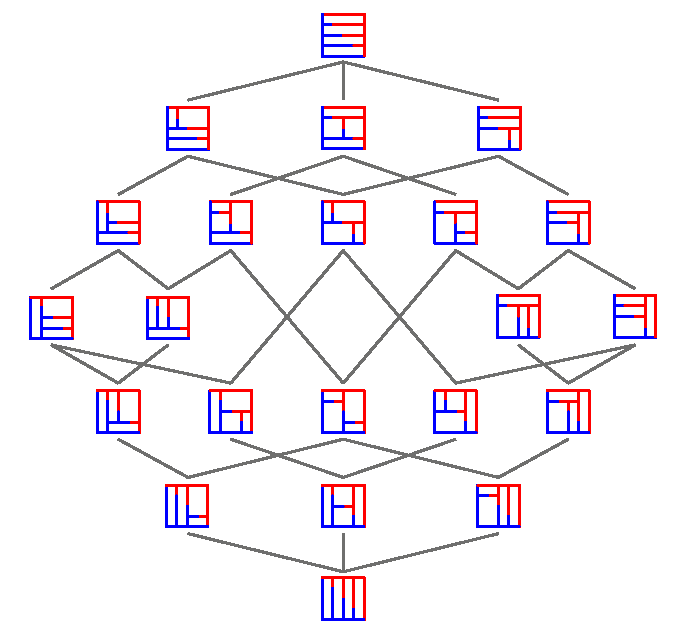
\includegraphics[scale=.9]{weakRectangulationLattice}}
	\caption{The weak rectangulation lattice.}
	\label{fig:weakRectangulationLattice}
\end{figure}

\begin{figure}
	\centerline{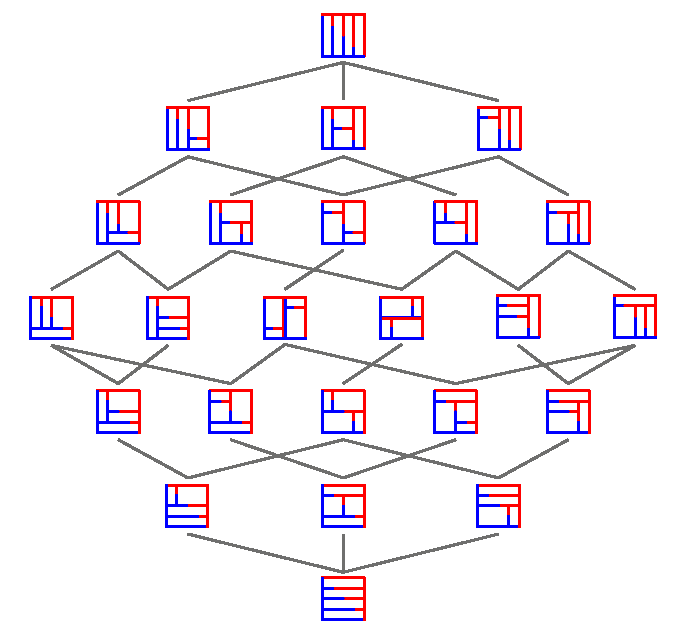
\includegraphics[scale=.9]{strongRectangulationLattice}}
	\caption{The strong rectangulation lattice.}
	\label{fig:strongRectangulationLattice}
\end{figure}

\end{document}
